\documentclass[14pt]{extreport}
\usepackage{xcolor}
\usepackage{float}
\usepackage{graphicx}
\usepackage{caption}
\usepackage{subcaption}
\linespread{1}
\usepackage[utf8]{inputenc} 
\usepackage[T1]{fontenc}
\usepackage{amsmath}
\usepackage{mathtools}
\usepackage{hyperref}
\usepackage{listings}
\begin{document}

% Name of your university/college
\begin{center}
	
\textsc{\Large \textbf{Machine Learning\\}}

\textsc{\Large \textbf{Academic Year 2019-2020 \\}}

\textsc{\Large \textbf{Technical University of Munich \\}}

\textsc{\Large \textbf{\it{Luca Corbucci\\}}}
\end{center}
 
\tableofcontents

\chapter{Lezione 1 - Knn}

Parlando di modelli di Machine learning possiamo fare una prima distinzione tra:
\begin{itemize}
\item Parametric model: in un parametric model fissiamo già fin dall’inizio il numero di parametri da utilizzare e questi parametri non variano quando
crescono i dati che abbiamo a disposizione. Un modello di questo genere fa assunzioni molto forti ma è rapido da utilizzare.
\item Non-parametric model: in un non-parametric model invece abbiamo che la quantità di parametri cresce in base alla quantità di dati che abbiamo a
disposizione. Un modello di questo genere è più flessibile ma possono essere complicati dal punto di vista computazionale.
\end{itemize}

Un modello non parametrico molto famoso è il K-nn. 
Quando dobbiamo creare un certo modello di machine learning la prima cosa che dobbiamo fare è
partire dai dati cercando di studiare la distribuzione dei dati che abbiamo a disposizione. È importante anche capire in che modo le feature che
vogliamo considerare mi possono differenziare i vari dati. Ad esempio possiamo avere uno scatter plot come questo:

\begin{figure}[H]
\centering
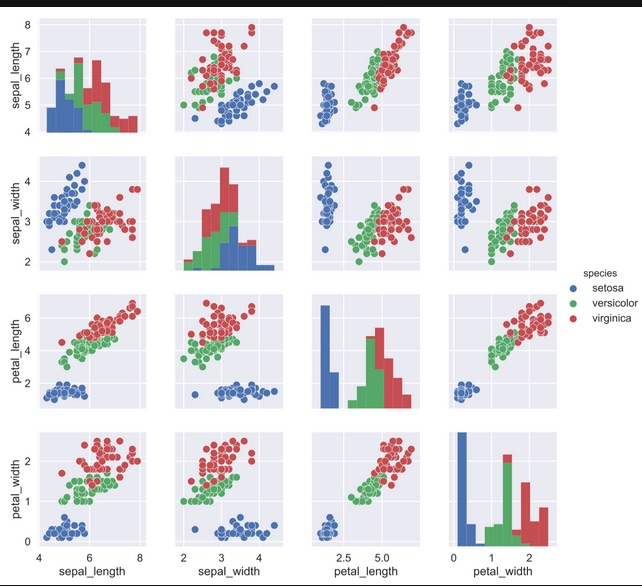
\includegraphics[width=0.7\linewidth]{55.jpeg}
\end{figure}

In cui sulla diagonale abbiamo i grafici che mi mostrano la frequenza del tipo di dato in base alle varie feature che consideriamo. Possiamo anche
creare dei grafici in cui confrontiamo due feature per capire in che modo i nostri dati sono distribuiti all’interno del grafo. Ad esempio potremmo
avere vari cluster di dati differenti tra loro e questi possono essere utili se vogliamo classificare una nuova istanza che non abbiamo ancora visto.


\begin{figure}[H]
\centering
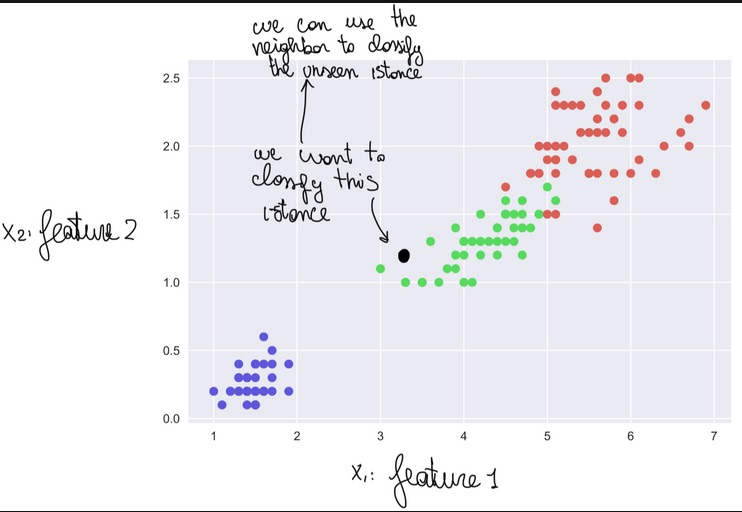
\includegraphics[width=0.7\linewidth]{56.jpeg}
\end{figure}

Una possibile soluzione per classificare una istanza che non abbiamo ancora mai visto è considerare la distanza di questa istanza dai punti che gli
sono vicini e poi andare a scegliere la classificazione migliore in base a quanti punti sono di un certo tipo o di un altro, questo algoritmo di
classificazione è chiamato K-nn.

\section{K-nn}

K-nn è un algoritmo di supervised machine learning perchè i dati che abbiamo per fare il training del modello sono già classificati. In questo
algoritmo abbiamo dei dati di training $D = {(x_i, y_i)}^N_{i=1}$ dove xi è l’insieme delle feature che stiamo considerando e yi è la classificazione
che abbiamo per quella specifica istanza. 
Per classificare una nuova osservazione svolgiamo i seguenti passaggi: 
\begin{itemize}
	\item Definiamo una misura per il calcolo della distanza, una possibile è la distanza Euclidea; 
	\item Prendiamo l’instanza da classificare e calcoliamo la distanza di questa istanza da tutti gli altri dati di training [NON SOLO K PUNTI, DEVO CALCOLARE LA DISTANZA DA TUTTI I PUNTI]; 	
	\item Poi una volta calcolata la distanza da tutti i punti prendo i K che sono più vicini a me e classifico la nuova istanza in base ai miei K vicini.
\end{itemize} 

K-nn è un algoritmo che funziona sia nel caso di classificazione sia nel caso di regressione.

\begin{figure}[H]
\centering
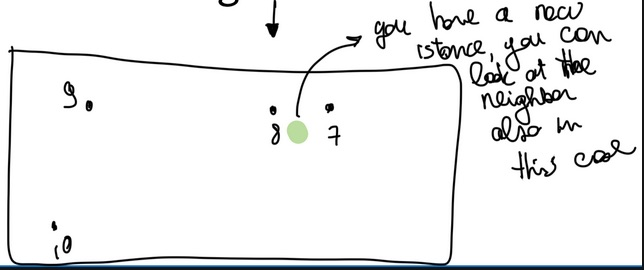
\includegraphics[width=0.7\linewidth]{57.jpeg}
\end{figure}

In particolare nel caso della regressione possiamo comunque rappresentare i miei dati nel piano e posso comunque rappresentare anche la nuova istanza
e prendere la distanza dagli altri punti classificando l’istanza in base ai K punti più vicini.

La K che scegliamo per l’algoritmo K-nn può essere un qualsiasi numero, ad esempio potremmo prendere K = 1, in questo caso per classificare una nuova
istanza consideriamo solamente l’istanza già classificata più vicina. Quello che posso produrre in questo caso è una decision region che corrisponde
alla Voronoi tassellation, per ognuna delle parti in cui divido il piano ho solamente un punto, le regioni sono divise da un decision boundary che
quindi separa le classi.

\begin{figure}[H]
\centering
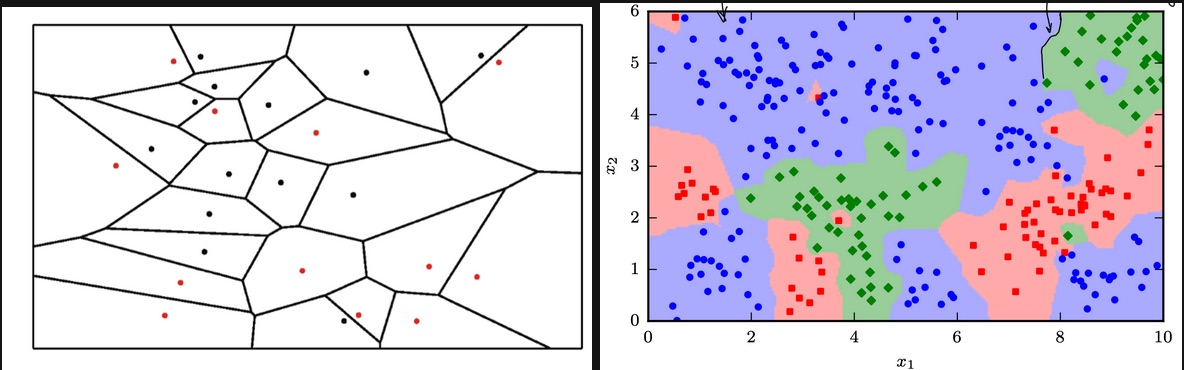
\includegraphics[width=0.7\linewidth]{58.jpeg}
\end{figure}

Utilizzare K=1 è chiaramente un problema perchè otteniamo un modello che non generalizza e in particolare avremo problemi con il rumore perchè ad
esempio nella figura di destra abbiamo un solo punto rosso in mezzo a tanti punti blu, se mi capita una istanza da classificare che finisce nella zona
del punto rosso, questa verrà classificata come rossa anche se quel punto è chiaramente rumore. Dato che il nostro obiettivo è generalizzare non
possiamo utilizzare K = 1.

\section{Formula per il K-nn}

Quindi, in generale la formula per il K-nn è la seguente:

\begin{figure}[H]
\centering
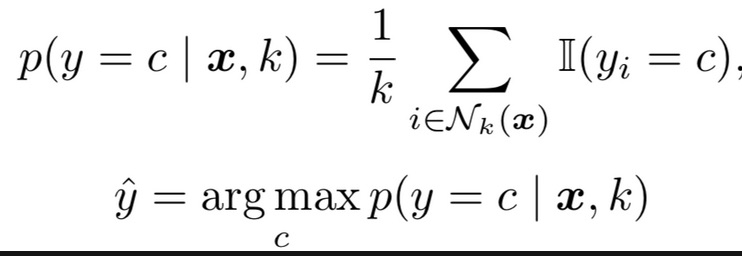
\includegraphics[width=0.7\linewidth]{59.jpeg}
\end{figure}

Dobbiamo calcolare la probabilità che una nuova istanza x appartenga ad una classe c dato x e il parametro K. Consideriamo i K vicini di x $N_k(x)$
e per ognuno di essi contiamo quanti appartengono alla classe c. 
$$I(y_i = C)$$ 
vale 1 se yi = c altrimenti vale 0.

Una volta ottenuta la somma dividiamo per k perchè vogliamo normalizzare per ottenere una distribuzione della probabilità. In questo modo dividendo per k, la somma delle varie probabilità sarà sempre 1.
Una volta calcolate tutte le probabilità cerchiamo quella che ha probabilità maggiore e quella mi indicherà l’appartenenza della nuova istanza alla classe c.
In pratica per classificare, se non ci serve esplicitamente la probabilità, possiamo evitare di dividere per k e prendere semplicemente la classe che compare di più nei K vicini dell’istanza che dobbiamo classificare, ovvero assegnamo alla nuova istanza la moda dei label dei vicini.

\subsubsection{Cost sensitive Learning}
Possiamo trovarci in una situazione in cui abbiamo due possibili classi che però sono sbilanciate, nel senso che l’$80\%$ dei dati appartengono alla classe BLU e il $20\%$ alla classe VERDE.
In questo caso possiamo calcolare di quanto sono sbilanciati i due set di dati, ad esempio in questo caso un set è 4 volte l’altro e poi quando dobbiamo classificare usiamo il cost sensitive learning nel senso che se ho K = 10 e ho che 6 vicini sono BLU e 4 sono VERDI, moltiplico il numero dei verdi per 4 e alla fine classifico il punto come VERDE.
\subsubsection{Weighted K-nn} 
Quando usiamo K-nn potremmo renderci conto che stiamo considerando K vicini di cui, alcuni poco distanti da noi, altri molto distanti da noi.
In generale possiamo dire che i vicini meno distanti da noi dovrebbero avere un peso più grande nel momento in cui classifichiamo la nuova istanza, quindi nella formula precedente possiamo aggiungere una nuova componente che faccia in modo che non conti solamente il numero dei vicini classificati in una certa classe ma anche la distanza di quei vicini dalla nuova istanza da classificare.
La formula quindi diventa


\begin{figure}[H] 
	\centering
	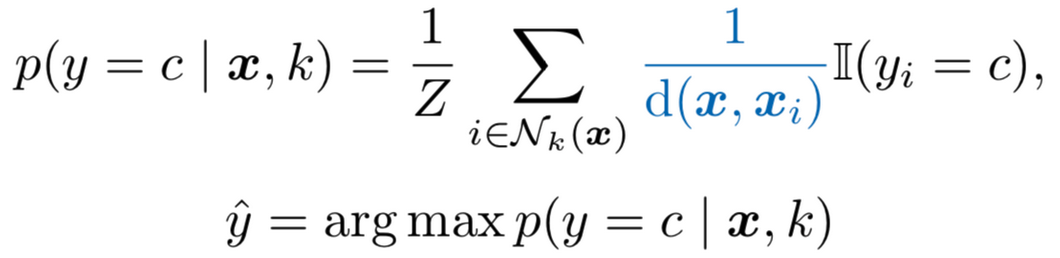
\includegraphics[width=0.7\linewidth]{451.jpeg}
	\end{figure}

	La I(y = c) viene moltiplicata per l’inverso della distanza tra l’istanza x da classificare e l’istanza xi che è uno dei nostri K vicini che consideriamo.
	In questo modo se la distanza tra i due punti è piccola avremo un peso molto grande da moltiplicare per I(y=c), se invece la distanza è grande abbiamo un peso piccolo.
	Quindi questo fattore che usiamo per moltiplicare è inversamente proporzionale alla distanza.
	Tutta la sommatoria poi va moltiplicata per 1/Z dove in questo caso Z è la sommatoria dell’inverso della distanza tra l’instanza da classificare e le altre nel vicinato:


\begin{figure}[H] 
	\centering
	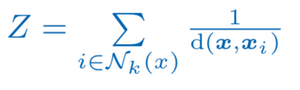
\includegraphics[width=0.7\linewidth]{452.jpeg}
	\end{figure}

	Anche in questo caso questa moltiplicazione ci serve per ottenere una probabilità, la somma di tutte le probabilità per le varie classi sarà 1.

\subsubsection{K-nn per regressione}

Come visto si può usare K-nn anche per la regressione

In questo caso la formula per il K-nn diventa la seguente:


\begin{figure}[H] 
	\centering
	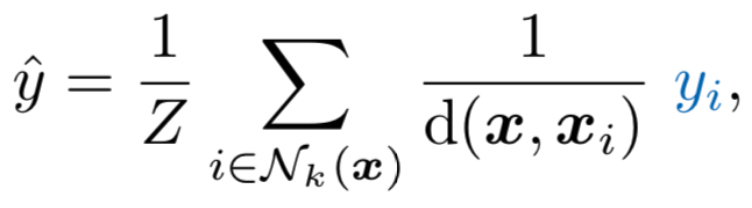
\includegraphics[width=0.7\linewidth]{453.jpeg}
	\end{figure}

	Al posto della I(yi=c) abbiamo semplicemente yi dove con yi intendiamo il valore che è assunto dai vari punti che sono nel vicinato dell’istanza che vogliamo classificare.
	Anche in questo caso stiamo considerando il caso pesato e quindi moltiplichiamo ogni volta per l’inverso della distanza e alla fine, ottenuta la somma completa, dividiamo per la somma di tutte le distanze (della nuova istanza dai K vicini).
	Quindi alla fine abbiamo che la nuova istanza verrà classificata come la media dei valori dei K vicini moltiplicata per l’inverso della distanza dell’istanza dai vicini. 

\subsubsection{Come scegliere la K migliore?} 

Dato che il nostro obiettivo è generalizzare, dobbiamo cercare la K che ci permette di avere una migliore generalizzazione sui dati che non ho ancora visto.
La K in questo caso è chiamata Iper-parametro.
Dato che non abbiamo a disposizione i dati futuri che vorrò usare con il mio modello, posso dividere i dati che ho in due parti principali:

\begin{itemize}
	\item Learning Set, a sua volta diviso in:
		\begin{itemize}
		\item Training Set: generalmente rappresenta l’$80\%$ dei dati, abbiamo differenti iper parametri K e creiamo vari modelli che si differenziano tra loro per la K. Quindi facciamo il training del modello con varie K.
		\item Validation Set: In genere è il $10\%$ dei dati. Ora che abbiamo vari modelli, li testiamo con i dati che sono presenti all’interno del validation set e scegliamo il miglior modello (in base a metriche come l’accuracy) ovvero quello con la K che generalizza meglio.
		Come scelgo la K?
		
\begin{figure}[H] 
	\centering
	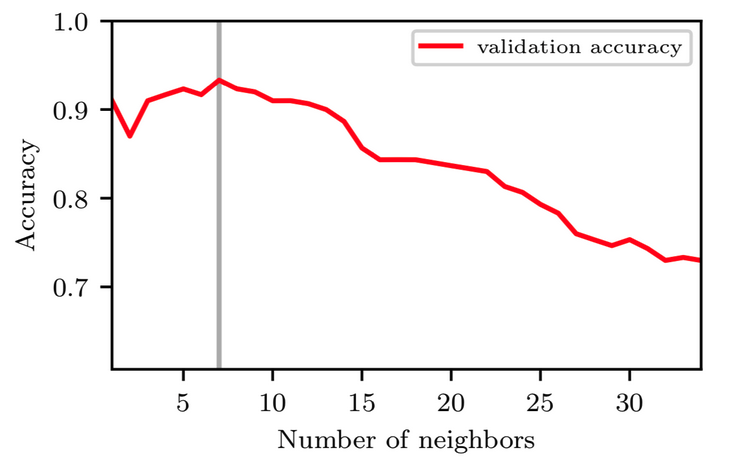
\includegraphics[width=0.7\linewidth]{454.jpeg}
	\end{figure}
	Nel momento in cui ho provato i vari modelli con i dati del validation set posso fare un grafico in cui mostro come varia l’accuracy in base alla variazione della K e poi scelgo la K che ha la migliore accuracy.

		\end{itemize}
	\item Test Set: questo in genere è il $10\%$ dei dati. Ora che abbiamo scelto quello che per noi è il modello migliore possiamo prendere il test set e vedere come generalizza il nostro modello con il test set. 
	Questo è un test finale che faccio per capire come si comporta il modello con dati nuovi, È FONDAMENTALE CHE I TEST CHE FACCIO CON IL MIO MODELLO USANDO IL TEST SET NON VADANO A MODIFICARE GLI IPER PARAMETRI. In pratica non possiamo utilizzare il test set durante la learning phase e non posso scegliere i parametri in base ai dati di test perchè sarebbe come barare.
	Se le performance sul test set non sono buone ci sono varie situazioni possibili:
	\begin{itemize}
		\item Se le performance sul test set non sono buone, in teoria dovrei osservare performance non buone anche sul validation set perchè la distribuzione dei dati nei due set è simile.
		\item Se invece non sono buone solamente nel test set vuol dire che magari la distribuzione dei dati è molto diversa tra test set e validation set e per questo problema al momento non c’è soluzione.
		\item È poco comune ottenere un risultato non buono a causa dell’overfitting su validation set e su training set perchè è poco comune che allo stesso tempo si ottenga overfitting sia sul training set che sul validation set, di solito si ottiene solamente su uno dei due set ma poi non arrivo al test sul test set perchè devo cambio i parametri per evitare l’overfitting.
		\end{itemize} 
	\end{itemize}


	\begin{figure}[H] 
		\centering
		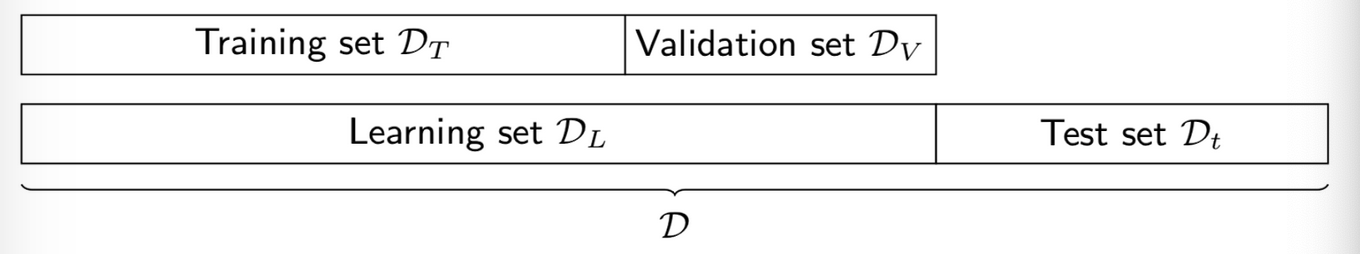
\includegraphics[width=0.7\linewidth]{455.jpeg}
		\end{figure}

Come si fa a dividere i dati:
\begin{itemize}
	\item Random Sampling: divisione random in set di dati, il problema in questo caso è che potrei fare un set di dati dove ci sono solamente dati di una certa classe.
	\item Stratified Sampling: divisione che cerca di preservare la distribuzione delle classi all’interno dei set di dati che vengono creati.
		Se facciamo la test validation è molto meglio usare lo stratified sampling.
	\end{itemize}
		
	\subsubsection{Misure di performance}

	Per capire le performance di un algoritmo di classificazione (binario) possiamo creare la confusion table (confusion matrix) ovvero una tabella in cui illustriamo le differenti combinazioni di risultati che possiamo ottenere.
	Nella tabella abbiamo che i risultati TP (True positive) e TN (True negative) sono quelli positivi perchè sono delle istanze che sono state correttamente riconosciute come positive e come negative.
	Al contrario invece i casi False negative e False positive sono negativi perchè sono quelle istanze che sono state riconosciute come negative ma in realtà sono positive e quelle riconosciute come positive quando in realtà sono negative. 
	


	\begin{figure}[H] 
		\centering
		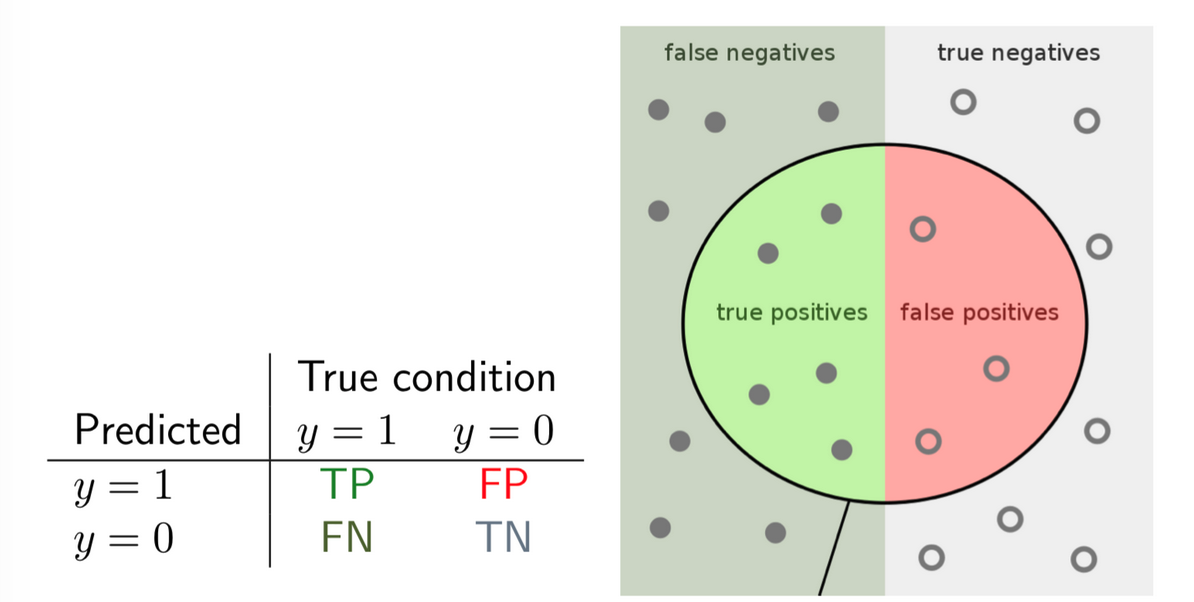
\includegraphics[width=0.7\linewidth]{456.jpeg}
		\end{figure}

Partendo dalla confusion table poi possiamo definire varie possibili metriche che possono essere utilizzate per comprendere le performance di un certo modello:

\begin{itemize}
	\item L’accuracy è definita in questo modo: 
	\begin{figure}[H] 
	\centering
	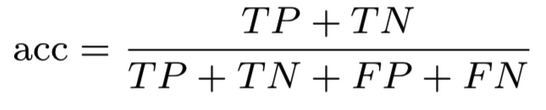
\includegraphics[width=0.7\linewidth]{457.jpeg}
	\end{figure}
	In questo caso noi stiamo considerando le istanze che sono state classificate correttamente (TP+TN) rispetto a tutte le istanze che sono state classificate.
	Per andare bene dovremmo avere una accuracy alta ed è compresa tra 0 e 1.
	\item Precision: è calcolata come:
	\begin{figure}[H] 
	\centering
	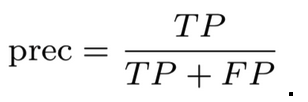
\includegraphics[width=0.7\linewidth]{458.jpeg}
	\end{figure} 
	La precision mi indica quanti sono i risultati rilevanti per il mio modello.
	Questo vuol dire che noi stiamo prendendo in considerazione i casi che sono stati classificati come positivi e che lo sono realmente (TP) rispetto a quelli che sono stati classificati positivi dal mio algoritmo (considerando quindi anche i falsi positivi). Nel caso di una classificazione di una malattia, consideriamo quelli che ho classificato malati e lo sono realmente diviso quelli che ho classificato malati e lo sono realmente più quelli classificati malati che però stanno bene.
	Se io qua classifico tutti come positivi ho una precision che è pessima perchè avrò un’alta percentuale di falsi positivi.
	\item Recall: è definita in questo modo:
	\begin{figure}[H] 
	\centering
	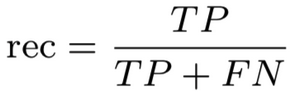
\includegraphics[width=0.7\linewidth]{459.jpeg}
	\end{figure}
	Qua la recall mi indica quanti sono i risultati che sono rilevanti e che sono stati classificati correttamente.
	Qua stiamo considerando i true positivi rispetto a quelli che dovrebbero essere classificati come positivi. Quindi, se il mio modello sbaglia a classificare e mi segna come negativi tanti che in realtà sarebbero positivi la recall si abbassa. Se segno tutti come negativi ad esempio avrò una recall pessima perchè FN sale molto.
\end{itemize}


In generale si può dire che quando la recall sale, la precision scende, l’esempio più classico è classificare tutti come positivi, in questo modo la recall sarà massima perchè abbiamo che i Falsi negativi sono 0. Allo stesso tempo però la precision sarà minima perchè abbiamo tantissimi falsi positivi.
Quindi l’idea è che dobbiamo scegliere un modello che considera un trade off tra precision e recall e per fare questa scelta possiamo utilizzare ad esempio un grafico in cui mettiamo sulla X la precisione e sulla Y la recall. Creando un grafico per ogni differente approccio per la classificazione possiamo fare un confronto tra i vari algoritmi e scegliere il migliore.

Consideriamo la curva che si forma al variare di K (nel caso di K-nn) e preferiamo il modello che ha l’area più grande sotto la curva.
Il caso ottimo è quello in cui  abbiamo sia la precision sia la recall fissate a 1, perchè l’area sotto la curva è massima.


\begin{figure}[H] 
	\centering
	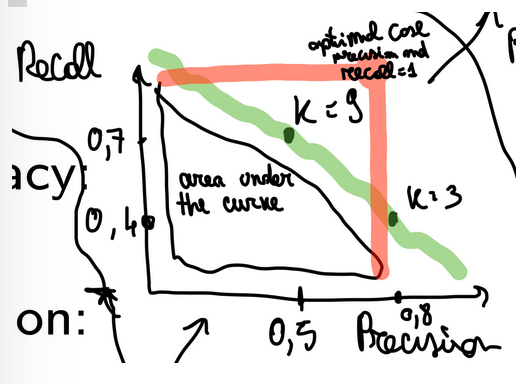
\includegraphics[width=0.7\linewidth]{460.jpeg}
	\end{figure}

	Se vogliamo una metrica che mi considera allo stesso tempo sia la precision sia la recall cercando di massimizzarle allora devo utilizzare l’F1 Score (che in pratica fa la media armonica). L’F1 Score è definito come:


\begin{figure}[H] 
	\centering
	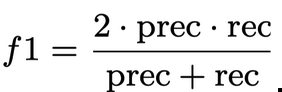
\includegraphics[width=0.7\linewidth]{461.jpeg}
	\end{figure}

	Altre possibili metriche sono le seguenti:
	

	\begin{figure}[H] 
		\centering
		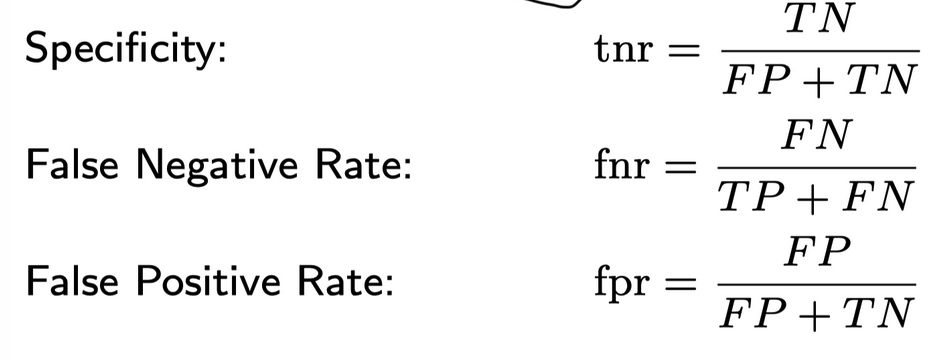
\includegraphics[width=0.7\linewidth]{462.jpeg}
		\end{figure}

		C’è da fare poi una considerazione importante su queste metriche perchè non sempre possiamo prendere il risultato che ci offrono senza ragionarci.
In particolare quando abbiamo una situazione con quantità di dati molto sbilanciate, ad esempio il $90\%$ dei dati sono BLU e il $10\%$ VERDI, ci troviamo con un classificatore che potrebbe classificare tutto come BLU e otterremmo comunque una classificazione corretta nel $90\%$ dei casi.
Quindi è importante che prima di iniziare a fare classificazioni si studino i dati che si hanno a disposizione in modo da capire se sono bilanciati o meno.

	
	\subsubsection{Distance Measure} 

	Per calcolare la distanza tra le istanze quando usiamo K-nn ci sono varie possibili metriche:

	\begin{itemize}
		\item Distanza euclidea: è definita in questo modo:
		
\begin{figure}[H] 
	\centering
	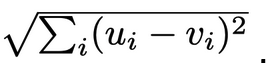
\includegraphics[width=0.7\linewidth]{463.jpeg}
	\end{figure}
		Con la distanza Euclidea quello che si fa è posizionarsi sul punto che vogliamo classificare e poi considerare l’ipersfera centrata in quel punto. Poi aumentiamo il raggio dell’ipersfera fino a quando non contiene tutti i K punti che vogliamo considerare.
	
\begin{figure}[H] 
	\centering
	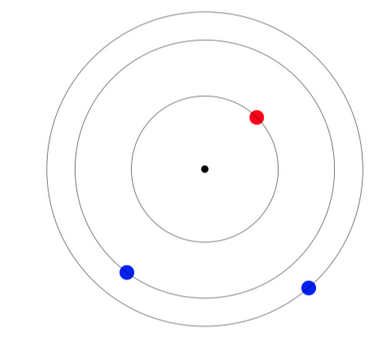
\includegraphics[width=0.7\linewidth]{466.jpeg}
	\end{figure}
		\item 	Possiamo usare la norma 1
	\item Possiamo usare la norma infinita
	\item Possiamo usare anche l’angolo
	
\begin{figure}[H] 
	\centering
	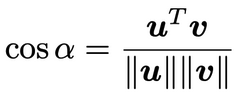
\includegraphics[width=0.7\linewidth]{465.jpeg}
	\end{figure}
	\item Ci sono poi edit distance e Hamming Distance
	\item Poi c’è la Mahalanobis distance definita così:
	
\begin{figure}[H] 
	\centering
	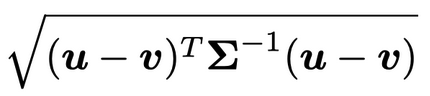
\includegraphics[width=0.7\linewidth]{464.jpeg}
	\end{figure}
	Questa misura della distanza prende in considerazione anche la matrice di covarianza (la parte dopo la sommatoria) e quindi in pratica considera anche se gli attributi delle istanze sono correlati tra loro o no.
	Se sono correlati grazie alla parte dopo la matrice di covarianza, possiamo eliminare gli attributi ridondanti.
	Rispetto alla distanza Euclidea, questa di Mahalanobis va a creare una sorta di ellisse attorno al punto che vogliamo classificare.
	Rispetto alla distanza Euclidea vengono scalati gli assi e quindi questo ci permette di evitare il problema che abbiamo con la distanza Euclidea che non scala gli assi e quindi non considera mai il modo in cui i dati sono distribuiti.
	
	\end{itemize} 

	
	\begin{figure}[H] 
	\centering
	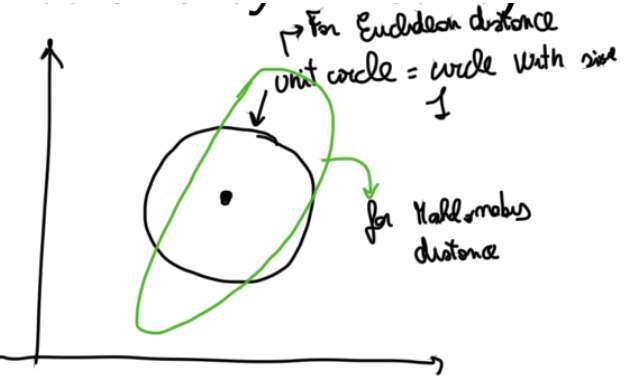
\includegraphics[width=0.7\linewidth]{467.jpeg}
	\end{figure}
	In generale dove possiamo usare uno di questi algoritmi per il calcolo della distanza, possiamo anche usare la classificazione per gestire istanze sconosciute.

	\subsubsection{Interpretazione probabilistica di K-nn}

	Possiamo pensare al K-nn anche in termini di probabilità, consideriamo il caso di avere due classi possibili e calcoliamo per prima cosa la probabilità di avere una certa istanza o l’altra (si chiama mixture model ovvero calcoliamo la probabilità di avere una certa sub popolazione all’interno della mia popolazione complessiva):

	\begin{figure}[H] 
		\centering
		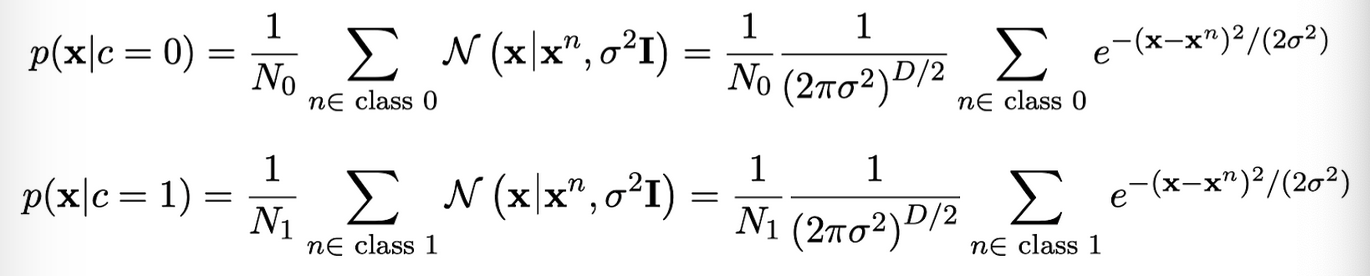
\includegraphics[width=0.7\linewidth]{468.jpeg}
		\end{figure}

		In questi due calcoli stiamo considerando una distribuzione normale dei dati e per ottenere la probabilità normalizziamo dividendo per il numero di istanze che abbiamo appartenenti a quella classe.
		Nei due calcoli consideriamo una varianza $\sigma^2$ quindi per ogni istanza di training calcoliamo il numero di istanze 0 e 1 
		all’interno della "isotropic gaussian" con larghezza $\sigma^2$ e questo mi permette di indicare la probabilità che quell’istanza di trainining sia classificata come 0 o come 1.
		
		Questa stima della probabilità è chiamata “Parzen Estimator” e modella la distribuzione dei dati come una somma (pesata in modo uniforme) delle distribuzioni centrate nel punto di training x.
		In ogni punto di training mettiamo una gaussiana con varianza $\sigma^2$, la larghezza di questa gaussiana è rappresentata dal cerchio che creo in ognuno dei punti.



\begin{figure}[H] 
\centering
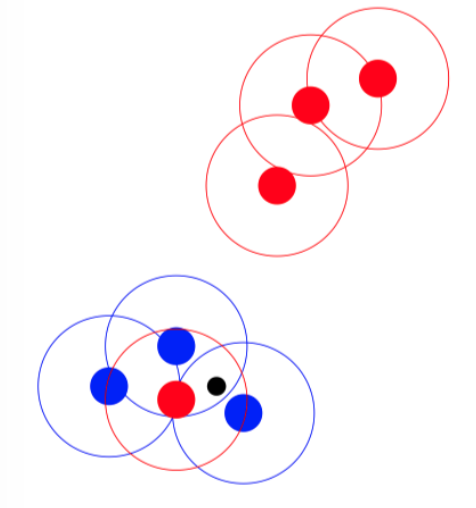
\includegraphics[width=0.7\linewidth]{469.jpeg}
\end{figure}

Quando vogliamo calcolare un nuovo punto x* (nero nella figura) possiamo usare il teorema di Bayes:


\begin{figure}[H] 
	\centering
	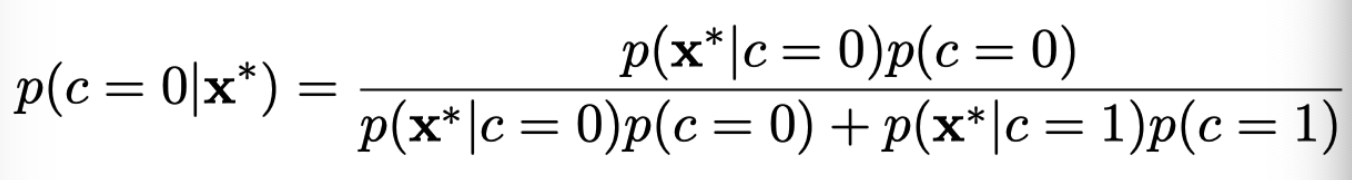
\includegraphics[width=0.7\linewidth]{470.jpeg}
	\end{figure}

	La stessa formula la applichiamo per capire la probabilità di avere l’altra classe.
	Nella formula p(c=0) e p(c=1) viene calcolata come N0/(N0+N1) e N1/(N1+N0).
	Alla fine quello che vogliamo fare è assegnare una classe alla nuova istanza x* quindi quello che si fa è dividere le due probabilità, se il risultato è maggiore di 1 classifichiamo come 0, altrimenti classifichiamo come 1.
	

\begin{figure}[H] 
	\centering
	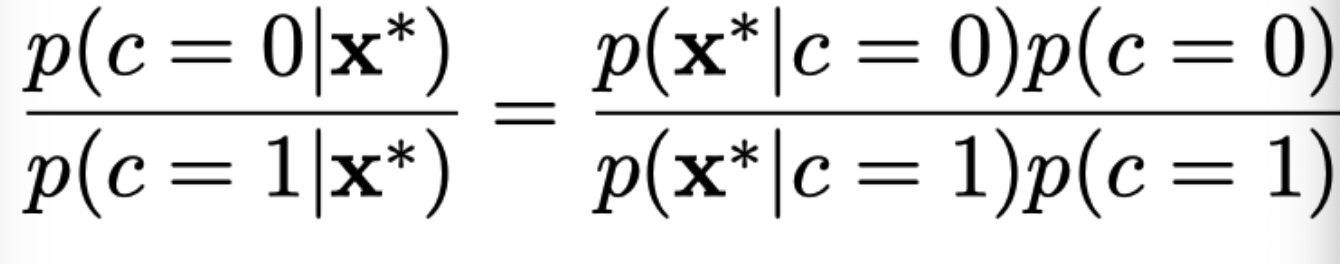
\includegraphics[width=0.7\linewidth]{471.jpeg}
	\end{figure}


	\subsection{Problemi noti}

	\subsubsection{Scaling Issue}
	
	Quando utilizziamo la distanza euclidea e ci troviamo con dei dati che hanno una scala differente per le varie feature che dobbiamo considerare, potremmo trovarci in una situazione simile a quella della foto:

	\begin{figure}[H] 
		\centering
		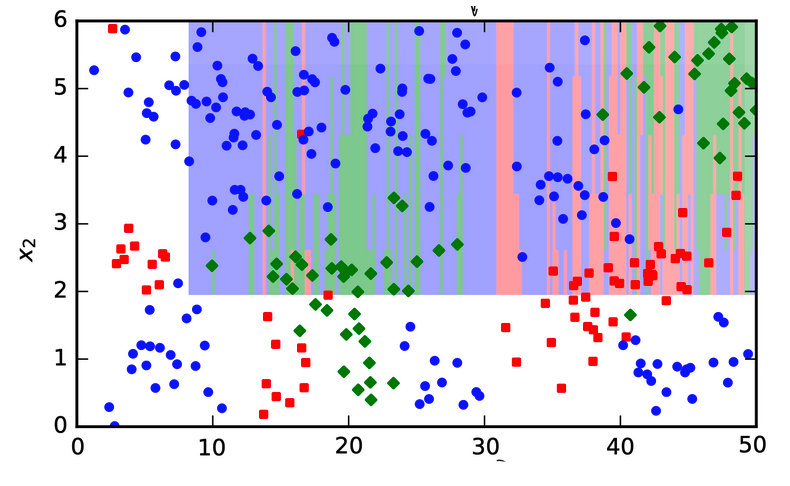
\includegraphics[width=0.7\linewidth]{472.jpeg}
		\end{figure}

		In questo caso infatti stiamo calcolando le distanze tra due feature però la feature X1 ha valori compresi tra 0 e 50 mentre la X2 tra 0 e 6 e quindi otteniamo queste specie di striscie verticali.
		Per risolvere questo problema ci sono due possibili soluzioni:

		\begin{itemize}
			\item Usare la normalizzazione per standardizzare i dati, in questo modo riusciamo a ridurre la scala di tutte le feature che vogliamo considerare a valori compresi tra 0 e 1. Questa procedura è piuttosto standard e ci sono vari metodi per eseguirla, abbiamo la 0,1 normalization o anche lo 0 score normalization.
			
\begin{figure}[H] 
	\centering
	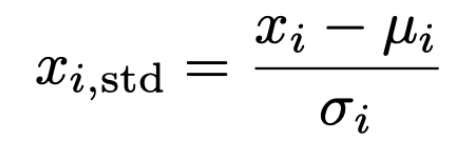
\includegraphics[width=0.7\linewidth]{473.jpeg}
	\end{figure}
			\item Usare la distanza di Mahalanobis, in questo modo otteniamo lo stesso risultato che abbiamo con la normalizzazione perchè la matrice di covarianza è uguale alla distanza euclidea calcolata sui dati normalizzati.

			\end{itemize}

			\subsubsection{Curse of Dimensionality}
			
			Si tratta di un problema di spazio vuoto, abbiamo un dominio discreto, ad esempio immagini nello spazio, se il numero di queste immagini è finito e vogliamo rappresentarle in una sola dimensione, avremo che queste immagini copriranno totalmente lo spazio.
			Se passo ad una rappresentazione in due dimensioni avrò dello spazio vuoto, questo aumenta ancora di più se aggiungo un’altra dimensione ancora.
			Quando aggiungo nuove dimensioni lo spazio vuoto cresce in modo esponenziale, la stessa cosa non si può dire dei dati che non crescono in modo esponenziale da poter coprire tutto lo spazio vuoto.
			
			Questo può essere un problema per K-nn perchè se siamo con 3 dimensioni e abbiamo la nostra istanza in un certo punto isolato del piano, finiremo per classificarla basandoci su istanze che sono in realtà molto lontane da questa istanza e quindi faremmo probabilmente un errore.

			
\begin{figure}[H] 
	\centering
	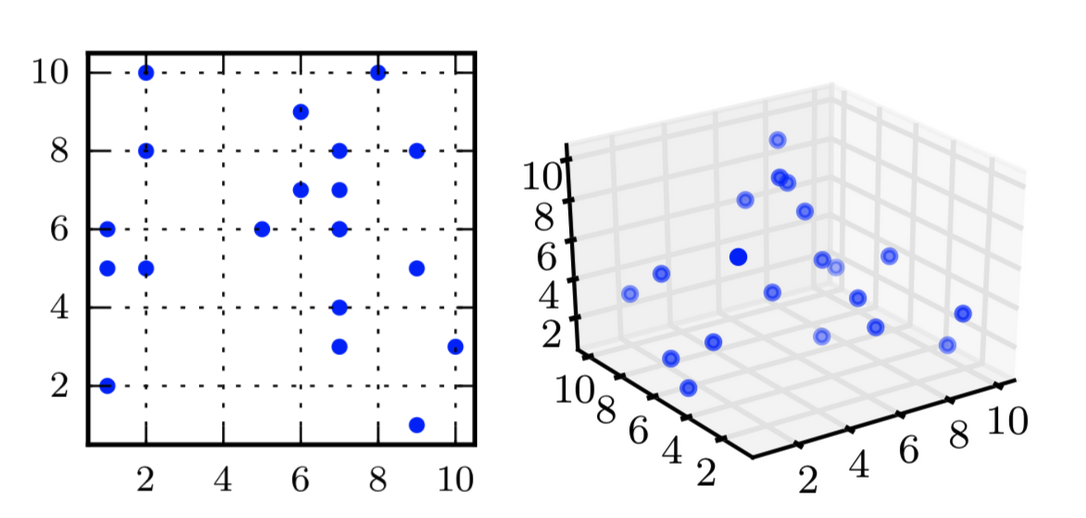
\includegraphics[width=0.7\linewidth]{474.jpeg}
	\end{figure}

	\subsection{Considerazioni su K-nn}

	Concludendo possiamo fare alcune considerazioni sull’uso di K-nn:
	\begin{itemize}
		\item L’algoritmo mi costringe a portarmi dietro tutto il dataset di training per fare le successive classificazioni, quindi ho un costo in termini di memoria di O(N).dove N è il numero di punti nel piano.
		Ci sono delle possibili ottimizzazioni, ad esempio c’è un metodo chiamato data editing che mi permette di rimuovere i punti che non sono interessanti o utili per la classificazione.
\item Ci sono dei metodi per comprimere i dati che devo memorizzare senza portarmi dietro tutti i dati di training.
\item Ci sono delle possibili ottimizzazioni che mi fanno usare una struttura di ricerca ad albero per approssimare in modo efficiente il funzionamento di K-nn.
		\end{itemize}Per ogni punto che voglio classificare devo calcolare la distanza da tutti i punti che stanno nel piano, quindi è un costo O(N) dove N è il numero di punti nel piano.


\chapter{Decision Tree}

\section{Introduzione}

I decision trees rappresentano un altro possibile modello da poter utilizzare per la classificazione o la regressione.
I decision tree sono utilizzati per svariati motivi:

\begin{itemize}
	\item Possono modellare le relazioni tra i dati senza fare assunzioni a priori
	\item Possono gestire dati eterogenei
	\item Implementano in modo automatico la feature selection
	\item Sono robusti quando nei dati ci sono errori e outlier
\end{itemize} 


In questo caso l’idea è quella di andare a partizionare ricorsivamente lo spazio degli input per definire un modello in ognuna delle regioni risultati.
Questo partizionamento dello spazio può essere rappresentato facilmente con un albero.
Questo modello può essere definito con la seguente equazione:


\begin{figure}[H] 
	\centering
	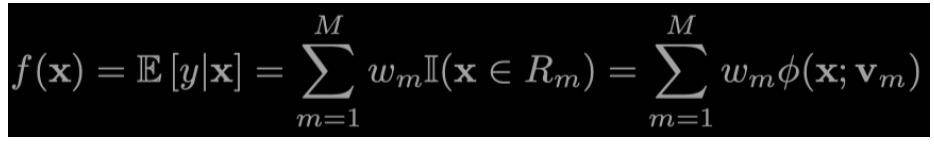
\includegraphics[width=0.7\linewidth]{475.jpeg}
	\end{figure}

	Dove:
	\begin{itemize}
		\item Vogliamo classificare l’istanza x
		\item m è la regione che stiamo prendendo in considerazione
		\item $w_m$ è la risposta media che abbiamo ottenuto in quella regione 
		\item I(x in Rm) è una funzione booleana che mi dice se x è in quella regione o no.
	\end{itemize}


Quindi si tratta di un modello con una funzione che mi definisce le regioni e dei pesi che mi specificano il response value in ognuna delle regioni.
Una rappresentazione alternativa a quella appena vista (che non prevede l’uso dei response value) è quella in cui nelle foglie del nostro albero andiamo a memorizzare la distribuzione dei label dei vari elementi presenti all’interno della regione che stiamo considerando. Ad esempio se ci sono 4 blu e 2 rossi scriveremo (4,2), un esempio:


\begin{figure}[H] 
	\centering
	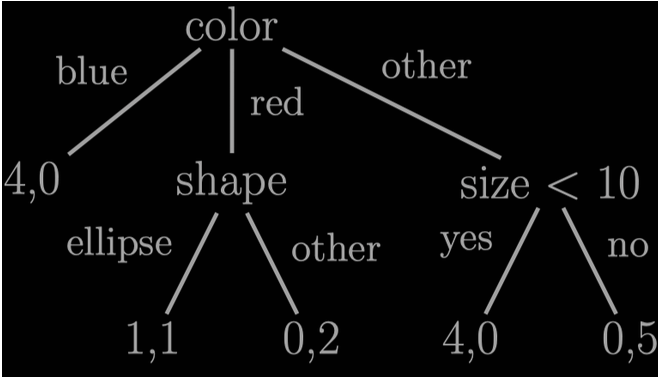
\includegraphics[width=0.7\linewidth]{476.jpeg}
	\end{figure}


	Più in generale possiamo definire un decision tree come un albero in cui abbiamo dei nodi interni che rappresentano le possibili “domande” che possiamo farci basandoci sulle feature che abbiamo a disposizione e poi avremo dei nodi foglia che sono le possibili classificazioni che otteniamo rispondendo ad alcune delle domande.
	Gli archi che collegano i vari nodi sono le possibili risposte alle domande che ci stiamo facendo, ad esempio qua ci chiediamo il tipo di umidità, le possibili risposte sono normale o alta e poi abbiamo due possibili classificazioni che sono “Yes” e “No”.
	Nel secondo esempio abbiamo una classificazione con feature numeriche e in questo caso in base alla risposta che diamo finiamo in una foglia in cui abbiamo prevalenza di classificazioni rosse o in una in cui abbiamo prevalenza verde. 
	Quindi se andiamo a sinistra classifichiamo come rosso e se andiamo a destra come verde.


\begin{figure}[H] 
	\centering
	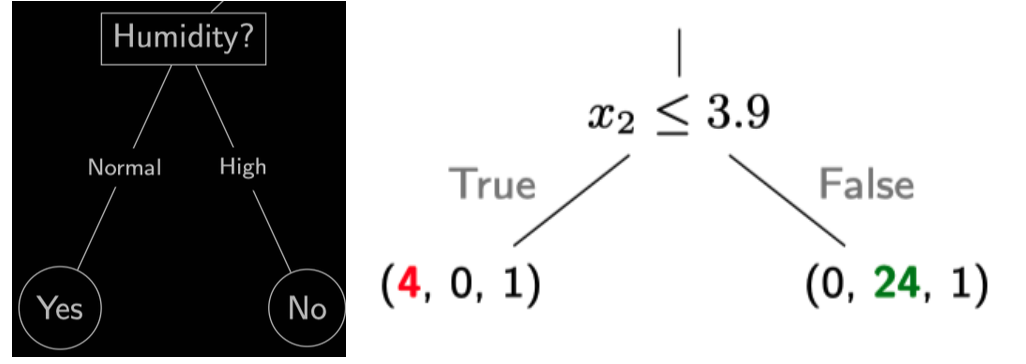
\includegraphics[width=0.7\linewidth]{477.jpeg}
	\end{figure}

	Un esempio, in questo caso abbiamo 3 possibili domande in base alle feature che vogliamo considerare e poi abbiamo 4 possibili classificazioni. 
	L’obiettivo quindi, anche in questo caso, è fare una previsione, con la funzione 
	f: X->Y.
	Se consideriamo l’istanza X = [Fur=Yes, Bark = Yes, Fly = No] abbiamo che il decision tree ci fornisce come risposta Y = dog.



	\begin{figure}[H] 
		\centering
		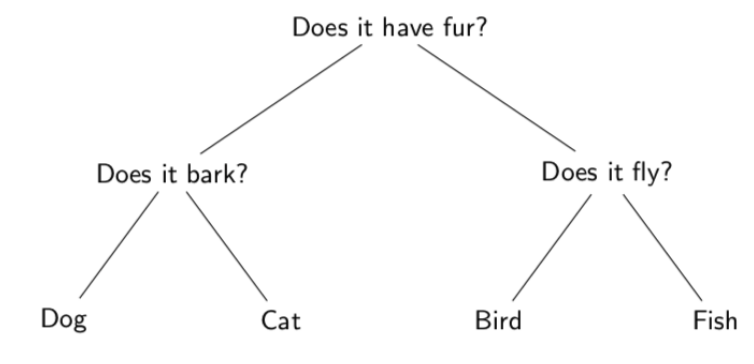
\includegraphics[width=0.7\linewidth]{478.jpeg}
		\end{figure}

		In alcuni casi potrei avere un dataset in cui scegliendo una certa feature ho delle possibili risposte che mi forniscono direttamente l’appartenenza ad una certa classe, in altri casi invece devo fare varie domande prima di arrivare ad una risposta che mi permetta di classificare la nuova istanza.

		I decision tree possono essere utilizzati sia con input categorici che con input numerici:

		\begin{itemize}
			\item Nel caso di input categorici facciamo come con i decision trees dell’esempio precedente e quindi consideriamo una feature e i possibili valori. Possiamo anche andare a splittare in più di 2 differenti risposte, in questo modo però si rischia di ottenere una frammentazione dei dati con il rischio di andare in overfitting.
			\item Nel caso di input numerici invece abbiamo la rappresentazione dei nostri dati all’interno di un piano e possiamo splittare i dati in base a dei range. Per ognuna delle feature ordiniamo i possibili valori in ordine crescente e cerchiamo di suddividere il piano in base ai possibili valori della feature in questione.
			\end{itemize}


			\begin{figure}[H] 
				\centering
				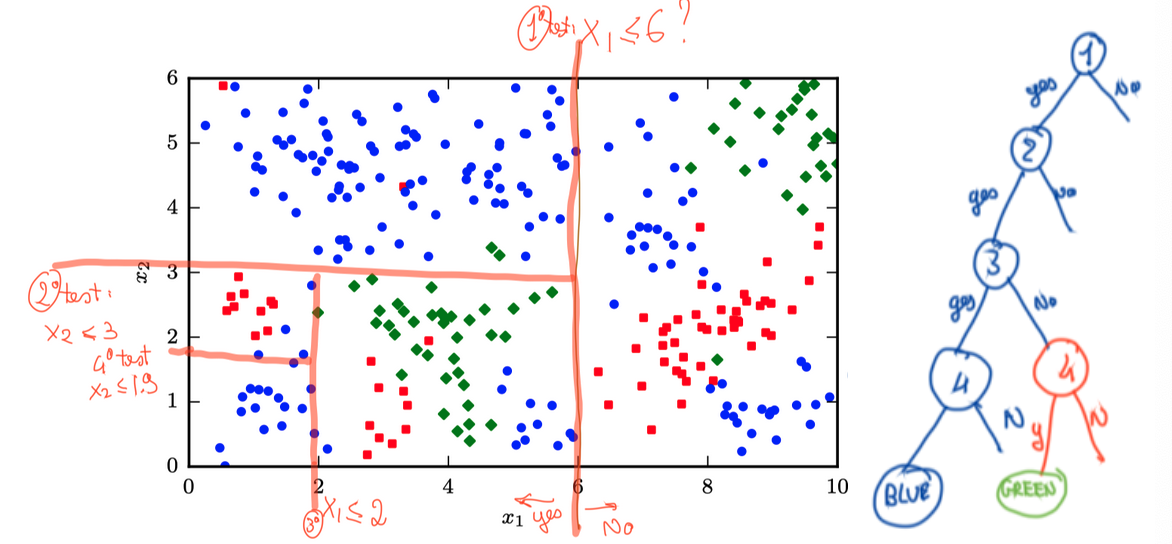
\includegraphics[width=0.7\linewidth]{479.jpeg}
				\end{figure}

				Un esempio con i dati numerici, qua facciamo 4 differenti split ottenendo 5 regioni diverse, nel momento in cui creiamo l’albero cerchiamo di capire in quale regione finiamo e poi in base alla regione in cui siamo finiti classifichiamo l’instanza. 
				Qua, a differenza di quello che succede con il K-nn abbiamo dei decision boundary che sono ben definiti e non abbiamo forme arbitrarie.
				Ad esempio se finiamo nella regione in basso a sinistra possiamo subito classificare come blu, se finiamo in quella nel mezzo tra $xi \leq 6$ e $x1>2$ allora assegnamo verde perchè è la classificazione che compare maggiormente.
				In tutti questi casi per splittare stiamo considerando una funzione che è molto semplice e che quindi prevede solamente una feature alla volta.
				In principio potremmo anche utilizzare funzioni più complicate, ad esempio $x_1+x_2 < 3$ oppure anche $x_2 +\sqrt{x} \leq 4$, in pratica però non vogliamo utilizzare questo tipo di funzioni perchè diventerebbe complicato e costoso calcolare il l’albero di decisione e avremmo una esplosione dei possibili cammini all’interno dell’albero.
				
				\section{Inferenza con i decision tree}

				L’obiettivo della creazione di un decision tree è la classificazione di nuove istanze, quindi la generalizzazione.
Il processo che mi porta a questa generalizzazione è composto da varie fasi:
\begin{itemize}
	\item Train Phase: fase in cui creo il modello, in questo caso l’albero
	\item Inference: fase in cui faccio previsioni su nuovi dati non ancora visti
	\end{itemize}

	Per quanto riguarda la fase di inferenza, dato un attributo x da classificare dobbiamo svolgere i seguenti passaggi:
	\begin{itemize}
		\item Per prima cosa dobbiamo utilizzare l’albero per capire in quale regione si trova l’istanza da classificare.
		\item Una volta trovata la regione, calcoliamo la distribuzione delle varie classi all’interno di quella regione, quindi, per ogni classe 
		$C = c_1,...c_k$  calcoliamo $N_r = (nc_1R, nc2R,..., nckR)$ ovvero calcoliamo quanti elementi ci sono all’interno della regione R per ognuna delle possibili classi.

		\item La probabilità (discreta) che un certo dato x che sta in R venga classificato come appartenente alla classe c viene calcolata con questa equazione:
			
\begin{figure}[H] 
	\centering
	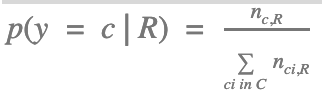
\includegraphics[width=0.7\linewidth]{480.jpeg}
	\end{figure}
	ovvero prendiamo le singole distribuzioni delle varie classi e le dividiamo per la somma completa delle distribuzioni all’interno di quella regione.
	È importante notare che la somma di tutte queste probabilità sarà sempre uguale a 1.

		\item Alla fine all’istanza x viene assegnata la classe che ha la probabilità più alta.
		Un esempio: siamo in una regione con 10 istanze, 2 sono verdi e 8 blu, quindi calcoliamo la distribuzione e vediamo che Nr = (verde = 2, blu =8).
		Ora calcoliamo la probabilità che una nuova istanza sia classificata come verde: 2/10 = 0.2 e la probabilità che sia classificata come blu: 8/10 = 0.8.
		Quindi classifichiamo la nuova istanza come blu.
		
		\end{itemize} 

		\section{Creare il decision Tree ottimo}

		Per la creazione di un decision tree possiamo suddividere il processo in due fasi, learning phase e test phase. Partendo con una certa quantità di dati dobbiamo dividere questi dati nei soliti set: 
		\begin{itemize}
			\item Training Set
			\item Validation Set
			\item Test Set
			
			\end{itemize} 
		
			Una prima idea che potremmo avere per generare il miglior decision tree possibile è quella di generare tutti i possibili decision tree (in base alle varie feature che abbiamo a disposizione e ai possibili valori). Quindi nella fase di training generiamo tutti gli alberi e poi nella fase validation li proviamo tutti fino e trovo il migliore ovvero quello che generalizza meglio.
Questa idea è del tutto impossibile da realizzare ed è anche inefficiente perchè dovremmo generare un numero decisamente troppo alto di alberi.
Ad esempio, consideriamo solamente il nodo root, quindi solo la prima feature che vogliamo prendere in considerazione e i valori. Se avessimo solamente due feature e ogni feature avesse 300 possibili valori numeri, avremo 299 possibili threshold per fare lo split. Quindi in pratica avrei 2*299 = 598 possibilità solamente per il nodo root (la formula generale è D*(N-1) dove D è il numero di feature e N è il numero di possibili valori da testare).
Ovviamente questo numero di possibili alberi da testare aumenta a mano a mano che scendiamo di più nell’albero.

\subsubsection{Algoritmo Greedy}

Trovare il partizionamento ottimo per l’albero di decisione è un problama NP-completo e quindi si utilizzano delle euristiche per trovare un albero che pur non essendo l’ottimo è comunque valido da poter essere utilizzato.
L’algortimo che viene usato per trovare il migliore split è greedy, si guarda al dataset che abbiamo a disposizione e poi si prende di volta in volta lo split che mi permette di avere la migliore separazione dei dati. 
Per capire se devo continuare a splittare un certo nodo oppure no ci sono varie possibili euristiche:
Quello che guadagno con lo split è troppo poco?
Vado oltre l’altezza massima dell’albero che voglio avere?
La distribuzione delle classi nelle foglie è abbastanza omogenea? (Quindi i figli sono abbastanza puri)
Il numero degli esempi che rimangono nelle foglie è troppo piccolo?


\chapter{Lezione 3 - Probabilistic Inference}

\section{Refresh: } Differenza tra discrete random variable e continuous random variable:
\begin{itemize}
\item Una variabile F si dice discrete random variable quando può assumere solamente una quantità finita di possibili valori.
\item Una variabile F si dice continuous random variable quando può assumere un qualsiasi valore all'interno di un intervallo di numeri.
\end{itemize}

In statistica si distinguono probability mass function (PMF) e probability density function (PDF):
\begin{itemize}
\item Probability mass function: è una funzione che mi dice la probabilità che una certa variabile sia esattamente uguale ad un certo valore. Abbiamo
la PMF solamente se la variabile che consideriamo è discreta. Ad esempio se abbiamo una variabile che può assumere solamente 2 valori allora possiamo
modellare la distribuzione usando la PMF indicando P(F=f). Questa variabile F potrà assumere solamente due valori, 1 o 0. Se vogliamo valutare la PMF
calcoliamo la probabilità di avere P(F=1) o P(F=0). È importante notare che se la variabile è discreta non ha la PDF.
\item Probability density function: è una funzione il cui valore in ogni punto del sample space mi indica la likelihood che il valore della random
variable possa essere uguale a quel valore. La PDF viene usata per specificare la probabilità che una variabile random cada all'interno di un
particolare range. La PDF deve essere integrata sul suo intervallo per arrivare ad avere una probabilità. Questo intervallo su cui calcolare la
probabilità potrebbe essere l'intervallo intero o anche parte dell'intervallo se consideriamo la probabilità di finire in un range. Il calcolo
dell'integrale equivale a trovare l'area sotto la curva. L'area sotto tutta la curva deve essere uguale a 1. Quindi nell'esempio precedente abbiamo la
variabile discreta F che può assumere solamente due valori 1 e 0, possiamo specificare la probabilità che questa variabile assuma uno di questi due
valori usando una variabile che è continua e che chiamiamo $\Theta \in [0,1]$. $\Theta$ è continua perchè può assumere qualsiasi valori nel range e la
distribuzione di F dipende da $\Theta$ quindi possiamo scrivere $P(F=f | \Theta)$. Dato che la variabile $\Theta$ è continua, posso specificarne la
distribuzione utilizzando la PDF. Se la variabile è continua non posso specificare la PMF ma solamente la PDF.
\end{itemize} 

\section{MLE: Ottimizzare la funzione Likelihood}

Consideriamo la situazione in cui abbiamo dei dati, ci possiamo chiedere cosa possiamo imparare da questi dati e come possiamo impararlo. Ad esempio
prendiamo il caso in cui lanciamo per 10 volte una moneta e vogliamo predire il risultato del prossimo lancio.
\begin{figure}[H]
\centering
  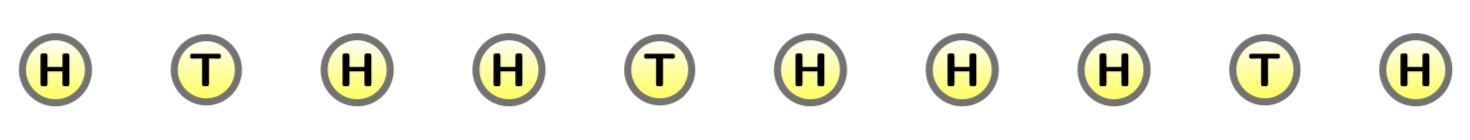
\includegraphics[width=0.8\linewidth]{5.jpeg}
\end{figure}

In questo caso nei precedenti lanci abbiamo 3 volte tail e 7 volte head, un possibile valore per la probabilità del prossimo lancio potrebbe essere
0.5 se la moneta è fair, altrimenti potremmo anche avere 0.3 come probabilità di avere tail perchè head compare 3 volte nei precedenti 10 lanci.

Quello che vogliamo fare è creare un modello per i nostri dati, noi sappiamo che ogni lancio della moneta ha un valore random e quindi anche l'intera
sequenza di valori è del tutto random. Quindi possiamo scrivere la probabilità dell'i-esimo lancio come: 
\begin{figure}[H]
\centering
  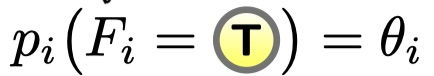
\includegraphics[width=0.3\linewidth]{7.jpeg}
\end{figure}

La variabile $\Theta$ che esprime il valore della probabilità è continua e assume valori all'interno dell'intervallo $[0,1]$ La distribuzione della
variabile discreta F dipende da $\Theta_i$ quindi possiamo scriverla in questo modo notando anche il fatto che possiamo modellare questa probabilità
con la distribuzione di Bernoulli.
\begin{figure}[H]
\centering
  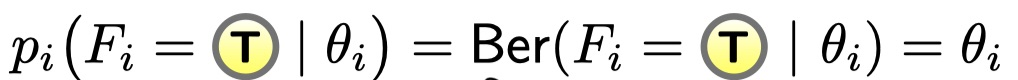
\includegraphics[width=0.6\linewidth]{8.jpeg}
\end{figure}

Possiamo modellarla con Bernoulli perchè siamo in uno spazio binario ovvero la $p_i(F_i = T | \Theta_i)$ ha solamente due possibili valori ovvero
abbiamo che se consideriamo tail avremo probabilità $\Theta_i$ di ottenere tail e poi avremo probabilità $1-\Theta_i$ di avere head. La notazione per
questo tipo di problemi è 

$I[x] = \begin{cases*} 1 & if  x is true  \\
                    0 & if 	x is false \end{cases*}$

Possiamo modellare la nostra sequenza di lanci di monete sulla base di 10 parametri:
\begin{figure}[H]
\centering
  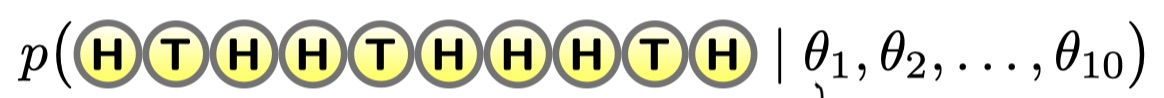
\includegraphics[width=0.8\linewidth]{9.jpeg}
\end{figure}

Noi data l'osservazione di questa specifica sequenza di valori, vogliamo trovare il parametro $\Theta_i$ che massimizza la probabilità di questa
osservazione (massimizza la likelihood). Supponiamo di voler modellare questa probabilità, dobbiamo fare delle assunzioni:
\begin{itemize}
\item La prima assunzione che facciamo è che i lanci delle monete sono indipendenti l'uno dall'altro, questo vuol dire che al momento i non mi
interessa dei risultati dei precedenti lanci. Questo mi permette di esprimere la probabilità come un prodotto delle singole probabilità, qui stiamo
indicando che $F1,...,F10$ sono variabili indipendenti. 
\begin{figure}[H]
\centering
  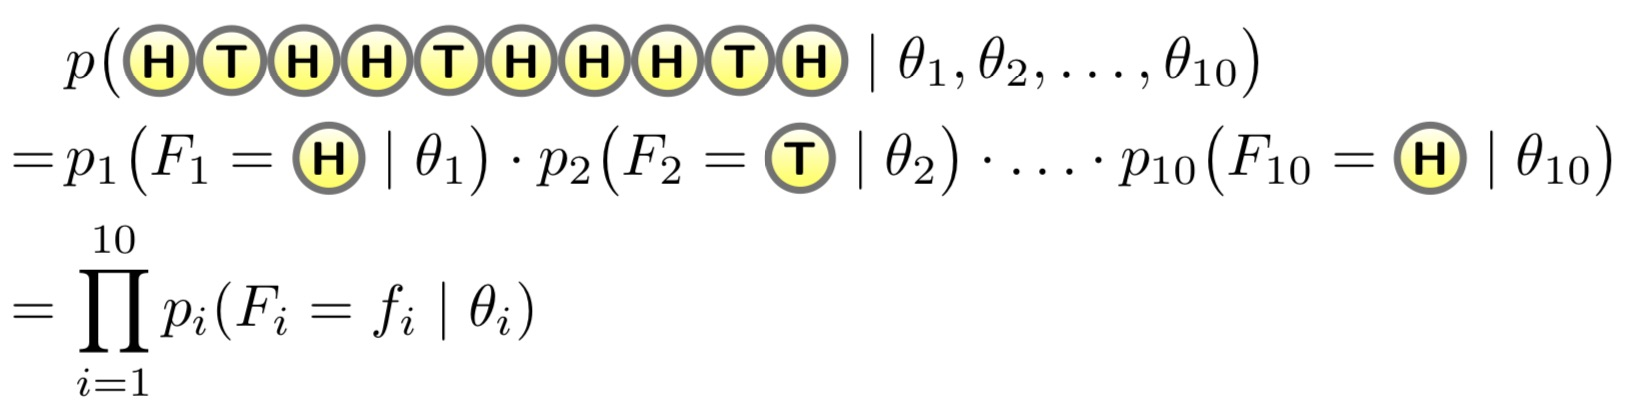
\includegraphics[width=0.88\linewidth]{11.jpeg}
\end{figure}
\item La seconda assunzione che facciamo è che la distribuzione dei lanci è sempre la stessa, quindi la $\Theta_i$ in realtà non varia da un lancio
all'altro ma è un qualcosa di costante, quindi possiamo considerare solamente $\Theta$ in ognuna delle probabilità.
\begin{figure}[H]
\centering
  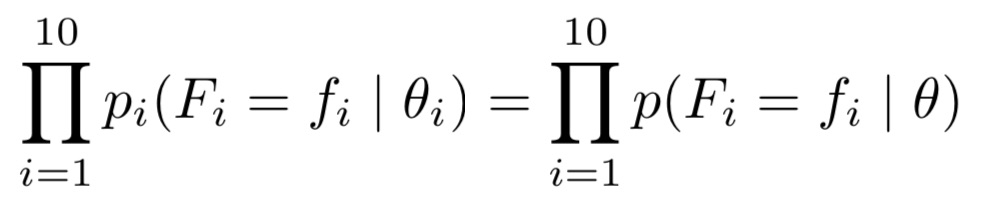
\includegraphics[width=0.5\linewidth]{13.jpeg}
\end{figure}
\end{itemize}
Quindi in pratica stiamo assumento che i 10 lanci siano sia indipendenti sia equamente distribuiti. Questo mi permette di considerare la variabile che
vogliamo predire che sarebbe $\Theta_{11}$ come una semplice $\Theta$ identica a tutte le altre. A questo punto possiamo scrivere la probabilità dei
dati che abbiamo osservato:
\begin{figure}[H]
\centering
  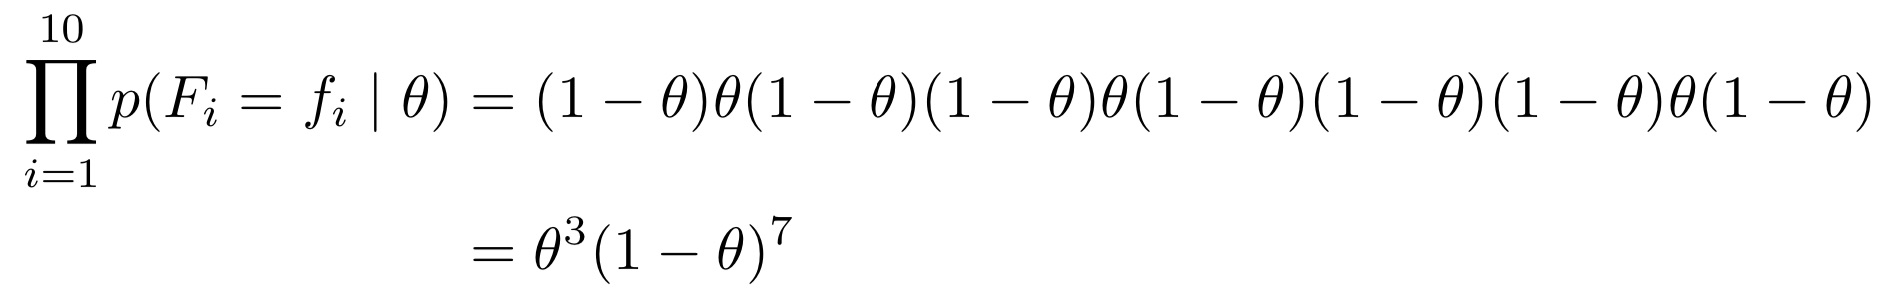
\includegraphics[width=0.80\linewidth]{14.jpeg}
\end{figure}
Questa dipende da $\Theta$ e mettiamo $\Theta$ quando abbiamo tail mentre $1-\Theta$ quando abbiamo head.\\

\subsection{Ottimizzare}
La probabilità di vedere i nostri dati può essere vista come una funzione: $f(x) = p(D|\Theta)$ dove $D$ sono i nostri dati e $\Theta$ è la
distribuzione. Questa funzione che abbiamo definito è la likelihood di $\Theta$, questa non è una distribuzione della probabilità di $\Theta$ ma è la
distribuzione della probabilità di $D$. Il nostro obiettivo è trovare la $\Theta$ che mi massimizza questa funzione di likelihood ovvero vogliamo
trovare la $\Theta_{MLE}$ dove MLE = Maximum likelihood estimation.
\begin{figure}[H]
\centering
  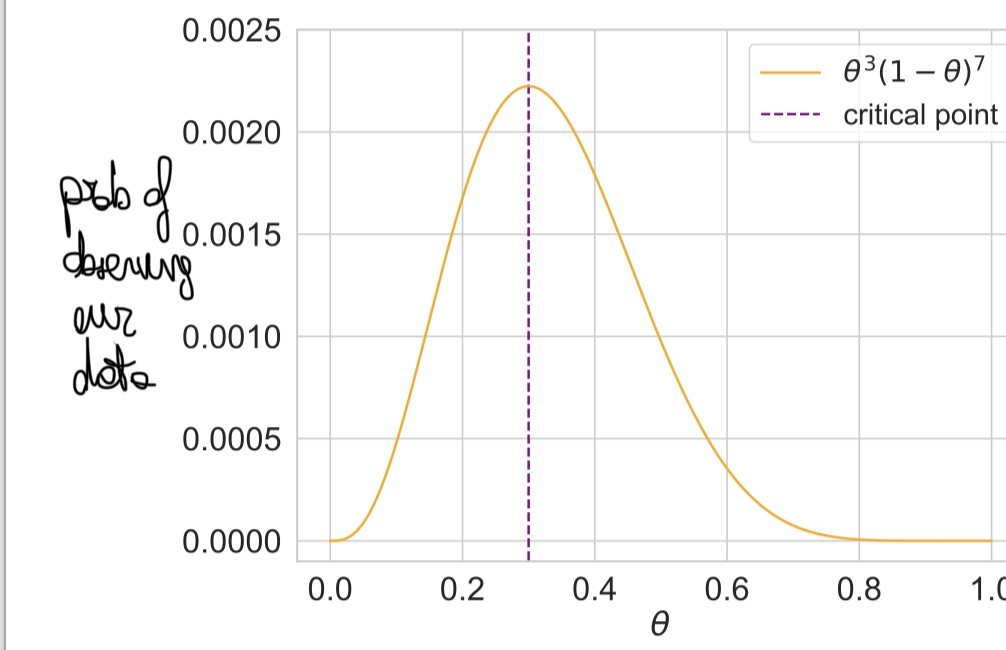
\includegraphics[width=0.7\linewidth]{15.jpeg}
\end{figure}

Nel grafico possiamo vedere chiaramente i possibili valori che assume $\Theta$ e come varia la probabilità di osservare i nostri dati, noi siamo
interessati al valore di $\Theta$ che massimizza questa probabilità.

Come facciamo a massimizzare $f(x) = p(D|\Theta)$ che in questo caso sarebbe $f(x) = \Theta^3(1-\Theta^87)$? Calcoliamo la derivata di questa funzione
e la poniamo uguale a 0, poi prendiamo i punti in cui la derivata è 0 e calcoliamo la derivata seconda vedendo come si comporta nei punti critici
evidenziati in precedenza.

Massimizzare una funzione di questo genere può essere difficoltoso e quindi possiamo sfruttare una proprietà della funzione del logaritmo per
semplificare i calcoli. 
\begin{figure}[H]
\centering
  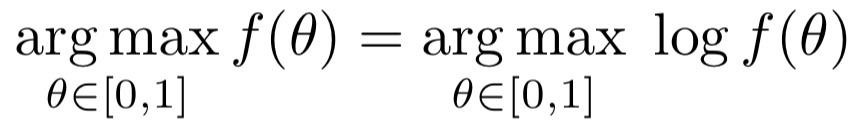
\includegraphics[width=0.5\linewidth]{23.jpeg}
\end{figure}
La funzione logaritmica infatti è monotona quindi vuol dire che i massimi della funzione originale sono gli stessi quando applichiamo il logaritmo
alla funzione originale: $f(x*) > f(y) \forall y \implies log(f(x*))> log(f(y))  \forall y $. Possiamo vedere questa proprietà nel seguente grafico:
\begin{figure}[H]
\centering
  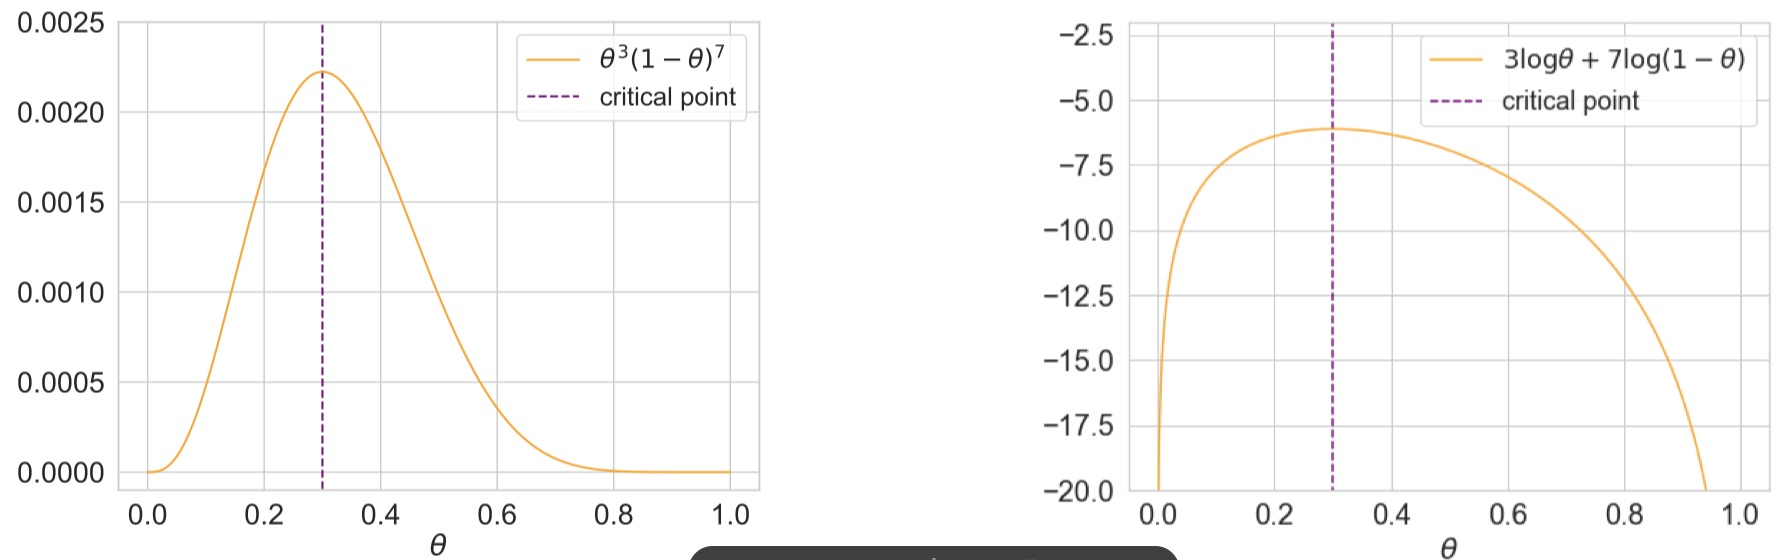
\includegraphics[width=\linewidth]{22.jpeg}
\end{figure}

Vediamo che il massimo della funzione è sempre nello stesso punto anche se applichiamo il logaritmo. In questo caso applicando il logaritmo la
funzione da massimizzare diventa $3Log\Theta + 7Log(1-\Theta)$, quindi molto più semplice da calcolare.

Possiamo quindi massimizzare la funzione e in questo caso otteniamo la nostra $\Theta_{MLE} = \frac{|T|}{|T|+|H|}$, questo valore lo possiamo
utilizzare per stimare la probabilità che il prossimo lancio sia head o tail:
\begin{figure}[H]
\centering
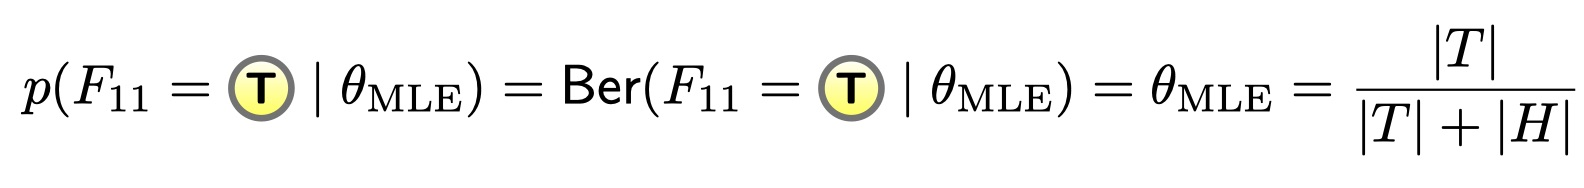
\includegraphics[width=0.7\linewidth]{24.jpeg}
\end{figure}
Tutto questo mi giustifica il fatto che la probabilità di avere $\Theta_{11} = T$ possa essere 0.3.

\subsection{Problemi della MLE}

Per capire il problema principale dell'MLE consideriamo un altro esempio:
\begin{figure}[H]
\centering
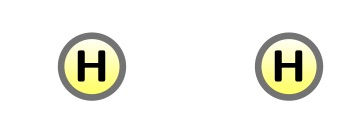
\includegraphics[width=0.3\linewidth]{27.jpeg}
\end{figure}
Abbiamo la seguente sequenza di lanci di monete, in questo caso però c'è sempre Head e mai tail quindi vuol dire che la f che dovremmo massimizzare
sarà $f(x)=(1-\Theta)^2$. Se massimizzo questa funzione vediamo che il valore massimo ce l'abbiamo con $\Theta_{MLE} = 0$ e questo è un problema
perchè stiamo dicendo che non potremo mai vedere tail. Chiaramente il problema dell'MLE è che va in overfitting perchè non considera delle conoscenze
pregresse che un umano può avere, come ad esempio il fatto che ogni volta c'è il 50\% di probabilità di fare tail e il 50\% di fare head. Quindi per
risolvere questo problema si dovrebbe trovare un modo per incorporare all'interno del modello questa conoscenza pregressa per evitare l'overfitting.


\section{Bayesian Inference}

Nel caso della MLE abbiamo una $\Theta$ che dipende dai dati che abbiamo, noi ora vorremmo rappresentare la distribuzione di $\Theta$ basandoci sulle
nostre idee conoscenze riguardo al dominio di cui si sta parlando (ad esempio le monete in questo caso). La distribuzione di $\Theta$ quindi deve
essere una prior distribution e deve rappresentare quello che conosciamo prima di vedere i dati, ci sono dei vincoli che devono essere rispettati:
\begin{itemize}
\item La distribuzione $p(\Theta)$ deve essere del tutto indipendente dai dati
\item $p(\Theta)>0 \ \forall \ \Theta$ In questo caso i possibili valori di $\Theta$ sono 0 e 1.
\item L'integrale della distribuzione deve essere uguale a 1 (l'area sotto la curva deve essere 1). $\int p(\Theta) d\Theta = 1$
\end{itemize}

Partendo da queste regole possiamo provare a formulare un modello ovvero possiamo pensare a varie possibili distribuzioni per la $	\Theta$ calcolando
quindi la prior probability $p(\Theta)$.


\begin{figure}[H]
\centering
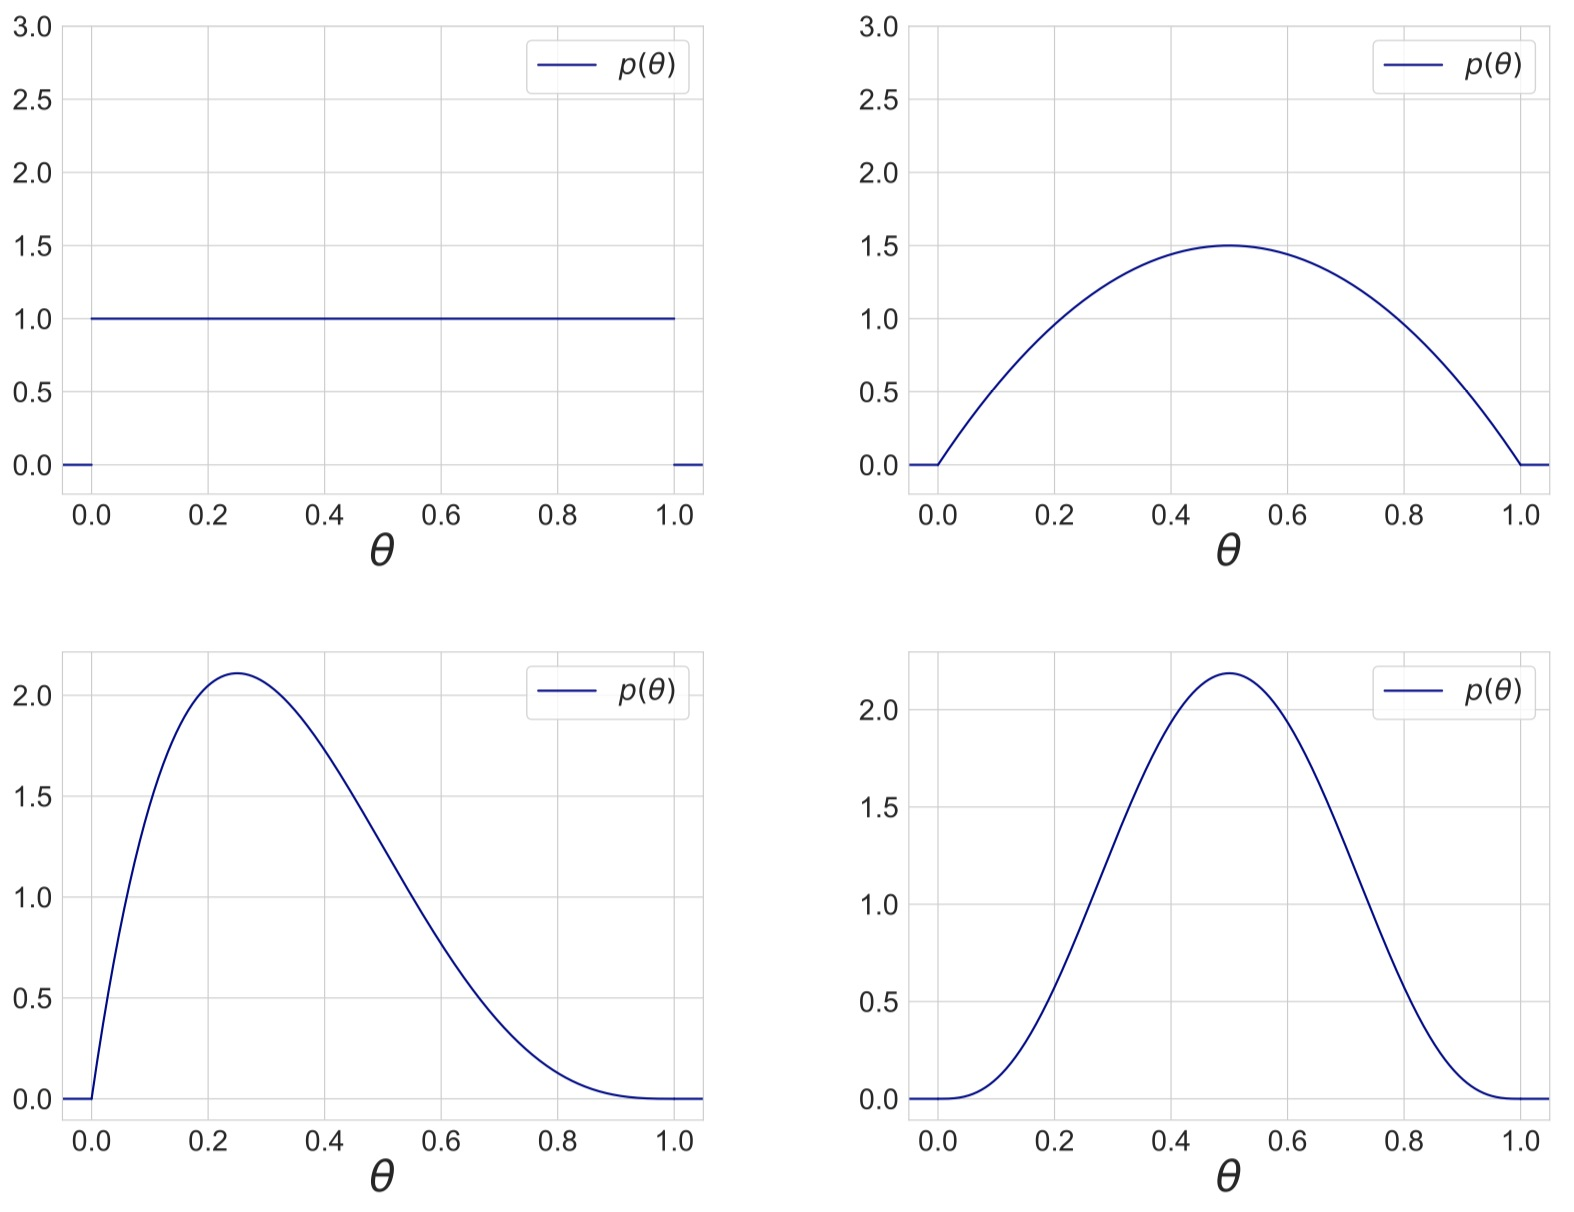
\includegraphics[width=0.7\linewidth]{29.jpeg}
\end{figure}

Alcuni esempi:
\begin{itemize}
\item Nel primo esempio abbiamo una distribuzione uniforme quindi vuol dire che abbiamo sempre la stessa probabilità di ottenere un certo risultato.
\item Nel secondo esempio abbiamo che la probability density function è più spostata verso il centro e quindi possiamo dire che abbiamo una preferenza
per i valori che stanno al centro di questa curva. Questo lo possiamo anche trasformare in una probabilità se consideriamo ad esempio i valori di
$\Theta$ compresi tra 0.4 e 0.6, calcolando l'integrale infatti riusciamo a vedere che la probabilità di avere un valore di $\Theta$ in questo
intervallo è maggiore degli altri.
\item Nel quarto grafico questa preferenza verso il centro è ancora più netta.
\end{itemize}

Ci sono alcuni cose che vanno sottolineate:
\begin{itemize}
\item $\Theta$ è una variabile continua
\item È importante considerare che l'area sotto la curva deve essere sempre uguale a 1 e questo lo dimostriamo se calcoliamo l'integrale della curva
dal punto in cui inizia al punto in cui finisce.
\item La densità (quanto va in alto la curva) può essere maggiore di 1 perchè non è una probabilità. Qua abbiamo la probability density function e non
la probability mass function.
\end{itemize}


\subsection{Bayes Formula}

Quello che vorremmo fare è aggiornare la distribuzione della $\Theta$ una volta che abbiamo osservato i dati. Quindi per questo utilizziamo la formula
di Bayes che mi permette di calcolare la posterior probability.

\begin{figure}[H]
\centering
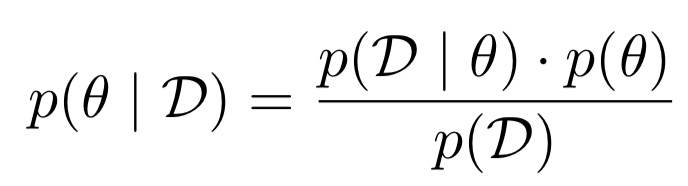
\includegraphics[width=0.4\linewidth]{30.jpeg}
\end{figure}

Analizziamo la formula:
\begin{itemize}
\item $P(\Theta | D)$ è la posterior distribution, questa distribuzione mi permette di capire ciò che conosciamo della distribuzione $\Theta$ dopo che
ho osservato i dati $D$.
\item $P(D|\Theta)$ è la likelihood
\item $P(\Theta)$ èa la prior distribution ovvero le nostre conoscenze prima di osservare i dati
\item $p(D)$ è una costante che viene usata per normalizzare e fa in modo che la posterior distribution sia integrata ad 1. Questa costante la
esprimiamo come: $p(D) = \int p(D,\Theta) d\Theta = \int p(D|\Theta) p(\Theta) d\Theta$. In pratica stiamo calcolando l'integrale della distribuzione
non normalizzata $p(D|\Theta) p(\Theta)$.
\end{itemize}

Nell'esempio si vede bene come viene modificata la distribuzione della $\Theta$ in base ai dati che vediamo:

\begin{figure}[H]
\centering
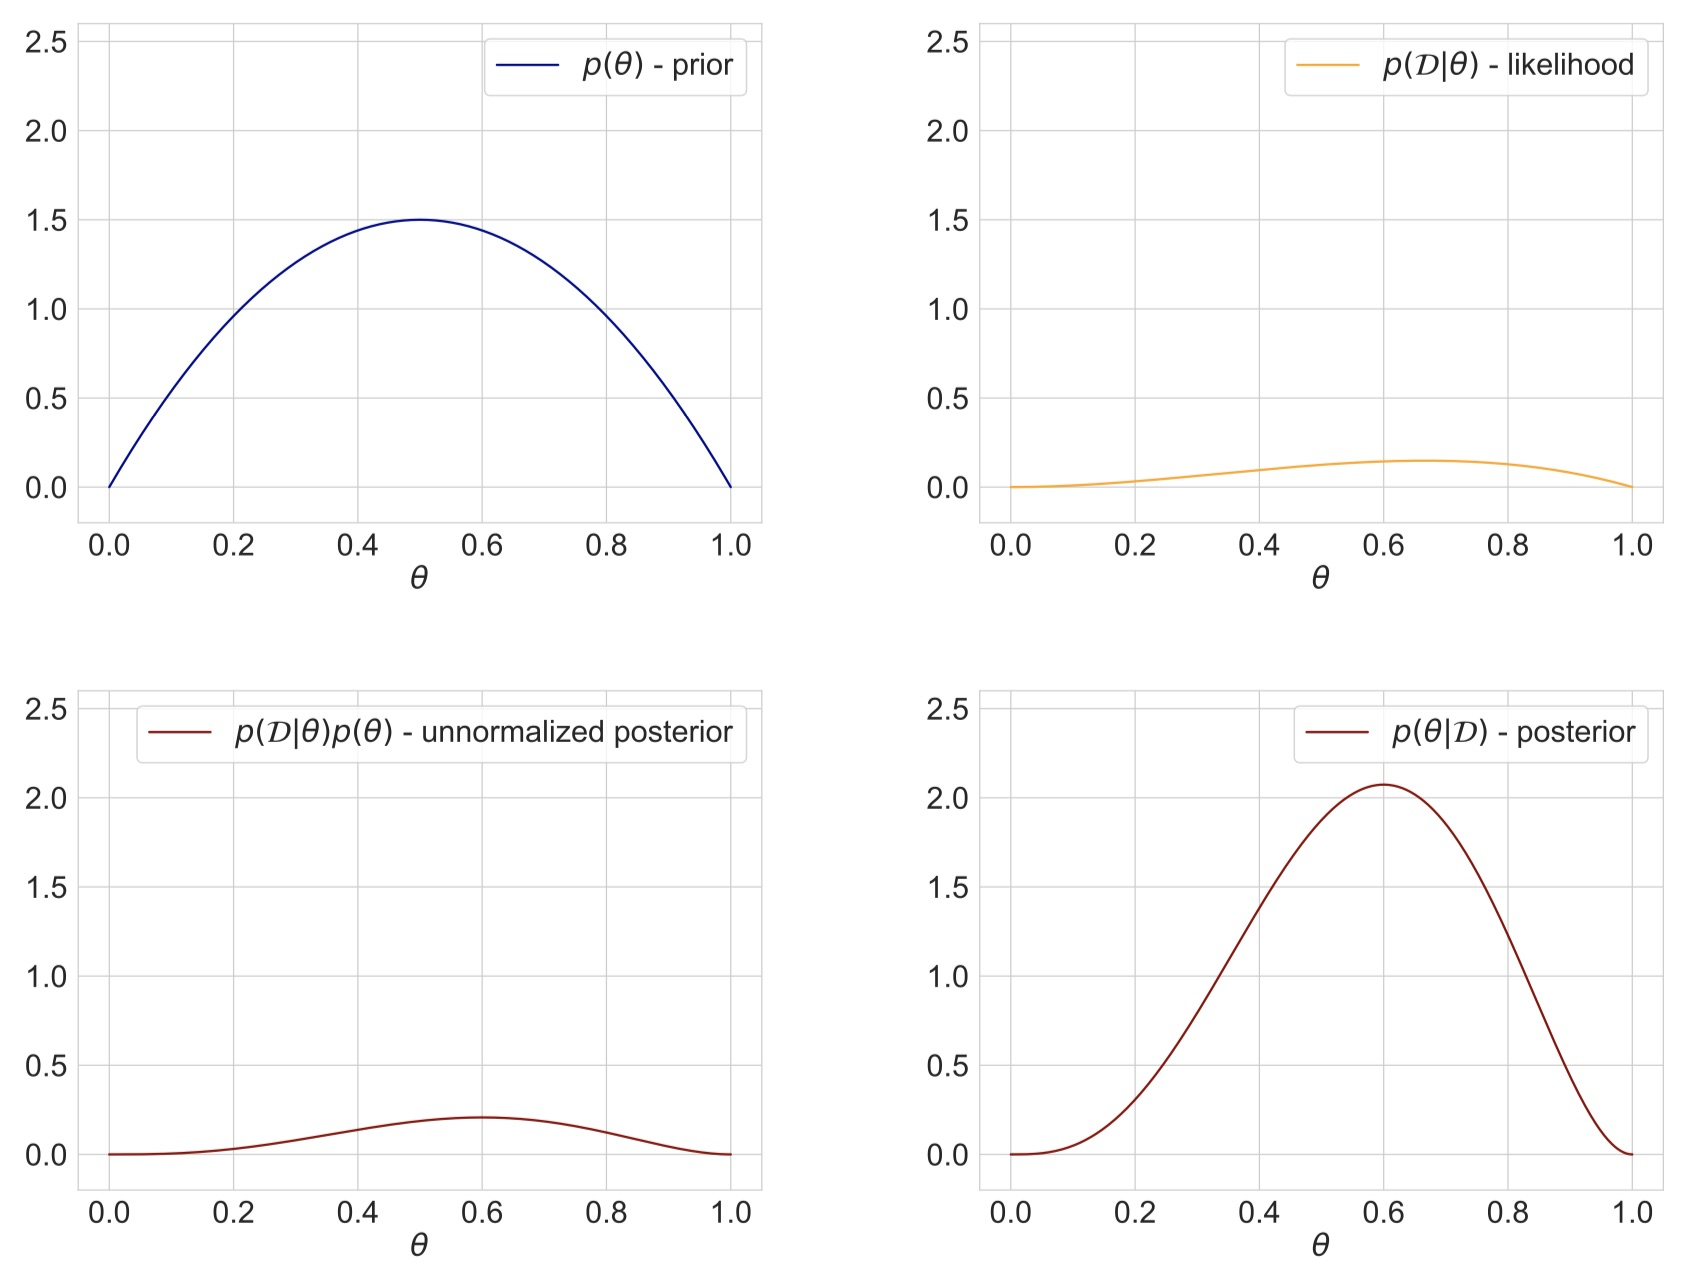
\includegraphics[width=0.7\linewidth]{31.jpeg}
\end{figure}

\begin{itemize}
\item Nel primo grafico abbiamo la prior distribution $p(\Theta)$
\item Nel secondo grafico abbiamo la distribuzione della likelihood $p(D|\Theta)$
\item Nel terzo grafico (ottenuto moltiplicando $p(\Theta)$ con $p(D|\Theta)$) abbiamo la posterior distribution non normalizzata. Ora calcoliamo
l'integrale dell'area sotto questa curva per ottenere $p(d)$.
\item Nell'ultimo grafico viene fatta la normalizzazione e otteniamo la posterior distribution che è diversa rispetto alla nostra idea iniziale di
questa distribuzione.
\end{itemize}

Più dati osserviamo e più riusciamo ad aumentare la confidence, nel seguente grafico possiamo notare come aggiungendo dati ci si distacchi dalla prior
distribution andando ad ottenere una posterior distribution che è sempre più simile alla likelihood. In realtà in questo caso la likelihood è stata
scalata per fare in modo che potesse notarsi perchè di norma la curva è più bassa.

\begin{figure}[H]
\centering
\includegraphics[width=0.7\linewidth]{32.jpeg}
\end{figure}

Ovviamente più la nostra previsione della distribuzone $\Theta$ è accurata e meno tempo ci vuole per convergere alla posterior probability.

\subsection{Problema}

C'è un caso in cui potremmo avere un problema, se la prior distribution è 0 per un qualche valore di $\Theta$ vuol dire che anche la posterior
distribution sarà 0 indipendentemente dal valore della likelihood.

\section{MAP: Maximum A Posterior Estimation}

Abbiamo visto come calcolare la $\Theta_{MLE}$ e come calcolare la posterior distribution, nel caso della $\Theta_{MLE}$ abbiamo il problema
dell'overfitting e il fatto che non considera la nostra conoscenza pregressa dell'argomento che stiamo considerando. Invece di provare a massimizzare
la likelihood allora potrebbe essere una buona idea provare a massimizzare la posterior distribution, questa idea è chiamata MAP (Maximum a posteriori
estimation). La formula che possiamo utilizzare per fare questa ottimizzazione è la seguente: 
\begin{equation}
	\Theta_{MAP} = argmax_{\Theta} p(\Theta | D) = argmax_{\Theta} \frac{p(D|\Theta)p(\Theta)}{p(D)}
\end{equation}

In questa formula possiamo anche non considerare $\frac{1}{p(D)}$ perchè è una costante che non dipende da $\Theta$. Questo possiamo farlo perchè
$argmax_{\Theta} f(\Theta) = argmax_{\Theta} C *f(\Theta)$ dove C è una costante. Quindi la nostra formula diventa:
\begin{equation}
	\Theta_{MAP} = argmax_{\Theta} \ p(D|\Theta)p(\Theta)
\end{equation}

Ora il problema è la scelta della prior distribution $p(\Theta)$.

\subsection{Scegliere la prior distribution}

Solitamente la scelta della prior distribution ricade su una "Beta distribution" perchè rende più semplici i calcoli successivi.
\begin{figure}[H]
\centering
\includegraphics[width=0.7\linewidth]{34.jpeg}
\end{figure}

Questa beta distribution dipende da due parametri che sono $a>0$ e $b>0$.

Nella formula della beta distribution abbiamo anche la gamma function che in questo caso viene utilizzata per normalizzare la distribuzione e fare in
modo che l'integrale sia uguale a 1.

\begin{figure}[H]
\centering
\includegraphics[width=0.17\linewidth]{35.jpeg}
\end{figure}

A seconda del valore che assumono i parametri avremo una differente curva della distribuzione.
\begin{figure}[H]
\centering
\includegraphics[width=0.7\linewidth]{36.jpeg}
\end{figure}

In particolare nel grafico abbiamo 4 possibili combinazioni per a e b e possiamo dire che l'ultima curva con $a=0.1$ e $b=0.1$ ci troviamo in una
situazione in cui è più alta la probabilità che $\Theta$ sia 0 o 1. Al contrario, nei casi in cui a e b sono $> 1$ la distribuzione ha una curva che
va in senso opposto, in ogni caso abbiamo solamente un massimo e non ci troviamo ad avere una curva con tanti massimi locali. Avere questi parametri a
e b fa si che la posterior distribution non sia solamente dipendente da $\Theta$ ma anche da a e da b.

\subsection{Calcolare la MAP}


Per calcolare la MAP notiamo prima che:
\begin{itemize}


\item Scriviamo $f(x) \propto g(x)$ ovvero che $f(x)$ è proporzionale a $g(x)$ se esiste una $c$ tale che $f(x) = c*g(x)$. La costante c è
indipendente dalla funzione. Un esempio è $5x^2 \propto x^2$.
\item Nella notazione della posterior probability non scriviamo a e b ma in realtà dipende anche da queste due variabili.
\end{itemize}

Consideriamo ora la formula della posterior probability, questa è proporzionale alla formula in cui non dividiamo per $p(d)$ perchè è una costante. 

\begin{figure}[H]
\centering
\includegraphics[width=0.3\linewidth]{37.jpeg}
\end{figure}

Sapendo che valgono le seguenti uguaglianze:
\begin{figure}[H]
\centering
\includegraphics[width=0.7\linewidth]{38.jpeg}
\end{figure}

Possiamo dire che:

\begin{figure}[H]
\centering
\includegraphics[width=0.7\linewidth]{39.jpeg}
\end{figure}

Nel primo passaggio andiamo semplicemente a sostituire i valori con quelli mostrati prima, il secondo passaggio è giustificato dal fatto che la gamma
function che usiamo per normalizzare non dipende da $\Theta$ e quindi possiamo tranquillamente non considerarla. Sempre nel secondo passaggio andiamo
anche a combinare gli esponenti. \\
\textbf{Come scegliamo a e b?}

Nel caso dell'esempio del coin tossing, se la moneta è fair possiamo scegliere due valori che sono simili tra loro. Se non abbiamo una conoscenza
pregressa invece scegliamo a e b in modo da ottenere una distribuzione uniforme.


Una volta che abbiamo ottenuto la formula della $\Theta_{MAP}$ vogliamo massimizzare questa equazione.
\begin{figure}[H]
\centering
\includegraphics[width=0.5\linewidth]{40.jpeg}
\end{figure}
Anche in questo caso possiamo usare il trucco del logaritmo per fare in modo che il calcolo diventi più semplice e quindi otteniamo:
\begin{figure}[H]
\centering
\includegraphics[width=0.7\linewidth]{41.jpeg}
\end{figure}

Alla fine la $\Theta_{MAP}$ diventa uguale a:
\begin{figure}[H]
\centering
\includegraphics[width=0.4\linewidth]{42.jpeg}
\end{figure}

Data questa ultima equazione possiamo fare un confronto con l'equazione della $\Theta_{MLE}$, qua noi abbiamo i parametri a e b che vengono utilizzati
per controllare l'overfitting e per evitarlo. \\
Se consideriamo infatti la formula $\Theta_{MLE} = \frac{|T|}{|T|+|H|}$ e i seguenti dati:
\begin{itemize}
	\item $D = \{H, H\}$ 
	\item $a=b=5$
	\item $|H| = 2 \ e\ |T| = 0$
\end{itemize}

E vogliamo stimare la probabilià di ottenere T al prossimo lancio otteniamo i seguenti valori:
\begin{itemize}
\item $\Theta_{MLE} = 0$
\item $\Theta_{MAP} = \frac{0+5-1}{2+0+5+5-2} = \frac{4}{10} = 0.4$
\end{itemize}

Quindi con la $\Theta_{MAP}$ riesco ad evitare l'overfitting, con la $\Theta_{MLE}$ invece qua dico che non ho probabilità di ottenere T al prossimo
lancio.

\section{Estimate the posterior distribution}

Fino ad ora abbiamo visto come calcolare la $\Theta_{MAP}$ che, se consideriamo il grafico, rappresenta la moda della distribuzione ovvero il punto in
cui la densità è più alta. Se vogliamo rispondere ad altre domande (ad esempio quanto è sicura la nostra stima o quale è la probabilità che $\Theta$
sia in un certo intervallo) però dobbiamo considerare non solo la moda ma tutta la distribuzione $p(\Theta | D)$.

Per calcolare la posterior distribution reale dobbiamo essere capaci di calcolare la costante che si usa per la normalizzazione perchè fino ad ora
avevamo calcolato sfruttando il fatto che la formula è proporzionale:

\begin{figure}[H]
\centering
\includegraphics[width=0.7\linewidth]{45.jpeg}
\end{figure}

Per trovare il valore della variabile di normalizzazione ci sono due strade:
\begin{itemize}
\item La prima strada è quella più complessa e consiste nel risolvere l'integrale $$\int_0^1 \Theta^{|T|+a-1} (1-\Theta)^{|H|+b-1} d\Theta$$ Dato il
risultato C di questo integrale possiamo dire che la costante di normalizzazione sarà $\frac{1}{C}$, questo perchè l'integrale della posterior
probability deve essere uguale a 1 quindi avremmo: $$\int_0^1 Z * \Theta^{|T|+a-1} (1-\Theta)^{|H|+b-1} d\Theta = 1$$ $$Z*\int_0^1 \Theta^{|T|+a-1}
(1-\Theta)^{|H|+b-1} d\Theta = 1$$ $$Z*C = 1 \implies Z = \frac{1}{Z} $$	Questa strada però è complessa perchè si deve calcolare l'integrale.
\item Possiamo fare un po' di pattern matching e notare che la posterior probability non normalizzata somiglia alla posterior distribution function
della beta distribution
$$Beta(\Theta | \alpha, \beta) = \frac{\Gamma(\alpha + \beta)}{\Gamma(\alpha)\Gamma(\beta)}\Theta^{\alpha-1}(1-\Theta)^{\beta-1}$$
\end{itemize}

La seconda soluzione è quella che viene normalmente adottata, possiamo derivare in questo modo la posterior distribution completa facendo i seguenti
calcoli: Noi partiamo con la posterior distribution non normalizzata:

$$p(\Theta | D) = \Theta^{|T| +\alpha-1}(1-\Theta)^{|H|-\beta-1}$$

Calcoliamo l'integrale della beta distribution e lo uguagliamo a 1:
$$\int_0^1\frac{\Gamma(\alpha + \beta)}{\Gamma(\alpha)\Gamma(\beta)}\Theta^{\alpha-1}(1-\Theta)^{\beta-1} = 1$$
$$= \frac{\Gamma(\alpha + \beta)}{\Gamma(\alpha)\Gamma(\beta)}\int_0^1\Theta^{\alpha-1}(1-\Theta)^{\beta-1} = 1$$
$$= \int_0^1\Theta^{\alpha-1}(1-\Theta)^{\beta-1} = \frac{\Gamma(\alpha)\Gamma(\beta)}{\Gamma(\alpha + \beta)}$$

Per se sostituiamo $\alpha = |T|+a$ e $\beta = |H|+b$ si ottiene esattamente la posterior distribution non normalizzata. Questo quindi ci fa capire
che il coefficiente di normalizzazione che vogliamo usare per il calcolo della posterior distribution sarà:
$$\frac{\Gamma(|T|+a + |H|+b)}{\Gamma(|T|+a)\Gamma(|H|+b)}$$ Da qui possiamo concludere che la posterior distribution è a sua volta (così come la
prior distribution) una beta distribution (la prior l'avevamo scelta noi perchè ci sarebbe poi stato comodo per i calcoli). Quindi: $$p(\Theta|D) =
Beta(\Theta|\ a+|T|, b+|H|)$$

Possiamo notare una cosa, la posterior distribution, così come la prior distribution sono beta distribution e sono anche simili perchè la priori è
$$p(\Theta) = Beta(\Theta|\ a, b|)$$ Questo ce lo spieghiamo se consideriamo questa regola delle probabilità:\\
\textit{Nella teoria Bayesiana delle probabilità, se la posterior distribution e la prior distribution hanno la stessa famiglia di distribuzione
allora prior e posterior sono chiamate conjugate distribution e la prior è conjugate prior della likelihood}.

Quindi, in questo caso abbiamo la prior distribution che è conjugate prior della likelihood e questo vuol dire che $a$ e $b$ possono essere
interpretate come numero di tail e head viste nel passato.

Quando poi abbiamo altri dati che possiamo considerare, questa posterior distribution diventa la prior distribution dell'iterazione successiva.

\subsection{Vantaggi del calcolo completo della posterior distribution}

Calcolare la posterior distribution completa ci permette quindi di rispondere a più domande rispetto ad avere solamente la posterior probability:
\begin{itemize}
\item Possiamo trovare il range tale che $P(\Theta \in (\Theta_1,\Theta_2)|D) = 95\%$.
\item Possiamo calcolare la varianza della distribuzione.
\item Possiamo calcolare l'expected value.
\end{itemize}

\subsubsection{Soluzioni viste fino ad ora}

Fino ad ora abbiamo visto le seguenti soluzioni:
\begin{figure}[H]
\centering
\includegraphics[width=0.5\linewidth]{46.jpeg}
\end{figure}

Tutte queste soluzioni sono legate l'una all'altra:
\begin{itemize}
\item Data la posterior distribution $p(\Theta|D) = Beta(\Theta|\ a+|T|, b+|H|)$ e sapendo che la moda della beta distribution è $\frac{\alpha -1
}{\alpha + \beta - 2}$ vediamo che la $\Theta_{MAP}$ è la moda della posterior distribution (poniamo $\alpha=|T|+a$ e $\beta=|H|+b$):
$$\Theta_{MAP}=\frac{|T|+a-1}{|H|+|T|+a+b-2}$$
\item Se scegliamo una distribuzione uniforme per la prior distribution ($a=1$ e $b=1$) otteniamo la $\Theta_{MLE}$:
$$\Theta_{MLE}=\frac{|T|+1-1}{|H|+|T|+1+1-2} = \frac{|T|}{|T|+|H|}$$
\end{itemize}
Questi risultati sono una conseguenza del fatto che scegliamo un conjugate prior.

\subsubsection{Visualizzare la posterior distribution}

Sappiamo che partiamo con una prior distribution e vogliamo ottenere una posterior distribution, a mano a mano che abbiamo più dati poi la posterior
distibution diventa più "confidente" e quindi si trova a crescere sempre di più attorno ad un certo punto.
\begin{figure}[H]
\centering
\includegraphics[width=0.7\linewidth]{47.jpeg}
\end{figure}


\section{Previsione del prossimo lancio}

Abbiamo tutta la posterior probability $P(\Theta | D)$ e vogliamo predire la probabilità che la prossima moneta che lancio sia tail dati i dati che
abbiamo a disposizione e la prior distribution. Quello che vogliamo calcolare quindi è la \textbf{posterior predictive distribution} che è diversa
dalla posterior distribution (che già conosciamo).
 
\begin{figure}[H]
\centering
\includegraphics[width=0.3\linewidth]{48.jpeg}
\end{figure}

Nella formula in figura noi ragioniamo in termini di F, in questo caso è importante capire che questa posterior predictive è una distribuzione di
Bernoulli perchè i valori che possono essere assunti da F sono tail ed Head quindi è una variabile binaria e quindi non può non essere una
distribuzione di Bernoulli.

Quello che cerchiamo è $p(f|D, a,b)$ ovvero la posterior predicted (probabilità che otteniamo un certo tipo di dato), consideriamo la sum rule della
probabilità che mi dice che:
$$p(a|c) = \int p(a,b|c)$$ in questo caso aggiungiamo la variabile b nella joint probability e questo vuol dire che stiamo marginalizzando la b.
Quindi la nostra formula, per la sum rule diventa: $$p(f|D, a,b) = \int_0^1p(f,\Theta|D,a,b)$$

In questo caso noi marginalizziamo la $\Theta$. Ora possiamo riscrivere la formula utilizzando la regola della probabilità condizionale ($P(a,b|c) =
P(a|b,c)P(b|c)$):
$$\int_0^1p(f|\Theta,D,a,b)p(\Theta|D,a,b)$$

Ora possiamo considerare il fatto che le variabili $\Theta,D,a,b$ sono indipendenti e soprattutto possiamo dire che $\Theta$ non è influenzata dalle
altre perchè riguarda il prossimo lancio mentre le altre variabili riguardano le osservazioni precedenti. Quindi la formula diventa:

 $$\int_0^1p(f|\Theta)p(\Theta|D,a,b)$$ In questa formula la seconda parte la conosciamo ed è la posterior distribution mentre la prima parte è la
 likelihood del prossimo lancio. \\
\textbf{Importante:} consideriamo le due parti dell'equazione:
\begin{itemize}
\item La prima parte è la likelihood del prossimo esperimento, nel caso del lancio della moneta anche questa distribuzione è una bernoulliana perchè
anche qua abbiamo solamente due possibili valori per l'outcome.
\item Nella seconda parte della formula abbiamo una posterior distribution e ragioniamo in termini di $\Theta$ quindi abbiamo una beta distribution.
\end{itemize} 


Noi quello che dobbiamo fare è considerare i possibili valori di $\Theta$ e poi per ognuno moltiplichiamo per la posterior distribution che fa da
peso. Un esempio:
\begin{figure}[H]
\centering
\includegraphics[width=0.7\linewidth]{49.jpeg}
\end{figure}

Ora per calcolare la probabilità del prossimo lancio dobbiamo ricordarci queste uguaglianze:

\begin{figure}[H]
\centering
\includegraphics[width=0.8\linewidth]{50.jpeg}
\end{figure}
\begin{figure}[H]
\centering
\includegraphics[width=0.8\linewidth]{51.jpeg}
\end{figure}

Sostituendo e svolgendo alcuni calcoli otteniamo la posterior predictive distribution per il prossimo lancio e possiamo notare che non contiene
$\Theta$ perchè questa variabile l'abbiamo marginalizzata:
\begin{figure}[H]
\centering
\includegraphics[width=0.6\linewidth]{52.jpeg}
\end{figure}

 Tutto questo calcolo viene chiamato "Full Bayesian analysis". \textbf{Importante: }notiamo che la posterior predictive distribution $p(f|D,a,b)$
 segue una distribuzione Bernoulliana, lo capiamo se consideriamo che qua stiamo ragionando in termini di f ovvero di una variabile che può avere
 solamente valore positivo o negativo, quindi è una Bernoulliana. Alcuni esempi dei metodi visti fino a qua a confronto, più dati osserviamo e meno si
 nota la differenza tra i vari metodi:
 
\begin{figure}[H]
\centering
\includegraphics[width=0.7\linewidth]{53.jpeg}
\end{figure}

\chapter{Linear Regression}

Consideriamo il seguente grafico e il seguente problema: abbiamo un datased $D={(x_1,y_1)}_{i=1}^N$.

\begin{figure}[H]
\centering
\includegraphics[width=0.7\linewidth]{64.jpeg}
\end{figure}

Abbiamo delle osservazioni $X = {x_1,...,x_n} \ con x_i \in R^D$ e per ognuna di queste osservazioni abbiamo un target $y = {y_1, ..., y_n}$ con $y_i
\in R$. La $X$ delle osservazioni può essere vista anche come una matrice. Il nostro obiettivo è produrre una previsione $y'$ data la nuova
osservazione $x_{new}$. Per farlo vogliamo trovare una funzione f che mi permette di mappare gli input nei target andando a fittare i dati che abbiamo
a disposizione.

Per un primo esempio scegliamo una $f(x)$ lineare, come ad esempio $$f_w(x_i) = w_0 + w_1x_{i1} + .... + w_nx_{in}$$ Qua abbiamo che ogni dimensione
del vettore x viene moltiplicata per un certo peso $w_i$ e poi viene anche aggiunto del rumore che è rappresentato in questo caso da $w_0$, questo
termine viene chiamato bias o offset term. Più semplicemente possiamo scrivere questa funzione come:
$$f_w(x) = w_0 + w^Tx$$ Se il termine $w_0$ che rappresenta il rumore viene inserito all'interno del vettore $w$ possiamo aggiungere 1 come primo
termine del vettore $x$ e poi ottenere una rappresentazione ancora più compatta: $$f_w(x) = w^Tx$$

Quello che dobbiamo fare è scegliere la migliore $w$ che fitta i nostri dati.

\section{Loss Function}

Per trovare la migliore $w$ dobbiamo considerare una misura di distanza per capire quanto sono differenti la previsione fornita dal nostro modello e
la reale previsione che abbiamo nel nostro dataset. Una possibilità è usare la sum of the squared errors:

\begin{figure}[H]
\centering
\includegraphics[width=0.4\linewidth]{65.jpeg}
\end{figure}

In pratica qua stiamo sommando gli errori che ottengo facendo le previsioni con il mio modello. Questa somma degli errori è sempre positiva e l'unico
caso in cui può essere zero è il caso in cui la funzione che noi usiamo come nostro modello passa per tutti i punti che abbiamo come target.
Graficamente possiamo vederla come la distanza al quadrato tra i punti rossi e la linea blu che è la funzione del nostro modello.

\begin{figure}[H]
\centering
\includegraphics[width=0.3\linewidth]{66.jpeg}
\end{figure}

Dobbiamo trovare la w tale che l'errore sia minore possibile e per farlo dobbiamo minimizzare la funzione dell'errore. La funzione da minimizzare
rispetto alla variabile w è una somma di quadrati dei coefficienti w quindi la derivata sarà lineare rispetto agli elementi di w e quindi in pratica
esiste solamente un singolo minimo $w^*$.
\begin{figure}[H]
\centering
\includegraphics[width=0.4\linewidth]{67.jpeg}
\end{figure}
\begin{figure}[H]
\centering
\includegraphics[width=0.4\linewidth]{68.jpeg}
\end{figure}

Per calcolare la $w$ che minimizza l'errore dobbiamo calcolare il gradiente di questa funzione, quindi in pratica calcoliamo la derivata parziale
rispetto a $w$:

\begin{figure}[H]
\centering
\includegraphics[width=0.6\linewidth]{69.jpeg}
\end{figure}

La derivazione dell'ultimo passaggio è data dal fatto che il primo termine si deriva nel modo seguente: $$(X^TX + (X^TX)^T)w = 2X^TXw$$ Il secondo
termine si deriva: $$-2X^Ty$$ Il terzo è una costante quindi diventa 0. Ora considerando anche la $\frac{1}{2}$ possiamo trovare il risultato finale
che è $$X^TXw-X^Ty$$

Ora che abbiamo il gradiente dobbiamo uguagliarlo a 0 in modo da ottenere la soluzione ottima $w^*$ $$X^TXw-X^Ty=0$$ La soluzione ottima è :

\begin{figure}[H]
\centering
\includegraphics[width=0.3\linewidth]{74.jpeg}
\end{figure}

\section{NonLinear Dependency in data}

Nel precedente esempio abbiamo considerato l'esempio in cui con una funzione lineare riusciamo a fittare i dati e quindi a fare previsione su dati non
ancora visti. Solitamente però i modelli sono più complicati e vorremmo utilizzare delle funzioni che siano più flessibili e capaci di fittare i dati
anche se le dipendenze tra x e y non sono lineari. Un esempio lo vediamo nella figura seguente, i dati (pallini blu) che vediamo sono generati con la
funzione $y_i=sen(2\Pi x_i) + \epsilon_i$ dove la $\epsilon_i$ rappresenta il rumore che vogliamo aggiungere. In particolare questo rumore fa si che i
dati non si trovino perfettamente sulla curva. Quello che si fa è prendere una $x_i$ poi scegliere a caso una $\epsilon_i$ e poi otteniamo la $y_i$, è
importante considerare il fatto che la $\epsilon_i$ segue una distribuzione gaussiana $N(0, \beta^{-1})$

In questo caso i sample non seguono un modello lineare.

\begin{figure}[H]
\centering
\includegraphics[width=0.5\linewidth]{76.jpeg}
\end{figure}

Quello che si fa in questo caso è utilizzare una funzione che non è lineare ma polinomiale perchè è più flessibile. Un esempio di funzione polinomiale
è la seguente

\begin{figure}[H]
\centering
\includegraphics[width=0.7\linewidth]{77.jpeg}
\end{figure}

In questo caso abbiamo che M rappresenta il grado del polinomio e la $w$ rappresenta anche in questo caso il vettore con i coefficienti del polinomio.
Possiamo scrivere questa formula con una rappresentazione più compatta in cui facciamo uso di una funzione chiamata basis function che indichiamo con
$\phi$:
$$w_0+\sum_{j=1}^M w_j\phi_j(x) = w^T\phi(x)$$

La funzione $\phi(x)$ è una funzione che prende il dato x e me lo modifica, in questo caso è definita come $\phi_j(x) = x^j$, nell'ultima
rappresentazione non scriviamo $w_0$ in modo esplicito e quindi dobbiamo considerare anche il fatto che $\phi_j(0)=1$. Ci sono vari modi per definire
la funzione $\phi(x)$ ad esempio anche la Gaussiana o la Sigmoid.

Consideriamo ora un caso particolare, ora la x che stiamo considerando come input non è solamente uno scalare ma è un vettore di dimensione d e la
funzione che mi trasforma i dati ora mi prende questo vettore di dimensione d e me lo trasforma in uno scalare: $\phi: R^d->R$.

La formula delle previsioni è sempre la stessa:
\begin{figure}[H]
\centering
\includegraphics[width=0.5\linewidth]{78.jpeg}
\end{figure}

Ma qua in questo caso cambia il modo in cui trasformo i dati in input. Se consideriamo la formula per il calcolo dell'errore, in questo caso avremo:
\begin{figure}[H]
\centering
\includegraphics[width=0.7\linewidth]{79.jpeg}
\end{figure}

Nell'ultimo passaggio utilizziamo la $\Phi$ che in questo caso è una matrice, chiamata design matrix, che contiene tutte le varie trasformazioni degli
input al variare del grado del polinomio.

Questa $\Phi$ la possiamo rappresentare con una matrice:

\begin{figure}[H]
\centering
\includegraphics[width=0.7\linewidth]{80.jpeg}
\end{figure}


All'interno di questa matrice abbiamo che in ogni riga troviamo le trasformazioni dei dati dell'input $x_i$ al variare del grado M del polinomio. Alla
fine la matrice avrà dimensione N*(M+1) perchè abbiamo il grado M del polinomio e dobbiamo considerare anche la $w_0$, N perchè abbiamo N dati di
training.


Il modello che otteniamo con questa equazione è sicuramente più generale rispetto a quello che possiamo ottenere utilizzando il linear model. Rispetto
al modello lineare troviamo una differenza nel calcolo dell'errore perchè qua non abbiamo la matrice con tutti i dati ma abbiamo la design matrix che
contiene i dati modificati:

\begin{figure}[H]
\centering
\includegraphics[width=0.5\linewidth]{81.jpeg}
\end{figure}

Anche in questo caso puntiamo a trovare la $w^*$ ovvero la $w$ ottima che minimizza l'errore tra la nostra previsione e i dati reali, in questo caso
la $w^*$ la definiamo come:
\begin{figure}[H]
\centering
\includegraphics[width=0.4\linewidth]{82.jpeg}
\end{figure}

\section{Come scegliere il grado del polinomio}

Un parametro importante che dobbiamo considerare è il grado M del polinomio. A seconda della scelta di M otteniamo una curva differente che fitta in
modo diverso i dati di training.

\begin{figure}[H]
\centering
\includegraphics[width=0.7\linewidth]{83.jpeg}
\end{figure}

Con una M bassa non abbiamo un fit ottimo dei dati di training mentre con un M molto alta abbiamo una curva che passa su tutti i nostri dati di
training. Ovviamente avere una curva con un grado molto alto ci porta ad avere il problema dell'overfitting perchè il nostro modello sarà troppo
legato ai dati di training e non sarà in grado di generalizzare su dati nuovi.

La fase di scelta della M migliore per il modello è chiamata fase di model comparison o model selection, quello che si fa è considerare differenti
valori di M, quindi differenti modelli e testarli sia sui dati di training sia sui dati di validation. Il test del modello consiste nel calcolare lo
squared error del modello rispetto ai dati target. Un altro metodo che possiamo utilizzare per il calcolo dell'errore è $$E_{RMS} = \sqrt{2E(w*)/N}$$
Questo perchè dividendo per N teniamo in considerazione anche il dataset mentre la radice quadrata mi fa usare per tutte le misurazioni la stessa
scala.

Possiamo notare per esempio che facendo la model comparison e variando la dimensione della M avremo delle performance pessime con un valore basso di M
e con un valore alto di M. In particolare con una M alta l'errore sui dati di training va a 0 ma quello sui dati validation aumenta.

\begin{figure}[H]
\centering
\includegraphics[width=0.5\linewidth]{84.jpeg}
\end{figure}

Un'altra cosa che possiamo notare e che è legata alla scelta del valore di M è il valore delle $w$, questi valori infatti, al crescere di M troviamo
numeri molto grandi e numeri molto piccoli. Questo è dovuto al fatto che la curva deve passare per tanti punti e quindi deve avere delle oscillazioni
evidenti che producono queste variazioni enormi dei valori di $w$.

\begin{figure}[H]
\centering
\includegraphics[width=0.4\linewidth]{85.jpeg}
\end{figure}

Un'altra cosa che possiamo osservare riguarda invece la quantità di dati nel dataset, se abbiamo una grande quantità di dati all'interno del dataset,
a parità di modello e di complessità del modello, il problema dell'overfitting può diventare meno evidente.


\begin{figure}[H]
\centering
\includegraphics[width=0.4\linewidth]{86.jpeg}
\end{figure}

\subsection{Regularization}

Quando abbiamo un modello che è troppo complicato, una cosa che possiamo fare è penalizzare le $w$ che diventano troppo grandi utilizzando una tecnica
chiamata regularization. Questo permette di evitare l'overfitting mantenendo comunque una M alta che senza la regularization causerebbe overfitting.

\begin{figure}[H]
\centering
\includegraphics[width=0.7\linewidth]{87.jpeg}
\end{figure}

Con la regularization aggiungiamo un termine in più all'interno del calcolo dell'errore, in questo termine utilizziamo un coefficiente $\lambda$ che
mi indica quanto peso ha la regularization rispetto al calcolo dell'errore.

\begin{figure}[H]
\centering
\includegraphics[width=0.7\linewidth]{88.jpeg}
\end{figure}

In particolare quando, come in questo caso, utilizziamo la norma 2 per la regularization possiamo parlare di ridge regression. Spesso il coefficiente
$w_0$ non viene considerato all'interno del calcolo della regularization.

Al variare del valore della $\lambda$ otteniamo una curva differente e si tende ad aumentare o diminuire l'overfitting. In particolare se abbiamo una
$\lambda$ piccola riusciamo a nascondere l'overfitting mentre se scegliamo un valore più grande abbiamo il problema opposto nel senso che abbiamo un
modello che non fitta bene i dati.

\begin{figure}[H]
\centering
\includegraphics[width=0.6\linewidth]{89.jpeg}
\end{figure}

Notare che se scegliamo $\lambda = \inf$ è come se non usassimo la regularization e quindi abbiamo il modello iniziale con l'overfitting. Questo lo
notiamo se consideriamo il grafico con i valori della $w$ al variare della $\lambda$.

\begin{figure}[H]
\centering
\includegraphics[width=0.4\linewidth]{91.jpeg}
\end{figure}


\section{Bias - Variance tradeoff}

Ammettiamo di avere più di un dataset D, ogni dataset contiene dati che sono stati presi dalla stessa distribuzione. Vogliamo dividere l'errore di un
modello in due parti:

\begin{figure}[H]
\centering
\includegraphics[width=0.7\linewidth]{92.jpeg}
\end{figure}

La prima parte di questa formula che divide in due l'errore è chiamato Bias e la seconda parte è chiamata Varianza:
\begin{itemize}
\item Il bias mi indica quanto è distante la previsione dal dato reale, si tratta dell'errore che è dovuto ad un errore del modello. In questo caso il
bias viene espresso come la media dell'errore delle previsioni considerando una serie di differenti dataset.
\item La varianza invece mi dice quanto il modello è sensibile (quanto varia) alle variazioni del dataset. Quindi in pratica qua consideriamo la media
delle differenze tra le previsioni del modello e la media delle previsioni di quel modello con quello specifico dataset.
\end{itemize}


Bias e Varianza sono inversamente proporzionali e possiamo vederlo chiaramente nel seguente grafico:
\begin{figure}[H]
\centering
\includegraphics[width=0.6\linewidth]{93.jpeg}
\end{figure}
\begin{itemize}
\item Se abbiamo un bias molto basso vuol dire che l'errore è basso e tutti i modelli che abbiamo predicono nel modo corretto. Quindi i vari modelli
qua sono molto flessibili perchè sono in grado di predire bene anche se i dataset sono diversi tra loro. Il problema è che sono troppo legati ai dati
che abbiamo nel dataset e quindi questo allo stesso tempo mi produce un aumento della varianza perchè se cambio anche un solo punto all'interno del
mio dataset cambia di molto il modello rispetto al precedente perchè magari la curva deve passare per un punto che è in posizione diversa rispetto al
precedente. Questa situazione è quella dell'overfitting e il modello cattura troppo rumore. Questa situazione si verifica quando scegliamo un
coefficiente per la regularization che è troppo alto oppure quando il grado del polinomio è troppo elevato. Quindi qua: Varianza Alta => Bias basso =>
Modello troppo flessibile e capace di catturare il rumore => Overfitting
\item Se abbiamo un bias alto vuol dire che l'errore è alto e questo vuol dire che il modello è troppo rigido e non fitta bene i dati. Quindi ad
esempio abbiamo scelto una funzione con un grado troppo basso o abbiamo scelto un coefficiente troppo grande per la reguralization. In questo caso
però la varianza è bassa perchè anche se cambia il dataset, i vari modelli saranno simili tra loro. Bias alto => Varianza bassa => Underfitting.
\end{itemize}

Dato che i due valori sono inversamente proporzionali e non possiamo avere un bias basso e una varianza bassa, dovremo cercare di bilanciare i due
valori per minimizzare l'errore del classificatore. Una tecnica molto utilizzata è quella di abbassare il bias scegliendo un modello abbastanza
complesso, quindi con un grado del polinomio elevato andando però ad abbassare la $\lambda$ per fare in modo che si abbassi anche la varianza.

\begin{figure}[H]
\centering
\includegraphics[width=0.7\linewidth]{94.jpeg}
\end{figure}


\section{Probabilistic Linear Regression}

\subsection{Bayesian Network}

Il Bayesian Network è un metodo che possiamo utilizzare per rappresentare una joint distribution all'interno di un grafo aciclico e orientato. Ogni
nodo all'interno del grafo rappresenta una random variable e ogni arco all'interno del grafo rappresenta una dipendenza. Ad esempio in questo grafo
rappresentiamo una serie di probabilità che sono una dipendente dall'altra, il grafo ci indica anche una fattorizzazione delle dipendenze.

\begin{figure}[H]
\centering
\includegraphics[width=0.4\linewidth]{98.jpeg}
\end{figure}

La fattorizzazione mi permette di avere una formula di questo tipo in cui le varia probabilità sono scritte sotto forma di un prodotto.

\begin{figure}[H]
\centering
\includegraphics[width=0.4\linewidth]{99.jpeg}
\end{figure}

Le varie probabilità della fattorizzazione dipendono dalla $P_a$ che è l'insieme dei nodi che fanno da padre al nodo corrente che stiamo considerando.

Un esempio di fattorizzazione ce l'abbiamo con il seguente grafo in cui per ogni nodo consideriamo i nodi padre e poi scriviamo la probabilità di quel
nodo che dipende dalla probabilità dei nodi padre. I nodi root sono presi da soli e non sono dipendenti da niente.

\begin{figure}[H]
\centering
\includegraphics[width=0.7\linewidth]{101.jpeg}
\end{figure}

Il grafo quindi mi descrive la vettorizzazione della distribuzione, se invece considerassimo la distribuzione senza però disegnare il grafo, quanti
parametri mi servirebbero per rappresentare la distribuzione? Me ne servirebbero $2^5$ perchè abbiamo $2^5$ possibili risultati. (Possibile
spiegazione: senza il grafo dovremmo scrivere per ogni variabile $x1|x2,x3,x4,x5$, per ognuna di queste variabili abbiamo due valori e abbiamo 5
variabili quindi $2^5$). Se invece assumiamo l'indipendenza delle variabili il numero di parametri che mi servirebbero si abbassa a 5 e il grafo in
questo caso sarebbe formato solamente da 5 nodi disconnessi.

Possiamo considerare un esempio:

\begin{figure}[H]
\centering
\includegraphics[width=0.7\linewidth]{102.jpeg}
\end{figure}

In questo caso abbiamo creato il nostro grafo che vettorizza la distribuzione e ci servono solamente 11 parametri perchè ho un parametro per ognuna
delle righe delle varie tabelle.

\begin{figure}[H]
\centering
\includegraphics[width=0.7\linewidth]{103.jpeg}
\end{figure}

Dato il grafo possiamo poi generare i vettori con i vari outcome, per la generazione si va dall'alto verso il basso perchè è più semplice, in
principio potremmo anche andare dal basso verso l'alto. Quando troviamo $\Theta_I$ intendiamo utilizzare tutta la tabella che abbiamo generato
nell'esempio precedente relativa a quel nodo.

\section{Probabilistic Formulation of Linear Regression}

Il problema della linear regression è stato definito utilizzando una funzione del tipo $y_i = f_w(x_i) + \epsilon_i$ dove la $\epsilon_i$ è il rumore.
Questa $\epsilon_i$ segue una distribuzione Gaussiana con media 0 e precision $\beta$ quindi possiamo scriverla come $$\epsilon_i
=\mathcal{N}(0,\beta^{-1})$$ Il fatto che il rumore segua questa distribuzione mi indica che anche la distribuzione del target seguirà questa stessa
distribuzione, quindi possiamo scrivere che: $$y_i = \mathcal{N}(f_w(x_i), \beta^{-1})$$

Possibile spiegazione: consideriamo la distribuzione del singolo target, quindi dato che è uno solo la media corrisponde al risultato della mia
previsione e come varianza abbiamo $\beta^{-1}$ che è la varianza del rumore.

Le $y_i$ quindi seguono questa distribuzione, i parametri in questo caso sono $\beta$ e $w$ e sono quelli che noi vogliamo trovare.

\begin{figure}[H]
\centering
\includegraphics[width=0.5\linewidth]{104.jpeg}
\end{figure}

Nel grafo della figura possiamo vedere che ognuna delle $y_i$ dipende sia da $x_i$ che dai parametri $\beta$ e $w$, allo stesso tempo vediamo anche
che le varie $y_i$ sono indipendenti tra loro. Noi, dati i dati che sono stati generati, vorremmo trovare i parametri.

\subsection{Calcolare la Likelihood}

Sapendo che i vari sample sono tutti indipendenti tra loro possiamo calcolare la likelihood dei vari sample: $$p(y_i | f_w(x_1),
\beta^{-1})=\mathcal{N}(y_i|f_w(x_i),\beta^{-1})$$ e poi la likelihood complessiva per tutto il dataset assumendo che i sample siano indipendenti tra
loro:

\begin{figure}[H]
\centering
\includegraphics[width=0.5\linewidth]{105.jpeg}
\end{figure}

Per ottenere i due parametri $w$ e $\beta$ ora possiamo massimizzare la likelihood rispetto a questi due parametri:

\begin{figure}[H]
\centering
\includegraphics[width=0.5\linewidth]{106.jpeg}
\end{figure}

Per trovare i parametri che massimizzano la likelihood possiamo usare la solita versione semplificata con il passaggio al logaritmo e poi in questo
caso facciamo anche un'altra modifica e passiamo dalla ricerca del valore che massimizza alla ricerca del valore che minimizza.

\begin{figure}[H]
\centering
\includegraphics[width=0.5\linewidth]{107.jpeg}
\end{figure}

La quantità da minimizzare la chiamiamo $E_{ML}$ dove ML sta per Maximum Likelihood (In precedenza avevamo usato la $E_{LS}$ che è la least square
error function):
\begin{figure}[H]
\centering
\includegraphics[width=0.4\linewidth]{108.jpeg}
\end{figure}

E la possiamo esprimere in questo modo:

\begin{figure}[H]
\centering
\includegraphics[width=0.6\linewidth]{109.jpeg}
\end{figure}

L'ultimo passaggio lo possiamo fare perchè applicando il logaritmo togliamo l'exp e ci troviamo con una somma in cui abbiamo ancora la parte sotto
radice quadrata dentro al logaritmo. Il logaritmo sotto la radice quadrata lo spezziamo in una sottrazione e poi portiamo fuori $1/2$ perchè togliamo
la radice. La seconda parte, quella con le $N/2$ non fa parte della sommatoria perchè l'abbiamo tolta dalla sommatoria aggiungendo la N.

Ora procediamo con la ricerca dell'argmin rispetto a 2, vediamo che la seconda parte è indipendente dal parametro $w$ che stiamo cercando, così come è
indipendente la $\beta$ fuori dalla sommatoria. Quindi togliendo i due termini otteniamo:

\begin{figure}[H]
\centering
\includegraphics[width=0.7\linewidth]{111.jpeg}
\end{figure}

Ricordandoci la definizione dell'$E_{LS}$ vediamo che la $w$ che massimizza la log likelihood è la w che minimizza $E_{LS}$:

\begin{figure}[H]
\centering
\includegraphics[width=0.4\linewidth]{110.jpeg}
\end{figure}

Quindi se calcoliamo la derivata parziale e la poniamo uguale a 0 otteniamo che:
\begin{figure}[H]
\centering
\includegraphics[width=0.5\linewidth]{112.jpeg}
\end{figure}

Ora dobbiamo fare la stessa cosa per trovare il parametro $\beta$, in questo caso però nella formula non possiamo fare troppe semplificazioni quindi
dobbiamo semplicemente calcolare la derivata rispetto a $\beta$ e uguagliarla a 0.

\begin{figure}[H]
\centering
\includegraphics[width=0.6\linewidth]{113.jpeg}
\end{figure}
\begin{figure}[H]
\centering
\includegraphics[width=0.6\linewidth]{114.jpeg}
\end{figure}
\begin{figure}[H]
\centering
\includegraphics[width=0.4\linewidth]{115.jpeg}
\end{figure}

\subsection{Calcolare la posterior Distribution}

Dato che sappiamo che usare la MLE ci porta all'overfitting, dobbiamo trovare una soluzione alternativa, una può essere l'utilizzo della posterior
distribution. In questo caso se guardiamo il grafo vediamo che il parametro $w$ dipende da $\alpha$, se prendiamo la $\alpha$, che è la varianza,
sappiamo come generare la $w$, presa la $w$ e data la $\beta$ possiamo poi generare anche la $y$. La parte di generazione è quella semplice, il
difficile consiste nell'inferenza della y.


\begin{figure}[H]
\centering
\includegraphics[width=0.5\linewidth]{116.jpeg}
\end{figure}

La posterior distribution la possiamo calcolare in questo modo, qua noi ragioniamo in termini di $w$ quindi la distribuzione della posterior
distribution seguirà la distribuzione della prior distribution:
\begin{figure}[H]
\centering
\includegraphics[width=0.5\linewidth]{117.jpeg}
\end{figure}
In questo caso all'interno della formula abbiamo i seguenti parametri:
\begin{itemize}
\item X è l'insieme dei dati di training
\item y è l'insieme dei dati target dei dati di training
\item w è l'insieme dei parametri che stiamo usando nella funzione del nostro modello. Nella prior probability calcoliamo una prima $w$ poi la
aggiorniamo nella posterior probability guardando i dati che abbiamo, il target e il parametro $\beta$ che indica la precision della distribuzione.
\end{itemize}

Se vogliamo fare un confronto con l'esempio del coin toss:
\begin{figure}[H]
\centering
\includegraphics[width=0.7\linewidth]{118.jpeg}
\end{figure}

Il problema ora consiste nella scelta della prior distribution.
\subsubsection{Scegliere la prior distribution}

Per la prior distribution scegliamo una distribuzione isotropica multivariate normale:

\begin{figure}[H]
\centering
\includegraphics[width=0.6\linewidth]{119.jpeg}
\end{figure}

All'interno della formula abbiamo $\alpha$ che rappresenta la precision della distribuzione e la M che è il numero di elementi nel vettore $w$ (il
grado del polinomio). Scegliamo una distribuzione di questo tipo perchè facciamo in modo che i valori bassi di $w$ siano quelli più probabili ad
essere scelti, questo mi permette di evitare l'overfitting. Inoltre anche la likelihood segue una distribuzione normale e quindi i calcoli saranno più
semplici.


\subsubsection{Massimizzare la posterior distribution: MAP}

Vogliamo massimizzare la posterior distribution (che equivale a trovare la mode della posterior distribution) rispetto alla $w$ ovvero rispetto
all'insieme dei parametri della funzione mio modello. Così come abbiamo fatto con la massimizzazione della likelihood anche qua utilizziamo il
logaritmo e poi trasformiamo la massimizzazione in minimizzazione mettendo il $-$ davanti a tutto.

\begin{figure}[H]
\centering
\includegraphics[width=0.7\linewidth]{120.jpeg}
\end{figure}


Questo ci porta ad ottenere una $E_{MAP}$ per la maximum a posteriori:

\begin{figure}[H]
\centering
\includegraphics[width=0.7\linewidth]{121.jpeg}
\end{figure}

Nella formula della $E_{MAP}$ sappiamo che la prima parte è la likelihood mentre la seconda parte è la prior distribution (Distribuzione gaussiana).

Possiamo semplificare la $E_{MAP}$ arrivando a scrivere:

\begin{figure}[H]
\centering
\includegraphics[width=0.7\linewidth]{122.jpeg}
\end{figure}

Nel primo passaggio sostituiamo semplicemente le distribuzioni della prior e della likelihood prese in precedenza. Poi nel secondo passaggio
eliminiamo le costanti ovvero quei valori che non dipendono da $w$ perchè qua comunque noi vorremmo trovare la $w$ che massimizza, quindi aggiungiamo
il termine $+ const$. Poi nell'ultimo passaggio sostituiamo il valore della $\alpha$ in modo da ottenere il coefficiente di regolarizzazione.

Quello che troviamo è che la $E_{MAP}$ è equivalente alla formula della Ridge regression se scegliamo una $\alpha$ adeguata.

\subsection{Fully Bayesian Approach}

Non vogliamo solamente una stima in un certo punto ma vorremmo studiare la distribuzione completa della $w$. Se consideriamo la
formula.\begin{figure}[H]
\centering
\includegraphics[width=0.5\linewidth]{123.jpeg}
\end{figure}

Sappiamo che sia la likelihood sia la prior sono distribuzioni Gaussiane, quindi anche la distribuzione della $w$ sarà una gaussiana ($p(w|D)$).

\begin{figure}[H]
\centering
\includegraphics[width=0.7\linewidth]{127.jpeg}
\end{figure}

La posterior distribution riguarda la $w$ e la formula sopra ci dice che per ogni possibile valore di $w$ avremo una differente densità. La $m_N$ è la
media della normal distribution mentre la $S_N$ è la covarianza.

\begin{figure}[H]
\centering
\includegraphics[width=0.6\linewidth]{128.jpeg}
\end{figure}

Consideriamo ora i valori della media e della Precision (che sarebbe l'inverso della covarianza).
\begin{itemize}
\item Dato che la posterior distribution è una gaussiana, la moda coincide con la media, sappiamo anche che la moda della posterior distribution è la
$W_{MAP}$. Quindi vuol dire che abbiamo $W_{MAP} = m_N$.
\item Come distribuzione della prior distribution abbiamo una gaussiana e scegliamo una gaussiana che ha media pari a 0. Dato che la prior mean $m_0 =
0$ allora vuol dire che il termine $S_0^{-1}m_0 = 0$. Quindi la Media diventa: \begin{figure}[H]
\centering
\includegraphics[width=0.3\linewidth]{129.jpeg}
\end{figure}
\item Per la prior distribution consideriamo poi una $S_0$ che tende a infinito, questo vuol dire che $S_=^{-1} = 0$. Questo vuol dire che $W_{MAP}->
W_{ML}$.
\item Per N = 0 ovvero quando non abbiamo data point allora otteniamo come posterior distribution di nuovo la prior distribution.
\end{itemize}

\subsection{Sequential Bayesian Linear Regression}

Consideriamo il caso in cui i dati con cui vogliamo fare il training del modello arrivano un po' per volta oppure tutti non entrano in memoria. Ci
troviamo ad avere un primo step in cui calcoliamo una posterior probability su parte dei nostri dati e troviamo quindi una certa $m_N$ e una $S_N$.

\begin{figure}[H]
\centering
\includegraphics[width=0.7\linewidth]{130.jpeg}
\end{figure}

Poi però arrivano altri dati e quindi quello che vogliamo fare è calcolare nuovamente la posterior distribution considerando sia i nuovi dati sia
quelli vecchi.
\begin{figure}[H]
\centering
\includegraphics[width=0.7\linewidth]{131.jpeg}
\end{figure}

Per passare dalla prima alla seconda formula riscriviamo l'equazione considerando Bayes e quindi otteniamo $P(D1,D2 | w) P(W|\alpha)$, poi sapendo che
i dati sono indipendenti tra loro passiamo alla seconda scrittura della formula. Notiamo che la seconda parte della formula è identica al calcolo
della posterior distribution per il primo batch di dati, quindi ora possiamo dire che la posterior distribution considerando anche i nuovi dati è
uguale alla likelihood che abbiamo con i nuovi dati moltiplicata per la posterior distribution calcolata allo step 1 che in questo caso diventa la
nostra prior distribution.

\subsubsection{Un esempio di Sequential Bayesian Linear Regression}

Supponiamo di avere una variabile $x$ in input, abbiamo una variabile t che è il nostro target e poi abbiamo il modello lineare nella forma $y(x,w) =
w_0 + w_1x$.

La prima parte di questo esempio considera il caso in cui non è stato osservato alcun data point, quindi abbiamo una prior distribution e 6 sample
della funzione $y(x,w)$ (queste linee sono una rappresentazione della prior distribution), la $w$ è stata scelta considerando la prior distribution.
La prior distribution in questo caso è rappresentata in modo tale che nel mezzo abbiamo più probabilità di ottenere quel determinato valore per la
$w_0$ e la $w_1$.

\begin{figure}[H]
\centering
\includegraphics[width=0.7\linewidth]{132.jpeg}
\end{figure}

Ora possiamo fare una prima iterazione, osserviamo un primo data point che è il pallino blu nel grafico a destra. Il primo grafico sulla sinistra mi
mostra la likelihood di questo data point data la $w$ ovvero $p(t|x,w)$, all'interno di questo primo grafico abbiamo un $+$ in bianco che rappresenta
il valore reale di $w0$ e di $w1$. I valori che sono all'interno della fascia rossa della likelihood sono più probabili mentre quelli nella zona blu
sono meno probabili e quindi sarà meno probabile che mi generino un certo punto nel piano. Prendiamo questa likelihood e prendiamo come prior
distribution quella che al passaggio precedente era la posterior distribution. Moltiplicando queste due distribuzioni otteniamo la posterior
distribution dopo una prima osservazione di un data point.

\begin{figure}[H]
\centering
\includegraphics[width=0.7\linewidth]{133.jpeg}
\end{figure}

Ora a mano a mano che arrivano nuovi dati continuiamo e ogni volta calcoliamo la likelihood di questi punti (quindi calcoliamo quali sono i valori più
	probabili per la $w_0$ e la $w_1$). A mano a mano che andiamo più avanti la posterior distribution diventa sempre meno larga e si restringe sempre
	di più perchè avendo più dati possiamo restringere sempre di più il range di valori di $w_0$ e $w_1$. Già quando si aggiunge il secondo punto la
	posterior distribution diventa un po' più stretta perchè mi bastano due punti per definire l'equazione di una linea.

\begin{figure}[H]
\centering
\includegraphics[width=0.7\linewidth]{134.jpeg}
\end{figure}

La posterior che abbiamo alla fine è la stessa identica che avremmo moltiplicando la primissima prior distribution per la likelihood completa di tutti
i punti. Non mi cambia niente dividere il lavoro, il risultato è uguale però in alcuni casi è necessario dividerlo perchè non abbiamo i dati o non
entrano in memoria.

\subsection{Fare previsioni su nuovi dati}

Quello che vogliamo fare non è semplicemente trovare la $w$ migliore ma fare previsioni su nuovi dati, in particolare dato l'input $x_{new}$ vorremmo
ottenere la predictive distribution $y_{new}$. Per ottenere questa predictive distribution, considerando che 
\begin{figure}[H]
\centering
\includegraphics[width=0.4\linewidth]{135.jpeg}
\end{figure}

Abbiamo varie possibilità:
\begin{itemize}
\item Come prima cosa possiamo calcolare la Maximum Likelihood ovvero possiamo calcolare $w_{ML}$ e $x_{new}$ e ottenere la predictive distribution
per la mia $y_{new}$. Questa è la classica previsione per il nuovo punto che facciamo con l'operazione $W^T*x$ \begin{figure}[H]
\centering
\includegraphics[width=0.7\linewidth]{136.jpeg}
\end{figure}
\item In alternativa possiamo calcolare la maximum a posteriori ovvero la $w_{MAP}$ \begin{figure}[H]
\centering
\includegraphics[width=0.7\linewidth]{137.jpeg}
\end{figure}
\end{itemize}

Un'alternativa invece consiste nel considerare tutta la posterior distribution $p(w|D)$, questa ci permette di calcolare la posterior predictive
distribution.
 
 \begin{figure}[H]
\centering
\includegraphics[width=0.7\linewidth]{138.jpeg}
\end{figure}
Nella formula vediamo che dentro al secondo integrale abbiamo la likelihood e poi abbiamo la posterior distribution (la distribuzione delle possibile
linee che abbiamo, alcune sono più probabili altre meno). L'ultimo passaggio mi porta ad avere una distribuzione normale in cui abbiamo i seguenti
termini:
\begin{itemize}
\item $m^T_N$ è la media della Gaussiana ed è uguale alla $W_{MAP}$.
\item Abbiamo $\beta^{-1}$ ma abbiamo anche un termine che dipende dai dati che utilizziamo.
\item La likelihood è una gaussiana e la prior è una gaussiana quindi anche la posterior è una gaussiana, cambia solamenete la variabile che stiamo
considerando perchè la posterior è rispetto alla $y_{new}$.
\end{itemize}
Il vantaggio di usare la Full bayesian è che abbiamo una migliore previsione per quel che riguarda i valori per cui c'è incertezza, vuol dire che la
varianza della Gaussiana ha una stima più accurata e ora in questo caso dipende anche dall'input $x_{new}$, è più accurata anche perchè ora la $\beta$
è costante.

Un esempio per la predictive distribution per la Bayesian Linear Regression:

\begin{figure}[H]
\centering
\includegraphics[width=0.7\linewidth]{139.jpeg}
\end{figure}

Nell'esempio abbiamo la linea verde che corrisponde alla funzione reale che genera i data points. Abbiamo data set di varie dimensioni e per ognuno
dei grafici la curva rossa indica la previsione fatta dalla Gaussian predictive distribution mentre l'area rossa indica la varianza attorno alla
media. Possiamo notare che l'incertezza diminuisce attorno ai punti in cui ci sono i data points e dipende da x, inoltre l'incertezza diminuisce
quando osserviamo più data points. La stessa cosa la possiamo vedere in questo secondo grafico in cui si considerano le possibili curve sample che
possiamo prendere considerando la posterior distribution.
\begin{figure}[H]
\centering
\includegraphics[width=0.7\linewidth]{140.jpeg}
\end{figure}


\chapter{Linear Classification}

Per ora abbiamo considerato solamente la Linear Regression, dato il nostro input cerchiamo di prevedere un output che è continuo ovvero $y \in R$. Un
problema differente è invece quello della linear classification in cui, dato un punto, vogliamo prevedere l'appartenenza o meno ad una certa classe,
ad esempio data un'immagine vogliamo sapere se è un hot dog o meno. Quindi in questo caso abbiamo $y \in {1,...,C}$.

La funzione $f$ che usiamo per fare le previsioni in questo caso è nella forma $f:R^D->C$ e mi mappa un punto in una classe, C solitamente ha dominio
finito. In generale le classi sono indipendenti tra loro e quindi ogni punto appartiene ad una sola classe. L'input space viene suddiviso in decision
regions che sono suddivise grazie ai decision boundary.

Quando abbiamo una serie di punti che possono essere suddivisi in decision regions in modo perfetto senza che un punto di una classe finisca in mezzo
a punti di un'altra classe, abbiamo dei dati che sono detti linearly separable.

L'idea è che preso un nuovo punto $x_{new}$ vogliamo ottenere per quel punto la classe corrispondente.

\begin{figure}[H]
\centering
\includegraphics[width=0.4\linewidth]{141.jpeg}
\end{figure}

\subsection{Come capire se le previsioni sono corrette?}

Per la linear regression abbiamo utilizzato il calcolo della distanza least square per capire se le previsioni di un modello erano corrette o meno e
in caso per modificare il vettore $w$ dei pesi. Qua non possiamo fare la stessa cosa perchè abbiamo delle classi e quindi non possiamo calcolare la
distanza tra le classi, non avrebbe senso. Quindi un'alternativa consiste nell'utilizzo della \textbf{Zero-One loss} ovvero di una metrica che mi
calcola il numero dei sample che non sono classificati correttamente.

\begin{figure}[H]
\centering
\includegraphics[width=0.4\linewidth]{142.jpeg}
\end{figure}

Qui consideriamo tutti i punti e per ognuno vediamo la sua classificazione rispetto alla classificazione corretta, l'idea è che vorremmo trovare la
linea che è capace di dividere le classi:

\begin{figure}[H]
\centering
\includegraphics[width=0.4\linewidth]{143.jpeg}
\end{figure}

Il problema è la scelta di una $f$ buona che mi permetta di effettuare questa divisione correttamente.

\subsection{Usare l'iperpiano come decision boundary}

Se consideriamo un problema in cui abbiamo solamente due classi, possiamo separare le classi utilizzando un iperpiano. Un iperpiano è definito come
$y(x) = w^Tx + w_0$, dove $w^T$ è il vettore dei pesi chiamato anche normal vector mentre $w_0$ è chiamato offset dell'iperpiano.

\begin{figure}[H]
\centering
\includegraphics[width=0.4\linewidth]{144.jpeg}
\end{figure}

Il normal vector è un vettore che parte dall'origine ed è perpendicolare all'iperpiano, questo vettore determina l'orientamento del decision surface.
L'offset mi indica la posizione del decision boundary all'interno del piano (pendenza).

All'interno della figura vengono definite anche altre misurazioni.

Se consideriamo due punti $x_a$ e $x_b$ che si trovano sul decision surface possiamo dire che $$y(a) = y((b) = 0$$
$$w^T(x_a-x_b)=0$$

Questo vuol dire che il vettore $w$ è ortogonale rispetto ad ogni vettore che si trova sul decision surface, quindi in pratica $w$ determina
l'orientamento del decision surface.

In particolare abbiamo che la distanza tra l'iperpiano e la parallela che passa nell'origine è definita nel modo seguente:
\begin{itemize}
\item Prendiamo un punto x che sta sull'iperpiano. Sappiamo che il punto x lo possiamo scrivere come $\alpha * w$ 
\item Sappiamo che $w^Tx + w_0 = 0$, possiamo sostituire x e otteniamo: $$\alpha w^T w + w_0 = 0$$.
\item Ora possiamo ricavarci $\alpha = \frac{-w_0}{||w||^2}$.
\item La distanza di x dall'origine è $||x|| = ||\alpha * w|| = \alpha * ||w|| = \frac{-w_0}{||w||^2} * ||w|| = \frac{-w_0}{||w||}$ che è esattamente
quello che troviamo nella figura. Vediamo quindi che $w_0$ mi indica la posizione del decision surface.
\end{itemize}

L'altro dato che troviamo nella figura invece riguarda un qualsiasi punto x che possiamo scegliere. In questo caso, dato il punto x calcoliamo la
perpendicolare rispetto all'iperpiano. La distanza di questo punto dall'iperpiano sarà pari a $$\frac{y(x)}{||w||}$$


L'iperpiano è definito in modo tale che applicando la funzione al punto che vogliamo classificare avremo:
\begin{figure}[H]
\centering
\includegraphics[width=0.5\linewidth]{147.jpeg}
\end{figure}

Questa funzione $y(x) = w^Tx+w_0=$ è chiamata discriminante, preso un vettore di feature x, lo assegna ad una delle classi disponibili.

\subsubsection{Multiple Classes}

Vorremmo generalizzare la nostra classificazione ad un numero di classi che è maggiore di 2. Abbiamo a disposizione varie tecniche, alcune hanno dei
problemi:

\begin{itemize}
\item La prima tecnica che consideriamo è chiamata one-versus-the-rest classifier, in questo caso quando dobbiamo considerare classifichiamo
semplicemente come "Classe C1" e "Non Classe C1", lo stesso vale per le altre classi che abbiamo. Qua però il problema è che ci troviamo con alcune
aree che non sono di alcuna delle classi precedenti.
\begin{figure}[H]
\centering
\includegraphics[width=0.3\linewidth]{148.jpeg}
\end{figure}
\item Un'alternativa è utilizzare un classificatore "one-versus-one" in cui consideriamo tutte le possibili classi. Quindi creiamo K(K-1)/2 funzioni
discriminanti e classifichiamo i vari punti. Qua il problema è che ci sono delle zone del piano in cui la classificazione è incerta.\begin{figure}[H]
\centering
\includegraphics[width=0.3\linewidth]{149.jpeg}
\end{figure}
\item L'alternativa che funziona è il "Multiclass discriminant". In questo caso abbiamo una serie di funzioni, una per ognuna delle classi che mi
producono un certo valore per ogni punto che gli passiamo. Alla fine assegnamo al punto che passiamo come parametro la classe per cui la funzione
produce il valore maggiore.\begin{figure}[H]
\centering
\includegraphics[width=0.3\linewidth]{150.jpeg}
\end{figure} 
\end{itemize}

\subsection{Least Squares per la classificazione}

Quando abbiamo parlato della regressione abbiamo detto che per capire se un modello funziona correttamente possiamo usare il lest square error per
ognuno dei punti in modo da capire se il modello mi calcola correttamente l'output. Quindi se sono vicino all'output va bene se invece sono lontano
devo migliorare il modello. Sappiamo che least square ha problemi quando ci sono gli outlier.

Per la classificazione è impossibile usare Least Squares per capire se un classificatore funziona correttamente o meno. Per prima cosa ha problemi con
gli outlier come nella regressione ma soprattutto least square tende a penalizzare le previsioni che sono troppo corrette. Possiamo vedere il problema
nella figura seguente dove l'aggiunta di nuovi punti mi comporta lo spostamento del decision boundary quando non sarebbe necessario:

\begin{figure}[H]
\centering
\includegraphics[width=0.7\linewidth]{196.jpeg}
\end{figure}

\subsection{Perceptron Algorithm}

Si tratta di un altro modello per la linear classification. In questo caso abbiamo sempre il nostro iperpiano che mi divide i punti e abbiamo una
decision rule $$y(x) = f(w^T\phi(x))$$ Il vettore $\phi(x)$ generalmente includerà anche il bias ovvero $\phi_0(x)=1$ Consideriamo il caso in cui
abbiamo due classi, la classe C1 identificata con 1 e la classe C2 identificata con 0. Ora definiamo la funzione f:
\begin{itemize}
\item Se il risultato di $w^Tx + w_0$ è maggiore di 0 allora la f mi restituisce 1
\item Se invece è minore di 0 mi restituisce -1
\end{itemize}

In pratica la f varia in base a come viene classificato un certo punto.

Ora noi vorremmo minimizzare l'errore ovvero vorremmo minimizzare la quantità di punti che fanno parte di una classe ma in realtà sono si un'altra
classe. Potremmo pensare di minimizzare direttamente il numero di punti misclassified ma sarebbe complesso, calcolare il gradiente è del tutto
inutile. L'unica soluzione possibile è il perceptron criterion che è un algoritmo che, quando c'è, ci porta alla soluzione ottima in un numero finito
di passaggi (non calcolabile prima di eseguire l'algoritmo).

Noi stiamo cercando un vettore $w$ di pesi tale che il punto $x_n$ della classe $C_1$ avrà $w^T\phi(x) > 0$ mentre il punto $x_n$ della classe $C_2$
avrà $w^T\phi(x)<0$.

Se codifichiamo i possibili outcome come $t \in \{-1, +1\}$ abbiamo che vorremmo che ogni punto soddisfi $w^T\phi(x)t > 0$.

L'algoritmo quindi cerca di minimizzare la seguente formula, dove M è il set di punti che sono classificati male. Ogni punto "collabora" all'errore
quando viene classificato male e questa "collaborazione" è una funzione lineare rispetto alla $w$. Tutta la funzione dell'errore quindi è lineare.

\begin{figure}[H]
\centering
\includegraphics[width=0.7\linewidth]{197.jpeg}
\end{figure}

L'idea dell'algoritmo è che si cicla su ognuno dei punti del nostro dataset e per ognuno valutiamo la funzione $y(x)$ e capiamo se viene classificato
male o no. Se viene classificato bene non facciamo niente, se invece viene classificato male dobbiamo andare a fare delle modifiche al nostro
classificatore e in particolare modificheremo il vettore $w$ e il bias $w_0$.


\begin{figure}[H]
\centering
\includegraphics[width=0.4\linewidth]{151.jpeg}
\end{figure}

La modifica che apportiamo è la seguente, in particolare $x_i$ è il punto che è stato classificato male e questo viene aggiunto o rimosso dal nostro
vettore di pesi. Se è stato classificato male aggiungiam $x_i$ per la classe $C_1$ e lo rimuoviamo per l'altra classe. Con il termine $w_0$ facciamo
la stessa cosa solamente che in questo caso aggiungiamo o rimuoviamo 1.
 
 Anche quando il dataset è linearly separable, possiamo avere varie soluzioni possibili e quella che viene trovata dipende dai parametri che passiamo
 come inizializzazione e dall'ordine dei data point. L'algoritmo non funziona con più di due classi e la limitazione più importante è data dal fatto
 che si basa su combinazioni lineari di basis functions fissate.

\begin{figure}[H]
\centering
\includegraphics[width=0.5\linewidth]{198.jpeg}
\end{figure}

\section{Classi non linearmente separabili}

Ci sono alcune occasioni in cui non possiamo classificare perfettamente i nostri punti usando solamente un iperpiano. Ad esempio nella foto abbiamo i
punti rossi al centro ma non possiamo classificarli tracciando solamente una linea.

\begin{figure}[H]
\centering
\includegraphics[width=0.4\linewidth]{153.jpeg}
\end{figure}

Quello che si può fare in queste occasioni è una trasformazione. La trasformazione mi permette di applicare ai punti una funzione del tipo $\phi: R^D
-> R^M$ che mi modifica la dimensione del vettore per ognuno dei punti facendo in modo che i punti possano essere divisibili facilmente con un
iperpiano. L'utilizzo di questa funzione è chiamato kernel trick.

\begin{figure}[H]
\centering
\includegraphics[width=0.6\linewidth]{154.jpeg}
\end{figure}

Come possiamo vedere dalla figura qua i punti sono trasformati in modo che siano suddivisi in due parti chiaramente separabili con un iperpiano. Come
scegliamo questa trasformazione? In questo caso dobbiamo considerare l'angolo $\Theta$ e la lunghezza del vettore, poi trasformiamo i dati in uno
spazio differente. Qua la funzione che applica la trasformazione è definita come: $$\phi((x) = (\Theta, r) = (angle(x), \sqrt{x^Tx})$$


Consideriamo un altro esempio:
\begin{figure}[H]
\centering
\includegraphics[width=0.7\linewidth]{155.jpeg}
\end{figure}
Qua in questo caso abbiamo una un dataset che non è linearmente separabile con un semplice iperpiano, quello che possiamo fare è applicare la funzione
e aggiungere una dimensione al vettore. La funzione in questo caso è: $$\Phi(x1,x2) = [x_1,x_2,x_1^2+x_2^2]$$


\subsection{Altre limitazioni}

I classificatori che abbiamo visto fino ad ora hanno alcune limitazioni. Oltre al problema del dover trasformare i dati quando questi non sono
linearmente separabili, abbiamo anche altre difficoltà:

\begin{itemize}
\item Non abbiamo una misura dell'incertezza, in alcuni casi infatti alcuni punti potrebbero essere sul confine e potrei essere incerto nella
classificazione.\begin{figure}[H]
\centering
\includegraphics[width=0.4\linewidth]{156.jpeg}
\end{figure}
\item È difficile gestire il rumore, in alcuni casi questo non ci permette di trovare degli iperpiani che siano in grado di separare le classi.
\item Non garantiscono un'ottima generalizzazione.
\item Sono modelli difficili da ottimizzare.
\end{itemize}

\section{Probabilistic Model}

Possiamo vedere anche con la classificazione un modello probabilistico. Qui quello che vogliamo fare è calcolare la distribuzione di probabilità di
una certa classe dati i dati che abbiamo a disposizione:
$$p(y=c|x) = \frac{p(x | y=c)p(y=c)}{p(x)}$$

Nella formula abbiamo:
\begin{itemize}
\item y è il label dell'istanza della classe che stiamo considerando
\item x sono i dati di input
\item $p(x|y=c)$ è la class conditional density
\item $p(y=c)$ è la class prior
\end{itemize}

La formula sopra la possiamo vedere meglio se consideriamo solamente una classe, ad esempio la classe $C_1$

\begin{figure}[H]
\centering
\includegraphics[width=0.5\linewidth]{199.jpeg}
\end{figure}

Allo stesso modo possiamo generalizzarla per farla funzionare anche con più di due classi:

\begin{figure}[H]
\centering
\includegraphics[width=0.34\linewidth]{200.jpeg}
\end{figure}

Quando si parla di modelli probabilistici per la classificazione abbiamo due tipi di modelli:
\begin{itemize}
\item Modelli generativi: i modelli generativi sono quelli che, data la classe e la likelihood mi indicano la probabilità di osservare una specifica
x. $$p(x, y=c) = p(x|y=c)p(y=c)$$
\item Modelli discriminativi: nel caso dei modelli discriminativi invece modelliamo direttamente la posterior distribution $$p(y=c|x)$$ ovvero dati i
dati che abbiamo a disposizione calcoliamo la distribuzione di probabilità della classe c. Data questa posterior distribution poi possiamo fare le
previsioni per quel che riguarda la classificazione di un certo punto, solitamente per classificare un punto prendiamo la moda: \begin{figure}[H]
\centering
\includegraphics[width=0.5\linewidth]{157.jpeg}
\end{figure}
\end{itemize}

\subsection{Generative Model}

Nel caso dei generative Model l'idea è quella di calcolare la posterior distribution utilizzando la formula di bayes:
\begin{figure}[H]
\centering
\includegraphics[width=0.5\linewidth]{158.jpeg}
\end{figure}

\begin{figure}[H]
\centering
\includegraphics[width=0.7\linewidth]{201.jpeg}
\end{figure}

Nel modello andiamo a considerare la "class prior" che è la prior probability e mi dice la probabilità che un punto appartenga alla classe C. Questa è
una distribuzione che ha come parametro $\Theta$. IL parametro $\Theta$ in questa prior probability non dipende dai dati e possiamo considerarlo come
una prior knowledge. Ad esempio potrebbe essere $0.5$ per una classe e $0.5$ per l'altra. Poi abbiamo la "class conditional" che è la probabilità di
generare un punto x sapendo che appartiene alla classe c. Questa ha come parametro $\psi$.

Quello che vogliamo fare in un primo step chiamato "Learning" è stimare i parametri ${\Theta, \psi}$ del nostro modello partendo dai dati D che
abbiamo a disposizione.

Una volta che abbiamo trovato i parametri possiamo calcolare la prior distribution, la class conditional e poi effettuare l'inferenza andando a
classificare una nuova $x$ usando il teorema di Bayes.
\begin{figure}[H]
\centering
\includegraphics[width=0.7\linewidth]{159.jpeg}
\end{figure}

Inoltre possiamo anche generare nuovi dati, data la distribuzione delle classi $p(y|\Theta)$ possiamo andare a generare un nuovo target $y_{new}$. Poi
dato il target $p(x|y=y_{new}, \psi)$ possiamo generare un feature vector $x_{new}$.

Possiamo rappresentare questo processo di generazione in un grafo in cui si capiscono meglio le dipendenze:

\begin{figure}[H]
\centering
\includegraphics[width=0.2\linewidth]{160.jpeg}
\end{figure}

Dal disegno possiamo vedere che la y qua è indipendente da x (È importante questo).

Solitamente in realtà non si fa la generazione di nuovi dati perchè noi in genere conosciamo x e y e vogliamo stimare i parametri.

\subsubsection{Scegliere la prior distribution}

Visto e considerato che il nostro label $y$ può assumere uno dei valori del set di classi $C$, possiamo descrivere il label utilizzando una
Categorical Distribution $$y = Categorical(\Theta)$$ Qua la categorical distribution dipende dal parametro $\Theta$ che mi indica la probabilità
ognuna delle classi che stiamo considerando.

La $\Theta$ non è un parametro che dobbiamo ottimizzare, non dipende dai dati, è una conoscenza che abbiamo a priori, ad esempio potremmo dire che
all'inizio supponiamo di avere una probabilità 0.5 per una classe e 0.5 per l'altra classe.

Per la $\Theta$ abbiamo dei vincoli ovvero:
\begin{figure}[H]
\centering
\includegraphics[width=0.5\linewidth]{161.jpeg}
\end{figure}

Ad esempio la $\Theta = p(y=c)$ ovvero è la probabilità di avere la classe c, possiamo anche scriverla come $p(y) = \prod_c=1^C \Theta_c^{I(y=c)}$. In
particolare possiamo esprimere la $p(y)$ sotto forma di prodotto perchè le classi che stiamo considerando sono indipendenti tra loro, per ognuna di
queste classi quello che facciamo è considerare la probabilità di avere una classe o l'altra ed elevarla poi a $I[y=class]$. Esempio: Potremmo avere
la probabilità di una classe uguale a $0.8$ e dell'altra uguale a $0.2$. Quindi ci calcoliamo $0.8^{I[y=1]}*0.2^{I[y=2]}$.

La $p(y)$ che otteniamo è una categorical distribution.

Oltre alla prior distribution possiamo calcolarci anche la maximum likelihood estimate per la $\Theta$, dati i dati D abbiamo un vettore di maximum
likelihood perchè ne abbiamo una per ogni classe. Quindi avremo: $$\Theta_c^{MLE} = \frac{1}{N}\sum I(y_i = c)$$

Ovvero per la classe c consideriamo tutti i punti e se il punto appartiene alla classe c allora sommiamo 1, altrimenti 0, alla fine dividiamo per N in
modo da normalizzare e ottenere un valore che sia minore di 1. In pratica facciamo la media.


Qui la $\Theta_c^{MLE}$ è il parametro che minimizza la likelihood di vedere un certo tipo di dati. Avremo un prodotto di questo tipo:
$$\Theta_H*\Theta_T*\Theta_T....$$ in cui moltiplichiamo in base a quello che vediamo e noi vogliamo massimizzare questo prodotto per trovare la
$\Theta$.
\begin{figure}[H]
\centering
\includegraphics[width=0.4\linewidth]{175.jpeg}
\end{figure}

Una rappresentazione della $\Theta_C^{MLE}$ la vediamo nella distribuzione del disegno, noi vogliamo trovare il massimo.


Come lo otteniamo questo vettore di $\Theta$?

Spiegazione presa dal Bishop:

Supponiamo di avere due classi e ci calcoliamo la probabilità che un punto sia classificato come $C_1$ o come $C_2$:

\begin{figure}[H]
\centering
\includegraphics[width=0.7\linewidth]{202.jpeg}
\end{figure}
\begin{figure}[H]
\centering
\includegraphics[width=0.7\linewidth]{203.jpeg}
\end{figure}

Nella formula indichiamo con $\Pi$ la probabilità della classe $C_1$. Ora la likelihood function è la seguente, dove la t mi indica la classe di
appartenenza.

\begin{figure}[H]
\centering
\includegraphics[width=0.7\linewidth]{204.jpeg}
\end{figure}

Ora deriviamo rispetto a $\Pi$ e otteniamo che è esattamente quello che sopra abbiamo chiamato $\Theta$ perchè è infatti il numero di istanza
classificate come $C_1$ rispetto al numero totale di istanze. Quindi è la MLE per la $\Pi$ è la frazione dei punti classificati come $C_1$ come
previsto.

\begin{figure}[H]
\centering
\includegraphics[width=0.7\linewidth]{205.jpeg}
\end{figure}

Quindi alla fine la class prior si calcola come prodotto di tutte le $\Theta$ delle varie classi:

\begin{figure}[H]
\centering
\includegraphics[width=0.3\linewidth]{206.jpeg}
\end{figure}

\subsubsection{Class conditionals}

Nella formula della posterior distribution abbiamo due termini, una è la Class prior e abbiamo visto come ricavarla e una è la class conditional che
mi indica $p(x|y=c)$ ovvero, sapendo che la classe è c (ad esempio cat), quanto è probabile osservare x? Un esempio, vorremmo per esempio specificare
la distribuzione $p([1, 1.5]| y = 1)$ ovvero data la classe $y=1$ quale sarà la probabilità di osservare $[1, 1.5]$?

Noi assumiamo che questa probabilità di osservare la x segue una distribuzione Gaussiana. 
\begin{figure}[H]
\centering
\includegraphics[width=0.3\linewidth]{162.jpeg}
\end{figure}

Se lo vogliamo rappresentare nel grafico avremo una situazione di questo genere in cui ogni set di dati segue questa distribuzione Gaussiana, possiamo
vedere che la matrice di covarianza è la stessa perchè la forma di questi set di dati è la stessa, allo stesso tempo vediamo anche che hanno una media
differente perchè la media per ogni dataset è in un punto diverso. La distribuzione $p(x|y=c)$ è una multivariate normal distribution e la possiamo
esprimere nel modo seguente:

\begin{figure}[H]
\centering
\includegraphics[width=0.7\linewidth]{163.jpeg}
\end{figure}

In questa formula assumiamo di avere una $\Sigma$ che è costante e non si modifica in base al tipo di distribuzione, questa è una assunzione che
facciamo perchè altrimenti avremmo da considerare troppi parametri differenti ($O(D*C+D^2)$).

Come stimiamo l'MLE per il parametro $\mu$ della class conditional?

Anche in questo caso la $\mu$ varia in base alla classe, quindi abbiamo un vettore di $\mu$.

Per il calcolo dobbiamo considerare la likelihood calcolata in precedenza ovvero:

\begin{figure}[H]
\centering
\includegraphics[width=0.7\linewidth]{204.jpeg}
\end{figure}

Quello che dobbiamo fare è derivare rispetto alla $\mu$. Per prima cosa possiamo considerare solamente i termini della likelihood che contengono la
$\mu$ e poi settando la derivata a 0 calcoliamo $\mu_1$ che è la media della prima classe e $\mu_2$:

\begin{figure}[H]
\centering
\includegraphics[width=0.8\linewidth]{207.jpeg}
\end{figure}

\begin{figure}[H]
\centering
\includegraphics[width=0.3\linewidth]{208.jpeg}
\end{figure}

\begin{figure}[H]
\centering
\includegraphics[width=0.3\linewidth]{209.jpeg}
\end{figure}

\subsubsection{Posterior distribution}

Quindi ora abbiamo la class prior $p(y=1)$ e la class conditional $p(x|y)$ e vogliamo stimare la posterior distribution. Assumiamo di essere
interessati alla probabilità della classe 1, la posterior probability per la classe 1 può essere scritta nel modo seguente:

\begin{figure}[H]
\centering
\includegraphics[width=0.6\linewidth]{165.jpeg}
\end{figure}

Dove definiamo la a come la probabilità della classe 1 divisa la probabilità della classe 0:

\begin{figure}[H]
\centering
\includegraphics[width=0.3\linewidth]{166.jpeg}
\end{figure}

La funzione $\sigma(a)$ invece è la logistic sigmoid function. Possiamo fare questa uguaglianza perchè tolta la a che abbiamo come parametro, la
funzione della sigmoid è identica a questa qua. Questa funzione ha un input di 1 dimensione e un output di 1 dimensione. È definita come:

\begin{figure}[H]
\centering
\includegraphics[width=0.3\linewidth]{168.jpeg}
\end{figure}

La curva della sigmoid function è la seguente, quello che fa è mappare tutto l'asse x in un intervallo finito:

\begin{figure}[H]
\centering
\includegraphics[width=0.4\linewidth]{169.jpeg}
\end{figure}

Ora per assegnare le classi ai punti che abbiamo nel dataset consideriamo: $argmax_c P(y=c|x)$ e in particolare possiamo dire che se $a>0$ avremo come
previsione 1, se $a=0$ siamo invece esattamente sul decision boundary.


\subsection{LDA - Linear Discriminant Analysis}

Consideriamo la a che abbiamo definito in precedenza, abbiamo detto che è il logaritmo della  divisione della probabilità della classe 1 diviso la
probabilità della classe 0. Ora sappiamo anche che la covarianza $\Sigma$ è uguale in entrambe le probabilità quindi possiamo scrivere la a nella
seguente forma:

\begin{figure}[H]
\centering
\includegraphics[width=0.7\linewidth]{170.jpeg}
\end{figure}

In questo caso il primo passaggio è giustificato dalle proprietà dei logaritmi e dal fatto che la $\Sigma$ è uguale per entrambe le distribuzioni
gaussiane della class conditional. Eliminando la $\Sigma$ riusciamo ad eliminare il termine $x^2$ e questo ci porta ad avere una funzione lineare. Il
secondo passaggio è giustificato dal fatto che definiamo la $w$ e la $w_0$ in questo modo:

\begin{figure}[H]
\centering
\includegraphics[width=0.7\linewidth]{171.jpeg}
\end{figure}
Da notare che in $w$ e in $w_0$ non abbiamo la x, questo ci permette di avere una funzione lineare.

Questa riscrittura della a ci permette di scrivere la a considerando $w$ e $w^T$. Ora consideriamo il caso in cui $a=0$ ovvero quando siamo proprio
sul decision boundary, in questo caso abbiamo l'uguaglianza $w^Tx+w_0 = 0$ quindi abbiamo ottenuto una funzione lineare e quindi vuol dire che la LDA
ci porta ad un decision boundary lineare.

Arrivati alla conclusione che LDA ci fornisce un decision boundary lineare possiamo andare a riscrivere la formula della posterior distribution in
termini della $a = w^Tx+w_0$.

\begin{figure}[H]
\centering
\includegraphics[width=0.5\linewidth]{172.jpeg}
\end{figure}

La posterior distribution in particolare è una distribuzione Bernoulliana perchè in questo specifico caso abbiamo solamente due classi possibili.
Quindi in pratica otteniamo una sigmoid function di $w^Tx+w_0$ che possiamo anche scrivere come:

\begin{figure}[H]
\centering
\includegraphics[width=0.5\linewidth]{173.jpeg}
\end{figure}

In questo caso stiamo considerando che la posterior distribution è una Bernoulli distribution, in base al valore di $x$ e del parametro $\Theta$.


Se consideriamo il caso in cui abbiamo due classi possiamo pensare al seguente esempio:

\begin{figure}[H]
\centering
\includegraphics[width=0.7\linewidth]{174.jpeg}
\end{figure}

Nella prima figura abbiamo la class conditional density per le due classi, una classe è quella rossa e una classe è quella blu. In particolare abbiamo
che al variare dei parametri x1 e x2 si modifica la densità della distribuzione. Nella seconda figura invece abbiamo la posterior probability che è
rappresentata con una sigmoid function e anche qua abbiamo una colorazione differente che dipende dalla probabilità di ottenere una certa classe C1 o
una classe C2.

\subsubsection{Estensione a più classi}

Se consideriamo il caso in cui abbiamo più di due classi la formulazione della posterior distribution cambia:

\begin{figure}[H]
\centering
\includegraphics[width=0.7\linewidth]{176.jpeg}
\end{figure}

Il cambiamento è dato dal fatto che in questo caso stiamo dividendo per la somma di tutte le possibili classi e non solamente di due classi come nel
caso in cui C=2. Nella formula scritta sopra stiamo considerando la posterior distribution rispetto alla variabile y dati i dati x. Al variare della y
avremo una differente posterior distribution. La formula della posterior distribution può essere modificata e possiamo arrivare a formularla in modo
differente:

\begin{figure}[H]
\centering
\includegraphics[width=0.4\linewidth]{177.jpeg}
\end{figure}

Dove i termini $w_c$ e $w_0$ sono predefiniti e già scelti
\begin{figure}[H]
\centering
\includegraphics[width=0.4\linewidth]{178.jpeg}
\end{figure}

Per questa ultima formulazione della posterior distribution utilizziamo la funzione Softmax.

\subsubsection{Softmax function}

La funzione softmax è una funzione che generalizza il funzionamento della sigmoid function a dimensioni multiple. La softmax function è definita come:
\begin{figure}[H]
\centering
\includegraphics[width=0.4\linewidth]{179.jpeg}
\end{figure}

Notiamo che per K = 2 diventa la semplice sigmoid function utilizzata in precedenza. All'interno della formula abbiamo il termine $\Delta^{K-1}$ che è
il il problema del simplesso standard che è definito nel modo seguente:

\begin{figure}[H]
\centering
\includegraphics[width=0.5\linewidth]{180.jpeg}
\end{figure}

La funzione del softmax prende il vettore, toglie la normalizzazione e poi l'output è un vettore la cui somma è 1. In generale la formula della
softmax function è la seguente:

\begin{figure}[H]
\centering
\includegraphics[width=0.4\linewidth]{181.jpeg}
\end{figure}

Quello che facciamo con la funzione softmax è trasformare il vettore in questo modo:
\begin{figure}[H]
\centering
\includegraphics[width=0.3\linewidth]{182.jpeg}
\end{figure}
Qua come si vede abbiamo che la somma degli elementi del vettore è 1. L'output della softmax function è un vettore di dimensione C, dove C è il numero
delle classi.

Nel caso della posterior distribution applichiamo la softmax function al vettore per ottenere le previsioni delle varie classi. Nel nostro caso quello
che facciamo quindi è applicare la funzione softmax a $\sigma(w^tx+w_0)$ dove la $w$ è una matrice $R^{c*d}$, la x è un vettore $R^D$ e la $w_0$ è un
vettore $R^C$ (Quindi l'input della softmax è un vettore). Se applichiamo la funzione softmax $\sigma(w^tx+w_0)$ otteniamo esattamente la stessa
formula che abbiamo per la posterior distribution.


\subsection{Naive Bayes}

Un'alternativa a LDA è Naive Bayes. In questo caso facciamo un'assunzione differente ovvero assumiamo che tutte le feature che abbiamo nei nostri
parametri sono indipendenti tra loro ovvero, data una class C possiamo scrivere:

\begin{figure}[H]
\centering
\includegraphics[width=0.5\linewidth]{183.jpeg}
\end{figure}

Un'altra cosa che cambia rispetto a LDA è che in questo caso abbiamo una matrice di covarianza $\Sigma_c$ per ognuna delle classi, questa matrice è
diagonale. Avere una matrice di covarianza differente per ogni classe mi porta ad avere un numero di parametri che è $O(2*C*D)$.

Così come fatto per LDA anche con Naive Bayes dobbiamo calcolare la $a$.

\begin{figure}[H]
\centering
\includegraphics[width=0.7\linewidth]{184.jpeg}
\end{figure}

Dove definiamo

\begin{figure}[H]
\centering
\includegraphics[width=0.7\linewidth]{185.jpeg}
\end{figure}

Quello che cambia in questo caso è che non abbiamo più un decision boundary lineare ma abbiamo un decision boundary che è quadratico. Se guardiamo
questa immagine possiamo vedere come in alcuni casi il decision boundary sia quadratico perchè abbiamo una funzione quadratica, nella prima immagine
poi possiamo vedere anche che la forma delle varie classi è differente e questo è dovuto al fatto che qua non abbiamo la stessa matrice di covarianza
per tutte le classi.

\begin{figure}[H]
\centering
\includegraphics[width=0.5\linewidth]{186.jpeg}
\end{figure}

Tra i due quali è più espressivo?

Nel caso del Naive Bayes perdiamo le eventuali dipendenze tra le feature perchè stiamo assumendo che non ce ne siano, questo non succede se
utilizziamo LDA.

Un vantaggio di Naive Bayes è dato dal fatto che dato che assumiamo indipendenza tra le feature, possiamo avere tipi di dati misti all'interno dei
nostri feature vector. Ad esempio potremmo avere una feature per l'età e una per la città di residenza. Questo ci permette anche di utilizzare anche
differenti tipi di distribuzione per ognuna di queste feature. Poi le distribuzioni vengono combinate quando dobbiamo applicare Naive Bayes.

\section{Probabilistic Discriminative Models for linear classification}

Fino ad ora abbiamo parlato di come calcolare la posterior distribution $p(y|x)$ seguendo un modello generativo. Ora vorremmo provare a modellare
direttamente la posterior distribution, questo approccio è chiamato discriminative.

In precedenza abbiamo detto che nel calcolo della posterior distribution utilizziamo (in LDA) una class conditional (che ha una distribuzione
Gaussiana) che ha la stessa covariance matrix indipendentemente dalla classe che stiamo prendendo in considerazione.

Quindi questo mi porta ad avere le seguenti decision rules che seguono la sigmoid function:


\begin{figure}[H]
\centering
\includegraphics[width=0.4\linewidth]{187.jpeg}
\end{figure}

In questo caso il valore di $w$ e di $w_0$ dipende dai parametri della class conditional quindi da $\mu_0$, $\mu_1$, $\Sigma$.

Nel caso del discriminative model vorremmo permettere la scelta di questi parametri in modo del tutto libero.

\subsection{Logistic Regression}

In questo caso la posterior distribution viene modellata come una Bernoulliana:
\begin{figure}[H]
\centering
\includegraphics[width=0.5\linewidth]{188.jpeg}
\end{figure}


Anche qua utilizziamo la sigmoid function e in particolare la definiamo in questo modo:

\begin{figure}[H]
\centering
\includegraphics[width=0.3\linewidth]{189.jpeg}
\end{figure}

Nella formula precedente abbiamo la variabile $y$ che segue una distribuzione di Bernoulli, in questo caso non ci interessa del comportamento dei dati
di input ma ci interessa solamente discriminare la $y$ e quindi assegnargli una classe.

Se facciamo un confronto tra la logistic regression e il metodo precedentemente utilizzato che è quello del modello generativo vediamo che qua il
grafico è così:

\begin{figure}[H]
\centering
\includegraphics[width=0.2\linewidth]{190.jpeg}
\end{figure}

Ovvero questo mi dice che la x non è più una random variable e mi dice anche che la $w$ e la $w_0$ sono parametri che possiamo scegliere liberamente.

Se vogliamo calcolare la MLE abbiamo in particolare che possiamo calcolarla rispetto a $w$ e $w_0$ e poi andiamo a massimizzare rispetto a queste due
variabili.


Quando abbiamo parlato dell'approccio generativo abbiamo detto che possiamo modellare la posterior probability usando la sigmoid function. Quindi
possiamo scrivere:

\begin{figure}[H]
\centering
\includegraphics[width=0.5\linewidth]{211.jpeg}
\end{figure}

Questo metodo viene chiamato logistic regression. Se abbiamo un feature space di M dimensioni vuol dire che dovremo trovare M parametri in questo
modello. Se invece volessimo fittare la class prior e la class conditional mi servirebbero in tutto $M(M+5)/2+1$ parametri, quindi per valori grandi
di M abbiamo un grande vantaggio a lavorare con la logistic regression.

Per trovare i parametri della logistic regression usiamo la maximum likelihood.


\subsection{Likelihood della logistic Regression}

La fase di learning della logistic regression consiste nel trovare i valori adatti per la $w$ tale che questi mi "spieghino" il training set.

Per trovare questi valori partiamo col definire la likelihood della logistic regression, in particolare per ognuno dei dati di training andiamo a
considerare la probabilità che quel dato venga classificato come positivo o come negativo. Vediamo che entrambi i casi possono essere espressi in
termini della sigmoid function seguendo la definizione che abbiamo visto all'inizio di questo paragrafo.

Quindi ci troviamo con questa likelihood:

\begin{figure}[H]
\centering
\includegraphics[width=0.7\linewidth]{191.jpeg}
\end{figure}

Vogliamo massimizzare questa likelihood per trovare la loss function. Questo equivale a minimizzare la negative log likelihood. L'ultimo passaggio qua
è giustificato dal fatto che applichiamo la proprietà del logaritmo e quindi passiamo dalla moltiplicazione alla somma.

\begin{figure}[H]
\centering
\includegraphics[width=0.7\linewidth]{192.jpeg}
\end{figure}

La loss function è chiamata in questo caso binary cross entropy, se la $(y|w,x)$ è una bernoulliana allora vuol dire che possiamo minimizzarla per
trovare il miglior parametro $w*$.

Possiamo calcolare il gradiente della error function:

\begin{figure}[H]
\centering
\includegraphics[width=0.7\linewidth]{212.jpeg}
\end{figure}

Quindi in pratica per trovare questo parametro $w$ che stiamo cercando equivale a trovare:

$w* = argmin E(w)$

Per trovare questo minimo non esiste una closed form che possiamo usare facilmente per ottenere quello che vogliamo e quindi non possiamo usare
operazioni matematiche standard. Il motivo per cui non abbiamo una closed form è che la logistic sigmoid function è nonlineare. Quello che dobbiamo
fare è utilizzare delle ottimizzazioni numeriche per risolvere il problema.

\subsection{Logistic Regressione e Weights regularization}

Come abbiamo visto in passato usare la MLE può portare all'overfitting quando abbiamo dataset linearmente separabili, in questo caso una cosa che
possiamo fare è considerare anche il regularization term nel momento in cui calcoliamo l'errore.


\begin{figure}[H]
\centering
\includegraphics[width=0.5\linewidth]{193.jpeg}
\end{figure}

In questo modo riusciamo a trovare la $w$ migliore evitando di andare in overfitting. Anche in questo caso non è disponibile una soluzione con closed
form.

\subsection{Multiclass logistic regression}

Quando abbiamo parlato della logistic regression abbiamo detto che la $y$ segue una distribuzione Bernoulliana, questo è vero se il numero delle
classi che consideriamo è 2.

Se abbiamo più di due classi abbiamo una distribuzione della $y$ che è categorica

L'estensione da 2 a più classi viene effettuata utilizzando la softmax function (nel caso di due classi abbiamo utilizzato la sigmoid function per
portare la probabilità non normalizzata $w^Tx$ nel range (0,1).

Qui usiamo la softmax function e come detto questa distribuzione è categorica.
\begin{figure}[H]
\centering
\includegraphics[width=0.6\linewidth]{194.jpeg}
\end{figure}

Rispetto all'LDA multiclass abbiamo un modello identico, la sola differenza è che qua noi vogliamo ottimizzare per trovare $w$ e $w_0$.

\subsubsection{Loss nel caso della Multiclass logistic regression}

Se abbiamo più di due classi e usiamo la logistic regression dobbiamo modificare il modo in cui calcoliamo la loss. Anche in questo caso consideriamo
come loss la log negative function.

\begin{figure}[H]
\centering
\includegraphics[width=0.7\linewidth]{195.jpeg}
\end{figure}

Nella formula in questione abbiamo due sommatoria, quella più esterna è la sommatoria che è destinata a scorrere tutti i punti del training set,
quella più interna considera tutte le classi e per ognuna delle classi moltiplica $y_{ic}$ per la probabilità che quel punto appartenga a quella
classe. In particolare la $y_{ic}$ sarà 0 se il sample che stiamo considerando non appartiene alla classe e 1 altrimenti. Questa definizione della y è
chiamata one-hot encoding perchè abbiamo una matrice binaria in cui memorizziamo l'appartenenza di un sample ad una classe. Quello che abbiamo
all'interno del logaritmo è un prodotto.

Questa loss è chiamata cross entropy.

\section{Conclusioni}

In generale i modelli discriminativi per la classificazione sono migliori perchè trovano la posterior predictive rispetto a y perchè risolvono questo
task in modo più specifico.

I generative model non funzionano troppo bene se i dati non seguono tutti la stessa distribuzione, ovvero se non è rispettata la supposizione che
facciamo. Possiamo utilizzare un modello generativo per generare nuovi dati oppure per esempio possiamo utilizzarli per cercare di riempire una
immagine a cui mancano delle parti. Sono anche modelli utili per capire se dei dati sono outlier o meno.

\chapter{Optimization}

Quando si parla di Machine Learning spesso si devono effettuare dei task di ottimizzazione, ad esempio abbiamo già visto nella linear regression e
nella logistic regression come si può trovare la $w*$ ottima andando a minimizzare un'equazione. Queste ottimizzazioni (cercare il minimo o il
massimo) le troviamo anche in tanti altri problemi.

\begin{figure}[H]
\centering
\includegraphics[width=0.7\linewidth]{215.jpeg}
\end{figure}

In generale possiamo definire il task in questo modo:

\begin{itemize}
\item Abbiamo una serie di variabili che vogliamo trovare (minimizzandole o massimizzandole). Questo set lo chiamiamo $\Theta$ e per esempio nella
logistic regressione è la $w$.
\item Abbiamo una serie di vincoli $X$ che devono essere rispettati dai parametri $\Theta$. Questi vincoli $X$ rappresentano il dominio dei parametri
che dobbiamo stimare.
\item Abbiamo una funzione obiettivo $f(\Theta)$ che per esempio potrebbe essere la log likelihood.
\item L'obiettivo è trovare la $\Theta*$ che minimizza la funzione $f$. Il minimo che vogliamo trovare deve essere un minimo globale. 
\end{itemize}

Tutta questa descrizione del task è identica per problemi in cui vogliamo trovare il massimo solo che invece di minimizzare massimizziamo.

Consideriamo l'esempio della figura:

\begin{figure}[H]
\centering
\includegraphics[width=0.5\linewidth]{216.jpeg}
\end{figure}

Qua in questo caso abbiamo una funzione abbastanza complicata da minimizzare perchè ci sono alcuni minimi locali ma il nostro obiettivo è trovare il
minimo globale. La funzione che vogliamo minimizzare deve essere differenziabile. La condizione necessaria affinchè un certo punto sia il minimo della
funzione è che il gradiente deve essere 0 in quel punto, non è però una condizione sufficiente perchè possiamo avere vari minimi locali e il gradiente
è sempre 0. Quindi potremmo controllare con la seconda derivata.


\subsection{Convexity}

\subsubsection{Convex Set}

$X$ è un convex set se per ogni possibile coppia di punti $x$ e $y$ abbiamo che la linea che unisce i due punti è sempre all'interno di $X$. Possiamo
definirlo in modo matematico come:
$$\forall x,y \in X  \lambda x + ( 1-\lambda )y \in X   \forall \lambda \in [0,1]$$

\begin{figure}[H]
\centering
\includegraphics[width=0.5\linewidth]{217.jpeg}
\end{figure}

\subsubsection{Convex Function}

Anche le funzioni possono essere convesse, in particolare possiamo dire che una funzione è convessa se la linea che unisce i punti $(x, f(x))$ e $y,
f(y)$ è completamente sopra al grafico della funzione $f$. La funzione $f(x)$ è convessa solamente su un convex set $X$, non possiamo avere una
funzione convessa su un set non convesso.


\begin{figure}[H]
\centering
\includegraphics[width=0.5\linewidth]{218.jpeg}
\end{figure}

Matematicamente possiamo definirlo in questo modo:

\begin{figure}[H]
\centering
\includegraphics[width=0.7\linewidth]{219.jpeg}
\end{figure}

Una funzione non convessa su tutto il suo dominio può comunque essere convessa se consideriamo solamente una parte del suo dominio.

Data una funzione convessa abbiamo che la regione sopra la convex function è a sua volta convessa.

\subsection{Proprietà delle convex function}

Data una convex function, sappiamo che questa non può avere minimi locali e quindi in pratica siamo sicuri che se troviamo un minimo questo sarà un
minimo globale. Con una funzione convessa se troviamo il punto dove il gradiente è 0 siamo sicuri che quel punto è un minimo globale.

Lo possiamo dimostrare per assurdo, ammettiamo di avere una funzione con un minimo locale e uno globale, prendiamo i due minimi e li uniamo con una
linea, vediamo che la linea è sotto alla funzione quindi vuol dire che la funzione non può essere convessa.

\begin{figure}[H]
\centering
\includegraphics[width=0.7\linewidth]{220.jpeg}
\end{figure}

Quindi per avere un minimo locale deve essere per forza concava.

\subsection{First Order Convexity Condition}

Consideriamo il seguente grafico:

\begin{figure}[H]
\centering
\includegraphics[width=0.7\linewidth]{221.jpeg}
\end{figure}

La prima condizione di convessità mi impone questa regola che possiamo ricavare partendo dalla definizione di funzione convessa.

\begin{figure}[H]
\centering
\includegraphics[width=0.7\linewidth]{222.jpeg}
\end{figure}

Nel grafico sopra interpoliamo $x$ e $y$ per trovare il punto nel mezzo e poi calcoliamo la funzione in questo punto. Intuitivamente possiamo dire che
la linea che passa da $x, f(x)$ e nel punto $((1-t)x+ty), f((1-t)x+ty)$ deve stare sempre sotto al punto $y, f(y)$ per far si che la funzione sia
convessa. Ovvero la $f(y)$ deve sempre stare sopra alla linea verde che rappresenta il valore più piccolo che può essere assunto per ora dalla $f(y)$.

Questa è solamente una condizione \textbf{NECESSARIA} per la convessità.

\textbf{Teorema - first order convexity condition:}

Data la funzione $f: X -> R$ differenziabile e $X$ che è un convex set allora la funzione $f$ è convessa se:

\begin{figure}[H]
\centering
\includegraphics[width=0.7\linewidth]{223.jpeg}
\end{figure}

Per dimostrarlo partiamo dalla definizione data in precedenza di funzione convessa, calcoliamo $f(y)$  e poi calcoliamo il limite $t->0$.

\begin{figure}[H]
\centering
\includegraphics[width=0.5\linewidth]{224.jpeg}
\end{figure}

\begin{figure}[H]
\centering
\includegraphics[width=0.5\linewidth]{225.jpeg}
\end{figure}


Il calcolo del limite e della derivata ci porta ad avere questa funzione:

\begin{figure}[H]
\centering
\includegraphics[width=0.5\linewidth]{226.jpeg}
\end{figure}

(Sulle slide viene indicata in questo modo.

\begin{figure}[H]
\centering
\includegraphics[width=0.7\linewidth]{227.jpeg}
\end{figure}

Se vale questa condizione allora la funzione f è convessa. La funzione f la possiamo vedere anche nel piano con un disegno, dobbiamo avere una f che
sia differenziabile e convessa:

\begin{figure}[H]
\centering
\includegraphics[width=0.7\linewidth]{228.jpeg}
\end{figure}

In questo caso abbiamo che la $f(y)$ corrisponde alla curva mentre la parte dopo il maggiore equivale alla linea che passa per il punto che sarebbe il
gradiente. La condizione affinchè f sia una funzione convessa è che la funzione f deve stare sopra alla linea del gradiente.

\subsection{Vertex}

Dato un convex set $X$, il punto $x$ viene chiamato vertice se non può essere estrapolato all'interno del convex set. Matematicamente vuol dire che
preso un altro punto all'interno del convex set, la linea che unisce i due punti non appartiene al convex set.

\begin{figure}[H]
\centering
\includegraphics[width=0.7\linewidth]{229.jpeg}
\end{figure}

L'insieme dei vertici del convex set viene indicato come $Ve(X)$.

\subsection{Convex hull}

Dato un set di punti $X$, che nel nostro caso rappresentano il convex set, definiamo convex hull il più piccolo convex set che contiene X.

In pratica possiamo prendere dei punti all'interno del set X e possiamo generare questo convex hull.

Ad esempio prendiamo il caso in cui abbiamo la figura:

\begin{figure}[H]
\centering
\includegraphics[width=0.7\linewidth]{230.jpeg}
\end{figure}

Qua la zona rossa è quella in cui abbiamo i vertici mentre la parte interna rappresenta il convex hull.

In generale possiamo dire che i vertici del convex Hull appartengono al convex set $X$ di partenza.

\section{Maximization Problem}

Data una funzione convessa, possiamo dire che il massimo di questa funzione convessa è rappresentato da uno dei vertici. Uno dei vertici sarà il
massimo globale mentre gli altri sono massimi locali. Il massimo quindi non è unico però quello che possiamo dire è che sicuramente un massimo c'è.

Come dimostriamo che il massimo è in uno dei vertici? Lo dimostriamo per assurdo: consideriamo il caso in cui il massimo è su uno dei lati del
poliedro. Quindi vuol dire che ci sono due punti che gli stanno intorno che hanno un valore più basso rispetto a quel massimo. Quindi vuol dire che si
ottiene una forma strana nel poliedro che fa si che la funzione non sia più convessa. Quindi è ovvio che il massimo deve essere uno dei vertici.

\begin{figure}[H]
\centering
\includegraphics[width=0.7\linewidth]{231.jpeg}
\end{figure}

Una possibile soluzione per trovare questo massimo globale è l'algoritmo del simplesso, in questo caso iteriamo su tutti i vari vertici del poligono e
poi prendiamo il massimo.

\subsubsection{Non con	vex Set}

Quando ci troviamo ad avere un set non convesso una possibile soluzione per il problema della massimizzazione può essere l'utilizzo del convex hull
ovvero preso il set $X$ generiamo $Conv(X)$ che è il convex set:

\begin{figure}[H]
\centering
\includegraphics[width=0.7\linewidth]{232.jpeg}
\end{figure}

Poi quello che si fa è trovare il massimo all'interno del convex hull:

\begin{figure}[H]
\centering
\includegraphics[width=0.7\linewidth]{233.jpeg}
\end{figure}

\subsection{Come verificare che una funzione è convessa}

Avere una funzione convessa ci permette di ottimizzare in modo molto più semplice, devo però essere in grado di capire se una funzione è convessa o
no.

Data la funzione possiamo effettuare le seguenti verifiche:

\begin{itemize}
\item Dobbiamo dimostrare che vale la definizione di convessità ovvero che l'interpolazione è sopra alla funzione
\begin{figure}[H]
\centering
\includegraphics[width=0.7\linewidth]{234.jpeg}
\end{figure}

\item Possiamo utilizzare il teorema del first order convexity. In particolare qua se troviamo che la funzione è differenziabile e la sua derivata
seconda non è negativa all'interno di un certo intervallo allora sappiamo che la funzione è convessa in quell'intervallo. Più in generale la funzione
è convessa se la Hessian matrix è positive semidefinite
\item Possiamo far vedere che la funzione può essere ottenuta da funzioni convesse più semplici, questo è possibile perchè preserviamo la convessità.
Quindi partiamo da una funzione semplice che è convessa e poi applichiamo le regole costruttive.
\end{itemize}

Ci sono delle operazioni che preservano la convessità:

\begin{figure}[H]
\centering
\includegraphics[width=0.7\linewidth]{235.jpeg}
\end{figure}

\subsection{Verificare che un set è convesso}

Anche per verificare se un set è convesso ci sono due regole:

\begin{itemize}
\item Possiamo provare la definizione
\item Possiamo prendere due convex set, trovare l'intersezione e questa intersezione sarà anch'essa convessa.
\end{itemize}


\subsection{Problemi semplici}

I problemi di ottimizzazione più semplici sono quelli in cui abbiamo una funzione obiettivo che è convessa, non abbiamo vincoli, la funzione è
differenziabile su tutto il dominio. In questo caso quello che facciamo è calcolare la derivata della funzione, porla uguale a 0 e poi troviamo la
soluzione. Questo è il caso della least squares regression. Nella maggior parte dei casi però i problemi sono più complicati quindi non abbiamo la
soluzione analitica o non abbiamo possibilità di differenziare la funzione.

\subsection{Coordinate descent}

Se abbiamo una funzione non differenziabile vorremmo estendere la possibile soluzione che abbiamo nel caso in cui la funzione è differenziabile.
Abbiamo una funzione convessa e vogliamo trovare il minimo, si tratta di un procedimento simile alla ricerca binaria. Ad ogni iterazione andiamo a
dividere la regione in cui cerchiamo in due parti e poi proseguiamo la ricerca in una delle due parti, l'algoritmo è il seguente:

\begin{figure}[H]
\centering
\includegraphics[width=0.7\linewidth]{236.jpeg}
\end{figure}

Un esempio di coordinate descent lo possiamo vedere nella prossima figura, noi partiamo da un certo punto $\Theta_1, \Theta_2$ e ad ogni iterazione
troviamo un altro possibile punto. Andiamo avanti fino a quando non arriviamo ad una soluzione accettabile.

\begin{figure}[H]
\centering
\includegraphics[width=0.7\linewidth]{237.jpeg}
\end{figure}


\section{Gradient Descent}

L'algoritmo funziona in questo modo:

\begin{itemize}
\item Noi partiamo da una certa posizione e dobbiamo trovare il minimo della nostra funzione
\item Per ogni posizione in cui ci troviamo calcoliamo il gradiente $\nabla f(\Theta)$.
\item Il gradiente ogni volta punta nella direzione più ripida in salita, quello che facciamo è considerare il gradiente negativo
\item Localmente il gradiente approssima l'objective function
\item In questo modo riusciamo a ridurre il problema ad un problema in cui dobbiamo fare solamente la "Line Search" perchè qua cerchiamo il minimo ma
solamente su una singola linea.
\end{itemize}

\begin{figure}[H]
\centering
\includegraphics[width=0.7\linewidth]{238.jpeg}
\end{figure}

\subsubsection{Convergenza}

Se indichiamo con $p*$ il valore ottimo che stiamo cercando e con $\Theta^{*}$ il valore che abbiamo trovato ovvero il punto in cui otteniamo il
minimo e con $\Theta*^{(0)}$ il punto di partenza possiamo cercare di capire come funziona la convergenza dell'algoritmo gradient descent.

Ci calcoliamo l'errore $p$ che rappresenta all'interazione $k$ la differenza tra la $f$ calcolata nel punto minimo trovato fino ad ora e il punto
ottimo che stiamo cercando. Questa differenza è minore della $c^k(f(\Theta ^{(0)})-p^*)$. Modificando il valore $c$ passiamo da una iterazione alla
successiva del gradient descent.

\begin{figure}[H]
\centering
\includegraphics[width=0.7\linewidth]{239.jpeg}
\end{figure}

Quello che vorremmo avere è che $$f(\Theta^{(k)}-è^{*}) < \epsilon$$ dopo al più un numero di iterazioni pari a:

\begin{figure}[H]
\centering
\includegraphics[width=0.4\linewidth]{240.jpeg}
\end{figure}

Se usiamo la linear convergence all'interno del gradient descent possiamo dire che all'incirca in $log(p^{-1})$ operazioni riusciamo ad ottenere un
risultato.

\section{Line search}

All'interno dell'algoritmo del gradient descent abbiamo una fase che viene chiamata Line Search in cui, dopo aver trovato la direzione del gradiente,
cerchiamo su questa linea il valore $t$ per la prossima iterazione. Quello che vorremmo fare è trovare una t che mi fornisca un effettivo
miglioramento nella objective function.

Abbiamo due possibilità per la line search:

\begin{itemize}
\item Exact Line Search: in questo caso quello che vogliamo far è trovare la t esatta che mi permette di avere il migliore improvement della objective
function. Trovare questa t consiste nel risolvere questa minimizzazione \begin{figure}[H]
\centering
\includegraphics[width=0.4\linewidth]{241.jpeg}
\end{figure}
L'exact line search la utilizziamo solamente quando abbiamo un costo molto basso per questa operazione, solitamente il costo è molto alto e quindi
trovare la migliore t non è fattibile e si preferiscono soluzioni alternative.
\item Backtracking: in questo caso si tratta di un algoritmo che approssima la t e non trova la migliore t in assoluto. Abbiamo tre parametri che sono
$\alpha \in (0,1/2)$, $\beta \in (0,1)$ e il lagrange multiplier $\alpha$. Il parametro $\beta$ mi indica come e quanto devo modificare la dimensione
dello step $t$ ad ogni iterazione dell'algoritmo. Il parametro $\alpha$ invece lo utilizziamo per capire quando mi devo fermare e se sono sotto alla
linea (possiamo prendere un qualsiasi valore all'interno dell'intervallo).
\end{itemize}

L'algoritmo del backtracking funziona in questo modo:
\begin{itemize}
\item Calcoliamo il gradiente, abbiamo quindi una retta che è tangente alla mia curva
\item Utilizzando la $\alpha$ generiamo una retta con una differente pendenza del gradiente
\item Otteniamo quindi un range di possibili valori minimi che si trovano tra le due rette che abbiamo generato
\item Partiamo con $t=1$ e ad ogni iterazione calcoliamo \begin{figure}[H]
\centering
\includegraphics[width=0.7\linewidth]{242.jpeg}
\end{figure} se questa disequazione è valida allora mi fermo altrimenti aggiorniamo $t=\beta t$.
\item Ci fermiamo quando la t che troviamo mi permette di trovare un punto sulla curva che sta sotto alla retta del gradiente modificato.
\end{itemize}

Di step in step la dimensione della $t$ si riduce in modo che si possa arrivare al minimo.

Spiegazione grafica: 

\begin{figure}[H]
\centering
\includegraphics[width=0.7\linewidth]{244.jpeg}
\end{figure}

\subsubsection{Note}

\begin{itemize}
\item L'algoritmo line search ci mette pochi step per arrivare alla soluzione ottima ma è molto costoso
\item L'algoritmo backtracking ci mette più step per arrivare alla soluzione ma ogni step mi costa poco ed è veloce. \begin{figure}[H]
\centering
\includegraphics[width=0.7\linewidth]{243.jpeg}
\end{figure}
\end{itemize}

\subsubsection{Parallel implementation}

Dato che questi problemi si basano su problemi che sono nella forma

\begin{figure}[H]
\centering
\includegraphics[width=0.7\linewidth]{245.jpeg}
\end{figure}

Dove $L_i$ è la loss e la $g(\Theta)$ è la regularization. Vediamo facilmente che i gradiente della funzione è uguale alla somma del gradiente delle
singole funzioni, la $i$ che abbiamo all'interno della formula itera su tutte le istanze dei nostri dati.

Quindi questo calcolo può essere decomposto ed è facile andarlo a parallelizzare e anche a distribuirlo su più macchine:

\begin{itemize}
\item Distribuiamo i dati su varie macchine
\item Calcoliamo il gradiente sui dati che abbiamo in ogni macchina
\item Inviamo il gradiente ad una macchina che li unisce tutti e poi distribuisce il gradiente completo a tutti
\item Poi viene svolta la line search che è una procedura costosa perchè per ogni step size dobbiamo fare una scansione di tutti i data point.
\end{itemize}

Il problema di questo algoritmo è solamente il fatto che dobbiamo andare ad iterare più volte su tutti i dati del dataset in ognuna delle iterazioni.

\subsection{Un algoritmo più veloce}

Abbiamo un algoritmo differente che ci permette di evitare il line search, in questo caso calcoliamo il gradiente con le istanze di training e ogni
volta che dobbiamo calcolare la nuova $\Theta$ andiamo a considerare la vecchia ci sottriamo $\tau$ per il gradiente.

\begin{figure}[H]
\centering
\includegraphics[width=0.7\linewidth]{246.jpeg}
\end{figure}

La $\tau$ che stiamo utilizzando qua è chiamata learning rate e non è una variabile che dobbiamo minimizzare o ottimizzare, la scegliamo noi cercando
di scegliere un valore sensato che mi permetta di avere un tetto massimo di operazioni da svolgere che sarà comunque logaritmico come prima. In questo
modo iteriamo solamente una volta su tutti i dati che abbiamo a disposizione risparmiando la fase di line search. I problema sta nella scelta di
$\tau$:
\begin{itemize}
\item Se lo scegliamo troppo piccolo abbiamo una convergenza molto lenta. Inoltre questo ci causa anche un altro problema perchè potremmo fermarci in
minimi locali o in punti in cui la curva è piatta.
\begin{figure}[H]
\centering
\includegraphics[width=0.7\linewidth]{247.jpeg}
\end{figure}
\item Se invece lo scegliamo troppo alto abbiamo una convergenza troppo veloce ma l'algoritmo potrebbe non arrivare mai ad un minimo perchè
continuerebbe ad oscillare da un punto ad un altro senza convergere (In pratica salti da una parte all'altra). 
\begin{figure}[H]
\centering
\includegraphics[width=0.7\linewidth]{248.jpeg}
\end{figure}
\end{itemize}


\subsubsection{Possibili soluzioni per la scelta del learning rate}


Una possibilità che abbiamo per modificare il learning rate consiste nell'usare una funzione decrescente che dipende dal numero di iterazioni che
abbiamo già svolto. In questo modo le prime iterazioni mi causeranno grandi cambiamenti nei parametri, le successive invece saranno modifiche meno
evidenti. Alla fine la convergenza è comunque garantita, un esempio di adattamento per il learning rate è la seguente funzione:

\begin{figure}[H]
\centering
\includegraphics[width=0.4\linewidth]{249.jpeg}
\end{figure}

Un'altra possibilità consiste invece nel considerare la storia dei precedenti gradienti e quindi ci sono varie possibilità:

\begin{itemize}
\item Momentum: il momento cerca di non usare solamente il gradiente, quindi in questo caso noi possiamo calcolare: \begin{figure}[H]
\centering
\includegraphics[width=0.7\linewidth]{250.jpeg}
\end{figure}
Questo tipo di ricerca solitamente converge, se i due termini della $m_t$ puntano nella stessa direzione allora la ricerca tende ad essere più veloce.

\item AdaGrad: In questo caso abbiamo un learning rate differente per ogni parametro che stiamo utilizzando. La modifica del learning rate è
inversamente proporzionale a quanto è stato modificato il parametro nel passato, grandi modifiche portano un learning rate piccolo e vicevesa.
\end{itemize}

\subsubsection{Adam: Adaptive Moment Estimation}

Questo è un metodo che è un po' un'euristica e cerca di combinare varie feature.

\begin{itemize}
\item La prima cosa che facciamo è stimare il primo momento del gradiente (dovrebbe essere la parte dopo il simbolo del gradiente). In questo caso noi
facciamo diminuire in modo esponenziale i precedenti momenti del gradiente\begin{figure}[H]
\centering
\includegraphics[width=0.7\linewidth]{251.jpeg}
\end{figure}
\item Stimiamo poi il secondo momento e facciamo la stessa cosa fatta prima considerando i precedenti valori del secondo momento. \begin{figure}[H]
\centering
\includegraphics[width=0.7\linewidth]{252.jpeg}
\end{figure}
\item Alla fine dobbiamo aggiornare i nostri parametri e per farlo utilizziamo la Adam Update rule:\begin{figure}[H]
\centering
\includegraphics[width=0.7\linewidth]{253.jpeg}
\end{figure} In questo caso nella regola di update se abbiamo una $v$ piccola allora il valore che sottraiamo sarà grande mentre se la $v$ è grande il
valore sarà piccolo.
\end{itemize}

Un possibile problema che potremmo avere è quello di avere un bias attorno allo 0, per risolverlo possiamo utilizzare una versione dell'algoritmo che
considera questo problema e lo corregge:

\begin{figure}[H]
\centering
\includegraphics[width=0.5\linewidth]{255.jpeg}
\end{figure}

\section{Discussione e altri metodi}

Le tecniche viste finora sono chiamate ottimizzazioni del primo ordine e utilizzano solamente le informazioni relative al gradiente. Queste sono
solamente una parte delle possibili tecniche che possono essere utilizzate per risolvere questo problema.

Ci sono tecniche dette "high order" che utilizzano derivate di ordine più alto. Ad esempio se usiamo la derivata seconda possiamo utilizzare l'Hessian
Matrix e altri metodi come ad esempio il metodo di Newton.

C'è anche da dire che se abbiamo la funzione obiettivo della logistic regression va benissimo utilizzare il gradient descent e magari Adam se serve.

\subsection{Metodo di Newton}

Qua si parte con una objective function convessa. Poi si fanno i seguenti step:

\begin{itemize}
\item Scegliamo il parametro $\Theta_t$ di partenza
\item Calcoliamo la derivata seconda della funzione che deve essere maggiore di 0 
\item Calcoliamo il polinomio di Taylor nel punto $\Theta_t$ \begin{figure}[H]
\centering
\includegraphics[width=0.7\linewidth]{256.jpeg}
\end{figure}
\item Il polinomio di Taylor in questo punto lo chiamiamo $g(\delta)$. 
\item Noi siamo interessati a minimizzare la $\delta$ e per farlo dobbiamo calcolare: $$\delta^* = min(g(\delta))$$ Questo calcolo è semplice perchè è
una funzione quadratica quindi dobbiamo solamente calcolare la derivata e settarla a 0.
\item Ad ogni passo calcoliamo poi \begin{figure}[H]
\centering
\includegraphics[width=0.7\linewidth]{257.jpeg}
\end{figure}
\item Fino a che non abbiamo convergenza dobbiamo calcolare il polinomio di Taylor nel punto e poi minimizzare per ottenere il nuovo punto.
\end{itemize}

All'interno della formula del nuovo $\Theta_{t+1}$ abbiamo la parte finale dopo il meno che è la minimizzazione che stiamo cercando di ottenere.
\begin{figure}[H]
\centering
\includegraphics[width=0.7\linewidth]{258.jpeg}
\end{figure}

Questo è quello che otteniamo graficamente, usando il gradiente invece lavoriamo con una retta che sta sotto alla funzione convessa da minimizzare.

C'è anche la possibilità di parallelizzare questo metodo di Newton ma il problema è che la Hessian matrix richiede $O(d^2)$ dati e non è semplice
calcolarne l'inverso e inoltre l'update step non è semplice da parallelizzare.

\subsubsection{Note}

Le tecniche high order convergono e sono interessanti da utilizzare ma hanno dei problemi perchè sono molto costose quando abbiamo dei problemi di
grandi dimensioni. Quando abbiamo problemi con tanti dati è meglio utilizzare le tecniche di primo ordine o varianti del gradient descent.

In alcuni casi però anche i metodi del primo ordine sono troppo costosi nel mondo reale e con un tanti dati quindi la soluzione è utilizzare la
\textbf{Stochastic Optimization}.

\subsection{Stochastic Gradient Descent}

Il nostro obiettivo con questi metodi per la ricerca dei migliori parametri è quello di minimizzare la funzione $f(\Theta) = \sum_{i=1}^n L_i(\Theta)$
dove indichiamo con $L_i$ la loss per una specifica istanza di training. Se abbiamo molti dati però anche un singolo passaggio su tutti i dati può
essere molto costoso e potrebbe volerci molto tempo per calcolare il gradiente. Una possibile soluzione per aggiornare i parametri più frequentemente
e più velocemente è usare lo \textbf{Stochastic Gradient Descent}.

\subsubsection{Funzionamento}

Consideriamo il calcolo dell'expected value delle loss dei dati che abbiamo nel nostro training set, un calcolo complessivo di questo expected value
lo possiamo fare con questa formula:

\begin{figure}[H]
\centering
\includegraphics[width=0.7\linewidth]{260.jpeg}
\end{figure}

Possiamo però fare una cosa differente e cercare una approssimazione e non l'effettivo valore. Questa approssimazione la facciamo se consideriamo
solamente un sottoinsieme dei dati che abbiamo nel nostro dataset.

\begin{figure}[H]
\centering
\includegraphics[width=0.7\linewidth]{261.jpeg}
\end{figure}

Questa formula la possiamo scrivere in un modo differente dove $n$ è la dimensione dei dati di training e $|s|$ è la dimensione del sample che stiamo
considerando. Il coefficiente $\frac{n}{|S|}$ è chiamato normalizzazione.

\begin{figure}[H]
\centering
\includegraphics[width=0.7\linewidth]{262.jpeg}
\end{figure}

L'intuizione dietro allo Stochastic Gradient Descent è che invece di calcolare il gradiente esatto si calcola una stima basandoci su un sample di dati
più piccolo:
\begin{itemize}
\item Prendiamo un set di dati di training, questo è chiamato mini-batch
\item Si calcola la procedura normale del gradiente sul mini-batch
\item Si calcolano i nuovi parametri basandoci sul gradiente calcolato
\begin{figure}[H]
\centering
\includegraphics[width=0.7\linewidth]{263.jpeg}
\end{figure}
\item Si ripete la procedura scegliendo un altro mini batch.
\end{itemize}
 

\subsection{Esempio con il Perceptron}

Consideriamo l'esempio del Perceptron, abbiamo i vari punti e vorremmo modificare il parametro $w$ per fare in modo che i punti vengano classificati
correttamente.

\begin{figure}[H]
\centering
\includegraphics[width=0.5\linewidth]{265.jpeg}
\end{figure}

Nel primo step dobbiamo andare a scegliere il modello, in questo caso scegliamo questo per il binary classifier:

\begin{figure}[H]
\centering
\includegraphics[width=0.5\linewidth]{264.jpeg}
\end{figure}


Lo step successivo consiste nella definizione di una loss function che sia in grado di dirmi quanto il modello funziona correttamente. Quindi, date le
coppie $(x,y)$ dove x è il dato e y è la classe che viene predetta, vogliamo minimizzare la somma delle loss function:
\begin{figure}[H]
\centering
\includegraphics[width=0.5\linewidth]{266.jpeg}
\end{figure}

All'interno di questa funzione da minimizzare abbiamo $y_i$ che è la u mentre la $w^Tx_i + b$ è la v. Il caso migliore ce l'abbiamo quando i due
valori hanno lo stesso segno in modo che $u*v$ sia positivo. La loss function $L$ viene definita in questo modo:

\begin{figure}[H]
\centering
\includegraphics[width=0.6\linewidth]{267.jpeg}
\end{figure}
 Dove la $\epsilon$ è un valore costante che viene utilizzato per penalizzare i punti che sono troppo vicini all'iperpiano.
 
 Possiamo calcolare il gradiente della loss rispetto a $w$ e rispetto a $b$, il gradiente rispetto a $w$ è il seguente: $$\nabla_w L(y_i, w^Tx_i+b) =
 \nabla max(0, \epsilon - y_i(w^Tx_i+b))$$

Ora se $u*v \leq \epsilon$ abbiamo che il gradiente vale $-y_i*x_i$ altrimenti 0.

La stessa cosa la possiamo fare per la b e troviamo che il gradiente vale $-y_i$ se $u*v<\epsilon$ oppure 0.


\subsubsection{Risolviamo con SGD}

Vogliamo trovare la $w$ e la $b$ tali che i punti vengano classificati correttamente. L'algoritmo è il seguente:

\begin{figure}[H]
\centering
\includegraphics[width=0.6\linewidth]{268.jpeg}
\end{figure}

Quella che utilizziamo per aggiornare la $w$ è la nostra learning rule. Qui nell'algoritmo partiamo con $w=0$ e $b=0$ e fino a che non classifichiamo
correttamente tutti i punti aggiorniamo la w e la b. $w$ e $b$ vengono aggiornate solamente se la previsione non è corretta, quando è corretta il
gradiente è 0 quindi non abbiamo cambiamenti. Questo metodo produce lo stesso risultato che potremmo avere utilizzando lo stochastic gradient descent
con un minibatch di dimensione 1.

Possiamo notare che questa learning rule risulta uguale a quella che avevamo definito nel perceptron dove avevamo:
\begin{figure}[H]
\centering
\includegraphics[width=0.7\linewidth]{269.jpeg}
\end{figure}
 
Qua Possiamo ottenere la stessa learning rule se assegniamo il valore $\tau=\frac{1}{n}$.

\subsection{Ottimizzazione per la logistic regression}

Torniamo indietro al problema che ci eravamo posti inizialmente, vogliamo risolvere:

\begin{figure}[H]
\centering
\includegraphics[width=0.7\linewidth]{270.jpeg}
\end{figure}

Dove la $E(w)$ è definita come:

\begin{figure}[H]
\centering
\includegraphics[width=0.7\linewidth]{271.jpeg}
\end{figure}
 
Sappiamo che non esiste una closed form solution quindi dobbiamo necessariamente calcolare il gradiente per trovare la $w*$. Con questa funzione è
possibile utilizzare lo standard gradient descent, questo converge molto velocemente ma ogni iterazione richiede molto tempo. Al contrario invece lo
stochastic gradient descent converge quasi sicuramente ad un minimo globale quando la funzione obiettivo è convessa. La convergenza è più lenta ma le
iterazioni sono più veloci. Se la funzione non è convessa lo stochastic gradient descent converge quasi sicuramente ad un minimo locale.

\subsection{Distributed Learning}

Quando lavoriamo con tanti dati e con modelli complicati dobbiamo lavorare su più macchine distribuite, quindi ci troviamo in un contesto distribuito
(distributed learning) e dobbiamo lavorare per fare in modo che la comunicazione tra le macchine non costi più del lavoro che le macchine devono
svolgere.

Abbiamo due metodi differenti quando si parla di distributed learning. Il primo metodo è il data parallelism, in questo caso il modello è replicato in
ognuno dei worker ma poi i dati vengono invece distribuiti su macchine differenti.


L'alternativa è il model parallelism, in questo caso abbiamo un modello differente in ognuna delle macchine ma poi ogni macchina ha la stessa quantità
di dati su cui lavorare.

 Ad esempio se consideriamo la multi class logistic regression potremmo prendere $\sigma(wx+b)$ e dividerlo per righe per ottenere $w_c^T*x+b*c$, una
 parte di queste righe viene poi assegnata alle varie macchine che calcolano lo score.
 
 \subsubsection{Full gradient descent}
 
 Se vogliamo calcolare il gradient descent completo in un contesto distribuito possiamo avere una macchina che fa da master e dei worker, il master
invia i parametri attuali del modello ai vari worker e poi ogni worker calcola il gradiente utilizzando il set di dati che ha a disposizione e i
parametri che ha ottenuto dal master.

\begin{figure}[H]
\centering
\includegraphics[width=0.7\linewidth]{273.jpeg}
\end{figure}

Ogni worker finisce il suo lavoro e ora il risultato del lavoro viene inviato al master che calcola i paramentri per la prossima iterazione:

\begin{figure}[H]
\centering
\includegraphics[width=0.5\linewidth]{272.jpeg}
\end{figure}

Il problema qua è legato al load balance nel senso che se un worker deve lavorare più degli altri ci troviamo ad avere due worker che attendono senza
fare niente i nuovi dati dal master.

\subsubsection{Stochastic Gradient Descent}

Un'alternativa può essere quella di utilizzare lo stochastic gradient descent andando a trattare ogni macchina come un minibatch.

\begin{figure}[H]
\centering
\includegraphics[width=0.7\linewidth]{274.jpeg}
\end{figure}

Se le macchine devono essere sincronizzate ne lavora una alla volta e abbiamo un risultato peggiore di quello che abbiamo con il gradient descent
classico. Quindi la soluzione è non considerare la sincronizzazione perchè in pratica otteniamo comunque un buon risultato.



\chapter{Constrained Optimization}

Ci sono alcuni problemi in cui non possiamo semplicemente utilizzare il gradient descent perchè abbiamo dei vincoli aggiuntivi che dobbiamo tenere in
considerazione. Questi problemi sono chiamati "constraint optimizations", un esempio è il seguente:

\begin{figure}[H]
\centering
\includegraphics[width=0.5\linewidth]{275.jpeg}
\end{figure}

Facciamo per prima cosa una assunzione: la nostra objective function è differenziabile e questo vuol dire che abbiamo accesso al gradiente in ognuna
delle posizioni all'interno dello spazio.

Qua abbiamo che i vari $w_i$ devono essere tutti maggiori di 0. Quando ci troviamo in una situazione come questa dove ci sono dei vincoli da
rispettare, si crea nel piano uno spazio chiamato "feasible set" dove troviamo i punti che rispettano i vincoli.
\begin{figure}[H]
\centering
\includegraphics[width=0.5\linewidth]{277.jpeg}
\end{figure}
\begin{figure}[H]
\centering
\includegraphics[width=0.4\linewidth]{276.jpeg}
\end{figure}

Un punto $\Theta$ è detto feasible se e solo se soddisfa i vincoli del problema di ottimizzazioni, ad esempio nel caso sopra abbiamo che il punto è
feasible se e solo se $f(\Theta) \leq 0$.

In un problema di ottimizzazione di minimo abbiamo che il punto dove si trova il minimo è chiamato minimizer $\Theta^*$ mentre il valore
corrispondente è detto minimo $p^*$. Quindi abbiamo che $p^* = f_0(\Theta^*)$.

\subsection{Problemi standard}

\subsubsection{Linear Programming}

Nel caso della linear programming abbiamo un problema di questo genere:
\begin{figure}[H]
\centering
\includegraphics[width=0.4\linewidth]{278.jpeg}
\end{figure}
Spesso viene risolto utilizzando l'algoritmo del simplesso, si considerano le varie funzioni del problema e poi si crea un poliedro. La parte interna
del poliedro è quella che viene chiamata feasible set.

\begin{figure}[H]
\centering
\includegraphics[width=0.6\linewidth]{279.jpeg}
\end{figure}

Se stiamo cercando il massimo, consideriamo i vertici del poliedro e ci spostiamo da uno all'altro fino a che non troviamo il massimo (che è su uno
dei vertici). Se stiamo cercando il minimo ma abbiamo il massimo ci basta moltiplicare per -1 l'objective function e alla fine troviamo comunque il
risultato.

\subsubsection{Quadratic Programming}

Abbiamo un problema di questo tipo:

\begin{figure}[H]
\centering
\includegraphics[width=0.4\linewidth]{280.jpeg}
\end{figure}

Dove all'interno del problema abbiamo la parte $\frac{1}{2}\Theta^TQ\Theta$ che è il quadratic term. Se la $Q$ è positive definite la funzione da
minimizzare è convessa. Un esempio di quadratic optimization è il non negative least squares. Otteniamo questo problema con i seguenti dati:

\begin{figure}[H]
\centering
\includegraphics[width=0.7\linewidth]{281.jpeg}
\end{figure}

\section{Usare il Gradient Descent per risolvere problemi di Constrained Optimization}

Se ci troviamo a dover risolvere un problema di constrained optimization non possiamo applicare direttamente il Gradient Descent per un motivo molto
semplice, la soluzione che viene prodotta infatti potrebbe non appartenere al feasible set.

Prendiamo in considerazione il caso in cui abbiamo un convex set $X$ e un punto $\Theta_t$interno al convex set, potrebbe accadere che il punto
$\Theta_{t+1}$ sia esterno al convex set. Possiamo fare un'assunzione ancora più forte se consideriamo il punto $\Theta_t$ che appartiene al bordo del
convex set. In questo caso siamo proprio sicuri che ogni mossa lungo il gradiente ci porterà sempre ad una soluzione non accettabile perchè esterna al
convex set.

\begin{figure}[H]
\centering
\includegraphics[width=0.4\linewidth]{282.jpeg}
\end{figure}

Lo possiamo vedere dalla figura sopra e poi possiamo anche scriverlo sotto forma di formula:

\begin{figure}[H]
\centering
\includegraphics[width=0.7\linewidth]{283.jpeg}
\end{figure}

Una possibile soluzione per questo problema può essere quella di effettuare una proiezione del punto che è esterno al convex set sul convex set (sul
bordo del convex set). L'idea è quella di trovare il punto nel feasible set che è più vicino possibile al punto esterno al feasible set

In formula possiamo scriverlo in questo modo:

\begin{figure}[H]
\centering
\includegraphics[width=0.5\linewidth]{284.jpeg}
\end{figure}

Dove il simbolo $\Pi$ rappresenta l'operazione di proiezione, nella seguente formula (projective step) in particolare con $\Pi_X(p)$ indichiamo che
stiamo cercando il feasible point $p$ che minimizza la distanza Euclidea dal punto esterno $\Theta$. La $p$ in questo caso rappresenta la nostra
$\Theta_{t+1}$

\begin{figure}[H]
\centering
\includegraphics[width=0.5\linewidth]{285.jpeg}
\end{figure}


Utilizzare questa proiezione ci permette di utilizzare comunque l'algoritmo gradient descent con una constrained optimization.

L'operazione di projection come possiamo vedere dalla definizione è a sua volta un'altra operazione di ottimizzazione perchè anche qua dobbiamo usare
il minimo. Quindi in pratica considerando entrambe le ottimizzazioni che dobbiamo svolgere, finiamo con l'avere una ottimizzazione che è quadratica.
Per risolvere questo problema abbiamo il pro che è possibile usare soluzioni classiche e il contro che è particolarmente costosa come operazione
perchè ad ogni iterazione dobbiamo comunque fare anche lo step di proiezione.

Quindi in definitiva se abbiamo un problema con convex function e uno o più vincoli possiamo risolverlo usando il gradient descent e le proiezioni:

\begin{figure}[H]
\centering
\includegraphics[width=0.4\linewidth]{286.jpeg}
\end{figure}


\subsection{Calcolare le proiezioni}

Abbiamo visto che l'operazione di proiezione è a sua volta una operazione di minimizzazione e che può portare problemi a livello di costo
dell'operazione. Per alcuni casi in particolare, ad esempio una forma particolare del dominio, possiamo usare un algoritmo più rapido per il calcolo
delle proiezioni.

\begin{itemize}
\item Nel caso della proiezione su un quadrato abbiamo che il feasible set è il seguente:\begin{figure}[H]
\centering 
\includegraphics[width=0.7\linewidth]{287.jpeg}
\end{figure}
Quello che vogliamo fare è calcolare la proiezione su questo quadrato e lo possiamo fare in modo rapido con la formula indicata sopra. In particolare
la formula mi dice che prima facciamo il classico passaggio del gradient descent e troviamo il nuovo punto $\Theta_{t+1} = [-5, 10]$. Questo punto è
esterno al quadrato e quindi non è feasible. Allora vogliamo calcolare la proiezione sul quadrato e possiamo farlo in modo rapido prendendo il massimo
tra $l_i$ e $p_i$ dove $l_i = 0$ e $p_i = -5$. Poi prendiamo il minimo tra 0 e $u_i = \infty$. In pratica quello che facciamo è portare a 0 i valori
che sono negativi.
\item Abbiamo una soluzione simile ed efficiente anche quando facciamo la proiezione su una sfera $L_2$ o su una sfera $L_1$.
\end{itemize}

\subsection{Note}

Il gradient descent viene spesso utilizzato per risolvere problemi con constrained optimizations. È una soluzione efficiente se riusciamo a valutare
in modo rapido ed efficiente le proiezioni. Così come nel classico Gradient Descent anche qua dobbiamo scegliere il learning rate.

\section{Lagrangian e Duality}

\subsection{Single Inequality Constraint}

Consideriamo il solito problema di minimizzazione con un vincolo:

\begin{figure}[H]
\centering
\includegraphics[width=0.4\linewidth]{289.jpeg}
\end{figure}

Nella formula sopra in cui indichiamo il problema indichiamo la funzione che vogliamo minimizzare con $f_0(\Theta)$ e poi il vincolo con
$f_1(\Theta)$. Una cosa importante che dobbiamo notare è che noi non minimizziamo $f_1(\Theta)$, vogliamo solamente che questo sia minore di 0.

\begin{figure}[H]
\centering
\includegraphics[width=0.5\linewidth]{290.jpeg}
\end{figure}

Possiamo distinguere due casi:
\begin{itemize}
\item Il primo caso che consideriamo è quello in cui il minimizer $\Theta^*$ ovvero il punto in cui la funzione assume valore minimo si trova
all'interno del cerchio. In questo caso il vincolo è verificato e abbiamo che $f_1(\Theta^*) < 0$ e il gradiente nel minimizer sarà uguale a 0 $\nabla
f_0(\Theta^*) = 0$.
\item Una seconda possibilità è avere la $\Theta^*$ sul cerchio (il punto ottimo è sul boundary) ovvero abbiamo $f_1(\Theta^*) = 0$ (questo vuol dire
che siamo sul confine). In questo caso succede che $-\nabla f_0(\Theta^*)$ e $\nabla f_1(\Theta^*)$ sono collinear ovvero si trovano sulla stessa
linea, i due vettori puntano nella stessa direzione. Qua se siamo in questa situazione possiamo vedere che spostandoci a destra o a sinistra di questa
soluzione non andiamo a migliorare lo score.
\end{itemize}

Se non siamo in uno di questi due casi allora vuol dire che è vera la seguente uguaglianza:
$$-\nabla f_0(\Theta^*) = \alpha \nabla f_1(\Theta^*) + \beta v$$

All'interno di questa uguaglianza abbiamo:
\begin{itemize}
\item $v$ è una tangente
\item $v^T\nabla f_1(\Theta^*) = 0$
\item $-\nabla f_0(\Theta^*)$ e $\alpha \nabla f_1(\Theta^*)$ non sono collinear in questo caso
\item $\alpha$ e $\beta$ sono due numeri
\item La tangente $v$ nel punto $\Theta$ è ortogonale rispetto alla $\nabla f_1(\Theta^*)$, quindi $\nabla f_1(\Theta^*)$ è un normal vector rispetto
al tangent space (il normal vector è il gradiente rispetto al tangent space, il gradiente è sempre un vettore). Il tangent space in particolare ci
indica che va bene muoversi attorno al punto che stiamo considerando in quel momento (fino a che si rimane sul piano).
\item Il vettore finale $-\nabla f_0(\Theta^*)$ è un vettore che è combinazione lineare di $\alpha \nabla f_1(\Theta^*)$ e di $\beta v$.
\end{itemize}

Possiamo vedere dal grafico che la $-\nabla f_0(\Theta^*)$ è combinazione lineare di $\alpha \nabla f_1(\Theta^*)$ e della tangente alla sfera nel
punto $\Theta^*$ che nel nostro esempio è stata chiamata v. Il punto $\Theta^*$ che stiamo considerando non è ottimo in questo caso perchè possiamo
sempre andare a destra o a sinistra e trovare comunque una soluzione migliore.

Considerando il fatto che $\Theta^*$ non può essere il minimo se i vettori non sono collinear, possiamo considerare:

\begin{figure}[H]
\centering
\includegraphics[width=0.7\linewidth]{291.jpeg}
\end{figure}

Nella prima equazione calcoliamo l'approssimazione di Taylor attorno al punto $\Theta^*+\epsilon v$. Per fare questo calcolo dobbiamo calcolare il
gradiente di $\nabla f_0(\Theta^*)$. Quindi la formula in questione diventa $$f_0(\Theta^*) + \epsilon v^T\alpha\nabla f_1 + \epsilon v^T + \beta v$$
Ora possiamo considerare il fatto che il gradiente di $f_1$ è uguale a 0 e quindi abbiamo la prima parte uguale a 0. Nella seconda parte
dell'equazione abbiamo $\epsilon$ e $\beta$ piccoli e positivi e quindi otteniamo la norma del vettore $v$. Il risultato ottenuto è minore di
$f_0(\Theta))$ questo vuol dire che spostandosi a destra o a sinistra del punto $\Theta$ possiamo ottenere un risultato che è minore e quindi $\Theta$
non è il minimo.

Nella seconda equazione vogliamo dimostrare che questo punto leggermente spostato è comunque feasible. Sappiamo che $\nabla f_1(\Theta^*) = 0$ questo
mi permette di eliminare la seconda parte dell'equazione e alla fine di ottenere 0 come risultato finale. Quindi vuol dire che il punto $\Theta^* +
\epsilon v$ è feasible.\newline\newline
Altra cosa da considerare: quando il gradiente della $f_0$ e della $f_1$ puntano in due direzioni opposte, non possiamo migliorare lo score.

Possiamo anche dire che per il minimizer $\Theta^*$ vale la seguente relazione:
\begin{figure}[H]
\centering
\includegraphics[width=0.4\linewidth]{293.jpeg}
\end{figure}

Il gradiente della funzione che stiamo minimizzando deve essere proporzionale (parallelo) al gradiente del vincolo che stiamo considerando. Un
esempio. in particolare in verde abbiamo la funzione da minimizzare e in rosso il vincolo:

\begin{figure}[H]
\centering
\includegraphics[width=0.7\linewidth]{302.jpeg}
\end{figure}

Se la prima parte dell'equazione è 0 possiamo prendere una $\alpha$ che mi permette di mantenere vera l'equazione, quindi ad esempio $\alpha = 0$.

\subsection{Multiple Inequality Constraints}

In generale non abbiamo solamente un vincolo da rispettare ma ne abbiamo vari. Ad esempio il problema potrebbe diventare il seguente:

\begin{figure}[H]
\centering
\includegraphics[width=0.5\linewidth]{295.jpeg}
\end{figure}

Consideriamo che il feasible set è ora indicato con $\nabla f_i(\Theta^*)$. Allora in questo caso possiamo dire che se abbiamo più di un solo vincolo
possiamo minimizzare la funzione e ci accorgiamo di aver raggiunto il minimo quando il gradiente $-\nabla f_0$ non ha più componenti $v$ che sono
tangenti al confine dell'admissible set, quindi vuol dire che $v^T\nabla f_i(\Theta^*) = 0$. Questo vuol dire che $-\nabla f_0$ è una combinazione
lineare delle $\nabla f_i$ senza coefficienti negativi.

\begin{figure}[H]
\centering
\includegraphics[width=0.6\linewidth]{296.jpeg}
\end{figure}

Se la $-\nabla f_0(\Theta^*)$ è combinazione lineare degli altri vettori allora possiamo provare la soluzione.

Un esempio: abbiamo due iperpiani, ciascun iperpiano mi indica le possibili direzioni in cui possiamo andare per trovare il minimo della funzione. Se
ci muoviamo sul piano può ancora andare bene la soluzione che troviamo.

Ora noi consideriamo l'intersezione dei due iperpiani che è la linea che collega A con B nella figura. Se consideriamo un punto su questa linea
possiamo dire che è possibile muoverci a destra o a sinistra della linea rimanendo comunque nel feasible set. Quello che ci dice se possiamo andare a
destra o a sinistra è il gradiente dell'objective function. Quando troviamo un gradiente che è perpendicolare a questa linea vuol dire che non possiamo
migliorare ancora la nostra soluzione.
\begin{figure}[H]
\centering
\includegraphics[width=0.6\linewidth]{298.jpeg}
\end{figure}

Una volta trovato questo vettore perpendicolare alla linea possiamo combinare questo vettore con le normal equation ai due iperpiani e notiamo che il
vettore del gradiente è combinazione lineare dei gradienti dei due iperpiani.

\subsubsection{Lagrangian}

Preso il problema della minimizzazione possiamo definire il Lagrangian associato con questo problema utilizzando la seguente definizione: $$L(\Theta,
\alpha) = f_0(\Theta) + \sum_{i=1}^M \alpha_i f_i(\Theta)$$

L'idea basilare del Lagrangiano è che aumentiamo l'objective function con una somma pesata delle funzioni con i vincoli.


Nella definizione abbiamo l'objective function ma abbiamo anche il vincolo, il valore di $\alpha_i$ lo chiamiamo Lagrange multiplier ed è un valore
che deve essere maggiore di 0.

Se poniamo il gradiente del Lagrangian Multiplier uguale a 0 riusciamo ad ottenere il criterio di ottimalità per la $\Theta^*$.

\begin{figure}[H]
\centering
\includegraphics[width=0.7\linewidth]{299.jpeg}
\end{figure}

Questa formula sopra ci porta alla soluzione ottimale e ci dice anche che abbiamo uno specifico valore di $\alpha$ collegato alla soluzione che
abbiamo trovato.
 

In pratica stiamo trasformando il problema che avevamo con i vincoli in un problema in cui non abbiamo vincoli, si tratta in un particolare di un
problema di minimo. Per ogni valore possibile di $\alpha$ calcoliamo il corrispondente \begin{figure}[H]
\centering
\includegraphics[width=0.3\linewidth]{300.jpeg}
\end{figure}

che è un lower bound del valore ottimo del problema con i vincoli ($p^*$ ovvero $g(\alpha) < p^*$). Lo possiamo scrivere sotto forma di formula in
questo modo:

\begin{figure}[H]
\centering
\includegraphics[width=\linewidth]{301.jpeg}
\end{figure}

Con questa formula noi stiamo minimizzando rispetto alla $\Theta$, il minimizer $\Theta$ è un feasible point che rispetta il vincolo $f_i(\Theta) \leq
0$. L'ultimo elemento dell'equazione è la soluzione del problema primale a cui siamo interessati, è quella che chiamiamo $p^*$ e possiamo dire che per
ogni $\alpha$ abbiamo $g(\alpha) \leq p^*$. Ora noi vorremmo trovare la migliore $\alpha$ ovvero la $\alpha$ che ci permette di avere il valore più
alto minore di $p^*$. Questa formula vale per ogni valore di $\alpha$ e mi dice che per ogni valore di $\alpha$ abbiamo un lower bound per il valore
ottimo del problema di minimizzazione.

\textbf{Dimostrazione}

Consideriamo il caso in cui abbiamo una soluzione feasible $\Theta^*$ che è accettabile per il problema. Questo vuol dire che abbiamo $f_i(\Theta)
\leq 0$ e quindi vuol dire che la sommatoria dei vari $f_i(\Theta)$ moltiplicati per il lagrange multiplier diventa un valore negativo. Quindi ci
troviamo con $$L(\Theta, \alpha) = f_0(\Theta^*) + \sum_{i=1}^m \lambda_i f_i(\Theta^*) \leq f_0(\Theta^*)$$

Questo vuol dire che è dimostrata la formula scritta sopra e anche che $g(\lambda) \leq f_0(\Theta^*)$ vale per tutti i feasible point $\Theta^*$.


\subsubsection{Esempio dal video}

\begin{figure}[H]
\centering
\includegraphics[width=0.7\linewidth]{306.jpeg}
\end{figure}

Nell'esempio possiamo vedere che al variare della $\alpha$ che utilizziamo all'interno della funzione Lagrangiana abbiamo una differente curva che ha
un differente minimo. In particolare possiamo vedere che la curva rossa ha un minimo all'interno della zona feasible ma non corrisponde al minimo
della linea nera, quello che vorremmo fare è trovare il. minimo della lagrangiana che è il più vicino possibile al minimo della curva nera (problema
primale). Questo lo otteniamo modificando il valore della $\alpha$, ad esempio in questo caso ce l'abbiamo con la linear blu e la $\alpha$ uguale a
$0.64$.

Allo stesso modo possiamo creare un altro grafico relativo in questo caso al dual space, qua possiamo notare il variare della curva in base al variare
del valore della $\alpha$, sull'asse $y$ abbiamo infatti il corrispondente valore della $g(\alpha)$ ovvero della funzione che minimizza la
lagrangiana, a noi interessa massimizzare la $g(\alpha)$ quindi in questo caso scegliamo la $\alpha = 0.64$ che equivale a $g(\alpha) = 1.9$.

\begin{figure}[H]
\centering
\includegraphics[width=0.7\linewidth]{307.jpeg}
\end{figure}

\subsubsection{Lagrange dual function}

Possiamo monitorare il minimo della funzione rispetto al valore della $\alpha$. Quello che utilizziamo in questo caso è la Lagrange Dual Function che
è una funzione $g: R^M->R$ che mappa $\alpha$ con il minimo della Lagrangian rispetto a $\Theta$. È anche possibile che il minimo della Lagrangian
function risulti essere $-\infty$ per alcuni valori specifici di $\alpha$. La funzione $g(\alpha)$ che stiamo minimizzando sarà concava rispetto a
$\alpha$ e possiamo scriverla in questo modo:

\begin{figure}[H]
\centering
\includegraphics[width=0.7\linewidth]{303.jpeg}
\end{figure}

Noi sappiamo che la minimimizzazione di questa funzione $g(\alpha)$ ci offre un lower bound per il valore ottimo $p^*$ del problema di ottimizzazione
originale. Quello che vorremmo fare è trovare il migliore lower bound possibile ovvero il lower bound che è più alto e quindi più vicino alla
soluzione ottima del problema.

Possiamo formulare questo problema come Problema Duale (quello originale è il problema primale). Questo problema duale lo esprimiamo come problema di
massimizzazione della funzione $g(\alpha)$ che stiamo prendendo in considerazione. In questo problema duale abbiamo anche dei vincoli da rispettare ma
sono vincoli semplici e quindi possiamo utilizzare il gradient descent con le proiezioni per risolvere il problema.

La soluzione $d^*$ che troviamo nel duale è il miglior lower bound per $p^*$ che possiamo ottenere usando il Lagrangiano.

Una condizione che spesso si aggiunge in questo tipo di problemi è $g(\alpha) \neq -\infty$ perchè dato che stiamo massimizzando la funzione $g$ non
siamo interessati ad un risultato di questo tipo.

\subsubsection{Duality}

Invece di risolvere il problema di minimizzazione vogliamo risolvere il problema di massimizzazione. Quindi avremmo un problema di questo tipo:

\begin{figure}[H]
\centering
\includegraphics[width=0.3\linewidth]{309.jpeg}
\end{figure}

Possiamo anche scriverlo in modo differente considerando gli argomenti che massimizziamo, in particolare vogliamo trovare $\alpha^*$ e $\Theta^*$,
questi saddle points corrispondono al minimizzatore e al massimizzatore e sono i parametri ottimi per il problema.


Quando risolviamo il problema del duale abbiamo due possibilità:

\begin{itemize}
\item Weak Duality: per ogni $\alpha \geq 0$ vale che $g(\alpha) \leq p^*$, quindi vuol dire che $d^* \leq p^*$. La differenza tra le due soluzioni è
chiamata duality gap.
\item Strong Duality: Se sono rispettate alcune condizioni invece abbiamo che vale $d^* = p^*$ ovvero abbiamo che il massimo del problema duale
equivale al minimo del problema originale (primale).
\end{itemize}

Per quanto riguarda la soluzione del duale vale un corollario: 

Dato $\Theta^*$ il minimizer del problema primale e $\alpha^*$ il maximizer del problema duale, se vale la strong duality e se $L(\Theta, \alpha)$ è
convesso in $\Theta$ allora vale $$\Theta^* = argmin_\Theta L(\Theta, \alpha^*)$$

Riguardo al corollario ci sono alcune cose che possiamo notare, per prima cosa vediamo che questa minimizzazione che usiamo qua è una minimizzazione
unconstrained perchè non ci sono vincoli, questa cosa è importante. Per costruzione ovvero per come è costruita la seguente equazione, abbiamo che
possiamo garantire che la $\Theta$ che troviamo sarà un valore che comunque rispetta i vincoli del problema primale.

\begin{figure}[H]
\centering
\includegraphics[width=0.8\linewidth]{308.jpeg}
\end{figure}

In questa funzione in particolare possiamo anche dire che nella prima parte ora non vale più $\leq$ ma vale direttamente l'uguaglianza perchè abbiamo
detto che questo minimo che troviamo per la lagrangiana è uguale al minimo che troviamo per il problema primale, quindi è anche uguale alla
lagrangiana che calcoliamo nel minimizer della funzione.


Quindi possiamo dire che:

\begin{itemize}
\item Partiamo dal problema primale
\item Troviamo il Lagrangiano del problema primale
\item Troviamo la $g(\alpha)$ relativa al lagrangiano ovvero minimizziamo il lagrangiano
\item Massimizziamo la $g(\alpha)$ ovvero risolviamo il problema duale
\end{itemize}

Una volta che abbiamo risolto il problema duale perdiamo alcuni dei parametri. Posso recuperare alcuni dei parametri dalla soluzione della funzione
duale.

\subsubsection{Slater's constraint qualification}

Consideriamo il seguente problema di ottimizzazione constrained:

\begin{figure}[H]
\centering
\includegraphics[width=0.7\linewidth]{304.jpeg}
\end{figure}

La "Slater's" constraint qualification mi dice che:

Il duality gap è 0 (ovvero non c'è differenza tra la soluzione del primale e la soluzione del duale) se le varie funzioni dei constraint $f_0, f_1,
f_2.....f_M$ sono convesse e se esiste un feasible point $\Theta \in R^d$ (ovvero un punto che soddisfa tutti i vincoli, non è detto che sia il punto
ottimo) tale che per ogni vincolo vale una delle seguenti:
\begin{itemize}
\item Il vincolo è affine ovvero $f_i(\Theta) = w^T_i\Theta + b_i$
\item Il vincolo è soddisfatto con $<$ ovvero $f_i(\Theta)<0$. Ovvero per vincoli non affini ci serve una strict inequality.
\end{itemize}

Noi qua stiamo cercando di capire se esiste un punto feasible, se questo esiste sappiamo anche che la soluzione del problema duale sarà uguale alla
soluzione del problema primale.


\subsubsection{Soluzione di un constrained optimization problem}

\begin{figure}[H]
\centering
\includegraphics[width=0.7\linewidth]{305.jpeg}
\end{figure}

Alcune note riguardo a questo metodo per la soluzione:
\begin{itemize}
\item Nel punto 2 minimizziamo la funzione lagrangiana, questa minimizzazione equivale a minimizzare $h(\alpha)*\Theta$, se ci troviamo con $h(\alpha)
= 0$ allora questo diventa il lower bound.
\item Sempre nel punto 2, se scegliamo la nostra $\alpha$ in alcuni casi quello che otteniamo è la $L(\Theta, 1.5)$ dove 1.5 è il valore della
$\alpha$, questa diventa una funzione lineare per quella specifica $\alpha$.
\item Nel punto 3 se non vale la strong duality possiamo comunque risolvere il problema MA quello che otteniamo non è una soluzione per il problema
primale. Quindi è importante avere la strong duality in questo caso. Questa soluzione che otteniamo dipende dalla scelta della $\alpha$. Come possiamo
risolvere il duale? Questa constraint che abbiamo qua è molto più semplice della constraint che abbiamo nel problema primale ed è per questo che
preferiamo risolvere questo problema. Una possibile soluzione ad esempio la possiamo avere utilizzando il gradient descent perchè questa constraint
qua è semplice.
\end{itemize}



L'ultimo passaggio mi dice che quando abbiamo trovato la $g(\alpha)$ dobbiamo risolvere il problema $g$ e per farlo cerchiamo il massimo di questo
problema perchè se vale la condizione di Slater's allora il massimo è anche il minimo del problema originale.

\subsubsection{KKT Condition}

Prima di tutto dobbiamo provare che abbiamo la strong duality e per farlo possiamo utilizzare la Slater's condition. Poi possiamo cercare di
indovinare il punto che possiamo utilizzare nella KTT Condition.

Si tratta di un altro metodo per trovare la soluzione ottima della coppia $primale, duale$.

La KKT condition mi dice che $\Theta^*$ e $\alpha^*$ sono le soluzioni ottime del problema di ottimizzazione constrained e del corrispondente duale di
Lagrange se e solo se (quindi se abbiamo una optimal solution vale questa condizione e poi vale anche il viceversa) soddisfano le KKT conditions:

\begin{itemize}
\item Primal feasability: $f_i(\Theta^*) \leq 0$
\item Dual feasability: $\alpha_i \geq 0$
\item Complementary slackness: $\alpha_i^*f_i(\Theta^*) = 0$
\item $\Theta^*$ minimizes Lagrangian, la derivata del Lagrangiano rispetto al primale deve essere 0: $\nabla_\Theta L(\Theta^*, \alpha^*) = 0$
\end{itemize}

Quello che si fa in pratica è cercare di prevedere la soluzione poi dopo dobbiamo far vedere che questa soluzione è valida. Per quanto riguarda il
passaggio "complementary slackness" possiamo far vedere questo utilizzando l'uguaglianza della slide "Dual Solution", per far si che questo prodotto
sia 0 è necessario che uno dei due termini sia 0 (abbiamo che $\alpha$ per la constraint deve essere 0).


\chapter{SVM}

\section{Classificazione binaria}

Parliamo di nuovo di classificazione binaria, abbiamo dei punti che devono essere classificati con la classe $-1$ e dei punti che vanno classificati
con la classe $1$. In questo caso assumiamo che il dataset sia linearmente separabile.
\begin{figure}[H]
\centering
\includegraphics[width=0.4\linewidth]{310.jpeg}
\end{figure}

Se usiamo gli algoritmi visti in precedenza riusciamo a trovare un iperpiano che mi divide perfettamente i due punti e me li classifica bene. Ad
esempio abbiamo visto che nella classificazione lineare possiamo usare il perceptron per trovare l'iperpiano ottimo che mi classifica i punti. Questo
algoritmo però parte con un valore particolare di $w$ e di $b$ e l'iperpiano che trovo quindi dipende da questi parametri e dipende anche dall'ordine
in cui prendo in considerazione le varie istanze di training che devo classificare correttamente. Quindi in generale non abbiamo solamente una linea
che mi divide i punti perfettamente ma ne abbiamo più di una. Come possiamo fare a scegliere la migliore linea che mi separa perfettamente i dati?
L'obiettivo è quello di trovare l'iperpiano che ha il margine più grande ovvero l'iperpiano che ha l'area più grande tra se stesso e il punto più
vicino.

\begin{figure}[H]
\centering
\includegraphics[width=0.4\linewidth]{311.jpeg}
\end{figure}

Questo metodo che mi permette di massimizzare il margine è chiamato SVM ovvero Support Vector Machine.

\subsubsection{Iperpiani}

Consideriamo il seguente grafico:

\begin{figure}[H]
\centering
\includegraphics[width=0.4\linewidth]{312.jpeg}
\end{figure}

Dal grafico possiamo vedere ancora una volta il funzionamento dell'iperpiano:
\begin{itemize}
\item La definizione di iperpiano è: l'insieme dei punti $x$ che soddisfano l'equazione $w^Tx+b=0$
\item w è il normal vector dell'iperpiano ovvero è il vettore che parte dall'origine ed è perpendicolare all'iperpiano
\item b è l'offset ovvero è la distanza dell'iperpiano dall'origine
\item Se prendiamo un punto x sull'iperpiano indichiamo con $w^Tx$ la lunghezza della proiezione di $x$ su $w$.
\end{itemize}

Ora consideriamo il caso in cui abbiamo un punto $x_1$ da una parte dell'iperpiano e calcoliamo la proiezione di questo punto su $w$.

\begin{figure}[H]
\centering
\includegraphics[width=0.7\linewidth]{313.jpeg}
\end{figure}

 In questo modo otteniamo una lunghezza della proiezione che è maggiore rispetto alla proiezione di un elemento che sta sull'iperpiano. Quindi abbiamo
 che vale $$w^Tx_1+b > 0$$
 
 Allo stesso modo per il punto $x_2$ possiamo vedere che la proiezione su $w$ è una proiezione che ha una lunghezza minore della proiezione su $w$ di
 un punto che sta sull'iperpiano. Questo vuol dire che vale la relazione: $$w^Tx_2+b<0$$
 
 \section{SVM con Hard Margin}

Consideriamo un classificatore lineare, vorremmo avere un classificatore che per ciascuno dei punti del training set mi permetta di avere una
classificazione del punto in base al valore della funzione in quel punto. Nel classificatore lineare abbiamo questo iperpiano che identifichiamo con
la funzione $w^Tx+b=0$ e poi possiamo dire che sopra l'iperpiano avremo un b negativa mentre sotto all'iperpiano la b è positiva. In particolare la
classificazione dipende dal segno della funzione, quindi data la funzione $w^T +b$ che usiamo per classificare abbiamo $h(x) = sgn(w^Tx+b)$ e la
seguente suddivisione:


\begin{equation}
 h(x)=
 \begin{cases}
  -1 & \text{if $w^Tx+b < 0$}    \\
  0 & \text{if $w^Tx+b = 0$} \\
  +1 & \text{if $w^Tx+b > 0$}
 \end{cases}
\label{eq4}
\end{equation}


Quello che vogliamo fare è aggiungere due nuovi iperpiani che devono essere paralleli a quello originale e poi vogliamo che nessuno dei punti che
troviamo nel piano sia tra i nuovi iperpiani e il vecchio.

\begin{figure}[H]
\centering
\includegraphics[width=0.5\linewidth]{314.jpeg}
\end{figure}

Le equazioni dei nuovi iperpiani quindi sono le seguenti, per l'iperpiano sopra a quello originale abbiamo $w^Tx+(b-s)=0$ per quello sotto invece
$w^Tx+(b+s)=0$. Se consideriamo $b=-2$ possiamo dire che la s sarà uguale a $s=1$ in modo che nell'iperpiano sopra otteniamo $b-s=-3$ e nell'iperpiano sotto
otteniamo $b+s = -1$.

Quello che vogliamo è che i punti blu siano sopra all'iperpiano ovvero $w^Tx+(b+s)>0$ e i punti verdi sotto ovvero $w^Tx+(b+s)<0$.

\subsubsection{Trovare w e b}

Il nostro obiettivo in questo caso è trovare i valori corrispondenti per $w$ e $b$ tali che il margine sia massimizzato ovvero che i punti blu stiano
sopra al margine e i verdi sotto e allo stesso tempo vorremmo anche che la distanza tra il punto più vicino e il margine sia la maggiore possibile.

Come prima cosa consideriamo la distanza dell'iperpiano dall'origine (la distanza dell'iperpiano dal normal vector che passa per l'origine), la
distanza possiamo indicarla come $\-\frac{b}{||w||}$. Con lo stesso ragionamento possiamo calcolare la distanza dall'iperpiano superiore e
dall'iperpiano inferiore. Quindi avremmo: $d_{blue} = -\frac{b-s}{||w||}$ e $d_{green} = -\frac{b+s}{||w||}$.

Da tutte queste formule possiamo ricavare la dimensione del margine che è dato dalla distanza dell'iperpiano blu meno la distanza dall'iperpiano
verde. Quindi abbiamo:
$$-\frac{b-s}{||w||} + \frac{b+s}{||w||} = \frac{2s}{||w||}$$ Questa è la dimensione del margine.

Data la dimensione del margine possiamo vedere che se modifichiamo il valore di s e di w scalandolo nello stesso modo, non cambia il nostro risultato
finale. Ad esempio se usiamo $s^{'}=7s$ e $w^{'} = 7w$ abbiamo sempre lo stesso risultato. Questo vuol dire che possiamo scegliere un valore di s pari
a 1 e la dimensione del margine diventa: $$m = \frac{2}{||w||}$$

Oltre alla dimensione del margine possiamo considerare anche la distanza dall'origine dell'iperpiano nero, come già visto la formula è $d =
-\frac{b}{||w||}$, questo vuol dire che abbiamo due formule e tre variabili $w, b, s$ e possiamo fissare il valore di una di queste tre variabili. Noi
fissiamo il valore della variabile $s=1$ (In principio potremmo anche utilizzare tutte queste tre variabili con i loro valori originali senza dover
fissare un valore specifico).

\subsubsection{Calcolo del margine come problema di ottimizzazione}

Torniamo alla definizione del nostro problema di classificazione, abbiamo dei punti $x_i$ e ognuno di questi punti va assegnato ad una classe. Il
nostro problema prevede che ogni punto venga assegnato ad una classe e poi vogliamo che vengano rispettati i seguenti vincoli: $$w^Tx_i+b \geq 1 \ se\
y_i\ =\ +1$$  

$$w^Tx_i+b \leq -1 \ se\ y_i\ =\ -1$$ 

I due vincoli possiamo scriverli in maniera più compatta ovvero: $$y_i(w^Tx_i+b)\geq 1 \ \forall \ i$$

Questa ultima formula mi indica che il vincolo è che i punti si trovino tutti nella parte corretta del piano. Se questi vincoli sono rispettati
abbiamo il margine che come visto è grande $m = \frac{2}{||w||}$. Noi vorremmo massimizzare la dimensione del margine e quindi ci troviamo ad avere il
seguente problema di massimizzazione:
\begin{align*} 
max_{w,b} \ m = max_{w,b} \ \frac{2}{||w||}\\ 
s.t. y_i(w^Tx_i+b) - 1 \geq 0 \ \forall \ i
\end{align*}

Questo problema può essere trasformato in un problema di minimizzazione quindi avremmo:
  
\begin{align*} 
min_{w,b} \ \frac{1}{m} = min_{w,b} \ \frac{||w||^2}{2}\\ 
s.t. y_i(w^Tx_i+b) - 1\geq 0 \ \forall \ i
\end{align*}


Il problema di minimizzazione che abbiamo appena scritto è chiamato support vector machine, se troviamo l'iperpiano allora abbiamo risolto l'SVM.

Questo è un esempio di problema di quadratic programming in cui cerchiamo di minimizzare una funzione quadratica rispetto ad un insieme di vincoli che
sono lineari.

\subsubsection{Risolvere il problema di ottimizzazione della SVM}

Seguendo il recipe della lezione precedente possiamo pensare ad un modo in cui risolvere il problema di massimizzazione del margine (trasformato in un
problema di minimizzazione). L'obiettivo è trovare la $g(\alpha)$.

1) La prima cosa da fare è calcolare il Lagrangiano, abbiamo in questo caso due parametri che sono $w$ e $b$. 
\begin{figure}[H]
\centering
\includegraphics[width=0.7\linewidth]{315.jpeg}
\end{figure}

Nella formula in questione abbiamo la prima parte che rappresenta quello che vogliamo minimizzare, ovvero rappresenta l'inverso del margine da
massimizzare. La seconda parte della formula invece rappresenta le varie constraints che vengono moltiplicate per $\alpha$. In questo caso la seconda
parte viene sottratta e non addizionata perchè la constraint deve essere maggiore o uguale a 0 e non minore di 0.

2) Ora che abbiamo calcolato il Lagrangiano possiamo fare la minimizzazione, in particolare noi siamo interessati a trovare la $\alpha$ ottima per
questo problema di ottimizzazione. Questo vuol dire che dobbiamo calcolare la derivata parziale rispetto a $w$ e rispetto a $b$. Una volta calcolato
il gradiente lo poniamo uguale a 0 e troviamo i valori che ci interessano per w e b.

\begin{figure}[H]
\centering
\includegraphics[width=0.4\linewidth]{316.jpeg}
\end{figure}

\begin{figure}[H]
\centering
\includegraphics[width=0.3\linewidth]{317.jpeg}
\end{figure}

Quindi abbiamo ottenuto due condizioni, una è la condizione per il valore della $w$ e una è quella per il valore della b, al momento non conosciamo
ancora il valore della b, sappiamo solamente che la sommatoria di $\alpha_iy_i$ deve essere uguale a 0. Per quanto riguarda la sommatoria uguale a 0 e
relativa a b, possiamo notare che b è unbounded la condizione vale se noi prendiamo una $\alpha$ che va bene per il nostro problema.

Ora abbiamo il valore di $w$ e la condizione quindi possiamo prendere il lagrangiano $L(w,b,\alpha)$ e sostituire i valori corrispondenti a quelli che
abbiamo trovato. Quello che vogliamo è che la funzione L dipenda solamente da $\alpha$. Quindi ora ci calcoliamo $L(w^{*}(\alpha), b^{*}(\alpha),
\alpha) = g(\alpha)$:

\begin{figure}[H]
\centering
\includegraphics[width=0.7\linewidth]{318.jpeg}
\end{figure}

Derivazione completa del duale:

\begin{figure}[H]
\centering
\includegraphics[width=\linewidth]{319.jpeg}
\end{figure}
\begin{figure}[H]
\centering
\includegraphics[width=\linewidth]{320.jpeg}
\end{figure}

3) Una volta che abbiamo sostituito i valori nel lagrangiano abbiamo ottenuto $g(\alpha)$ con i nuovi parametri e ora possiamo risolvere questo
problema di ottimizzazione che è un problema di quadratic optimization.

\subsubsection{Risolvere il problema duale}

Come visto abbiamo ottenuto il seguente problema duale da risolvere:
\begin{figure}[H]
\centering
\includegraphics[width=0.7\linewidth]{318.jpeg}
\end{figure}

Questo è un problema di programmazione quadratica, alla fine riusciamo a trovare la $\alpha^*$ che è ottima per il problema e abbiamo un metodo molto
efficiente per risolverlo, ad esempio il Sequential Minimal Optimization.

\subsubsection{Trovare w e b dalla soluzione duale}

Abbiamo risolto il problema di minimizzazione duale e abbiamo ottenuto la $\alpha$ ottima per il nostro problema. Quello che possiamo fare ora è
calcolare i valori ottimi per la $w$ e per la $b$ che poi sono i due valori fondamentali per il nostro problema visto che ci permettono di definire il
nostro separating hyperplane.

Ricordando che il valore di $w$ che avevamo trovato in precedenza è \begin{figure}[H]
\centering
\includegraphics[width=0.2\linewidth]{319.jpeg}
\end{figure}

Possiamo direttamente sostituire la nostra $\alpha$ ottima che abbiamo trovato e poi calcoliamo la $w$ ottima. Non è facile allo stesso modo per il
bias b:
\begin{itemize}
\item Dobbiamo considerare che un problema di questo tipo soddisfa la condizione KTT che tra le altre richiede che valga complementary slackness. La
complementary condition viene definita come $\alpha_i f_i(\Theta) = 0$ e voleva dire che uno dei due termini doveva per forza essere 0 per avere il
prodotto uguale a 0.
\item Nel nostro caso abbiamo che la $f_i(w,b)$ è la constraint $y_i(w^Tx_i+b) \geq 1$.
\item Per ognuno dei dati di input $x_i$ per cui la $\alpha_i \not = 0$ abbiamo che la $f_i(w,b)$ deve essere 0 quindi vuol dire che $y_i(w^Tx_i+b) -
1=0$ ovvero $w^Tx_i+b = y_i = \frac{1}{y_i}$ l'ultima uguaglianza è valida perchè il dominio di $y_i$ è ${-1,1}$ quindi non fa differenza avere $y_i$
o $\frac{1}{y_i}$.
\item Ora possiamo ricavare la b che quindi è $$b = y_i-w^T x_i$$
\end{itemize}


Per avere una soluzione della b più stabile possiamo calcolare la b per ognuno dei punti del support vector poi facciamo la somma di tutte le b che
abbiamo trovato pesandola con il valore della $\alpha_i$ corrispondente e normalizzando dividendo per la somma di tutti le $\alpha_i$:

$$b = \frac{\sum_{i \in S}\alpha_i b_i}{\sum_{i \in S}\alpha_i}$$


Vediamo più da vicino la complementary slackness $\alpha_if_i(x^*)=0$ che nel nostro caso diventa:

$$\alpha_i[y_i(w^Tx_i+b)-1]=0 \ \forall i$$

Studiamo meglio la complementary slackness, dato che deve essere uguale a 0 abbiamo due possibilità:
\begin{itemize}
\item Abbiamo $\alpha_i=0$ e in questo caso il punto non è sul margine e l'istanza viene classificata correttamente.
\item $\alpha_i$ non deve essere uguale a 0, in questo caso abbiamo che l'istanza $x_i$ è esattamente sul margine e viene chiamata support vector. In
generale indichiamo come support vector tutti i punti per cui il corrispondente $\alpha_i$ è diverso da 0.
\end{itemize}

Consideriamo ora il vettore di pesi $w=\sum_{i=1}^N \alpha_iy_ix_i$. Possiamo dire in particolare che se la $\alpha_i$  relativa ad un certo punto
$x_i$ é zero allora vuol dire che il punto ha un peso pari a zero all'interno del vettore di pesi e quindi vuol dire che il punto in questione non si
trova sul margine dell'SVM. Al contrario invece quando abbiamo $\alpha_i \not = 0$ abbiamo che il punto $x_i$ relativo a quella $\alpha_i$ si trova
sul margine o al suo interno e questo vuol dire che quella istanza è importante anche all'interno del calcolo del vettore di pesi $w$.


L'esempio di training $x_i$ con $\alpha_i \not = 0$ viene chiamato \textbf{support vector}. Possiamo definire il support vector come: $S = \{j \in N |
\alpha_i > 0\}$.

Se consideriamo esattamente il margine la $\alpha_i = 1$.


Per quanto riguarda la classificazione possiamo notare che la classe del punto $x$ viene calcolata considerando $h(x) = sgn(w^Tx+b)$, se ci
sostituiamo la $w$ che abbiamo calcolato vediamo che
$$h(x)=sgn(\sum_{i \in S}\alpha_iy_ix_i^Tx+b)$$ Visto e considerato che molte delle $\alpha_i$ sono uguali a 0 allora vuol dire che queste non sono
importanti per il vettore $w$ e quindi vuol dire che possiamo prendere in considerazione (e ricordare) solamente gli esempi di training tali per cui
$\alpha_i \not = 0$.


\section{Soft Margin Support Vector Machine}

Fino ad ora abbiamo preso in considerazione solamente dataset linearmente separabili in e abbiamo usato in modo implicito una funzione per l'errore
che ci fornisce un errore infinito se un punto viene classficato nel modo scorretto e ci fornisce 0 se invece il punto viene classficato
correttamente. Vorremmo modificare questo approccio per fare in modo che la classificazione funzioni anche se ci sono dei punti che non si trovano
dalla parte corretta del decision boundary, questa è una situazione che capita più spesso rispetto ad un dataset linearmente separato.

Come possiamo fare per evitare che il nostro lagrange multiplier vada a infinito quando trova un punto che non viene classificato correttamente?

\subsubsection{Slack Variables}

L'idea è di utilizzare le slack variables, ora noi modifichiamo il nostro approccio e permettiamo ad alcuni punti di trovarsi dalla parte sbagliata.
Quello che si fa è penalizzare questi punti e la penalità dipende dalla distanza che ha il punto dal boundary.

Si usano quindi queste slack variables che indichiamo con $\epsilon_i \geq 0$ e ne abbiamo una per ognuno degli esempi di training $x_i$.
Intuitivamente la slack variable ci indica quanto è distante l'esempio di training che non viene classificato correttamente dal margine.


Quindi in pratica prima noi dicevamo che ogni punto doveva essere classificato correttamente e avevamo come constraint: $$y_i(w^Tx_i+b) \geq 1$$ ora
invece rilassiamo questa constraint e quindi otteniamo

\begin{figure}[H]
\centering
\includegraphics[width=0.7\linewidth]{320.jpeg}
\end{figure}

Che può essere scritta anche come:

\begin{figure}[H]
\centering
\includegraphics[width=0.7\linewidth]{321.jpeg}
\end{figure}

Vediamo il seguente esempio:

\begin{figure}[H]
\centering
\includegraphics[width=0.7\linewidth]{322.jpeg}
\label{fig1}
\caption{}
\end{figure}

Possiamo fare le seguenti osservazioni riguardo ai valori che vengono assunti da $\epsilon$ in base a dove si trova il punto $x_i$ corrispondente:
\begin{itemize}
\item Consideriamo sempre la figura sopra, sappiamo che vale $y=-1$ se siamo sopra al decision boundary rosso e $y=1$ se siamo sotto e vale $y=0$ se
siamo sul decision boundary rosso. Quindi in pratica abbiamo che se un punto è sul decision boundary rosso abbiamo $\epsilon=1$
\item Se invece il punto è correttamente classificato allora abbiamo $\epsilon=0$ e questo avviene sia se siamo oltre al margine (dalla parte
corretta) sia se siamo proprio sul margine (quello blu)
\item Se il punto si trova dentro al margine (tra la riga rossa e quella blu) abbiamo $\epsilon$ compreso tra 0 e 1 e il valore varia in base a quanto
siamo vicini al decision boundary, più ci avviciniamo e più è vicino a 1.
\item Se il punto viene classificato nel modo scorretto, quindi si trova dalla parte sbagliata abbiamo che la $epsilon > 1$ e il valore di questa
variabile tenderà a crescere a mano a mano che ci allontaniamo dal margine. 
\end{itemize}

\begin{figure}[H]
\centering
  \includegraphics[width=0.7\linewidth]{567.jpeg}
\end{figure}

C'è da notare che questo framework sente anche la presenza degli outlier perchè il valore che assegnamo alla $\epsilon$ in quel caso sarà molto
grande. Questo metodo che rilassa le constraint del problema originale si chiama soft margin e quindi ci consente di avere alcuni punti non
classificati correttamente. L'obiettivo quindi è massimizzare il margine e allo stesso tempo penalizzare i punti che si trovano dalla parte sbagliata
del decision boundary. La funzione che vogliamo minimizzare quindi diventa:

\begin{figure}[H]
\centering
\includegraphics[width=0.7\linewidth]{323.jpeg}
\end{figure}

In questa formula abbiamo la $C>0$ che è una costante che mi indica quanto deve essere punito un errore di classificazione, C viene utilizzato per
gestire il tradeoff tra la complessità del modello e la minimizzazione dell'errore di training. In particolare se C è grande (ad esempio se tende a
infinito) abbiamo lo stesso SVM che abbiamo nel caso dei dati linearly separable. Dato che $\epsilon_n > 1$ allora vuol dire che $\sum_n\epsilon_n$ è
un upper bound del numero di punti che vengono classificati nel modo scorretto.
 
 L'obiettivo è trovare l'iperpiano che separa la maggior parte dei dati e che ha il margine massimo, quindi il problema di minimizzazione è il
 seguente:
 
 
\begin{figure}[H]
\centering
\includegraphics[width=0.7\linewidth]{324.jpeg}
\end{figure}

Come sempre il problema sarebbe di massimizzazione (del margine) ma lo trasformiamo in un problema di minimizzazione come abbiamo fatto con la
versione precedente dell'SVM.


\begin{figure}[H]
\centering
  \includegraphics[width=0.7\linewidth]{325.jpeg}
\end{figure}
\begin{figure}[H]
\centering
  \includegraphics[width=0.7\linewidth]{326.jpeg}
\end{figure}
\begin{figure}[H]
\centering
  \includegraphics[width=0.7\linewidth]{327.jpeg}
\end{figure}
\begin{figure}[H]
\centering
  \includegraphics[width=0.7\linewidth]{328.jpeg}
\end{figure}


Nel passaggio di minimizzazione del Lagrangiano in cui otteniamo la nuova constraint possiamo notare che dal gradiente rispetto alla $\epsilon_i$
otteniamo $\alpha_i = C - \mu_i$ e per la KTT condition sappiamo anche che $\mu_i \geq 0$ e $\alpha_i \geq 0$. Quindi possiamo trovare che $C-\mu_i
\geq 0 $ ovvero $\mu_i \leq C$. Quindi ora vediamo che $\mu_i$ è compreso tra 0 e C. Se sostituiamo il valore di $\mu_i$ nella funzione $\alpha_i = C
- \mu_i$ otteniamo che $0 \leq \alpha_i \geq C$, questo è il nuovo vincolo del problema che usiamo nel duale.


Quindi alla fine si ottiene lo stesso problema di massimizzazione che avevamo nel caso dell'SVM linearmente separato, l'unica differenza qua la fa il
fatto che abbiamo una constraint differente in cui siamo limitati anche da sopra e in questo modo riusciamo ad evitare che la $\alpha_i$ non vada ad
infinito quando classifichiamo male un punto. Questa constraint deriva dal fatto che $\alpha_i$ deve essere per forza maggiore di 0 perchè è un
Lagrange Multiplier, inoltre con la condizione che $\mu_i \geq 0$ riusciamo a derivare il fatto che $\alpha_i \leq C$. Anche in questo caso abbiamo un
problema di ottimizzazione quadratico, quando troviamo la soluzione notiamo anche qua che ci sono dei punti che hanno la $\alpha_i = 0$ che non
contribuisce in alcun modo alle previsioni che dobbiamo fare mentre invece i punti per cui $\alpha_i > 0$ sono quelli che contribuiscono perchè sono
sul margine. Questi punti che sono sul margine devono soddisfare l'uguaglianza:
$$y_i(w^Tx_i+b)=1+\epsilon_i$$. Se $\alpha_i < C$ allora vuol dire che $\mu_i > 0$ e $\epsilon_i = 0$ che implica che il punto si trova proprio sul
margine. I punti con $\alpha_i=C$ sono all'interno del margine e possono essere classificati correttamente se $\epsilon_i \leq 1$ oppure non
correttamente se $\epsilon_i > 1$.

Cosa possiamo dire del valore di C?


Come abbiamo visto la C entra in gioco nel momento in cui calcoliamo la cost function ovvero nel momento in cui vogliamo massimizzare il margine (o
svolgere lo stesso problema minimizzando):

\begin{figure}[H]
\centering
\includegraphics[width=0.5\linewidth]{325.jpeg}
\end{figure}

Quindi la C serve come peso per la slack variable e mi serve per capire quanto un errore di classificazione deve essere punito, la C viene
moltiplicata alla sommatoria dei $\epsilon_i$ e sappiamo che questi $\epsilon_i$ variano il loro valore in base alla distanza dal decision boundary.
Quale valore scegliere per la C:
\begin{itemize}
\item Se C tende a infinito vuol dire che abbiamo una moltiplicazione tra un valore molto grande e qualcosa che non è zero (la somma delle slack
variables) quindi come risultato avremo un numero molto grande che tende a infinito e questo vuol dire che tutte le variabili classificate male
vengono penalizzate con un penalty infinito. In pratica in questo caso abbiamo un hard-margin SVM classifier perchè non abbiamo modo di classificare
non correttamente i dati del training set.
\item Se C ha un valore piccolo che si avvicina a 0 abbiamo il comportamento opposto, le slack variables in questo caso possono essere grandi quanto
vogliamo per fare in modo che il margine sia il più largo possibile e quindi è facile in questo caso ottenere un modello che va in underfitting.
\item C quindi è un parametro che possiamo scegliere utilizzando i nostri dati di training facendo la cross validation e cercando di capire con quale
valore ottengo un margine grande abbastanza da non farmi andare in underfitting ma allo stesso tempo in grado di permettere la non corretta
classificazione di alcuni dei punti del training set.
\end{itemize}

\begin{figure}[H]
\centering
\includegraphics[width=0.7\linewidth]{326.jpeg}
\end{figure}

Ricordiamo che sia nel caso dell'hard margin che nel caso del soft margin noi vogliamo massimizzare il margine che c'è tra i due support vector ovvero
vogliamo minimizzare $\frac{1}{2}||w||^2$, nel caso del soft margin però aggiungiamo il fattore con la C perchè alcuni punti possono non essere
classificati correttamente. Se non considerassimo questi punti come errori di classificazione avremmo un margine molto più piccolo e quindi preferiamo
considerarli errori e dargli un certo peso (penalty) che dipende da quanto sono lontani dal margine (da quanto violano la constraint). Il problema con
l'hard margin (o con il soft margin con C che tende a infinito) è che non vengono tollerati errori e quindi l'SVM in questo caso o propone una
soluzione in cui l'iperpiano è piccolissimo oppure non trova proprio una soluzione per il problema.


\subsubsection{Hinge Loss}

Partiamo dal nostro problema di minimizzazione del soft margin SVM con la constraint: 

\begin{figure}[H]
\centering
\includegraphics[width=0.7\linewidth]{327.jpeg}
\end{figure}

Da questo problema possiamo ricavarci il valore di $\epsilon$. Questo valore lo ricaviamo se consideriamo la prima delle due constraint che mi dice
che la somma deve essere maggiore di 0. Se consideriamo il caso in cui il punto viene classificato correttamente (ovvero quando $y_i(w^Tx_i+b) \geq
1$) possiamo dire che il valore di $\epsilon_i$ sarà 0. Se invece consideriamo il caso in cui il punto non viene classificato correttamente (ovvero
quando $y_i(w^Tx_i+b) < 1$ e quindi viene violato l'iperpiano originale) allora avremo $\epsilon_i = 1-y_i(w^Tx_i+b)$ e questo lo otteniamo sempre
dalla prima delle due constraint perchè se $y_i(w^Tx_i+b) < 1$ noi vogliamo che comunque tutta la somma sia maggiore di 0 e quindi dobbiamo trovare un
valore di $\epsilon_i$ adeguato a rispettare questa constraint.

Considerati quindi i possibili valori che possono essere assunti dalla $\epsilon_i$ possiamo riscrivere il problema di minimizzazione in modo
differente e senza più avere delle constraint. Questa riscrittura prende il nome di hinge loss:

\begin{figure}[H]
\centering
\includegraphics[width=0.7\linewidth]{328.jpeg}
\end{figure}

Possiamo fare un confronto con la hinge loss dell'algoritmo perceptron ed è possibile vedere che la parte della formula $$\sum_{i=1}^N max{0,
1-y_i(w^Tx_i+b)}$$ è uguale alla Hinge Loss del perceptron quando $\epsilon = 1$.

Qui in questo caso noi stiamo penalizzando i punti che si trovano all'interno del margine, anche se sono classificati correttamente. Questo succede
perchè quando un punto viene classificato correttamente il valore di $y_i(w^Tx_i+b) > 1$ quindi vuol dire che il massimo che viene preso è 0. Se
invece il punto non viene classificato correttamente abbiamo che $y_i(w^Tx_i+b)<0$ e in questo caso la hinge loss mi fornisce un valore maggiore per
il secondo termine che quindi viene scelto, più l'errore è grande e più abbiamo un penalty alto dato dalla hinge loss. La hinge loss mi fornisce un
penalty anche per quei punti che sono all'interno del margine ma vengono classificati correttamente, ovvero per quei punti per cui
$0<y_i(w^Tx_i+b)<1$.

\textbf{Nota bene: la hinge loss assegna un valore diverso da 0 sia ai punti che non vengono classificati bene sia a quei punti che si trovano all'interno del margine.}

Per approssimare la hinge loss possiamo utilizzare il gradient descent ad esempio.

\section{Kernel}

Fino ad ora abbiamo visto solamente una classificazione con l'SVM quando i dati sono linearmente separabili, spesso però i dati (almeno inizialmente)
non lo sono e quindi abbiamo visto in passato che è possibile applicare una basis function ai dati in modo da trasformare i dati e renderli linearly
separable. Ad esempio possiamo trasformare i dati da 2D a 3D in modo da avere un iperpiano che me li divida in due classi:

\begin{figure}[H]
\centering
\includegraphics[width=0.5\linewidth]{332.jpeg}
\end{figure}

Ad esempio nel caso della figura viene applicata la seguente basis function e si passa da dati rappresentati in 2D a dati rappresentati in 3D:

\begin{figure}[H]
\centering
\includegraphics[width=0.3\linewidth]{333.jpeg}
\end{figure}

Se consideriamo il duale dell'SVM, i vari sample che abbiamo a disposizione li troviamo solamente all'interno della sommatoria come prodotto tra
vettori, se consideriamo anche il fatto che dobbiamo applicare la basis function, possiamo riscrivere il la $g(\alpha)$ che usiamo nel duale in questo
modo:

\begin{figure}[H]
\centering
\includegraphics[width=0.5\linewidth]{334.jpeg}
\end{figure}
\begin{figure}[H]
\centering
\includegraphics[width=0.5\linewidth]{335.jpeg}
\end{figure}

Quello che possiamo fare in questi casi è utilizzare un'operazione che prende il nome di kernel trick e lo possiamo rappresentare nel seguente grafico
in cui normalmente senza kernel trick si passerebbe dal calcolo di $\Phi(x)$ e di $\Phi(y)$ per calcolare poi $\Phi(x)\Phi(y)$. Con il kernel trick
invece possiamo arrivare direttamente alla $\Phi(x)\Phi(y)$ e questo è ottimo dal punto di vista computazionale.

\begin{figure}[H]
\centering
\includegraphics[width=0.3\linewidth]{346.jpeg}
\end{figure}

Noi generalmente quando dobbiamo trasformare i punti per renderli linearly separable andiamo ad ottenere una serie di punti in uno spazio che ha una
dimensione maggiore di quello originale, quindi in pratica se volessimo semplicemente calcolare il duale senza usare il kernel trick saremmo nella
seguente situazione:
\begin{itemize}
\item Partiamo con dei dati in $R^2$ e li trasformiamo in $R^6$
\item Ora calcoliamo il duale facendo il prodotto scalare tra i dati in $R^6$ che può essere un problema e può essere complicato
\end{itemize}

\begin{figure}[H]
\centering
\includegraphics[width=0.4\linewidth]{336.jpeg}
\end{figure}
Allora l'alternativa è usare il kernel trick, ovvero definiamo una funzione k che prende i dati iniziali e mi fa raggiungere lo stesso risultato che
abbiamo lavorando in $R^6$ ma lavorando in $R^2$ che è lo spazio di partenza e quindi abbiamo una complessità minore. Quindi il duale viene riscritto
in questo modo:
\begin{figure}[H]
\centering
\includegraphics[width=0.5\linewidth]{337.jpeg}
\end{figure}

Due motivi per usare il kernel:
\begin{itemize}
\item Possiamo definire una funzione per il kernel che ci permette di calcolare la similarità tra dati che non sono numerici, ad esempio delle
stringhe o dei grafi.
\begin{figure}[H]
\centering
\includegraphics[width=0.4\linewidth]{338.jpeg}
\end{figure}
\item In alcuni casi calcolare la basis function e poi fare il prodotto dei risultati è del tutto impossibile, al contrario utilizzare il kernel è
molto più semplice e diretto.
\end{itemize}

Utilizzando il kernel trick vediamo che è possibile ottenere anche dei decision boundary che sono molto complicati, ad esempio il primo è un decision
boundary lineare mentre il secondo è un decision boundary polinomiale.
\begin{figure}[H]
\centering
\includegraphics[width=0.5\linewidth]{339.jpeg}
\end{figure}

\subsubsection{Kernel Matrix (Gram Matrix)}

Quando parliamo del kernel possiamo definire una matrice che è chiamata Gram Matrix o Kernel Matrix che mi permette di rappresentare le similitudini
tra i vari vettori (i nostri dati) che abbiamo in input. Quindi se abbiamo N dati a nostra disposizione creiamo una matrice di dimensione $NxN$ in cui
mettiamo in ognuna delle posizioni la similitudine tra i vettori:
\begin{figure}[H]
\centering
\includegraphics[width=0.2\linewidth]{340.jpeg}
\end{figure}

Alla fine quindi quello che si ottiene è una matrice che possiamo rappresentare in questo modo:

\begin{figure}[H]
\centering
\includegraphics[width=0.5\linewidth]{341.jpeg}
\end{figure}


\subsubsection{Valid Kernel}

Per definire se un kernel è valido o meno si utilizza il Mercer's Theorem che dice che:

Un kernel è valido se il calcolo del kernel mi produce una matrice K che è simmetrica positive e semidefinite (Simmetric PSD) per qualsiasi dati in
input X.

Cosa succede se non usiamo un kernel valido? In questo caso il nostro problema potrebbe non essere convesso e quindi potremmo non ottenere una
soluzione che è ottima.

\subsubsection{Kernel Preserving Operations}

\begin{figure}[H]
\centering
\includegraphics[width=0.7\linewidth]{342.jpeg}
\end{figure}

\subsection{Esempi di Kernel}

Possiamo definire la funzione del kernel in vari modi differenti, le funzioni che possiamo definire sono più o meno complicate e per definire funzioni
particolarmente completati possiamo anche partire da funzioni base che sappiamo essere valide e poi andare a comporle utilizzando operazioni che sono
kernel preserving.

Alcuni esempi di kernel che possiamo definire sono i seguenti:

\begin{itemize}
\item Polinomiale: \begin{figure}[H]
\centering
\includegraphics[width=0.5\linewidth]{343.jpeg}
\end{figure}
\item Gaussiano:\begin{figure}[H]
\centering
\includegraphics[width=0.4\linewidth]{344.jpeg}
\end{figure}
In questo caso abbiamo $\Phi(x): R^0 -> R^\infty$.
\item Sigmoid:\begin{figure}[H]
\centering
\includegraphics[width=0.5\linewidth]{345.jpeg}
\end{figure}
\end{itemize}

Tra questi tre il sigmoid è il più particolare perchè non sarebbe valido in teoria perchè la matrice non è PSD ma allo stesso tempo è dimostrato che
funziona bene nella pratica. In alcuni casi alcuni kernel introducono nuovi iperparametri che possono modificare il funzionamento dell'algoritmo.

\section{Classificare un nuovo punto con SVM e Kernel}

Possiamo definire il support vector come l'insieme dei punti per cui vale $0 \leq \alpha_i \leq C$. 

\subsubsection{Nota importante}

Consideriamo di nuovo l'equazione del Lagrangiano.
\begin{figure}[H]
\centering
\includegraphics[width=0.7\linewidth]{350.jpeg}
\end{figure}

Per la KTT e la complementary slackness condition deve valere che $$\sum_{i=1}^N \mu_i \epsilon_i = 0$$

Questo vuol dire che o $\mu_i = 0$ oppure $\epsilon_i=0$.

Poi consideriamo anche il gradiente rispetto alla $\epsilon_i$:

\begin{figure}[H]
\centering
\includegraphics[width=0.7\linewidth]{351.jpeg}
\end{figure}

Tenendo bene a mente questo riprendiamo la definizione di support vector: $$0 \leq \alpha_i \leq C$$ e facciamo la seguente distinzione:
\begin{itemize}
\item Se vale $0 < \alpha_i < C$ allora possiamo dire che $\mu_i > 0$ perchè se inseriamo questo valore della $\alpha$ all'interno del gradiente
vediamo che $\mu_i$ è maggiore di 0. Se $\mu_i > 0$ vuol dire che $\epsilon_i = 0$.
\item Al contrario se invece abbiamo $\alpha_i = C$ sostituendo il valore nell'equazione $\sum_{i=1}^N \alpha_i[y_i(w^Tx_i+b)-1+\epsilon_i]$ e notiamo che questa equazione
deve essere 0 per la complementary slackness. Quindi essendo $\alpha_i = C$ sarà la parte $[y_i(w^Tx_i+b)-1+\epsilon_i]$ che dovrà essere uguale a 0 e quindi quello che otteniamo
è che la $\epsilon_i > 0$.
\end{itemize}

Ricordiamo inoltre che vale: $$w = \sum_{i=1}^N \alpha_i y_i \Phi(x_i)$$

Ora consideriamo tutti i punti appartenenti al support vector e che hanno $\epsilon_i = 0$, per la complementary slackness condition deve essere
soddisfatta la seguente relazione:

\begin{figure}[H]
\centering
\includegraphics[width=0.7\linewidth]{352.jpeg}
\end{figure}

L'originale sarebbe $y_i(w^T x_i +b) = 1 - \epsilon_i$ ma noi sostituiamo la $w$ con il valore che abbiamo trovato. Da qua possiamo ricavare la b:

\begin{figure}[H]
\centering
\includegraphics[width=0.7\linewidth]{353.jpeg}
\end{figure}

Poi possiamo notare che per classificare un nuovo punto \textbf{$x$} possiamo usare la seguente formula:

$$h(x) = sgn(w^T\Phi(x)+b)$$

Possiamo sostituire la $w$ che abbiamo trovato in precedenza e otteniamo: $$h(x) = sgn(\sum_{j \in S}\alpha_i y_i \Phi(x_i)^T \Phi(x) + b)$$

Ovvero $$h(x) = sgn(\sum_{j \in S}\alpha_i y_i k(x_j, x) + b)$$

Notiamo in particolare che nella formula della classificazione non è presente la variabile $w$ e quindi possiamo tranquillamente evitare di
calcolarla.

Rimangono solo da scegliere l'iperperparametro C e i parametri del kernel che possiamo trovare eseguendo la cross validation con la ricerca random
nello spazio dei parametri.

\section{SVM con classi multiple}

Gestire più classi con la SVM non è semplice come invece con la logistic regression. Qua il discorso è più complesso e abbiamo due possibili soluzioni
per il problema:

\begin{itemize}
\item One vs rest: se abbiamo C classi creiamo C modelli, per ogni modello classifichiamo in base a Classe C - Non classe C. Quando devo classificare
un nuovo punto provo tutti i vari modelli e alla fine scelgo la classe che mi posiziona il punto il più lontano possibile dall'iperpiano
\item Possiamo fare il training di tanti modelli quanti sono i possibili pairing. Quindi il binomiale di C su 2. Poi valutiamo il nostro punto con
tutti i modelli e restituiamo il risultato che ha ottenuto più voti.
\end{itemize}



\chapter{Deep Learning}

\section{Introduzione}

Un altro tipo di modelli di machine learning sono i Deep Feedforward Network (anche chiamati multilayer perceptrons). L'obiettivo di questi modelli è
quello di definire un mapping del tipo $y = f(x, \Theta)$ che ci consenta di approssimare una funzione $f$. Nel caso del Deep Feedforward Network
vogliamo fare il learning del parametro $\Theta$ da usare poi nella funzione per mappare un input $x$ in una categoria $y$. Definiamo questi modelli
Deep Feedforward Network perchè le informazioni viaggiano da $x$ attraverso una computazione intermedia usata per definire la $f$ fino all'output $y$.
Solitamente in questo spostamento di dati non ci sono feedback da un livello al precedente ma se esistono allora abbiamo un recurrent neural network.

I Deep Feedforward Network sono chiamati network perchè sono rappresentati in un grafo in cui componiamo varie differenti funzioni, ad esempio se
abbiamo tre funzioni $f^{(1)}$, $f^{(2)}$ e $f^{(3)}$ allora l'idea è di comporle in questa struttura che è il network per ottenere la funzione $f$ finale:
$$f(x) = f^{(3)}(f^{(2)}(f^{(1)}(x)))$$

In questa funzione abbiamo:
\begin{itemize}
\item $f^(1)$ è il primo livello (layer) del network
\item $f^(2)$ è il secondo layer
\item $f^(3)$ è il terzo layer
\end{itemize}

La lunghezza della composizione delle funzioni mi fornisce la profondità del modello, l'ultimo layer del Deep Feedforward Network viene chiamato
output layer. L'idea è la seguente:
\begin{itemize}
\item Abbiamo una funzione $f^*(x)$ da matchare e abbiamo una funzione $f(x)$ che vogliamo sia più simile possibile a $f^*(x)$;
\item Abbiamo i dati di training che ci forniscono esempi della $f^*(x)$ valutata in diversi punti, ogni esempio $y = f^*(x)$ mi dice come dovrebbe
essere l'output layer in ciascuno degli esempi di training, vuol dire che noi vogliamo che l'output layer produca un valore vicino alla y che abbiamo
per ognuno dei dati di training;
\item Il comportamento degli altri layer non è specificato dai dati di training inizialmente ed è per questo che questi layer vengono chiamati hidden
layer. Il comportamento di questi layer viene specificato dall'algoritmo di learning che deve decidere come utilizzare questi layer per produrre
l'output desiderato. Ognuno dei vari hidden layer è tipicamente un vettore e mi rappresenta la larghezza del modello. Ogni elemento del vettore viene
chiamato neurone. Tutti questi neuroni lavorano in parallelo, prendono in input dati da altri neuroni e poi calcolano la loro activation rule.
\end{itemize}


\subsection{Perchè usiamo i Deep Feedforward Network?}

Se consideriamo il task della classificazione possiamo pensare ad un algoritmo come la logistic regression che ha il limite di classificare i dati
solamente se il modello che vogliamo creare è un modello lineare. Se vogliamo rappresentare una funzione non lineare dobbiamo usare dei "trucchi" come
ad esempio la trasformazione degli input con una basis function o con un kernel. In questo modo otteniamo una rappresentazione dei dati in uno spazio
diverso da quello iniziale e possiamo così usare il modello lineare per la classificazione. Il problema riguarda la scelta della basis function:
\begin{itemize}
\item Una prima opzione è quella di usare una $\phi$ che ha una dimensione molto alta in modo da avere sempre abbastanza capacità di fitting del
training set, in questo caso però potremmo avere un errore di generalizzazione molto alto;
\item Possiamo creare manualmente una $\phi$ da usare per trasformare i dati;
\item Con il deep learning la strategia è quella di studiare il valore di $\phi$, abbiamo un modello del tipo $y = f(x, \Theta, w) = \phi(x,
\Theta)^T$, abbiamo il parametro $\Theta$ e lo usiamo per capire la funzione $\phi$ che deve essere utilizzata e per trovare il parametro $w$ che
usiamo per fare il mapping dei dati di input nell'output. Questo approccio unisce i pro dei precedenti approcci.
\end{itemize}


\section{Il dataset dello XOR}

Consideriamo il problema della classificazione dei punti generati dalla funzione XOR. Il problema in questione chiaramente non è risolvibile
direttamente con la logistic regression perchè servirebbe una funzione non lineare.

\begin{figure}[H]
\centering
\includegraphics[width=0.7\linewidth]{355.jpeg}
\end{figure}

\subsection{Esempio}

Consideriamo per prima cosa un esempio, prendiamo solamente 4 punti del dataset dello XOR, uno per ogni gruppo di dati ed eseguiamo il training della
nostra rete neurale. La rete neurale che vogliamo utilizzare nel'esempio è la seguente, abbiamo i dati in input, poi un hidden layer che prende i dati
in input in cui calcoliamo la trasformazione dei punti e poi il layer di output che prende come input i dati che arrivano dall'hidden layer.

\begin{figure}[H]
\centering
\includegraphics[width=0.7\linewidth]{356.jpeg}
\end{figure}

Se vediamo il grafico qua sopra possiamo notare che il vettore di dati di input $x$ viene trasformato in un vettore di dati $h$ che sono differenti
rispetto ai dati di input e la classificazione la facciamo su questi dati $h$ che abbiamo trasformato.

Possiamo assegnare a ciascuno dei livelli una funzione che deve essere calcolata:
\begin{itemize}
\item L'hidden layer che prende in input il vettore x deve calcolare la h, quindi calcola prima $x^TW$ dove $W$ è una matrice che indica il mapping
tra $x$ e $h$ ma poi deve anche aggiungere un bias term e applicare una funzione $g$ che effettua l'affine transformation. Quindi complessivamente
possiamo dire che l'hidden layer mi genera $h = f^1(x) = g(W^Tx+c)$ dove $g$ è la funzione dell'affine transformation. Solitamente l'affine
transformation che si usa nelle nn moderne è ReLU definita con l'activation function $g(z) = max\{0,z\}$
\item Una volta che abbiamo trovato la $h$ possiamo applicare una seconda funzione che prende in input la $h$ e mi produce l'output. Questa seconda
funzione è $f^2(h)=h^Tw$
\end{itemize}


Possiamo specificare il network complessivamente come: $$f(x, W, c, w, b) = w^T max\{0, W^Tx+c\}+b$$

Esempio completo:

\begin{figure}[H]
\centering
\includegraphics[width=0.7\linewidth]{357.jpeg}
\end{figure}

\subsection{Spiegazione e confronto con Logistic Regression}

La funzione xor (che restituisce 1 se $x_1$ e $x_2$ sono uguali a 0 e 1 o viceversa altrimenti restituisce 0) come abbiamo detto è una funzione non
linearmente separabile e quindi utilizzare la logistic regression è una pessima idea perchè non riusciamo a classificare correttamente i punti.
Possiamo fare un discorso più generale sulla separazione lineare di punti in classi:

\begin{itemize}
\item Dato un certo dataset X formato da N punti abbiamo $2^N$ possibili assegnamenti di classi ai vari punti
\item Solamente $$2*\sum_{j=0}^D \binom{N-1}{j}$$ sono linearmente separabili e possiamo vedere facilmente che se aumenta il numero di punti N
diminuisce anche la probabilità di trovare un dataset linearmente separabile
\item Se $N > D$ la probabilità di avere un dataset linearmente separabile è pari a 0.
\end{itemize}

Una possibile soluzione come visto è l'utilizzo della basis function $\phi$ che può essere non lineare e soprattutto ne abbiamo tante possibili.

Consideriamo di nuovo la logistic regression, la classica definizione di questo modello è la seguente:
$$f(x,w) = \sigma(w^Tx + w_0)$$

qua abbiamo una sigmoid function che viene applicata per ottenere la probabilità che il punto $x_i=1$, nella formula abbiamo anche il termine $w_0$
che è il bias. La logistic regression è un discriminative model e usiamo la funzione $\sigma: R->(0,1)$ definita come $\sigma(t) =
\frac{1}{1+exp(-t)}$.

Possiamo rappresentare l'idea della logistic regression anche da un punto di vista grafico:

\begin{figure}[H]
\centering
\includegraphics[width=0.7\linewidth]{359.jpeg}
\end{figure}

Abbiamo per ogni input $1,...,x_n$ un corrispondente peso $w_i$ e uniamo tutto insieme effettuando la somma per ottenere la probabilità della classe.
Quando siamo nel nodo finale e abbiamo il risultato della sommatoria possiamo applicare l'activation function che mi indica la probabilità che la
classe sia 1 ovvero $p(y=1)=\sigma_0(a_0)$.

Ora riprendiamo l'esempio dello XOR e proviamo a lavorarci con la basis function e la logistic regression. Dobbiamo trasformare i dati in input e per
farlo dobbiamo definire una trasformazione $\phi$ non lineare.

\begin{figure}[H]
\centering
\includegraphics[width=0.7\linewidth]{360.jpeg}
\end{figure}

Questa è la trasformazione che vogliamo usare, quindi passiamo da uno spazio $R^3$ ad uno $R^2$. Quindi partiamo con un vettore di 3 componenti e
quello che facciamo è restituire un vettore di due componenti in cui ogni componente è l'applicazione della sigmoid function ai dati che diamo in
input.

\begin{figure}[H]
\centering
\includegraphics[width=0.5\linewidth]{361.jpeg}
\end{figure}

Possiamo vedere nel grafico quello che succede, abbiamo in input le varie componenti dei due vettori, mandiamo questi dati nell'hidden layer dove
vengono calcolate le funzioni $\phi_1(x)$ e $\phi_2(x)$. Poi l'output di queste due funzioni viene mandato all'output layer in cui calcoliamo
$\phi(x)$ e lo mandiamo in output. Complessivamente possiamo indicare la funzione in questo modo:

\begin{figure}[H]
\centering
\includegraphics[width=0.9\linewidth]{362.jpeg}
\end{figure}



Notare che i valori $(5,1,1,5,-1,-1)$ sono dei parametri che usiamo nel nostro modello ma potrebbero anche essere modificati e ad esempio potrebbero
far parte dei dati che vogliamo trovare.

In questo caso la fuzione $\sigma_0$ che applichiamo è una funzione non lineare che applichiamo a tutti gli elementi del vettore in modo da ottenere
una trasformazione. Quello che abbiamo dopo $\sigma_0$ rappresenta la $\phi$ applicata ai dati che abbiamo in input. Poi quello che otteniamo (che
sarebbero i dati nel nuovo spazio) lo dobbiamo anche moltiplicare per $w$ (niente motivazioni strane, è semplicemente l'applicazione della formula
della logistic regression):

\begin{figure}[H]
\centering
\includegraphics[width=0.3\linewidth]{364.jpeg}
\end{figure}

Alla fine applichiamo di nuovo la $\sigma$ nel layer di output (sempre perchè me lo dice la formula).

Questa che abbiamo è in pratica solamente la logistic regression con la basis function. Il problema ora sta nella ricerca della $w$ ottima da
utilizzare, come sempre si tratta di un problema di ottimizzazione, in particolare in questo caso cerchiamo di minimizzare la loss function
corrispondente:

\begin{figure}[H]
\centering
\includegraphics[width=0.7\linewidth]{363.jpeg}
\end{figure}

per trovare la $w$ migliore per il nostro problema. Qua per differenti valori di $w_0$ e di $w_1$ avremo un boundary differente.

\subsubsection{Trovare la basis function}

In generale possiamo dire che a differenti dataset corrispondono differenti trasformazioni per rendere il dataset linearly separable (o quasi). La
prima idea che possiamo avere è di andare a fare non solo il learning dei pesi $w$ che abbiamo nella funzione ma anche il learning della
trasformazione. Quindi in pratica i parametri che prima avevamo fissato $(5,1,1,5,-1,-1)$ ora diventano variabili che dobbiamo andare a trovare.

Quali sarebbero le variabili da trovare:
\begin{itemize}
\item I due parametri che cercavamo già prima sono $w_{100}$ e $w_{110}$ 
\item Ora dobbiamo trovare anche $w_{000}$, $w_{010}$, $w_{020}$, $w_{001}$, $w_{011}$, $w_{021}$
\end{itemize}

Dove la $w_{iyz}$ viene definita in questo modo:
\begin{itemize}
\item Il primo parametro $i$ indica il layer che stiamo prendendo in considerazione, quindi ad esempio per i parametri $w_{100}$ e $w_{110}$ è 1
perchè siamo nel primo layer (quello hidden)
\item Il parametro $j$ mi indica in nodo in input, ad esempio $w_{021}$ indica che stiamo considerando il nodo 2.
\item Il parametro z mi indica il nodo in output, ad esempio $w_{001}$ indica che il nodo in output è il primo. 
\end{itemize}

La funzione che rappresenta il nostro grafo quindi diventa la seguente e per il calcolo della $W$ abbiamo il solito problema di minimizzazione in cui
cerchiamo di massimizzare la previsione corretta dei dati.

\begin{figure}[H]
\centering
\includegraphics[width=0.9\linewidth]{366.jpeg}
\end{figure}

L'idea di rendere "learnable" tutti questi parametri è l'idea delle Neural Network. La seguente figura mostra questa neural network che viene
codificata con la formula vista sopra. Qua abbiamo il layer in alto che è l'output layer, quello nel mezzo è l'hidden layer e poi c'è l'ultimo che
sono i dati in input.

\begin{figure}[H]
\centering
\includegraphics[width=0.4\linewidth]{367.jpeg}
\end{figure}

Questa che otteniamo è una semplice Deep Feedforward Network con 1 solo hidden layer e due funzioni $\alpha_0$ e $\alpha_1$ che sono due arbitrarie
activation functions.


\subsubsection{Neural Network più complicate}

Una possibile idea è rendere la neural network più profonda e quindi più complessa andando ad eseguire un numero maggiore di trasformazioni dei dati
che abbiamo in input.

Un esempio lo possiamo vedere nella seguente immagine:

\begin{figure}[H]
\centering
\includegraphics[width=0.5\linewidth]{368.jpeg}
\end{figure}

Questa neural network può essere codificata nella seguente funzione:

\begin{figure}[H]
\centering
\includegraphics[width=0.7\linewidth]{369.jpeg}
\end{figure}


La formula possiamo dimostrarla e suddividerla in varie parti corrispondenti ad ognuno dei layer:
\begin{itemize}
\item La $x$ rappresenta l'input, in questo caso abbiamo 3 neuroni in input e dovrebbero essere collegati a ciasuno dei neuroni del primo layer;
\item Nel primo layer la prima cosa che si fa è moltiplicare i dati in input per la matrice con i pesi $W_0^T$ poi si applica la activation function
$\sigma_0$;
\item L'output viene passato al secondo hidden level e qua facciamo la stessa cosa, prima la moltiplicazione con la matrice dei pesi $W$ e poi
l'applicazione della activation function.
\item L'output viene passato all'output level dove svolgiamo la stessa cosa fatta in precedenza e mandiamo in output la nostra previsione.
\end{itemize}

Notare che in questo esempio nell'output layer abbiamo 3 nodi perchè è un esempio più generale rispetto a quello di prima in cui avevamo solamente due
classi.

Consideriamo la funzione sopra che codifica la neural network e cerchiamo di capire la dimensione delle varie matrici e dei vettori che usiamo nel
calcolo:

\begin{itemize}
\item x è un vettore di 3 elementi, lo capiamo perchè nel grafo della neural network abbiamo 3 input.
\item La matrice $W_0$ è una matrice $R^{3x4}$
\item Il prodotto tra la matrice $W_0$ e $x$ è un vettore di 4 elementi, lo vediamo perchè abbiamo 4 neuroni nel primo hidden layer
\item Poi moltiplichiamo per la matrice $W_2$ che è di dimensione $R^{4x3}$
\item L'output è un vettore di 3 elementi
\end{itemize}

\subsubsection{Activation Function}

Nelle reti neurali abbiamo visto che in ognuno dei vari layer viene svolta la moltiplicazione tra la matrice e il vettore di input e poi viene
applicata una activation function che deve essere non lineare. È importante che questa funzione sia non lineare perchè l'obiettivo di avere una
activation function non lineare è introdurre non linearità all'interno della rete. Questo ci permette di modellare una target variable che varia in
modo non lineare rispetto alla sua variabile in input. Il fatto di avere una variabile non lineare vuol dire che l'output non può essere riprodotto
con una combinazione lineare dei dati in input cosa che invece potremmo fare se utilizzassimo una activation function lineare. In pratica usando una
activation function lineare ci troveremmo con una moltiplicazione tra matrici in ognuno dei vari livelli con il risultato che alla fine potremmo unire
tutte le matrici in una sola matrice e potremmo passare dal dato in input al dato in output (class prevista) con una sola moltiplicazione tra questa
matrice e il dato in input. Un altro modo per vedere questo ragionamento è che senza una activation function non lineare non importa quanti livelli
metti nella Neural Network perchè questa funzionerà sempre come un perceptron con un singolo livello perchè sommando i vari livelli otterremmo
comunque una nuova funzione lineare.

\begin{figure}[H]
\centering
\includegraphics[width=0.7\linewidth]{371.jpeg}
\end{figure}

Ci sono varie possibili activation function che possono essere utilizzate:
\begin{itemize}
\item La sigmoid function e la Tahn function sono le classiche activation function che possono essere utilizzate nelle neural network, la prima mi
vincola l'output tra $(0,1)$ e la seconda mi vincola l'output tra $(-1,1)$. Queste due classiche activation function iniziano ad avere problemi quando
la neural network contiene troppi layer e quindi sarebbe meglio utilizzare qualcosa che non vincola troppo l'output.
\item Relu: in questo caso non vincoliamo il nostro output, abbiamo una funzione che mi trasforma il valore in input in questo modo, se il valore è
negativo restituisce 0 e se è positivo restituisce il valore stesso
\item Leaky Relu: in questo caso la funzione è definita come nel caso di Relu solo che invece di restituire 0 quando il valore è negativo restituiamo
un valore a scelta minore di 0. Sia in questo caso che nel caso di Relu abbiamo che la derivata della funzione sarà discontinua nel punto $(0,0)$
\end{itemize}

Solitamente si utilizza Relu o Leaky Relu e tutto funziona correttamente, l'idea è che applichiamo questa activation function ad un vettore di
dimensione m.

\subsection{Approfondimento sulle Activation function e sulle loro proprietà}

Quando si parla di reti neurali e di activation function possono capitare dei problemi che dobbiamo sempre considerare e dobbiamo 
cercare di risolvere:
\begin{itemize}
\item Saturation problem: un neurone viene considerato saturato se raggiunge il suo valore massimo. Ad esempio con la sigmoid function
che ha come range $(0,1)$, il neurone sarà saturato se $f(x)=0$ o $f(x)=1$ perchè la $f^{'}(x)=0$.
Questo vuol dire che non ci saranno aggiornamento per il peso perchè il gradiente è 0.
\item Vanishing gradient: questo problema si verifica quando il gradiente va sempre a 0 e quindi in pratica la rete si rifiuta di 
eseguire il learning oppure continua a fare il learning ma molto lentamente.
\item Se la funzione che prendiamo come activation function non è zero centered possono capitare altri problemi. Una funzione è zero
centered se con la stessa probabilità otteniamo valori positivi o negativi. Ad esempio la sigmoid non è zero centered perchè mi restituisce
sempre valori positivi. Questo vuol dire che quando calcoliamo il gradiente possiamo avere un neurone che ha delle connessioni con vari 
neuroni del precedente hidden layer. Vorremmo modificare i pesi associati a queste connessioni ma il problema è che tutti questi pesi 
hanno una parte in comune nel calcolo del gradiente che potrà essere positiva o negativa ma poi hanno tutti come output del neurone un valore
positivo perchè l'activation function mi restituisce solamente valori positivi. Quindi tutti i pesi saranno aggiornati considerando solamente 
alcune delle possibili direzioni del gradiente e questo può essere un problema.
\end{itemize}

Vediamo ora nel dettaglio quali sono le caratteristiche delle varie activation functions:

\begin{itemize}
\item Logistic/Sigmoid function: in questo caso abbiamo la funzione $$f(x) = \frac{1}{1+e^{-x}}$$ e il range è $(0,1)$, la derivata di questa 
activation function è $$f^{'}(x) = \frac{1}{1+e^{-x}}(1-\frac{1}{1+e^{-x}})$$
Qua abbiamo il saturation problem perchè il range è limitato tra 0 e 1 e quindi se otteniamo questi valori poi la derivata è 0 (la derivata
diventa 0 perchè una delle due parti è 0, se avessi un valore diverso della $f(x)$ avrei anche un valore diverso per la derivata).
La sigmoid function non è nemmeno zero centered e quindi abbiamo anche questo problema.
Usata per la classificazione ma soffre dei problemi appena descritti.
\item Tanh: In questo caso il range della funzione è $(-1,1)$ e $f^{'}(x) = 1 - f(x)^2$ qui la funzione è zero centered, quindi 
risolviamo almeno un problema ma poi abbiamo lo stesso problema con la saturazione dei neuroni e il vaninshing gradient.
Usata per la classificazione ma soffre dei problemi appena descritti.
Usata anche nelle RNN.
\item Relu: qua il range della funzione non è limitato superiormente perchè se la $x>0$ allora restituiamo direttamente x.
Quindi qua si risolve il problema della saturazione (almeno nella parte positiva) ma abbiamo che la funzione non è zero centered.
Questo fatto di non essere zero centered comporta che se inizializziamo la funzione con una $b$ che è molto piccola ci troviamo con 
l'activation function che restituisce 0 e quindi questo vuol dire che il neurone non viene attivato e quindi muore.
La soluzione per questo problema è usare un bias b più grande oppure usare Leaky Relu.
Relu è usata nelle CNN e viene usata negli hidden layer.
\item Leaky Relu: è la versione che risolve i problemi di Relu. In particolare abbiamo che se la x è negativa il valore restituito
viene scalato di $0.01$ e quindi non abbiamo il problema dei neuroni che muoiono, inoltre non abbiamo neanche il problema 
della saturazione e la funzione è anche zero centered.
\item Softmax: se abbiamo un problema di classificazione con più classi usiamo la softmax che mi restituisce le probabilità delle varie 
classi. Quindi è simile alla sigmoid ma con più classi. Usata per la classificazione ma soffre dei problemi che ha la sigmoid.
La softmax viene usata nell'output layer.
\end{itemize}

\subsection{Universal Approximation Theorem}

L'idea intuitiva di questo teorema è che se abbiamo una neural network con un layer nascosto allora è possibile approssimare una funzione continua
arbitrariamente bene. Questo è un buon risultato ma non è un risultato incredibile, la cosa positiva è che sappiamo che questa funzione esiste, allo
stesso tempo abbiamo un risultato negativo perchè non sappiamo quale sia questa funzione, potremmo ad esempio non trovare i parametri corretti per
questa funzione e questo ci potrebbe portare ad avere overfitting oppure a prendere dei parametri che non sono adatti al nostro problema. Questo non
vuol dire che le neural network sono sempre utili ma che per i vari problemi per NN sono una possibile soluzione da prendere in considerazione.

In maniera più formale possiamo scrivere il teorema in questo modo:

Un MLP (Multi Layered Perceptron) con un output non lineare e un layer nascosto può approssimare qualsiasi funzione continua definita su un
sottoinsieme di $R^D$ sotto l'assunzione che l'activation function sia funzionante e dato un numero abbastanza alto di layer interni (nascosti) alla
neural network. 

\subsection{Usare più layer}

Stando all'idea dell'"Universal Approximation Theorem" dovremmo essere capaci di approssimare qualsiasi funzione utilizzando una neural network a due
livelli, in alcuni casi però vengono aggiunti più livelli, perchè?

Il problema che si presenta quando vogliamo usare solamente un livello interno nascosto è che il numero di neuroni crescerebbe in maniera esponenziale
perchè noi, dato un input vector di dimensione D, dobbiamo essere in grado di distinguere tra i possibili $O(2^D)$ vettori. Quindi il numero di
neuroni necessari cresce se vogliamo una rete con 2 layer. Allora l'alternativa alla crescita del numero di neuroni interni all'hidden layer è la
crescita del numero di layer presenti all'interno della neural network ottenendo così una multiple hidden layers nn. Aggiungendo altri layer possiamo
andare a dividere il tipo di lavoro che svolgiamo nei vari layer, ad esempio potremmo trovarci in questa situazione:

\begin{figure}[H]
\centering
\includegraphics[width=0.5\linewidth]{372.jpeg}
\end{figure}

Abbiamo 4 livelli e ognuno potrebbe fare il learning su una percentuale differente dei dati che abbiamo in input. Ad esempio partendo dal basso il
primo layer potrebbe fare il learning dei bordi dell'immagine, il secondo potrebbe fare il learning di cerchi all'interno dell'immagine e l'ultimo
potrebbe essere in grado di riconoscere la presenza di macchine all'interno dell'immagine.

Avere una neural network più profonda rende più difficoltosa la fase di learning del modello ma allo stesso tempo aumentiamo esponenzialmente le
capacità del modello e in particolare se aggiungiamo dei livelli alla NN invece che aggiungere altri neuroni in pochi layer il numero di parametri che
dovranno essere utilizzati non sarà più esponenziale. In generale dovremmo andare in profondità abbastanza per avere buoni risultati ma non troppo
perchè altrimenti aumentiamo troppo i parametri considerati, ogni layer diventa troppo specializzato e rischiamo di andare in overfitting, oltre a
metterci troppo tempo per il learning del modello.

Altro problema dell'avere una neural network con meno livelli ma più "larga" è che abbiamo una generalizzazione minore perchè abbiamo più parametri
all'interno di ogni livello e il rischio è che la NN memorizzi di più i dati in input diventando così meno adatta a generalizzare. Avere più livelli
quindi è migliore per la generalizzazione perchè ogni livello fa il learning di feature intermedie.


Parlando sempre dell'architettura di una NN possiamo anche considerare il modo in cui i vari layer sono collegati uno all'altro, in generale possiamo
collegare ciascuno neurone di un layer ai neuroni del layer successivo. In alcune situazioni (ad esempio con le convolutional NN usate in ambito
computer vision) invece conviene avere meno collegamenti perchè questo ridure il numero di parametri per cui va fatto il learning e quindi riduce la
computazione necessaria, queste però sono situazioni che dipendono molto dal problema che dobbiamo affrontare. 

\section{Parameter Learning}

Torniamo al problema di classificazione considerato all'inizio, ovvero la binary classification, per questo problema (e anche per gli altri in cui
possiamo usare una NN) è necessario scegliere una loss function (cost function) e una activation function per l'ultimo layer della NN che dipende
direttamente dal tipo di dataset che stiamo utilizzando e dalla distribuzione della variabile di output.

Ad esempio abbiamo delle scelte tipiche che sono le seguenti:

\begin{figure}[H]
\centering
\includegraphics[width=0.7\linewidth]{373.jpeg}
\end{figure}

Ad esempio nel caso in cui l'output sia una variabile binaria, come nel caso della classificazione con due classi, abbiamo una Bernoulli distribution
come variabile di output quindi nell'output layer possiamo utilizzare la sigmoid function come activation function all'interno dell'ultimo layer
perchè questa mi restituisce 0 o 1. Nei primi tre esempio poi possiamo utilizzare come loss function la $p(y|x,w)$.

Nel caso in cui ci troviamo con un dataset in cui vogliamo classificare più classi siamo nel caso discreto e possiamo generalizzare l'idea della
sigmoid function utilizzando la softmax function. Nel caso in cui abbiamo un output di tipo continuo non utilizziamo una activation function per
l'output e quindi abbiamo semplicemente una funzione lineare.

In generale possiamo dire che queste NN possono essere utilizzate per tanti altri scopi e non solamente per classificazione e regressione.

\subsubsection{Esempio 1: Binary classification}

Abbiamo un dataset in cui abbiamo dei dati labeled del tipo ${x_n, y_n}_{n=1}^N$ e come output abbiamo $y_n \in {0,1}$ e abbiamo una neural network e
vogliamo capire quale sarà la activation function usata per l'output e quale loss function usiamo. In generale possiamo dire che come activation
function in output utilizzeremo una sigmoid function che quindi prende in input un numero e mi restituisce o 0 o 1. Come loss function invece possiamo
utilizzare la binary cross entropy tra la funzione che abbiamo calcolato con la sigmoid function e la $y_n$ che abbiamo come class label. Possiamo
riassumere così:

\begin{figure}[H]
\centering
\includegraphics[width=0.7\linewidth]{374.jpeg}
\end{figure}

\subsubsection{Example 2: Multi-class classification}

In questo caso abbiamo in input lo stesso dataset di prima ma cambia il tipo di output perchè qua anche l'output è un vettore e abbiamo che in questo
vettore di output abbiamo la probabilità per ognuna delle K classi. Quindi in generale abbiamo un vettore di output del tipo
$(0.1,0,0.2,0,0.7,0,0,0)$. All'interno del vettore abbiamo che $0 \leq y_i \leq 1$ e deve anche valere che $\sum_{j} y_j = 1$ In questo caso
solitamente si utilizza una NN con un output che viene generato con una activation function come ad esempio la SoftMax.
\begin{figure}[H]
\centering
\includegraphics[width=0.5\linewidth]{375.jpeg}
\end{figure}

Come loss function invece si utilizza la cross-entropy tra $f(x_i, W)$ e $y_i$:
\begin{figure}[H]
\centering
\includegraphics[width=0.5\linewidth]{376.jpeg}
\end{figure}

\subsubsection{Esempio 3: Regressione}

Per il problema della regressione consideriamo un dataset in cui abbiamo in input $x_n \in R^D$ e in output $y_n \in R$. In questo caso la loss
function che possiamo utilizzare è la min squared error, quindi abbiamo:

$$E(W) = -\sum_{k=1}^N(y_n-f(x_{n_{i}} W)^2)$$ 

\section{Minimizzazione della cost function}

Abbiamo parlato della loss function nei vari problemi risolvibili con le NN, in generale la loss function che vorremmo minimizzare non è una funzione
convessa quindi non è semplice ottimizzarla e trovare il minimo della funzione. Ad esempio potremmo avere una funzione del tipo

\begin{figure}[H]
\centering
\includegraphics[width=0.4\linewidth]{377.jpeg}
\end{figure}

Applicando i classici algoritmi per trovare il minimo con una funzione di questo genere non è detto che riusciamo a trovare il minimo globale della
funzione, potremmo infatti fermarci ad un minimo locale e il gradient descent non sarebbe in grado di capire se c'è un altro minimo che è globale.

Ci sono però alcune cose che possiamo osservare:
\begin{itemize}
\item Anche se troviamo un minimo locale non è detto che il risultato che otteniamo sia così brutto.
\item Potrebbero esistere vari minimi locali all'interno della funzione, anche uguali tra loro.
\item Non sempre vogliamo trovare il minimo globale e non sempre è possibile.
\end{itemize}

Quindi una possibile soluzione potrebbe essere la ricerca di vari minimi locali andando poi a scegliere come risultato quello che ha le migliori
performance sul validation set.

Per la ricerca di questi minimi possiamo utilizzare l'algoritmo del gradient descent, quindi si parte dal punto $x_0$ si calcola il gradiente in quel
punto e cerchiamo di capire in quale direzione dobbiamo muoverci. Ci muoviamo (moltiplicando il gradiente per la $\tau$ e sottraendo il risultato al
gradiente precedente) e calcoliamo di nuovo il gradiente nel nuovo punto $x_1$.

\subsection{Come calcoliamo il gradiente?}

Dobbiamo calcolare e valutare il gradiente e questo comporta l'esecuzione di molte operazioni, abbiamo varie possibili alternative:

\begin{itemize}
\item La prima possibilità consiste nella soluzione più matematica nel senso che calcoliamo il gradiente con l'algoritmo gradient descent, questa però
è una soluzione costosa e può essere difficile calcolare tutto quanto a mano.
\item Possiamo fare una approssimazione. 

\begin{figure}[H]
\centering
\includegraphics[width=0.4\linewidth]{378.jpeg}
\end{figure} 
Consideriamo per esempio la figura sopra, abbiamo un punto di partenza $x_0$, calcoliamo il gradiente in questo punto e cerchiamo di studiare la
	pendenza della funzione in questo punto. Quindi ci spostiamo in un secondo punto $x_1 = x_0 + \epsilon$ e calcoliamo di nuovo il gradiente. L'idea è
	che studiamo la differenza tra la loss function con il primo punto e la loss function nel secondo punto. Questo metodo ha vari problemi:
	\begin{itemize}
	\item Un primo problema è il fatto che questo metodo è solamente una approssimazione e non ci fornisce un risultato esatto
	\item Un secondo problema riguarda il fatto che non è facile fare tutta la computazione necessaria, se abbiamo $W$ uguale ad una matrice ci troviamo
	infatti a dover calcolare il gradiente per ognuna delle entry della matrice. Quindi dovremmo eseguire $O(W^2)$ operazioni che sono troppe se la
	matrice diventa molto grande (e considerando che nelle NN possiamo avere matrici con milioni di parametri differenti diventa una computazione non
	fattibile).
	\end{itemize} 
\begin{figure}[H]
\centering
\includegraphics[width=0.5\linewidth]{379.jpeg}
\end{figure}
Se consideriamo la formula sopra possiamo vedere chiaramente che qua abbiamo un costo $O(W)$ per questa formula ma se abbiamo una matrice con $O(W)$
entry la formula va applicata a tutte le entry e quindi abbiamo un costo complessivo di $O(W^2)$.
\item Symbolic differentiation: in questo caso l'obiettivo è automatizzare la computazione del gradiente che altrimenti dovremmo fare a mano, il
problema è che dobbiamo fare questo calcolo del gradiente per ognuno dei parametri e questo diventa costoso perchè potremmo dover considerare vari
differenti casi (specialmente se abbiamo tanti layer nella NN). In particolare a noi interessa il gradiente in un punto particolare della funzione,
possiamo considerare ad esempio la funzione $Relu(x)$ che è uguale a x se $x>0$ ed è uguale a 0 altrimenti. Quando calcoliamo il gradiente della
funzione Relu rispetto alla x ci troviamo nella situazione in cui abbiamo due soli possibili valori per il gradiente e in ognuno dei layer possiamo
andare in due possibili direzioni. Il fatto è che a noi interessa la derivata solamente nel punto in cui ci troviamo e non la derivata in ognuno dei
possibili punti e questo è il motivo per cui questo metodo non è buono. Altro problema di questo metodo, spesso ci troviamo a calcolare per varie
volte gli stessi parametri e questo è un problema perchè potremmo riutilizzarli ma in realtà li calcoliamo ogni volta di nuovo.
\item Automatic differentiation: l'idea che abbiamo qua è quella di decomporre una computazione grande in una sequenza di computazioni più piccole.
Questo metodo nel caso delle Neural Network prende il nome di BackPropagation e mi permette di calcolare il gradiente della cost function ($\nabla_W
E$) in modo efficiente. L'efficienza è data dal fatto che ogni neurone qua viene visitato solamente due volte e quindi abbiamo una complessità di
$O(W)$. Questo metodo permette di trovare automaticamente il gradiente in una specifica posizione.
\end{itemize}

\subsubsection{Jacobian}

Possiamo considerare la Jacobian matrix come una generalizzazione del gradiente, proviamo a definirla. Prendiamo una funzione $f: R^M -> R^N$ e il
nostro target $y = f(x)$ dove y è un vettore di dimensione n e x è un vettore di dimensione m. La jacobian matrix è una matrice di dimensione $nxm$ in
cui abbiamo tutte derivate parziali, la definzione della entry $i,j$ della matrice è la seguente:
$$[\frac{\partial y_j}{\partial x_i}]_{i,j} = \frac{\partial y_i}{\partial x_j}$$

\begin{figure}[H]
\centering
\includegraphics[width=0.7\linewidth]{380.jpeg}
\end{figure}

Supponiamo di avere una funzione $g: R^N->R$ e poniamo $z=g(y)$ (y è un vettore di dimensione n) e la z invece è un solo numero (se vogliamo è un
vettore di una sola posizione). Il gradiente di z rispetto a $y$ è un vettore $R^{1*n}$, ogni posizione del vettore è la derivata di $z$ rispetto a
$y_i$, il calcolo di questo gradiente $\nabla_y z \in R^n$ è la trasposta della jacobian matrix $\frac{\partial z}{\partial y} \in R^{1*n}$:

\begin{figure}[H]
\centering
\includegraphics[width=0.7\linewidth]{381.jpeg}
\end{figure}

Per calcolare le derivate parziali in modo efficiente possiamo usare la "Chain Rule":

\begin{itemize}
\item Consideriamo un primo caso, abbiamo x, y, z $\in R$ quindi sono scalari. In particolare possiamo definire:
$$y = f(x)$$
$$z = g(y)$$
$$z = g(f(x))$$ Ora cerchiamo di derivare la formula per il calcolo della derivata di z rispetto a x:

$$\frac{dz}{dx}=\frac{d(g(f((x)))}{d(f(x))}*\frac{d(f(x))}{dx} = \frac{dz}{dy}*\frac{dy}{dx}$$ Il primo passaggio è giustificato dal fatto che qua
abbiamo una funzione composta e quindi stiamo calcolando la derivata della funzione composta e per farlo calcoliamo la derivata di tutta la funzione
moltiplicata però per la derivata della parte interna alla funzione. Poi il passaggio successivo è solamente un passaggio di sostituzione dei vari
valori.
\item Possiamo considerare lo stesso problema anche con dei vettori: $z \in R^m$, $y \in R^n$, $z \in R$. Definiamo la funzione $f:R^m -> R^n$, e $y =
f(x)$ e vogliamo trovare la derivata di z rispetto alla $x_i$. Quindi una possibilità è utilizzare questa formula \begin{figure}[H]
\centering
\includegraphics[width=0.7\linewidth]{382.jpeg}
\end{figure}
Sommando tutte le varie possibili derivate (la formula interna alla sommatoria è quella dimostrata al punto primo). Alternativamente possiamo
esprimere questo calcolo anche in termini della jacobian matrix:
\begin{figure}[H]
\centering
\includegraphics[width=0.7\linewidth]{383.jpeg}
\end{figure}
In questa formula il gradiente che troviamo è un vettore di dimensione $m$ poi abbiamo un altro vettore di dimensione $n$ e l'ultimo elemento è una
matrice di dimensione $n*m$.
\end{itemize}


\subsection{Computational Graph}

Come abbiamo visto una NN può essere codificata in una formula complessa in cui abbiamo una composizione di una serie di funzioni più semplici. Quindi
abbiamo una cosa del tipo:
\begin{figure}[H]
\centering
\includegraphics[width=0.5\linewidth]{384.jpeg}
\end{figure}

Questa computazione la possiamo rappresentare in un computational graph che è un grafo aciclico in cui ogni nodo è il risultato di una computazione
che troviamo nella formula più grande.

\begin{figure}[H]
\centering
\includegraphics[width=0.5\linewidth]{385.jpeg}
\end{figure}

In pratica all'interno di questo grafico rappresentiamo tutti gli step intermedi che svolgiamo per calcolare la funzione completa e in particolare in
ognuna delle variabili memorizziamo un risultato intermedio.

Il vantaggio di avere una rappresentazione di questo genere ce l'abbiamo ad esempio se vogliamo rappresentare la derivata di $z$ rispetto a x ovvero
$\frac{\partial z}{\partial x}$. Possiamo ottenere questa derivata parziale utilizzando la chain rule perchè possiamo calcolare le derivate parziali
di ognuno dei vari step e questo rende più semplice il calcolo finale.
\begin{figure}[H]
\centering
\includegraphics[width=0.5\linewidth]{386.jpeg}
\end{figure}
\begin{figure}[H]
\centering
\includegraphics[width=0.2\linewidth]{387.jpeg}
\end{figure}

La cosa bella di tutto questo procedimento è che possiamo riutilizzare i risultati intermedi, ad esempio abbiamo $\frac{\partial z}{\partial c}$ che
viene usato in entrambe le formule e quindi vuol dire che evitiamo della computazione inutile. Inoltre il procedimento è modulare e questo è un
secondo pro della backpropagation.

Ogni nodo all'interno del grafo viene associato ad una variabile G e per essere il più generali possibili possiamo dire che questa
variabile è un tensore ovvero una variabile di dimensione variabile che può contenere vettori, matrici o scalari.

Se ad esempio avessimo un altro nodo V collegato a z e volessimo calcolare $\frac{\partial V}{\partial y}$ possiamo fare in modo stupido calcolando
ogni possibile derivata parziale, se invece siamo più svegli possiamo semplicemente calcolare $\frac{\partial V}{\partial y} = \frac{\partial
V}{\partial z}\frac{\partial z}{\partial y}$ ed è molto più semplice perchè noi $\frac{\partial z}{\partial y}$ lo conosciamo già.

\begin{figure}[H]
\centering
\includegraphics[width=0.7\linewidth]{388.jpeg}
\end{figure}

Un secondo vantaggio di questo metodo è che mi permette di effettuare per ogni nodo del grafo solamente due operazioni:
\begin{itemize}
\item Una operazione chiamata "Forward" in cui calcoliamo semplicemente la funzione che mi identifica quel nodo, quindi ad esempio per il nodo a
calcoliamo l'output della funzione g(x).
\item Una operazione "Backward" in cui calcoliamo il gradiente di quel nodo rispetto al nodo che abbiamo in input. Noi qua riceviamo in input dei dati
dal nostro successore e poi calcoliamo il gradiente localmente. Ad esempio per il nodo a calcoliamo il gradiente rispetto all'output del nodo x che
abbiamo in input. Quindi in pratica abbiamo per ogni nodo un gradiente e un risultato della funzione e con questi dati riusciamo alla fine a calcolare
la derivata ad esempio di z rispetto a x tramite la composizione della derivata di z rispetto ad a (a sua volta scomponibile) per la derivata di a
rispetto a x.
\end{itemize}

Quindi in pratica il gradiente di tutti i nodi del grafo può essere calcolato in modo ricorsivo con una visita del grafo semplicemente in due
passaggi.

In generale possiamo anche vedere questo algoritmo di backpropagation come un
algoritmo in cui partiamo con un input x, propaghiamo le informazioni iniziali
attraverso le varie unità dei vari layer e alla fine produciamo un valore y.
Questa prima parte è la forward, nella seconda parte, la backward partiamo
invece dal costo che abbiamo ottenuto e poi andiamo indietro fino a che
non arriviamo di nuovo agli input in modo da calcolare per ogni nodo il gradiente. 

Con il termine back propagation indichiamo solamente il metodo per il calcolo del gradiente e non quello per eseguire la fase di learning
usando il gradiente che abbiamo ottenuto.

La quantità di computazione necessaria per eseguire la back-propagation scala in modo lineare con il numero di nodi presenti all'interno del grafo,
la computazione di ogni singolo nodo corrisponde al calcolo della derivata parziale di un nodo rispetto al padre e poi corrisponde al calcolo di una 
addizione e di una moltiplicazione.

\subsection{Example of BackPropagation}

Abbiamo il seguente grafico:

\begin{figure}[H]
\centering
\includegraphics[width=0.5\linewidth]{390.jpeg}
\end{figure}

E vogliamo cercare, data la funzione $f = (x+y)*z$, $\frac{\partial f}{\partial x}$,  $\frac{\partial f}{\partial y}$,  $\frac{\partial f}{\partial
z}$.

Vediamo come fare tutta la procedura per il calcolo:
\begin{figure}[H]
\centering
\includegraphics[width=0.7\linewidth]{392.jpeg}
\end{figure}
\begin{figure}[H]
\centering
\includegraphics[width=\linewidth]{393.jpeg}
\end{figure}
\begin{figure}[H]
\centering
\includegraphics[width=0.7\linewidth]{432.jpeg}
\end{figure}

\subsection{Computational Graph}

Consideriamo una rete neurale con un solo layer nascosto, per fare il training del modello vogliamo utilizzare lo stochastic gradient descent, in
particolare utilizzeremo l'algoritmo back-propagation per calcolare il gradiente del costo di ogni singolo minibatch. Ogni minibatch è rappresentato
con una matrice $X$ e per ogni minibatch abbiamo anche un vettore di output $y$. L'hidden layer calcolerà la funzione $H = max\{0, XW\}$ quindi usa
Relu, le previsioni del modello poi sono date da $HW$ dove $W$ sono i pesi che vogliamo calcolare con questo algoritmo.

La cost function viene calcolata utilizzando la cross entropy considerando anche un termine di regolarizzazione.


\begin{figure}[H]
\centering
\includegraphics[width=0.7\linewidth]{396.jpeg}
\end{figure}

Possiamo rappresentare quello che succede all'interno della rete neurale nel grafico qua sopra. In questo caso l'obiettivo è calcolare la cost
function: $$E(W) = \ cross\_entropy(w,x,y) + Regularization(w)$$ Distinguiamo in particolare due parti all'interno del grafo, la parte evidenziata in
blu è quella relativa alla regularization. In questa parte ogni volta che utilizziamo la matrice $W$ calcoliamo poi il quadrato di tutte le entry e
facciamo la sommatoria moltiplicando poi per $\lambda$ (non è altro che l'applicazione della formula della regolarizzazione). 

Nella parte verde invece partiamo con la matrice $X$ che contiene i dati di training poi facciamo la moltiplicazione per la matrice W con i pesi e
applichiamo l'activation function ovvero Relu. Poi di nuovo moltiplichiamo per la matrice W e a questo punto calcoliamo la cross entropy ottenendo la
prima parte della formula $E(W)$.


Possiamo prendere un altro esempio e fare un confronto tra una visualizzazione della rete neurale e il computational graph:

\begin{figure}[H]
\centering
\includegraphics[width=\linewidth]{397.jpeg}
\end{figure}

Nel confronto notiamo che nel computational graph i vari pesi vengono rappresentati come nodi all'interno del grafo. Quindi dal basso abbiamo la X
come input che viene moltiplicata per la matrice $W_0$ di pesi e si ottiene $a_1$, questo lo vediamo solo nel computational graph mentre nell'NN graph
vediamo solamente la $z_1$ che è il risultato dell'activation function. Ora questo risultato dell'activation function viene passato al layer
successivo quindi si moltiplica per $W_1$ e si ottiene la $a_2$, poi si applica l'activation function per ottenere $z_2$ visibile nelll'NN Graph. Alla
fine, siamo nell'output layer e quindi facciamo l'ultima moltiplicazione e successivamente calcoliamo la loss.

Il nostro obiettivo è trovare il gradiente rispetto a $W_0$, $W_1$ e $W_2$.

\subsubsection{Ancora sulla BackPropagation}

L'algoritmo qua sotto è l'algoritmo della backpropagation e come abbiamo visto per ogni istanza di training dobbiamo prima eseguire un passo chiamato
forward in cui calcoliamo per ogni istanza il valore $z_i^N$ corrispondente alla loss per il sample n. Poi vengono calcolati tutti i gradienti e alla
fine andiamo a calcolare il gradiente dell'errore finale.

\begin{figure}[H]
\centering
\includegraphics[width=0.7\linewidth]{399.jpeg}
\end{figure}

Il forward pass è semplice e l'unica cosa che dobbiamo fare è valutare la funzione calcolando i vari risultati. Nel backward pass invece dobbiamo
calcolare l'errore ricorsivamente

\begin{figure}[H]
\centering
\includegraphics[width=0.7\linewidth]{400.jpeg}
\end{figure}

Supponiamo di essere arrivare al layer finale e vogliamo calcolare la error function di questo layer finale. Ci troviamo in questa situazione:
\begin{figure}[H]
\centering
\includegraphics[width=\linewidth]{401.jpeg}
\end{figure}

La $\delta_{Lj}^{(n)}$ rappresenta l'error function nel layer finale, noi nel grafico abbiamo come output la $z$ e questa la utilizziamo per calcolare
l'errore $E$. Come calcoliamo il gradiente della error function rispetto ai precedenti neuroni?

Nel passaggio finale da $a_{Lj}$ a $z_{Lj}$ l'activation function è la funzione identità perchè qua stiamo risolvendo un problema di regressione.
All'interno della formula abbiamo $z_{L,j}^{(n)}$ che è la nostra previsione mentre la $y_j^{(n)}$ è la previsione corretta. Applicando una funzione
differente otterremo un risultato differente da quello che possiamo ottenere in questo caso, ad esempio potremmo utilizzare la sigmoid function come
activation function oppure la softmax.


\section{Note}

Questo metodo può avere dei problemi, il primo è legato all'utilizzo di funzioni che hanno dei punti in cui la pendenza è troppo elevata, in questi
casi il gradiente può diventare troppo grande in alcuni punti e lo step che svolgiamo potrebbe modificare troppo gli iperparametri. Per risolvere
questo problema una possibile soluzione è il gradient clipping. Con questa soluzione possiamo ridurre il calcolo del gradiente ad una specifica
porzione della funzione compresa ad esempio tra $[-c,+c]$.

Un altro possibile problema che si può verificare invece è legato alla presenza di plateau. La funzione potrebbe infatti presentare dei punti in cui è
"piatta", non cresce e non decresce e quindi quando calcolo il gradiente in quei punti otterrei sempre 0. Il problema è spesso causato dall'utilizzo
della sigmoid come activation function e può essere risolto cambiando l'activation function o eseguendo una ottimizzazione differente.

Il problema della Sigmoid è che i valori in input potrebbero essere troppo grandi o troppo piccoli e questo potrebbe portare il gradiente a 0. Una
possibile soluzione è usare ReLU perchè qua siamo sicuri che il gradiente sarà 1 almeno con input positivi mentre sarà comunque 0 con numeri negativi.
Se abbiamo solamente dati negativi questo può essere un problema perchè il gradiente sarà sempre 0 e quindi i pesi non cambieranno mai, la soluzione
per questo problema consiste nell'utilizzo di Leaky ReLU perchè in questo modo avremo la possibilità di calcolare il gradiente ovunque.

Un altro problema lo possiamo avere quando abbiamo una ripetizione dei parametri, ad esempio possiamo considerare il caso in cui abbiamo una matrice
$W$ e la moltiplichiamo per il vettore in input per t volte. La nostra matrice $W$ la possiamo scomporre in:
$$W = V diag(D) V^{-1} = W^{t} = V(diag(D))^tV^{-1}$$ Il problema si pone quando consideriamo il gradiente rispetto agli elementi della matrice
diagonale D perchè ci sono due possibilità:
\begin{itemize}
\item Gli elementi diagonali della matrice sono tutti minori di 0, in questo caso l'effetto del gradiente viene nascosto perchè il gradiente sarà
vicino a 0;
\item Gli elementi diagonali sono tutti maggiori di 0, in questo caso il gradiente esplode e rende instabile la computazione.
\end{itemize}

In entrambi i casi è difficile fare il training del modello, ci sono comunque alcune possibili soluzioni per questo problema (alcuni frameworks).


\chapter{Deep Learning 2}

\subsection{Altri utilizzi per le NN}

Abbiamo visto come usare le Neural Network per la classificazione, possiamo anche utilizzarle per altri tipi di problemi.

Le neural network possono essere utilizzate anche per la regressione, prendiamo una serie di dati in input $X = {x_1, x_2,....,x_n}$ e abbiamo poi il
target $Y = {Y_1,Y_2,....,Y_N}$. La random variable y viene calcolata come: $$y = f(x,W) + \epsilon$$

Possiamo poi calcolarci anche la log likelihood:

\begin{figure}[H]
\centering
\includegraphics[width=0.7\linewidth]{402.jpeg}
\end{figure}

In questo problema quello che cambia è che non va utilizzata una activation function in output (o al massimo usiamo l'identità) quindi è un problema
differente rispetto alla classificazione in cui utilizzavamo la sigmoid activation function.

Le NN vengono utilizzate anche per problemi di unsupervised learning, ci sono molte ricerche in questo campo.

Per quanto riguarda la scelta della loss abbiamo varie possibilità e possiamo scegliere la loss che mi permette di avere il miglior gradiente per la
fase di training, quindi è dipendente dal task che stiamo sviluppando:

\begin{itemize}
\item La Cross Entropy viene utilizzata per problemi di supervised learning
\item Mean Squared Error: $(x_i-y_i)^2$ dove $y_i$ è il target. Qua la modifica del gradiente la possiamo rappresentare come una parabola, in
particolare questo metodo non è adatto ad essere utilizzato con gli outlier perchè più siamo lontani e più il gradiente assumerà un valore alto.
\item Mean Absolute Error: $|f(x_i)-y_i|$ in questo caso abbiamo un funzionamento migliore con gli outlier ma allo stesso tempo il gradiente è sempre
1 come con ReLU ad esempio. Possiamo rappresentare la variazione del gradiente come una V centrata in (0,0). Il gradiente in particolare sarà
indipendente dalla distanza dall'ottimo.
\item Combinazione di funzioni lineari e quadratiche: possiamo definire una funzione che sarà quadratica fino ad una certa posizione e poi sarà
lineare.
\end{itemize}


\section{Layer e CNN}

Fino ad ora abbiamo visto solamente delle neural network in cui abbiamo dei layer che sono completamente connessi, un livello ha vari neuroni e questi
sono connessi a tutti i neuroni del livello successivo. Abbiamo anche messo insieme i vari layer per creare una NN con più layer.

Esistono però tanti differenti tipi di layer e alcuni possiamo utilizzarli per dei task specifici, possiamo pensare a questi layer come a dei building
block che possiamo comporre a nostro piacimento.
\begin{itemize}
\item Convolution layer: vengono usati tipicamente per lavorare con le immagini
\item Recurrent layer
\item Graph convolutional layer
\end{itemize}
 
\subsection{CNN}

Perchè vorremmo utilizzare tanti layer nella nostra rete neurale? Potremmo avere tanti parametri su cui fare il learning e in questi casi è
consigliato avere più layer e non più neuroni in un unico layer. Ad esempio supponiamo di avere una immagine di dimensione 100x100 pixel e abbiamo una
NN con un singolo layer al cui interno ci sono 1000 neuroni. Questo vuol dire che se la rete è fully connected abbiamo 10000 input che sono connessi a
1000 neuroni e quindi abbiamo 10 milioni di parametri (pesi) su cui dobbiamo fare il learning. Il problema in questo caso lo risolviamo utilizzando
una convolutional neural network in cui cerchiamo di capire la correlazione tra le varie parti dell'immagine, in particolare se facciamo il learning
di 1000 filtri 5x5 riduciamo il numero di parametri necessari a 25.000.

Le convolutional neural network sono delle neural network specializzate per processare dati che hanno un formato grid-like, ad esempio si parla di 
time series (rappresentabili con un array 1D) o immagini (rappresentabili in una griglia di pixel 2D).
Il nome di queste neural network è dovuto al fatto che viene svolta una operazione matematica chiamata convolution
che è una speciale operazione lineare e viene usata al posto della classica moltiplicazione di matrici.

Consideriamo un semplice esempio, abbiamo una astronave e vogliamo stimare la sua posizione, il segnale è rumoroso
quindi presi i dati della posizione vogliamo considerare tutte le posizioni, fare una media considerando però che gli ultimi
dati devono avere un peso maggiore nella media rispetto ai dati più vecchi.
Quindi si utilizza una funzione peso $w(a)$ dove la a indica il momento in cui è stata fatta la misurazione e la t 
indica il tempo attuale.
Otteniamo questa funzione che ci permette di avere una stima della posizione dell'astronave:
$\int x(a)w(t-a)$

Questa operazione viene chiamata convolution, la w deve essere una probability density function altrimenti l'output non
viene pesato nel modo corretto e deve essere 0 se la a è maggiore di t ovvero se stiamo considerando una posizione nel futuro.
In generale la convolution è definita per qualsiasi funzione per cui l'integrale sopra è definito.
Il primo argomento dell'integrale è chiamato input, il secondo è chiamato kernel mentre l'output è la feature map.
Solitamente se consideriamo problemi di machine learning abbiamo che l'input è un array di dati e il kernel è un array di parametri 
che devono essere trovati dall'algoritmo di learning. Questi array multidimensionali che rappresentano i parametri e che devono essere calcolati
durante l'esecuzione dell'algoritmo vengono chiamati tensor.

Solitamente utilizziamo la convolution su più di un asse alla volta.
Se usiamo una immagine 2D utilizzeremo anche un kernel 2D, per il calcolo della convolution in questo caso 
abbiamo anche una commutatività e questo mi permette di scrivere l'output della convolution nel modo seguente (questo
viene spesso chiamato cross-correlation):

\begin{figure}[H]
	\centering
	\includegraphics[width=0.7\linewidth]{410.jpeg}
	\end{figure}

Un esempio di convolution 2D
\begin{figure}[H]
	\centering
	\includegraphics[width=0.7\linewidth]{409.jpeg}
	\end{figure}

\subsubsection{Motivation}

Quali sono i punti di forza delle CNN:

\begin{itemize}
	\item Sparse interactions: nei classici modelli di machine learning con l'utilizzo delle moltiplicazioni tra matrici 
	abbiamo sempre una input unit e una output unit, quando facciamo la moltiplicazione ognuna delle input unit interagisce con ognuna delle 
	output unit e questo può essere un problema per quanto riguarda la computazione.
	Ad esempio se m input e n output con la matrix multiplication avremmo $m*n$ parametri. 
	Con la CNN possiamo avere un numero di parametri che è minore quindi ad esempio potremmo avere in input una immagine con dimensione di centinaia di milioni
	di pixel ma poi avere un kernel molto più piccolo (10 o 100 mila pixel) perchè ci interessa trovare solamente determinate features all'interno dell'immagine.
	\begin{figure}[H]
		\centering
		\includegraphics[width=0.7\linewidth]{411.jpeg}
		\end{figure}
	Nell'esempio sopra vediamo la input unit $x_3$ che nel caso di una classica neural network è collegata a tutte le output unit perchè
	tutte le output unit dipendono dal valore di $x_3$ allo stesso tempo usando una CNN con un kernel di dimensione 3 abbiamo che solamente tre delle output unit dipenderanno da $x_3$.
	\item Parameter sharing: in una nn tradizionale abbiamo che ogni elemento della matrice $W$ con i pesi viene utilizzato solamente una volta quando viene calcolato l'output di quel livello.
	Al contrario invece in una convolutional neural network ogni elemento del kernel viene utilizzato in ogni posizione dell'input. La proprietà di parameter sharing mi indica quindi che al posto di 
	fare il learning di un set separato di parametri per ogni posizione faremo il learning di un solo set. Questo riduce lo spazio necessario.
	\begin{figure}[H]
		\centering
		\includegraphics[width=0.7\linewidth]{412.jpeg}
		\end{figure}
	Nell'esempio sopra abbiamo in grassetto l'utilizzo di un particolare parametro e possiamo vedere come viene usato quel parametro nei due differenti modelli.
	La seconda nn è una classica nn e quindi l'elemento centrale della matrice dei pesi $W$ viene utilizzato solamente una volta perchè non c'è il parameter sharing.
	Al contrario possiamo vedere che lo stesso parametro w viene usato per il calcolo di ciascun output nel momento in cui viene utilizzata una CNN. 
	\item Equivariance: due funzioni si dicono equivarianti se, al variare dell'input, l'output varia nello stesso modo ovvero se $f(g(x)) = g(f(x))$.
	Nel caso delle CNN a causa del parameter sharing i layer hanno anche la proprietà di equivariance.
\end{itemize}



\subsubsection{Come è definita la CNN}

Consideriamo prima la continuous convolution che è definita come:

$$(x*k)(t) = \int_{-\infty}^{\infty} x(\tau)k(t-\tau) $$

Qua nella formula stiamo valutando la funzione al tempo $t$ e poi al tempo $t-\tau$. Questo può essere visto come la media pesata dei segnali in input
x. La differenza tra la formula sopra e quella della CNN è che nella CNN. la variabile $\tau$ che utilizziamo è una variabile discreta, quindi la
formula diventa:

\begin{figure}[H]
\centering
\includegraphics[width=0.7\linewidth]{403.jpeg}
\end{figure}

Possiamo considerare come prima cosa una immagine 2D di dimensione 100x100, come prima cosa possiamo applicare dei filtri, ad esempio 10 filtri e
otterremo 10 immagini differenti poi possiamo applicare altri fitri, ad esempio 5 nuovi filtri e così via. Il learning lo possiamo fare anche sui
filtri, in particolare il numero di parametri dei filtri può essere calcolato con la seguente formula: $$L*M*C_{in}*C_{out}$$ dove L e M indicano la
dimensione del filtro, $C_in$ e $C_out$ indicano l'input e l'output channel ovvero mi indicano quanti filtri vengono applicati. Nell'esempio
precedente abbiamo in particolare L = 100, M = 100, $C_{in} = 10$ e $C_{out} = 5$. Quando lavoriamo sulle immagini con le CNN svolgiamo in pratica una
operazione che ci consente di calcolare la cross correlation. In particolare la formula che viene utilizzata è la seguente:

\begin{figure}[H]
\centering
\includegraphics[width=0.7\linewidth]{405.jpeg}
\end{figure}

Qua la formula mi dice come è definito l'output in posizione $i,j$ e in particolare con la sommatoria stiamo muovendo il nostro filtro sull'immagine
di riga in riga.

\subsubsection{Un esempio}

Consideriamo un esempio, la seguente matrice con 0 e 1 rappresenta una immagine, noi vogliamo applicare un filtro e ottenere la matrice che contiene i
vari pesi delle feature.

\begin{figure}[H]
\centering
\includegraphics[width=0.7\linewidth]{406.jpeg}
\end{figure}

Il primo filtro che consideriamo è la matrice 
\begin{equation}
	k = \begin{matrix}
1 & 0 & 1\\
0 & 1 & 0\\
1 & 0 & 1
\end{matrix}
\end{equation}

Questo è quello che troviamo nell'esempio e in particolare possiamo vedere che nella matrice finale (Convolved feature) abbiamo il 4 in posizione
(1,1) che viene calcolato come
$$1*1+1*0+1*1+1*1+1*0+1*1$$.

La dimensione della matrice convolved feature in questo caso è 3x3 perchè abbiamo il filtro che si muove sull'altra matrice e dato che l'altra matrice
è di dimensione 5x5 perdiamo solamente due righe e due colonne.

Consideriamo altri filtri:

\begin{equation}
	k = \frac{1}{9}\begin{matrix}
1 & 1 & 1\\
1 & 1 & 1\\
1 & 1 & 1
\end{matrix}
\end{equation}

Questo filtro calcola la media dei vari elementi della matrice, se consideriamo che stiamo lavorando con una immagine possiamo dire che stiamo
calcolando la media dei colori contenuti in quella porzione di immagine.


\begin{equation}
	k = \begin{matrix}
1 & -1 & 0\\
1 & -1 & 0\\
1 & -1 & 0
\end{matrix}
\end{equation}

Qua stiamo calcolando il gradiente, in questo caso infatti se abbiamo lo stesso colore l'output sarà 0. Quello che viene evidenziato in questo caso è
il cambio di colore che possiamo avere verticalmente tra una colonna e la successiva in una matrice. Questa matrice la possiamo utilizzare per
evidenziare i bordi presenti all'interno di una immagine.

\begin{equation}
	k = \begin{matrix}
1 & 1 & 1\\
-1 & -1 & -1\\
0 & 0 & 0
\end{matrix}
\end{equation}

Questa matrice fa la stessa cosa di quella di prima solo che la fa in orizzontale e non in verticale.

L'idea fondamentale con questa Convolutaional NN è che abbiamo un convolutional layer definito con una matrice di pesi, noi facciamo il learning dei
pesi usando la backpropagation e poi abbiamo una convolved feature.

\begin{equation}
	k = \begin{matrix}
w_0 & w_1 & w_2\\
w_3 & w_4 & w_5\\
w_6 & w_7 & w_8
\end{matrix}
\end{equation}


A seconda del tipo di filtro che applichiamo abbiamo un comportamento differente della cnn, a seconda del filtro infatti riusciamo ad estrarre feature
differenti dall'immagine.

\subsubsection{Come ci comportiamo sui bordi dell'immagine?}

Abbiamo diverse possibilità e a seconda di quello che scegliamo avremo una convolved feature differente. In particolare quando parliamo dei bordi
dell'immagine possiamo immediatamente vedere che se abbiamo una immagine 15x15 e un filtro 3x3 la nostra convolved feature sarà di dimensione 13x3
perchè quando facciamo lo shift del filtro sull'immagine possiamo applicare il filtro solamente sull'immagine "esistente" e quindi non possiamo andare
a spostare il filtro oltre la prima o l'ultima colonna. Questo primo approccio si chiama VALID e in questo caso la dimensione dell'output sarà
$D_{l+1} = (D_l - K) + 1$ dove $D_l$ è la dimensione dell'input.

Un secondo approccio si chiama SAME e qua aggiungiamo del padding su ognuno dei bordi dell'immagine, l'output in questo caso avrà la stessa dimensione
dell'input. Quindi in pratica riempiamo l'immagine e poi usiamo il filtro anche sulla parte esterna all'immagine.

Un'ultima possibilità si chiama FULL e consiste nell'aggiungere un padding di dimensione pari a $K-1$ dove $K$ è la dimensione del filtro, in questo
modo riusciamo ad aumentare la dimensione dell'immagine e in particolare l'output sarà più grande rispetto all'input.


\subsubsection{Strides}

Con strides si intende lo spostamento che abbiamo tra l'applicazione del filtro in un punto dell'immagine e l'applicazione del punto successivo.
Questo spostamento mi modifica la dimensione dell'immagine in output e spesso viene utilizzato quando abbiamo da gestire degli input di dimensioni
differenti. Gli strides sono spesso della stessa dimensione del filter. In generale se indichiamo con $P$ la dimensione del padding e con $S$ la
dimensione degli strides abbiamo che la dimensione dell'output varia in questo modo:

$$D_{l+1} = \frac{D_l+P-K}{S} + 1$$

\subsubsection{Pooling}

Tipicamente un layer di una CNN è formato da tre stages:
\begin{itemize}
	\item Il primo stage il layer esegue alcune convolutions in parallelo per produrre un set di linear activations
	\item Nel secondo stage ogni linear activation viene eseguita tramite una non linear activation function
	Questo stage è chiamato detector.
	\item Nel terzo stage utilizziamo una pooling function per modificare l'output del layer. La pooling function sostituisce l'output della rete in una certa posizione con
	una media degli output che sono vicini. Ad esempio il max pooling prende il massimo nel vicinato, un'alternativa è la media nel rettangolo del vicinato. 
\end{itemize}

\begin{figure}[H]
	\centering
	\includegraphics[width=0.7\linewidth]{413.jpeg}
	\end{figure}

In ogni caso il pooling ci aiuta a rendere la rappresentazione praticamente inviariante rispetto ai cambiamenti dell'input, se ad esempio spostiamo l'input di poco allora
i valori dell'output non dovrebbero cambiare. Questa capacità è particolarmente utile se siamo interessati a vedere se una feature è presente e non dove questa feature si trova.


Se vogliamo utilizzare un filtro non lineare possiamo usare una tecnica chiamata Pooling. In questo caso abbiamo la possibilità di applicare delle
funzioni non lineari ai dati in input. Ad esempio possiamo applicare un filtro ad una parte di immagine che mi estrae il valore massimo da quella
parte di immagine oppure che mi calcola la norma. Un'altra possibilità è il calcolo della media ma abbiamo visto che questa la possiamo rappresentare
anche con una convolution operation con un filtro con tutti 1 e dividendo poi per il numero di elementi presenti all'interno del filtro.

L'unico vantaggio che abbiamo utilizzando questo Pooling è il fatto che possiamo applicare delle operazioni che non sono lineari.

\subsubsection{Summary}

Ci sono delle guidelines per lo sviluppo di una CNN? NO

\begin{figure}[H]
\centering
\includegraphics[width=0.7\linewidth]{407.jpeg}
\end{figure}

Se consideriamo la figura sopra possiamo vedere come nella parte rossa ci siano 4 channel, in particolare vengono applicati dei filtri che mi
permettono di estrarre le feature dall'immagine e alla fine riusciamo ad ottenere un fully connected network.

\section{RNN: Recurrent Neural Networks}

Si tratta di nn adatte soprattutto a processare dei dati sequenziali, abbiamo ad esempio un input del tipo $x^{(1)},.....,x^{(\tau)}$ dove ogni elemento viene identificato dal 
tempo $t$ in cui è stato registrato.
Le RNN funzionano indipendentemente dalla dimensione della sequenza che dobbiamo considerare e questo è possibile perchè si utilizza la condivisione dei parametri tra le varie parti del modello e questo
mi permette quindi di applicare il modello a forme di input differente e generalizzare comunque.

Il parameter sharing delle RNN è diverso da quello delle CNN, in particolare nelle CNN abbiamo che ogni elemento dell'output dipende solamente da una piccola quantità di vicini dell'input, 
qua invece abbiamo che ogni elemento in output è funzione dell'elemento dell'output precedente e ogni elemento dell'output è prodotto con la stessa update rule usata per l'output precedente.
Questa formulazione mi permette di condividere i parametri in un computational graph che diventa molto profondo, abbiamo cicli nel grafo che rappresentano l'influenza del valore presente di una variabile sul valore 
futuro in uno step successivo.

\subsection{Unfolding computational Graph}

Abbiamo già parlato di computational graph, ora vogliamo utilizzare questo concetto anche con le RNN e per farlo dobbiamo parlare di unfolding in un computational graph che ha una struttura ripetitiva.
Ad esempio possiamo avere una funzione definita nel modo seguente:
$$s^{(t)} = f(s^{(t-1)}; \Theta)$$

qua $s^{(t)}$ è lo stato del sistema e abbiamo che ad ogni tempo t dobbiamo considerare tutti i precedenti valori della s per calcolare lo stato attuale.

Se ad esempio abbiamo $t=3$ il nostro stato viene calcolato in questo modo, questo è l'unfolding ovvero cerchiamo di rappresentare l'espressione senza che questa equazione utilizzi la ricorrenza.
Possiamo anche rappresentare questa espressione all'interno di un grafo aciclico:

\begin{figure}[H]
	\centering
	\includegraphics[width=0.7\linewidth]{414.jpeg}
	\end{figure}

Quando si parla di RNN lo stato che calcoliamo è nascosto quindi possiamo indicarlo con h e la funzione che mi permette di calcolare lo stato h è la seguente:

$$h^{(t)} = f(h^{(t-1)}, x^{(t)}, \Theta)$$

Quando vogliamo usare la RNN per predire il futuro basandoci su una serie di dati dal passato la nn utilizzerà questa $h^{t}$ per capire quali sono gli aspetti rilevanti del passato sulla sequenza in input che stiamo considerando.

Un esempio di rappresentazione della RNN, qua abbiamo che per ogni nuovo input che arriva, viene utilizzato lo stato precedente per calcolare lo stato attuale:
\begin{figure}[H]
\centering
\includegraphics[width=0.7\linewidth]{415.jpeg}
\end{figure}

Ogni variabile in ognuno degli step temporali viene rappresentata come un nuovo nodo all'interno del computational graph, quello che chiamiamo unfolding è il passaggio da un 
computational graph come quello a sinistra ad uno come quello a destra in cui abbiamo delle parti che vengono ripetute di continuo.

Possiamo rappresentare la $h^{(t)}$ anche in questo modo:
\begin{figure}[H]
	\centering
	\includegraphics[width=0.7\linewidth]{416.jpeg}
	\end{figure}

Le cose positive di questo approccio sono le seguenti:
\begin{itemize}
	\item Indipendentemente dalla lunghezza della sequenza il modello ha sempre la stessa dimensione dell'input.
	\item È possibile usare la stessa funzione f di transizione in ognuno degli step.
	\end{itemize} 

In questo modo riusciamo a fare il learning di un solo modello f che può lavorare sempre ed indipendentemente dalla lunghezza della sequenza.

Quindi riassumendo:

\begin{itemize}
	\item I dati in input sono del tipo $x^{1},...,x^{n}$.
	\item Gli output sono del tipo $y^{1},..., y^{n}$.
	\item Ad ogni step viene calcolato uno stato nascosto $h^{(t)}$ predendo l'input attuale $x^{(t)}$ e $h^{(t-1)}$
	\item L'output viene calcolato nel modo seguente:
	\begin{figure}[H]
		\centering
		\includegraphics[width=0.7\linewidth]{417.jpeg}
		\end{figure}
	Qua in particolare abbiamo la $z^{(t)}$ che viene calcolata usando una trasformazione lineare con la moltiplicazione di $W$ con lo stato attuale e sommando con il bias b e con la linear trasformation dei dati in input moltiplicati per i parametri U.
	Poi viene calcolato lo stato attuale, qua si usa la tangente perchè mi riduce l'output tra 0 e 1, è solamente un best practice ma possiamo anche scegliere altro.
	Poi si calcola l'output $o^{(t)}$, notare bene che qua quando moltiplichiamo i parametri V per la $h^{(t)}$ abbiamo che la $h^{(t)}$ include già la $x^{(t)}$.
	Alla fine si applica di nuovo softmax per ottenere l'output definitivo.
	Due cose da notare, la V viene usata per l'output mentre la W viene usata per aggiornare lo stato, entrambe sono condivise tra tutti i time step.
	Se abbiamo una sequenza in input molto lunga allora il gradiente esplode o scompare del tutto.
	\begin{figure}[H]
	\centering
	\includegraphics[width=0.7\linewidth]{418.jpeg}
	\end{figure}
\end{itemize}

Possiamo rappresentare di nuovo la RNN in questa figura, simile ad una precedente, in cui però si vede meglio l'unfolding e il modo in cui si utilizzano anche i parametri V e W:

\begin{figure}[H]
\centering
\includegraphics[width=0.7\linewidth]{419.jpeg}
\end{figure}

Ogni blocco di questa figura ($x_i$, $h_i$ e $o_i$) può essere visto come un layer di una neural network.
Vediamo che ad ogni step prendiamo la $x_i$ e la moltiplichiamo per i parametri U, poi prendiamo lo stato precedente e lo moltiplichiamo per la matrice 
$W$. Dalla moltiplicazione dello stato precedente e dell'input di ora otteniamo l'hidden status $h_i$ che viene moltiplicato per il parametro $V$ per ottenere l'output.
Quello che possiamo notare è che qua non abbiamo una esplosione dei paraemtri perchè U e W sono condivise tra tutti i vari step che eseguiamo.
Potrebbe essere possibile ottenere lo stesso modello anche con una nn classica e non RNN ma devi essere veramente molto fortunato.


\subsection{RNN e training}

Ci sono differenti tipologie di Neural Network e vari "design pattern" che possiamo utilizzare per la costruzione di una NN:

\begin{itemize}
\item Ad ogni step produciamo un output e abbiamo una connessione tra due hidden units.
\begin{figure}[H]
	\centering
	\includegraphics[width=0.7\linewidth]{420.jpeg}
	\end{figure}
\item Ad ogni step produciamo un output e lo stato successivo dipende dall'output dello step precedente e non dall'hidden status dello step precedente.
\begin{figure}[H]
	\centering
	\includegraphics[width=0.7\linewidth]{421.jpeg}
	\end{figure}
\item Produco solamente un output dopo aver visto tutta la sequenza e le hidden units sono collegate tra loro e quindi ogni volta dipende dalle precedenti.
\begin{figure}[H]
	\centering
	\includegraphics[width=0.7\linewidth]{422.jpeg}
	\end{figure}
\end{itemize}

\subsubsection{Training}

L'algoritmo che viene utilizzato per la back propagation nel grafo della RNN è chiamato back-propagation through time.

Quello che si fa è una back-propagation del gradiente attraverso il tempo, si parte dal tempo massimo $t=\tau - 1$ e si arriva a $t=1$.
Una volta che abbiamo ottenuto il gradiente per i nodi interni del computational graph, possiamo ottenere anche il gradiente sui parametri.
Dato che i parametri sono condivisi tra molti step dobbiamo stare attenti quando eseguiamo delle operazioni che prendono in considerazione questi parametri.

Questo algoritmo di backpropagation può comportare una esplosione del gradiente o una scomparsa del gradiente, un metodo usato per cercare di diminuire questo problema
è chiamato Long Short Term Memory network.

\subsubsection{Weight Sharing}

Sia le RNN che le CNN possono essere viste come forward neural network dove i pesi sono condivisi tra certi nodi del grafo e solamente alcuni nodi interagiscono.
Ci sono alcuni vantaggio per questo tipo di modello:
\begin{itemize}
	\item Dobbiamo fare il learning di meno parametri e questo comporta che diminuisce il rischio di overfitting
	\item Utilizziamo un inductive bias che forza il modello a lavorare con i nostri dati e considerare la struttura dei nostri dati sfruttandone quindi le caratteristiche. Noi non vogliamo estrarre manualmente le feature dei dati che ci interessano ma abbiamo un bias ovvero una 
	conoscenza pregressa ed è meglio rispetto all'estrazione manuale delle feature.
	L'inductive bias che possiamo utilizzare dipende dal tipo di modello che abbiamo.
	\end{itemize}


\section{Training Deep Neural Networks}

Quando parliamo del training delle reti neurali dobbiamo considerare il fatto che spesso le funzioni che dobbiamo ottimizzare non sono convesse e questo vuol dire che 
diventa fondamentale scegliere nel modo giusto i pesi iniziali per il training del nostro modello.
L'inizializzazione dei pesi quindi è cruciale, si verificano due problemi se scegliamo male i pesi:
\begin{itemize}
\item Weight simmetry: Se inizializziamo tutte le matrici con lo stesso valore quello che succede è che due hidden units avranno esattamente lo stesso bias e gli stessi pesi in ingresso e in uscita.
Questo è estremamente negativo per la NN perchè il gradiente sarà quindi sempre uguale e anche eseguendo un update step avremo lo stesso gradiente. Quindi la soluzione è eseguire una inizializzazione random dei nostri 
pesi, ad esempio utilizzando una gaussiana.
\item Weight scale: Supponiamo di eseguire l'inizializzazione con valori molto grandi e abbiamo tanti layer all'interno della nostra rete neurale.
Quando calcoliamo $x_2 = Wx_1$ e abbiamo in $W$ numeri grandi, l'output $x_2$ sarà molto più grande di $x_1$.
Se abbiamo tanti layer poi ad ogni layer l'output sarà più grande del precedente e questo è un problema perchè poi dobbiamo applicare anche delle activation function e se il valore che passiamo è alto
il gradiente potrà tendere a 0 o diventare estremamente grande.
\end{itemize}

\subsubsection{Xavier Glorot Initialization}

Dal tipo di distribuzione dei nostri pesi dipende anche il calcolo della activation function e l'esplosione/sparizione del gradiente.
Consideriamo ad esempio la seguente figura:

\begin{figure}[H]
	\centering
	\includegraphics[width=0.7\linewidth]{423.jpeg}
	\end{figure}

Nella figura abbiamo una nn con 4 layer (1000 units in ogni layer) e facciamo il training della nn.
Sull'asse delle X abbiamo le iterazioni che vengono svolte e sulla Y abbiamo il valore dell'activation function.
Possiamo vedere che per i layer 1, 2 e 3 abbiamo valori accettabili per l'activation function mentre per il quarto layer
abbiamo un valore basso per l'activation function che quindi tende a 0.
Questo è quello che succede se scegliamo in modo non corretto i pesi.

Un altro esempio di ottimizzazione non buona la possiamo vedere in questa immagine:
\begin{figure}[H]
	\centering
	\includegraphics[width=0.7\linewidth]{424.jpeg}
	\end{figure}

Nell'istogramma rappresentiamo la variazione dell'activation value nei vari layer, non abbiamo una normalizzazione qua e il problema principale è che 
abbiamo fatto il learning di una funzione che nella maggior parte dei casi produce 0 e questo non è buono.

La situazione migliore la otteniamo se inizializziamo i pesi usando la Xavier Glorot inizialization.
\begin{figure}[H]
	\centering
	\includegraphics[width=0.7\linewidth]{425.jpeg}
	\end{figure}
Come possiamo vedere dalla foto abbiamo valori in input che sono più variabili e questo lo preferiamo.

Una possibilità per la scelta dei pesi consiste nella scelta di una matrice di pesi che abbia 
media 0 e varianza pari a:

\begin{figure}[H]
	\centering
	\includegraphics[width=0.7\linewidth]{427.jpeg}
	\end{figure}


Questa è chiamata Xavier (o Glorot) inizialization

\section{Regularization}

Lavorando con questi modelli possiamo trovarci ad affrontare il problema 
dell'overfitting e vorremmo avere un modo per prevenirlo.

Uno dei metodi classici per prevenire l'overfitting è la Regularization, in questo metodo
quello che si fa è aggiungere un nuovo parametro che fa da penalty all'objective function.


In una neural network vogliamo minimizzare la seguente funzione: 
$$\frac{1}{m}\sum_{i=1}^m L(y_{real}^{(i)},y_{pred}^{(i)}) + \frac{\lambda}{2m}\sum_{l=1}^L ||w^L||^2$$

Qua abbiamo la $\lambda$ che è un parametro che mi regola il valore di $w$.
Se la $\lambda$ è alta allora verranno penalizzati i pesi più grandi mentre se la $\lambda$ è bassa allora 
l'effetto della regolarizzazione sarà inferiore.
Per minimizzare la cost function aggiungiamo la norma al quadrato della weight matrix e poi moltiplichiamo per il parametro 
della regolarizzazione, aggiungendo questo termine riusciamo a ridurre il valore della matrice w.
Riducendo il valore della matrice dei pesi w allora riduciamo anche $z = w^Tx + b$ e questo comporta che poi si riduce anche 
l'effetto dell'activation function.
Anche il parametro $\lambda$ è un parametro che possiamo avere all'interno della nn e su cui possiamo fare il learning.


Uno dei metodi più semplici per la regolarizzazione è l'utilizzo della norm penalty $L^2$
chiamato anche weight decay o ridge regression o Tikhonov Regularization.
Questa strategia di regolarizzazione porta il peso il più vicino possibile all'origine e 
il termine che viene aggiunto all'objective function è $\Omega(\Theta) = \frac{1}{2}||w||_2^2$.

Un'alternativa consiste nell'uso della $L_1$ norm penalty.

Ci sono anche altri metodi che possono essere utilizzati per avere un modello che possa generalizzare meglio:

\begin{itemize}
	\item Dataset Augmentation: si tratta di uno dei metodi migliori per fare in modo 
	che si generalizzi bene. Quello che si fa qua è andare a creare dei dati fake che vengono aggiunti al 
	nostro dataset di partenza in modo che il training possa essere svolto su più dati.
	Un approccio di questo genere può essere applicato con alcuni tipi di dati, ad esempio con le immagini si può 
	perchè potremmo ruotare, ritagliare, rimpicciolire, cambiare la quantità di luce dell'immagine per avere un aumento del
	numero di dati all'interno del training set. Chiaramente non sempre è possibile, ad esempio non possiamo usare una rotazione di 180 gradi 
	se abbiamo una immagine con un 6 e vogliamo riconoscere il numero perchè altrimenti il numero diventa 9.
	\item Injecting Noise: un altro metodo, simile al precedente, consiste nell'aggiungere del rumore artificiale all'interno del 
	dataset. È un po' come aggiungere nuovi dati, la differenza è che qua sono dati rumorosi che quindi dovrebbero permettermi di generalizzare meglio.
	Il rumore può essere aggiunto ai dati del training set o anche alle varie input unit interne ai vari layer.
	\item Parameter Tying: qua noi vogliamo mettere dei vincoli sui parametri per cui va fatto il learning. In particolare se sappiamo che i parametri devono 
	essere simili ai parametri di un altro modello possiamo utilizzare questo vincolo e fare in modo che i parametri che trovo siano i più simili possibile ai parametri 
	dell'altro modello.
	\item Dropout: si tratta di un metodo per la regolarizzazione che ci permette di fare il training di un gran numero di nn con architetture differenti in parallelo.
	In particolare quello che si fa è non considerare alcuni degli output dei layer che abbiamo nella nn.
	In pratica non consideriamo alcune delle hidden unit che abbiamo nella nostra rete neurale, per scegliere quali delle hidden unit non va considerata
	assegnamo ad ogni hidden unit una probabilità di essere considerata.
	Il dropout permette quindi di avere un processo di training più rumoroso forzando un nodo all'interno di un layer a prendersi più o meno responsabilità per quell'input.
	\begin{figure}[H]
		\centering
		\includegraphics[width=0.7\linewidth]{428.jpeg}
		\end{figure}
	Quello che facciamo quindi è fare un sampling tra le $2^H$ possibili architetture che possiamo avere nella nostra nn.
	Perchè dropout funziona? Funziona perchè dato che ogni nodo ogni volta ha una certa probabilità di non essere preso in considerazione 
	allora la neural network non tenderà a dare troppa importanza ad un nodo piuttosto che ad un altro e quindi eviterà di dare ad un certo nodo
	un peso maggiore perchè non può farci affidamento dato che in una iterazione potrebbe essere attivo e in una iterazione no. 
\end{itemize}

\subsubsection{Ottimizzazione degli iperparametri}

Ci sono altri dettagli che possiamo andare a modificare per ottenere il massimo dalla nostra nn:
\begin{itemize}
	\item Il numero di hidden layer.
	\item Il numero di hidden units presenti nei vari hidden layer.
	\item Il tipo di activation function che vogliamo usare.
	\item Il tipo di ottimizzatore (Stochastic Gradient Descent, Adam,...).
	\item Se fare data preprocessing o data augmentation.
	\end{itemize}

Possiamo o partire con vari valori random e trovare la soluzione migliore per i parametri o in alternativa possiamo usare una ottimizzazione degli iperparametri.

\section{Modern Architecture and Tricks}

\subsection{Batch Normalization}

La Batch normalization è un metodo che possiamo utilizzare per migliorare il training di
una deep neural network. In particolare l'idea è quella di stabilizzare (quindi di normalizzare) 
la distribuzione di ognuna delle activation dei layer della nostra rete neurale. Possiamo notare che questo metodo può
essere utile se consideriamo l'input layer, se abbiamo una serie di parametri con valore compreso tra 0 e 1 
e una serie di parametri con valore compreso tra 0 e 1000 vediamo che normalizzando le performance del modello migliorano.

Prima di parlare di Batch Normalization vediamo un esempio:
\begin{itemize}
\item Abbiamo un training set di gatti neri e creiamo una nn che riconosca gatti
\item Se consideriamo altre foto di gatti, in questo caso colorati, possiamo vedere che la distribuzione
dei dati in input sarà in questo caso differente rispetto a quella dei gatti neri.
\item Questo vuol dire che la nn che ho usato per il primo training set non funzionerà bene sul secondo set di dati
\item Questa idea del cambiamento della distribuzione prende il nome di "Covariate Shift" e se abbiamo 
un mapping $x->y$ e la distribuzione della x cambia dovremo eseguire di nuovo il training del nostro modello per 
farlo funzionare correttamente.
\end{itemize}

Possiamo considerare questo problema del "Covariant Shift" direttamente in una neural network:

\begin{figure}[H]
\centering
\includegraphics[width=0.7\linewidth]{429.jpeg}
\end{figure}

Prendiamo ad esempio il terzo layer di questa neural network, in questo layer noi vorremmo calcolare i parametri
$w^3$ e $b^3$ utilizzando ad esempio il gradient descent. Il calcolo di questi parametri e dei parametri dei 
layer successivi dipende dagli input che arrivano dal layer precedente. 
Gli input che arrivano dal layer precedente però sono dipendenti dai parametri $w^1$ e $w^2$ dei layer 
precedenti e quindi questo vuol dire che se questi parametri cambiano, anche gli output del livello precedente cambieranno.
Questo è il problema del covariant shifting perchè se cambia la distribuzione dei dati cambiano i parametri e gli output.

La Batch Normalization cerca di ridurre la variazione del valore degli output dell'hidden layer.
Quello che possiamo notare è che anche se il valore dell'input cambia, la media e la varianza di questi dati non cambia 
e quindi la Batch Normalization sfrutta questo per cercare di limitare la variazione del valore dell'output.

L'idea del Batch normalization quindi è quella di considerare ogni minibatch e per ogni minibatch utilizziamo 
la media e la varianza di quello specifico minibatch per modificare la distribuzione dell'activation di quel layer.
Quindi noi abbiamo la media e la varianza di quel minibatch e calcoliamo:

$$x^{'} = \frac{x-E_B[x]}{\sqrt{Var_B[x]+\epsilon}}$$

Introduciamo inoltre un parametro $\gamma$ che permette di scalare e un offset $\beta$ che vengono studiati tramite backpropagation:
$$y = \gamma x^{'} + \beta$$

\begin{figure}[H]
\centering
\includegraphics[width=0.7\linewidth]{430.jpeg}
\end{figure}

Applicando la Batch Normalization accade quello che vediamo nella figura, la parte blu è quella
in cui viene usata la Batch Normalization e vediamo che il gradiente è più basso come valore e quindi è più stabile.


\textbf{Altri appunti sulla Batch Normalization:}

Abbiamo visto con la logistic regression che se svolgiamo la normalizzazione dei parametri che abbiamo in input 
risulta poi più semplice eseguire il training di $w$ e di $b$.

\begin{figure}[H] 
\centering
\includegraphics[width=0.7\linewidth]{568.jpeg}
\end{figure}

Vorremmo applicare lo stesso ragionamento anche alle neural network. Supponiamo di avere una neural network come quella dell'immagine 
qua sotto e abbiamo due activation function nei primi due layer e poi vogliamo stimare i parametri $w$ e $b$ del terzo layer.
Ora noi vorremmo normalizzare l'activation function dei layer per fare in modo che risulti più semplice eseguire il training 
di $w$ e di $b$.

\begin{figure}[H] 
\centering
\includegraphics[width=0.7\linewidth]{569.jpeg}
\end{figure}

Solitamente non si fa la normalizzazione direttamente sull'activation function ma si fa sulla $z$ che viene calcolata prima 
dell'activation function.
Quindi abbiamo una z di partenza che sarebbe l'output del layer senza activation function e normalizziamo la z.

$z_{norm} = \frac{z^{i} - \mu}{\sqrt{\sigma^2 + \epsilon }}$

Otteniamo una z normalizzata con media 0 e varianza 1. Ora questa z normalizzata la trasformiamo nella $z^{'}$ finale che abbiamo 
$$z^{'} = \lambda Z_{norm} + \beta$$

Dove i parametri $\lambda$ e $\beta$ sono due parametri su cui possiamo fare il learning all'interno del nostro modello.
Notare che scegliendo la $\lambda$ e la $\beta$ in modo accurato possiamo anche invertire l'operazione di normalizzazione e tornare alla 
z che avevamo in partenza.

L'intuizione è che normalizzare l'input feature X può aiutare ad eseguire il training.
Ci sono anche alcuni casi in cui la normalizzazione non mi aiuta, ad esempio se normalizziamo e otteniamo media 0 e varianza 1,
con la sigmoid function non possiamo utilizzare i valori normalizzati ed è per questa ragione che si utilizza $\lambda$ e $\beta$ per 
fare in modo che i valori della $z$ siano diversi rispetto alla versione normalizzata e possano essere utilizzati anche con la sigmoid function.

\subsection{Attention}

L'attention è una tecnica che sta assumendo una importanza sempre maggiore per il language processing e nel campo del computer vision
L'idea è che noi quando guardiamo una immagine o leggiamo una frase poniamo una maggiore attenzione ad una parte dell'immagine o a parole che sono
più correlate tra loro.
Dal punto di vista del deep learning l'attention può essere interpretata come un vettore di pesi dell'importanza di quell'input
per predire o inferire un certo elemento.

Per il calcolo dell'attention dobbiamo considerare le varie coppie di input elements e per ognuna calcolare
la corrispondente $y_i$:

$$y_i = \frac{1}{C(x)}\sum_{j=1}^M a(x_i,x_j)f(x_j)$$

All'interno della formula abbiamo $C(X)$ che è il normalization factor, poi abbiamo la sommatoria che ci serve per fare in modo che la somma totale sia sempre
uguale a 1. Gli elementi in input possono essere ad esempio pixel o parole.

L'attention $a$ che troviamo nella formula può essere modellata in vari modi differenti:
\begin{itemize}
\item Dot product: abbiamo la formula $$a(x_i, x_j) = \Theta(x_i)^T\delta(x_j)$$ dove $\Theta$ e $\delta$ sono due funzioni
e la $C(X)$ è uguale a M.
\item Un'alternativa per modellare l'attention è usare il metodo query-key-value.
In questo caso abbiamo la query $q(x_i) = W_qx_i$, la chiave $k(x_j)=W_kx_j$ e il valore $f(x_j)$.
Definiamo poi la $a(x_i,x_j) = e^{q(x_i)^Tk(x_j)}$ e la $C(X)=\sum_ja(x_i, x_j)$.
Mettendo insieme tutte le formule otteniamo la softmax:

$$y_i = \sum_j softmax(q(x_i)^Tk(x_j))f(x_j)$$
\end{itemize}

\begin{figure}[H]
\centering
\includegraphics[width=0.7\linewidth]{431.jpeg}
\end{figure}

Quindi alla fine l'attention ci permette di pesare in modo differente le varie parti dell'input 
e ci permette di usare informazioni provenienti da distanze maggiori.
Con self attention invece indichiamo l'attention attraverso tutti gli input, incluso l'elemento $x_i$ stesso.

\subsection{Tips and Tricks}

Quando usiamo una RNN vogliamo fare la backpropagation sempre e attraverso tutti i nostri parametri.
La cosa migliore da fare è usare solamente layer differenziabili.
Quando cerchiamo di sviluppare una deep learning Architecture dovremmo seguire i seguenti passaggi:
\begin{itemize}
\item Il primo step consiste nel fare overfit, quindi prendiamo un singolo batch di training.
\item Poi cerchiamo di regolarizzare 
\item Inizialmente si parte con poca complessità del modello e poi si cerca di aggiungere complessità.
\item È una sorta di debugging, aggiungiamo di step in step della complessità e vediamo come le performance variano

\end{itemize}

A seconda del modello che stiamo creando e dei dati di training che abbiamo possiamo anche utilizzare l'early stopping durante il training, questo
non serve per le CNN.


\chapter{Dimension Reduction}

\subsection{Unsupervised Learning}

Fino ad ora abbiamo parlato solamente di supervised learning, qua noi abbiamo una serie di dati in input labellati e quindi cerchiamo di mappare i dati in input
con i dati in output cercando di generalizzare su dati che non abbiamo ancora visto.
Il supervised learning in particolare lo possiamo vedere come $y=f(x)$ oppure da un punto di vista probabilistico come $p(y|x)$.

Un'altra possibile situazione in cui possiamo trovarci è quella dell'unsupervised learning in cui abbiamo i nostri dati in input
ma non abbiamo il target quindi modelliamo $p(x)$ l'obiettivo è quello di trovare la struttura nascosta dei dati.

Potremmo ad esempio cercare una distribuzione nascosta dei dati $p(z)$ dove z è la variabile che stiamo cercando 
e poi la generative transformation $p(x|z)$ dove invece x è la variabile che noi conosciamo mentre la z è la variabile che 
dobbiamo stimare.
Un esempio è il clustering dove il label che assegnamo a ciascun data point è la variabile che stiamo cercando.

L'unsupervised learning può essere visto come un metodo per comprimere i dati che abbiamo in input, supponiamo che i dati in input
siamo dati con tante feature e quindi tante dimensioni. Noi possiamo usare ad esempio il clustering per assegnare ognuno dei punti
ad un cluster. Il cluster ID di ogni punto diventa quindi una feature aggiuntiva di quel punto, allo stesso tempo posso ora
comprimere il data point identificandolo solamente con il label che corrisponde al cluster di appartenenza.

\begin{figure}[H]
\centering
\includegraphics[width=0.4\linewidth]{434.jpeg}
\end{figure}

È anche possibile comprimere un data point in 2 o 3 dimensioni in modo che il dato possa essere visualizzato oppure analizzato
nuovamente in una successiva fase di analisi.
Ad esempio possiamo avere come dato in input una immagine X e creiamo una versione compressa che è la Z.

Quello che ci interessa fare è la dimensionality reduction, quando siamo nel caso dell'unsupervised learning possiamo anche parlare
di generative models, ad esempio possiamo avere una immagine in input e possiamo generare come output del testo, ad esempio 
la descrizione dell'immagine.

\subsection{Dimensionality Reduction}

Molto spesso abbiamo dei dati in input che sono caratterizzati da molte feature.
Avere dati con molte feature è un problema per varie ragioni:
\begin{itemize}
\item È difficile visualizzare i dati
\item È computazionalmente difficile calcolare la similarity tra i vari dati
\item Se le feature dei vari dati sono molto correlate tra loro possiamo avere dei problemi con alcuni algoritmi
\item Curse of dimensionality
\end{itemize}

Quello che succede solitamente è che in realtà i dati li troviamo all'interno del piano tutti posizionati in una zona specifica
e questo mi permette di ridurre la dimensione dei nostri dati andando a scartare alcune delle feature che non sono interessanti.

Ad esempio nella seguente figura abbiamo dei dati che sono in 2 dimensioni, in realtà quello che possiamo vedere è che i dati
si trovano più o meno tutti su una linea.

\begin{figure}[H]
\centering
\includegraphics[width=0.4\linewidth]{435.jpeg}
\end{figure}

Il fatto di avere tutti questi dati sulla stessa linea ci permette di non considerare la feature che rappresentiamo sull'asse y
quindi i nostri dati possono essere compressi, non abbiamo più bisogno di una rappresentazione 2D ma mi basta una rappresentazione in una
sola dimensione.

L'obiettivo quindi è ridurre la quantità di feature necessarie per i nostri dati senza però avere perdita di informazioni e questo
lo facciamo per fare in modo che sia necessario meno spazio per memorizzare i dati e soprattutto perchè possiamo lavorare con i dati 
più velocemente.


\subsubsection{Feature selection}

Una prima tecnica che possiamo adottare per la dimension reduction consiste in delle euristiche:

\begin{itemize}
\item La prima cosa che possiamo considerare è la varianza delle varie feature. Se le varie feature hanno una bassa varianza
possiamo pensare di rimuovere quella dimension.
Qua in questa figura possiamo vedere un esempio di una riduzione da 2D a 1D.
\begin{figure}[H]
\centering
\includegraphics[width=0.7\linewidth]{436.jpeg}
\end{figure}
\item Possiamo poi considerare il tipo di analisi che vogliamo effettuare e andare ad eliminare quelle dimension che non 
sono interessati per il nostro scopo. In questo caso è più complicato perchè sono necessarie conoscenze maggiori e c'è il rischio di 
giudicare poco utili delle feature che in realtà mi servono.
\end{itemize} 

Fare questo tipo di lavoro è positivo per i successivi step perchè qua risparmiamo del tempo e non abbiamo bisogno di fare una fase di
preprocessing per determinare quali sono le dimension più rilevanti.

Possiamo però fare di meglio, ad esempio consideriamo la seguente figura:
\begin{figure}[H]
\centering
\includegraphics[width=0.7\linewidth]{437.jpeg}
\end{figure}

In queste due figure noi abbiamo gli stessi dati, nella seconda però sono ruotati. 
Nella prima figura possiamo vedere che la dimension dell'asse y possiamo tranquillamente non considerarla perchè la varianza è bassa.
Allo stesso tempo però non possiamo fare la stessa cosa con la dimension dell'assse y della seconda immagine perchè c'è un'alta
correlazione tra le due dimension.
Avere una correlazione di questo tipo è problematico e quindi quello che si fa quando si hanno due dimension con una correlation 
molto alta è rimuovere una delle due feature.

Ad esempio nel caso del secondo grafico possiamo notare che con una trasformazione del piano possiamo ottenere la stessa situazione
che avevamo nella prima immagine e quindi possiamo vedere che in questo nuovo sistema di coordinate la dimensione $y'$ che abbiamo creato
non è più utile perchè la varianza è bassa.

\begin{figure}[H]
\centering
\includegraphics[width=0.7\linewidth]{438.jpeg}
\end{figure}

\subsubsection{Linear Transformation}

Per fare una trasformazione come quella che abbiamo appena visto bisogna fare una linear transformation che mi permetta di 
rappresentare i dati in un sistema di coordinate differente da quello iniziale.

Quello che vediamo nella seguente figura è la trasformazione lineare che svolgiamo:

\begin{figure}[H]
	\centering
	\includegraphics[width=0.7\linewidth]{439.jpeg}
	\end{figure}

In particolare abbiamo in input una matrice $X$ che contiene i nostri dati e ha dimensione $NxD$. 
Questa matrice viene moltiplicata per la transformation matrix F che ha dimensione $DxK$, si tratta di una matrice che è ortonormale
(Ovvero data la matrice $G$ questa è ortonormale se $G^TG=GG^T=I$).
Quella che otteniamo in output è una matrice $X'$ di dimensione $NxK$ che contiene tutti i punti che abbiamo trasformato.
Abbiamo eseguito quindi una linear transformation, questo 
non vuol dire che abbiamo eseguito anche la dimensionality reduction perchè la matrice in output potrebbe anche avere la stessa 
dimensione di quella in output. Quindi svolgiamo la dimensionality reduction solamente se $K<D$.

Questa feature selection è una trasformazione lineare, ci sono alcune proprietà da considerare e tenere a mente:

\begin{itemize}
\item Prendiamo un caso semplice in cui abbiamo in input una matrice 3D ovvero con 3 feature e vogliamo ridurne la dimensione
per ottenere una matrice che abbia 2 dimensions. Quindi vogliamo passare da $X \in R^{N*3}$ a $X \in R^{3*K}$ usando come matrice di
trasformazione una matrice $F \in R^{3*2}$.
Supponiamo di voler eliminare la seconda feature dalla matrice di partenza e di voler tenere invece le altre due.
La nostra matrice quindi sarà:
\begin{equation}
F = \begin{matrix}
1 & 0\\
0 & 0\\
0 & 1
\end{matrix}
\end{equation}
\item La prima proprietà riguarda il modo in cui la media del data space trasformato è legata alla media del data space originale.
Data la media $m$ del data space di partenza, la media $m^{'}$ del data space trasformato è:
$$m^{'} = m * F$$

Proof (Tentative Proof, at least I tried):

La media della X iniziale è $$m = \frac{\sum x_i}{n}$$
La media della $X^{'}$ è invece $$X^{'} = \frac{\sum x_i^{'}}{n} = \frac{\sum x_i f_i}{n} = m*F$$

\item Un'altra proprietà riguarda invece la covariance matrix. Preso un vettore, possiamo calcolare la covariance matrix che è una
matrice quadrata in cui memorizziamo la covarianza tra tutti gli elementi del vettore. La covarianza è una proprietà che mi indica quanto
due variabili sono dipendenti tra loro. Se il valore è positivo allora le variabili sono dipendenti, se è negativo invece non sono dipenenti.
In particolare noi abbiamo un data space iniziale $X$ e un data space finale $X'$. La proprietà di cui parliamo indica che la covariance
matrix nel data space trasformato è legata a quella nel data space iniziale in questo modo:
$$\Sigma_{X'} = F^T*\Sigma^{X}*F$$.

Proof (Tentative Proof, at least I tried):

La media della matrice iniziale è $$m = E[X]$$ e la covarianza iniziale è $$Cov(X) = E[(X-m)(X-m)^T]$$
Dopo la trasformazione abbiamo $X^{'} = X*F$ e la media diventa $$E[X^{'}] = F*m$$
La covarianza dopo la trasformazione invece diventa: $$cov(X^{'}) = E[(X^{'}-Fm)(X^{'}-Fm)] = E[(XF-Fm)(XF-Fm)^T]$$
$$E[F(X-m)(X-m)^{T}F^{T}] = F(E[(X-m)(X-m)^{T}])F^{T} = F\Sigma_{X}F^{T}$$
\end{itemize}

In particolare le ultime due proprietà sono importanti.

\section{Principal Component Analysis}

La domanda che possiamo porci ora riguarda la matrice di trasformazione F che dobbiamo utilizzare per eseguire la nostra trasformazione.
Come possiamo scegliere questa matrice F? Noi vorremmo trovare la F ottima che mi permetta di approssimare i dati con meno coefficienti 
possibili.
L'obiettivo è ottenere una trasformazione dei nostri dati tale per cui le dimensions non siano correlate ovvero in cui la covarianza tra le
due dimension deve essere 0: 
$$Cov(D1,D2) = 0$$
ovvero i trasformed data point non devono più essere correlati.

Se troviamo due dimension che non sono correlate tra loro allora possiamo liberarci di una delle due dimension. In questo
caso la scelta della dimension che deve essere rimossa ricade sulla dimension che ha la varianza minore tra le due dimension.

Un esempio è il seguente:

\begin{figure}[H]
\centering
\includegraphics[width=0.7\linewidth]{438.jpeg}
\end{figure}

Nella prima immagine ad esempio potremmo prendere come matrice di trasformazione $F = [1,0]$ per eliminare la seconda dimension
ma non sarebbe una scelta ottima perchè comunque le due dimension sono correlate. Se invece scegliamo una trasformazione che mi
permette di avere un nuovo data space in cui le due dimensions non sono correlate avremo la possibilità di scegliere la dimension che ha 
la minore varianza ed eliminarla.

Quindi per trovare questa trasformazione ottima si utillizza una tecnica chiamata Principal Component Analysis ovvero PCA.

Tutto il discorso della PCA si basa sul fatto che in alcune situazioni non abbiamo bisogno di tutte le $D$ dimension iniziali per 
descrivere i nostri dati ma ce ne bastano solamente $d<D$. Questo è giustificato dal fatto che spesso i dati si trovano tutti nella 
stessa zona, magari tutti su una stessa linea o tutti su un iperpiano.

\begin{figure}[H]
\centering
\includegraphics[width=0.7\linewidth]{442.jpeg}
\end{figure}

\subsubsection{Come troviamo la trasformazione}

Noi partiamo con N data point iniziali ognuno con d features, quindi abbiamo una cosa del tipo:

$${X_i}_{i=1}^N x_i \in R^d \ \forall \ i \ \in {1,...,N}$$

E vogliamo rappresentare questi data point in una matrice:

\begin{equation}
	X = \begin{matrix}
	x_{11} & ... & x_{1d} \\
	. & ... & . \\
	x_{N1} & ... & x_{Nd}
	\end{matrix}
	\end{equation}

In cui le righe rappresentano i singoli data point (quindi tutte le feature di ogni data point)
mentre la colonna $j$ rappresenta tutti i valori della j-esima dimension.

\begin{itemize}
	\item La prima cosa che dobbiamo fare è centrare i nostri data point. Centrare i data point vuol dire che sottraiamo 
	ai nostri data point lo stesso valore che in questo caso è la media. 
	Dopo aver eseguito questa operazione la media diventa 0.
	Questa operazione che consiste nel centrare i data point non è strettamente 
	necessaria per il risultato finale ma è utile perchè rende più semplice i calcoli successivi.

	\begin{figure}[H] 
	\centering
	\includegraphics[width=0.7\linewidth]{444.jpeg}
	\end{figure}

	\item Poi il prossimo step consiste nel calcolo della covariance Matrix. Per prima cosa calcoliamo la varianza di ciascuna
	delle nostre dimensions. 
	\begin{figure}[H] 
	\centering
	\includegraphics[width=0.7\linewidth]{445.jpeg}
	\end{figure}
	Poi come secondo passo calcoliamo la covariance matrix. Per il calcolo della covariance Matrix calcoliamo la covarianza tra 
	ogni coppia di dimensions $j_i$, $J_y$ con $i \not = y$.
	\begin{figure}[H] 
	\centering
	\includegraphics[width=0.7\linewidth]{446.jpeg}
	\end{figure}
	La covariance matrix che abbiamo trovato è una matrice quadrata e simmetrica.
	\begin{figure}[H] 
	\centering
	\includegraphics[width=0.7\linewidth]{447.jpeg}
	\end{figure}
	\item Poi per ultimo utilizzeremo la decomposizione con gli autovettori per trasformare il sistema di coordinate
\end{itemize}

Quindi alla fine di questo procedimento noi abbiamo ottenuto una covariance matrix. Il nostro obiettivo è prendere questa 
covariance matrix e poi diagonalizzarla ovvero ottenere solamenente elementi sulla diagonale di questa matrice e 0 in tutti gli altri 
elementi in modo che la covarianza di ciascuna coppia di dimension sia sempre 0.

\begin{figure}[H] 
	\centering
	\includegraphics[width=0.7\linewidth]{448.jpeg}
	\end{figure}

Quello che possiamo fare prendendo la covariance matrix è una eigendecomposition ovvero:

$$\Sigma_X^{'} = \Gamma \Lambda \Gamma^T$$

In questa decomposizione abbiamo:

\begin{itemize}
	\item $\Gamma$ è una matrice orgogonale e ogni colonna di questa matrice contiene gli autovettori normalizzati della matrice 
	di partenza
	\item $\Lambda$ è una matrice diagonale in cui gli elementi diagonali corrispondono agli autovalori della matrice. Fuori dalla
	diagonale tutti gli elementi sono uguali a 0.
\end{itemize}

Ora che abbiamo la covariance matrix $$\Sigma_X^{'} = \Gamma \Lambda \Gamma^T$$ dobbiamo ricordarci la proprietà secondo cui:
$$\Sigma_Y = \Gamma^T \Sigma_X^{'} \Gamma$$

Dove $\Sigma_Y$ è la nuova covariance matrix dopo la trasformazione e $\Sigma_X^{'}$ è la vecchia. 
Nella formula sopra noi stiamo considerando la matrice $\Gamma$ come nostra matrice di trasformazione (Prima l'avevamo chiamata F).
Quello che possiamo scrivere ora considerando questa proprietà è la seguente relazione:

$$\Sigma_Y == \Gamma^T \Gamma \Lambda \Gamma^T \Gamma $$

Dato che $\Gamma$ è una matrice simmetrica allora $$\Sigma_Y = \Lambda $$

ovvero abbiamo ottenuto che la nuova covariance matrix dopo la trasformazione è una matrice diagonale che ha come valori sulla
diagonale gli autovalori della matrice $\Sigma_X^{'}$ che era la matrice centrata.
Ogni valore che abbiamo sulla diagonale corrisponde poi alla varianza della dimensione $i$ all'interno del nuovo spazio (questo perchè 
questa matrice diagonale che abbiamo trovato è la nostra covariance matrix e abbiamo visto che nella covariance matrix i valori
sulla diagonale corrispondono alla varianza).


\begin{figure}[H] 
\centering
\includegraphics[width=0.7\linewidth]{449.jpeg}
\end{figure}

Quindi visto che ora conosciamo anche $\Gamma$ che è la nostra matrice di trasformazione che sfruttiamo per "de-correlare" i dati 
moltiplicando con gli autovettori e visto che conosciamo anche $X^{'}$ che sono i nostri dati centrati, possiamo scrivere 
la formula dei nostri dati trasformati finali:
$$Y = X^{'}\Gamma$$


\subsubsection{Dimensionality Reduction with PCA}

Noi siamo interessati a fare questa trasformazione principalmente perchè vogliamo rimuovere le dimensions che non sono troppo 
interessanti per i nostri dati ovvero le dimensions che hanno una varianza bassa.
Se (per semplicità) assumiamo di ordinare gli autovalori della matrice di covarianza in ordine decrescente, questo si traduce nel prendere
i primi K autovalori e non considerare tutti gli altri.
In questo modo riusciamo ad ottenere il nostro data space trasformato e i nostri dati avranno meno features rispetto a quelle di partenza
perchè avremo rimosso quelle che hanno una varianza bassa.
Vediamolo graficamente:

\begin{figure}[H] 
\centering
\includegraphics[width=0.7\linewidth]{450.jpeg}
\end{figure}

Il problema ora rimane la scelta della K.

Per scegliere la K si utilizza una regola che viene chiamata $90\%$ rule ovvero si sceglie la minima K tale che 
la somma delle varianze è il $90\%$ della somma totale di tutte le varianze.
Possiamo scriverla sotto forma di formula in questo modo:
$$\sum_{i=1}^K \lambda_i \geq 0.9 * \sum_{i=1}^d \lambda_i$$

In questa formula in particolare la parte $\sum_{i=1}^d \lambda_i$ equivale alla traccia della matrice ovvero la somma degli elementi
sulla diagonale.
I punti nel nuovo data space ora contengono più o meno le stesse informazioni dei dati iniziali con la sola differenza che ora hanno 
meno feature e quindi sono meglio rappresentabili.

La cosa importante da ricordare è che la feature trasformation di cui abbiamo parlato fino ad ora è una linear trasformation.

\subsubsection{Complessità}

Per quanto riguarda la procedura della PCA, consideriamo che abbiamo $N$ dati e abbiamo $d$ feature per ogni dato. 
Quindi il costo dipende dalle seguenti operazioni:

\begin{itemize}
\item Calcolo della covariance matrix: $O(N*d^2)$
\item Eigenvalue decomposition: $O(d^3)$. Qua noi abbiamo un costo molto alto che in realtà nemmeno servirebbe perchè a noi
non serve tutta la matrice ma ci bastano i primi K elementi perchè siamo interessati solamente alla versione "troncata".
\item Proiezione dei dati in uno spazio dimensionale di k dimensioni: $O(N*d*K)$
\end{itemize}

In totale abbiamo quindi un costo complessivo di $O(N*d^2+d^3)$ e il problema principale è legato alla presenza del termine $d^3$.

Ci sono due possibili ottimizzazioni che possiamo effettuare per abbassare il costo relativo al calcolo degli autovettori:
\begin{itemize}
\item Possiamo portare la complessità a $O(\#it * d^{2})$ dove it è il numero di iterazioni se non eseguiamo un algoritmo iterativo.
\item Possiamo ridurre ancora di più la complessità se abbiamo una matrice sparsa come può essere ad esempio la matrice di Netflix con gli utenti
e i film visti. In questo caso la complessità diventa infatti $O(\#it*nz)$ dove nz il numero di elementi diversi da 0 nella matrice.
\end{itemize}

\subsubsection{Come si calcolano gli autovettori}

Per il calcolo degli autovettori possiamo utilizzare un procedimento iterativo che viene chiamato Von Mises iteration. 
Questo approccio iterativo mi permette di calcolare un singolo autovettore.
L'algoritmo funziona in questo modo:

\begin{itemize}
	\item Abbiamo una matrice X di partenza e poi abbiamo un vettore v arbitrario che possiamo scegliere a caso o che magari 
	è simile a quello che noi pensiamo sia l'autovettore che stiamo cercando. Il vettore v da cui partiamo deve essere normalizzato.
	\item Dobbiamo calcolare in modo iterativo: $$v = \frac{X*v}{||X*v||}$$
	fino a che non arriviamo ad una convergenza, ovvero fino a quando non troviamo il primo autovettore relativo alla matrice X.
	\item Una volta che abbiamo trovato il primo autovettore possiamo trovare anche il primo autovalore.
\end{itemize}

Questo metodo funziona particolarmente bene se abbiamo una matrice sparsa che quindi ha molti 0 al suo interno.

Noi però non vogliamo trovare solamente il primo autovettore ma siamo interessati a trovare i primi K autovettori (e quindi i primi K autovalori).
Quindi ci serve un metodo un po' differente per trovare i K autovettori più grandi:
\begin{itemize}
\item Supponiamo di avere una matrice simmetrica $A$, questa che stiamo considerando non è la matrice con i nostri dati perchè non sarebbe 
una matrice simmetrica. Quindi la nostra A è in realtà $A = \Sigma_X$
\item Eseguiamo la eigenvalue decomposition della matrice A: $$A = \gamma \lambda \gamma^T = \sum_{i=1}^d \lambda_i \gamma_i \gamma_i^T$$
Dove $\lambda_i$ sono gli autovalori mentre $\gamma_i$ sono gli autovettori.
\item Supponiamo di aver trovato il primo degli autovettori $\lambda_1 \gamma_1 \gamma_1^T$ (Se abbiamo trovato il primo autovettore poi il primo
autovalore lo troviamo facilmente perchè basta applicare la formula $A\lambda_1= \gamma_1 \lambda_1$).
Ora noi possiamo sottrarre alla matrice A questo primo autovettore ottenendo $A^{'} = A - \lambda_1 \gamma_1 \gamma_1^T$.
La nuova matrice che abbiamo creato avrà la stessa quantità di autovettori della precedente ad eccezione del primo che ora è azzerato.
\item Dalla nuova matrice che abbiamo trovato possiamo ora trovare il secondo autovettore utilizzando la regola del power iteration vista in precedenza
(Von Mises iteration).
\end{itemize}

Trovare questi K top autovettori equivale quindi a trovare la matrice $\Gamma_{truncated}$ che ci serve per il nostro calcolo
della trasformazione dei dati.

\section{Probabilistic PCA}

Possiamo formulare la PCA che abbiamo visto fino ad ora in termini di una soluzione di un modello probabilistico.
Questa differente formulazione della PCA, conosciuta come Probabilistic PCA offre vari vantaggi:
\begin{itemize}
	\item La classica PCA non è in grado di gestire dati mancanti, questa si.
	\item La classica PCA ha problemi quando ci sono gli outlier, questa no e noi vorremmo una soluzione che sia robusta contro gli outlier.
	\item La PPCA può essere eseguita per generare sample dalla distribuzione
	\item L'esistenza di una likelihood function ci permette di poter fare dei confronti direttamente con altri probabilistic density models.
\end{itemize}

Per definire la Probabilistic PCA dobbiamo considerare due variabili:
\begin{itemize}
	\item Dobbiamo definire la variabile $z_i$ che rappresenta lo spazio trasformato. Facciamo il sampling di questa variabile $z_i$ 
	dalla distribuzione gaussiana $N(0,I)$ ovvero da una distribuzione gaussiana con media 0. La matrice di covarianza I in questo caso è una matrice di 
	dimensione $K*K$.
	In pratica il prodotto $\sigma^2*I$ lo possiamo rappresentare in una matrice come:
	\begin{equation}
		k = \begin{matrix}
		\sigma^2 & 0 & 0\\
		0 & ... & 0\\
		0 & 0 & \sigma^2
		\end{matrix}
		\end{equation}
	\item Poi definiamo anche la variabile che abbiamo osservato, $x_i$ e qua possiamo definire la distribuzione condizionale della variabile osservata
	$x_i$ rispetto alla variabile $z_i$: $$p(x|z) = N(x|Wz + \mu, \sigma^2I)$$
	In questo caso abbiamo la media della variabile $x_i$ che dipende dalla $z$ e da una matrice $W$ di dimensione $D*K$, poi sommiamo per un vettore $\mu$ 
	di dimensione $D$. La varianza invece dipende dal parametro $\sigma^2$
\end{itemize}

Nella definizione di $P(x_i|z_i)$ possiamo vedere anche che $W$, $\mu$ e $\sigma$ sono dei parametri.
Se vogliamo rappresentare tutto questo in un grafico possiamo considerare che $z_i$ è la variabile che non conosciamo mentre la $x_i$ è quello che osserviamo.
Il grafico quindi sarebbe il seguente:


\begin{figure}[H] 
\centering
\includegraphics[width=0.7\linewidth]{482.jpeg}
\end{figure}

Quello che otteniamo è un modello generativo.

\subsection{Un esempio}

Consideriamo la seguente figura:


\begin{figure}[H] 
\centering
\includegraphics[width=0.7\linewidth]{483.jpeg}
\end{figure}

E ricordiamo che abbiamo definito le variabili nel modo seguente:

\begin{itemize}
\item $z_i \sim N(0, I)$
\item $(x_i | z_i) \sim N(Wz_i + \mu, \sigma^2I)$
\end{itemize}

In questo caso noi partiamo con uno spazio trasformato in cui abbiamo $K=1$ ovvero abbiamo ridotto i nostri dati ad avere solamente una feature.
Rappresentiamo la figura a sinistra con la gaussiana $z_i \sim N(0, I)$ che abbiamo già visto. 
Notare che nel data space che non conosciamo $K=1$ quindi abbiamo 1 sola dimensione ma noi vogliamo generare un data space in cui abbiamo invece 
due dimensioni $K=2$ vuol dire che la matrice $W$ che useremo nella formula
$(x_i | z_i) \sim N(Wz_i + \mu, \sigma^2I)$ sarà una matrice di dimensione $2*1$ e lo stesso vale per il vettore $\mu$ che quindi è un vettore di due elementi
visto che dobbiamo sommarlo al risultato di $Wz_i$.

Passando da un data space di una dimensione ad un data space di due dimensioni possiamo vedere che i nostri punti si troveranno sulla linea blue della seconda figura.
In particolare notiamo che:
\begin{itemize}
	\item Nella figura in cui il data space è di dimensione 1 abbiamo la media a 0 e noi il punto medio della gaussiana lo possiamo trasformare in un punto 
	nel dataspace di due dimensioni. 
	\item Possiamo notare che la maggior parte dei punti nel data space di due dimensioni la troveremo nell'area attorno al punto $\mu$ della media.
	In particolare la maggior parte dei punti saranno sulla linea blu e a mano a mano che ci allontaniamo da $\mu$ i punti diminuiranno.
	\begin{figure}[H] 
	\centering
	\includegraphics[width=0.7\linewidth]{484.jpeg}
	\end{figure}
	\item Allo stesso modo i punti diminuiscono se ci allontaniamo in "larghezza" dalla linea blu, in particoalre questo lo vediamo grazie all'isotropic gaussian
	distribution (il cerchio rosso), più siamo lontani dalla linea e meno probabile diventa trovare un data point.
	\item I punti che si trovano sulla linea blu possiamo indicarli come:
	$L = \{P \in R^2 | \exists\ z\ \in R \ : \ P=Wz+\mu\}$
\end{itemize}

L'ultima figura invece mostra la distribuzione di $P(x)$ e in particolare quello che possiamo notare è che più questa ellisse diventa larga più abbiamo informazioni 
che andiamo a perdere eliminando quella dimension.
Anche da questa ultima figura (ellissi verde) possiamo vedere che più ci allontaniamo dalla $\mu$ più la likelihood di trovare quel punto diminuisce, quindi il punto
centrale è più probabile rispetto a quello sull'ellissi più esterna.

\section{PPCA: Learning Step}

\subsection{Verso la MLE}

Noi fino ad ora abbiamo definito le due variabili nel modo seguente:

\begin{itemize}
\item $z_i \sim N(0, I)$
\item $(x_i | z_i) \sim N(Wz_i + \mu, \sigma^2I)$
\end{itemize}

ma vorrremmo fare in modo di non avere la variabile $z_i$ all'interno della definizione di $(x_i | z_i)$. 
Quello che possiamo fare è calcolare la marginal distribution (abbiamo le variabili X e z e conosciamo la loro joint distribution) che definiamo nel modo seguente:

$$p(x) = \int p(x|z)p(z)$$

La distribuzione di $P(x)$ sarà una gaussiana perchè lo sono anche $P(z)$ e $P(x|z)$. Noi sapendo queste informazioni possiamo derivare:
$$P(x_i) = x_i \sim N(\mu, WW^T + \sigma^2I)$$
Dove $\mu$ è la media e $WW^T + \sigma^2I)$ è la covarianza.

E possiamo anche trovare che:

$$P(x) = \prod_{i=1}^N P(x_i) = \prod_{i=1}^N (x_i, \mu, WW^T)$$

Dove $\mu$ è la media e $WW^T$ è la covarianza.
Ora vorremmo trovare $W$, $\mu$ e $\sigma$ usando l'MLE perchè questi sono i parametri da cui dipende la predictive distribution $p(x)$.

\subsection{Usare MLE con la PPCA}

Come abbiamo detto vogliamo determinare i parametri del modello usando la maximum likelihood. Questo step che mi permette di fare il learning dei parametri
si chiama learning step. 

\begin{figure}[H] 
\centering
\includegraphics[width=0.7\linewidth]{485.jpeg}
\end{figure}

E riusciamo ad ottenere la Log-Likelihood del PPCA model:

\begin{figure}[H] 
	\centering
	\includegraphics[width=0.7\linewidth]{486.jpeg}
	\end{figure}

Ora che siamo riusciti a trovare il Log-Likelihood del modello possiamo trovare i parametri che stavamo cercando:
\begin{itemize}
	\item Il primo parametro che troviamo è $\mu$, per calcolarlo dobbiamo calcolare la derivata della log likelihood rispetto a $\mu$ e poi la 
	uguagliamo a 0 per ottenere $\mu_{ML} = \frac{1}{N}\sum_{i=1}{N}x_i$. Quello che abbiamo ottenuto è la media. Possiamo sostituire il valore che abbiamo 
	trovato all'interno della formula del log-likelihood che quindi diventa:
	\begin{figure}[H] 
	\centering
	\includegraphics[width=0.7\linewidth]{487.jpeg}
	\end{figure}
	In particolare la $S$ è la matrice di covarianza dei nostri dati e la definiamo come:
	\begin{figure}[H] 
	\centering
	\includegraphics[width=0.7\linewidth]{488.jpeg}
	\end{figure}
	\item Ci rimangono da stimare i due parametri $W$ e $\sigma^2$. Una possibilità è usare la closed form per calcolare questi due parametri:
	\begin{figure}[H] 
	\centering
	\includegraphics[width=0.7\linewidth]{493.jpeg}
	\end{figure}
	\begin{figure}[H] 
	\centering
	\includegraphics[width=0.7\linewidth]{492.jpeg}
	\end{figure}
	Un'altra possibilità
	invece consiste nell'uso del gradient descent, in questo modo riusciamo anche ad evitare di eseguire la eigen decomposition.
\end{itemize}

\section{PPCA: Inference Step}

Terminato il learning step possiamo eseguire l'inference step:
\begin{itemize}
	\item Solitamente nell'inference step quando abbiamo un problema di supervised learning dobbiamo provare il nostro modello e inferire 
	il valore di $y$.
	\item In questo caso noi vogliamo trovare $z$ ovvero siamo interessati a $P(Z|x, w, \mu, \sigma)$.
\end{itemize}

Quello che vorremmo fare ora quindi è studiare la distribuzione della variabile $z_i$ dato il dato $x_i$ che noi conosciamo e per questo step possiamo utilizzare
la formula di bayes:

$$z_i | x_i \sim N(M^{-1}W^{T}(x_i-\mu), \sigma^2M^{-1})$$

Dove in particolare abbiamo $M = W^TW + \sigma^2I$. All'interno della formula possiamo notare che il punto $x_i$ viene prima trasformato utilizzando la trasformazione
$M^{-1}W^{T}$, poi facciamo il sample dalla normal distribution.

\subsection{PCA e PPCA: pro e contro}

I due metodi sono simili tra loro nel caso limite in cui abbiamo $\sigma^2 = 0$.
Supponiamo di aver trovato il nostro parametro $W_{ML}$ ovvero il parametro migliore per la $W$. 
Quindi avremmo questa situazione:

$$W_{ML} = U_K\Lambda_K^{1/2} = WW^T + \sigma^2I = U_K\Lambda_K^{1/2}(U_K\Lambda^{1/2})^T$$

$$U_K\Lambda_K^{1/2}\Lambda_K^{1/2}U_{K}^{T} = U_K \Lambda_K U_K^T$$

Vantaggi di PCA:

\begin{itemize}
	\item Possiamo ottimizzare il modello senza dover calcolare in modo esplicito la covariance matrix. (Massimizzando la likelihood function).
	\item Possiamo fare il sampling del modello per generare nuovi dati.
	\item L'esistenza della likelihood function mi permette di fare confronti con altri modelli.
	\item Possiamo unire più modelli PCA
	\item Se scriviamo la likelihood nel modo corretto possiamo gestire correttamente i dati mancanti e in particolare questo discorso non vale solamente per la PPCA
	ma per tutti i modelli probabilistici.
\end{itemize}

Consideriamo il caso in cui abbiamo dei dati mancanti e vediamo come lavora PCA.

Quello che si fa con PCA è andare ad utilizzare la marginal distribution, quindi, assumiamo di avere un vettore con tre elementi $x_a$, $x_b$ e $x_c$ ma per il 
dato che stiamo prendendo in considerazione ci manca $x_b$. 


\begin{figure}[H] 
\centering
\includegraphics[width=0.7\linewidth]{494.jpeg}
\end{figure}

Quindi questo è quello che succede e nella likelihood che andiamo a calcolare avremo quindi: 

$$Likelihood \ = \ P([x_a^1,x_c^1])*P([x_a^2, x_b^2, x_c^2]) * P([x_a^3,x_b^3])$$

QUindi in pratica possiamo calcolare la likelihood su dati incompleti utilizzando la marginal distribution perchè marginalizziamo il missing value.


\section{Singular Value Decomposition: SVD}

La singular value decomposition è un altro metodo che abbiamo per decomporre le matrici, a differenza dell'eigenvalue decomposition in questo caso non abbiamo bisogno di
una matrice diagonale per poter eseguire la decomposizione.
Quindi l'SVD funziona anche con matrici $A \in R^{n*d}$, la decomposizione che otteniamo rappresenta in modo esatto la matrice originale e non va a fare una approssimazione.

La decomposizione è la seguente:

$$A = U \Sigma V^T$$

Ci sono da notare i seguenti particolari:

\begin{itemize}
	\item La matrice $U$ è una matrice di dimensione $n*r$
	\item La matrice $\Sigma$ è una matrice quadrata di dimensione $r*r$ e r rappresenta il rank delle matrice A che stiamo decomponendo.
	\item La matrice $V$ ha dimensione $r*d$
	\item La matrice $\Sigma$ è diagonale, ha valori maggiori di 0 solamente sulla diagonale altrimenti 0. 
	I valori sulla diagonale sono positivi e ordinati in ordine decrescente e rappresentano i singular values (che sono le radici
	quadrate degli autovalori della matrice $A^TA$). 
	\item I valori della matrice $U$ sono chiamati left singular values
	\item I valori della matrice $V$ sono chiamati right singular values
\end{itemize}

La decomposizione che si ottiene con questo metodo è più o meno unica nel senso che i valori all'interno delle matrici sono sempre gli stessi ma 
possono avere una variazione del segno e quindi potremmo ottenere matrici con valori di segno differente che però sono la decomposizione della stessa matrice iniziale.

Perchè può essere utile effettuare la decomposizione con l'SVD:
\begin{itemize}
	\item Possiamo trovare delle correlazioni nascoste nei dati, ad esempio film dello stesso genere o parole simili (ad esempio una matrice di words,documents 
	in cui abbiamo il numero di occorrenze di parole in ogni documento ci potrebbe permettere di clusterizzare i documenti in base all'argomento trattato). 
	\item Possiamo interpretare e visualizzare meglio i dati.
\end{itemize}

Possiamo visualizzare questa decomposizione nella seguente immagine:


\begin{figure}[H] 
\centering
\includegraphics[width=0.7\linewidth]{496.jpeg}
\end{figure}

La cosa che possiamo notare dall'immagine è che in questo caso la dimensione della matrice $\Sigma$ è $2*2$ e quindi vuol dire che il rank della matrice di partenza è 2.
Grazie alle due colorazioni differenti nell'esempio possiamo notare come vengono eseguite le moltiplicazioni all'interno della decomposizione e in particolare possiamo anche 
notare che questa decomposizione può essere rappresentata anche sotto forma di somma di due matrici che hanno rank 1:


\begin{figure}[H] 
\centering
\includegraphics[width=0.7\linewidth]{497.jpeg}
\end{figure}

Le due matrici possono essere sommate perchè la moltiplicazione che abbiamo nella decomposizione forma una matrice.

Vediamo un primo esempio di utilizzo dell'SVD, consideriamo una matrice di partenza in cui abbiamo utenti e film e all'interno della matrice abbiamo la preferenza
di un utente per un certo film:

\begin{figure}[H] 
\centering
\includegraphics[width=0.7\linewidth]{498.jpeg}
\end{figure}

Possiamo notare che:

\begin{itemize}
	\item Abbiamo una lista di utenti, un insieme di film che sono stati visti e ogni film è di un certo genere (Sci-fi Concept, Romance Concept)
	\item Nella matrice $U$ della decomposizione vogliamo rappresentare la similarity matrix user-concept ovvero vogliamo indicare per ogni utente quanto
	hanno apprezzato i film dei due generi che stiamo considerando. Ad esempio il primo ha valutazioni basse e infatti ha un valore basso anche nella U a differenza del 	
	quarto utente ad esempio.
	\item Nella matrice $V$ abbiamo invece la similarity matrix movie to concept nel senso che per ogni film vogliamo capire quanto è simile al genere che stiamo prendendo 
	in considerazione. Il fatto che nella prima riga ci sia sempre 0.57 e poi 0 indica che quei film sono tutti di quel genere.

	\begin{figure}[H] 
	\centering
	\includegraphics[width=0.7\linewidth]{500.jpeg}
	\end{figure}

	\item $\Sigma$ mi indica la "forza" di ognuno dei vari concetti che stiamo prendendo in considerazione. In questo caso il primo valore è più alto perchè abbiamo più 
	dati che riguardano il primo genere rispetto ai dati che riguardano il secondo genere.
\end{itemize}

Questi concepts di cui stiamo parlando (Sci-fi concept and Romance concept) rappresentano in questo caso i generi dei film e sono le dimensions del problema che non conosciamo
in partenza.
Per ora abbiamo considerato solamente il caso in cui ogni utente vede e vota solamente film di un certo genere, ora consideriamo il caso in cui gli utenti vedono
e votano anche film di generi differenti, la decomposizione ovviamente è differente:

\begin{figure}[H] 
\centering
\includegraphics[width=0.7\linewidth]{499.jpeg}
\end{figure}

\begin{itemize}
	\item Come possiamo vedere dalla dimensione della matrice $\Sigma$, il rank della matrice $A$ di partenza è ora 3 perchè abbiamo dei voti in più
	\item Nelle matrici $U$ e $V$ abbiamo del rumore dovuto alla presenza delle valutazioni in più che prima non avevamo, in particolare ora la terza colonna di U 
	e la terza riga di V sono legate proprio alla presenza di questo rumore. La terza riga della matrice V in particolare mi indica in che modo i film sono legati 
	ai due concepts e possiamo notare che qua noi indichiamo che le due nuove valutazioni fanno si che i film valutati siano più vicini al concetto sci-fi rispetto 
	al romance perchè le valutazioni sono basse.
	\item All'interno della matrice $\Sigma$ invece abbiamo il terzo elemento diagonale che ha un valore basso rispetto agli altri due e questo mi indica che è meno 
	importante rispetto agli altri due.
\end{itemize}

Come si riconosce il dominant component?

Dobbiamo considerare il valore all'interno della matrice con il valore assoluto più alto facendo poi in modo che a questo venga assegnato un segno positivo (sappiamo
che nella decomposizione possiamo moltiplicare per -1, solitamente si moltiplica per -1 per fare in modo che il valore più alto sia positivo). 
Ad esempio nella matrice $\Sigma$ abbiamo che il dominant component è 12.4.

\section{Dimensionality Reduction con Low Rank Approximation}

Supponiamo di avere una matrice A che ha al suo interno dei valori che sono decimali, quindi è difficile azzerare le varie righe e quindi il rank della matrice è 3 e non si 
riesce ad ridurre la dimensione della matrice e quindi a ridurre le dimensioni perchè non sono correlate tra loro.

\begin{figure}[H] 
\centering
\includegraphics[width=0.7\linewidth]{501.jpeg}
\end{figure}

Quindi l'idea è quella di creare una approssimazione della matrice originale in modo da poter ottenere una matrice in cui possiamo ridurre le dimensions.
L'obiettivo è trovare la matrice B che minimizza la differenza tra le due matrici ovvero:

\begin{figure}[H] 
\centering
\includegraphics[width=0.7\linewidth]{502.jpeg}
\end{figure}

\section{Un'alta interpretazione dell'SVD}

Rimanendo sempre con l'esempio del ranking dei film ci chiediamo in che modo possiamo scoprire che i nostri dati dei film hanno solamente due concept principali
e un terzo meno importante che quindi possiamo rimuovere. L'obiettivo quindi è trovare questi due concept principali ed eseguire quindi la dimensionality reduction.

Per fare questo l'SVD ci fornisce il miglior asse su cui fare la proiezione, questo è migliore in termini di minimizzazione della 
somma degli errori delle proiezioni al quadrato.

Consideriamo il seguente dataset:

\begin{figure}[H] 
\centering
\includegraphics[width=0.7\linewidth]{503.jpeg}
\end{figure}

\begin{itemize}
	\item I due assi mi rappresentano due differenti film che gli utenti hanno votato
	\item Ogni punto interno al piano mi rappresenta un utente, sulla X abbiamo il voto che ha dato l'utente al primo film e sulla Y il voto che ha dato 
	lo stesso utente al secondo film 
\end{itemize}

Assumendo questo dataset il nostro obiettivo è utilizzare solamente una coordinata per rappresentarlo invece che due, per farlo mi devo chiedere quale sarà 
il miglior asse per rappresentare i dati con un singolo numero.

Se consideriamo il nostro esempio abbiamo che l'asse migliore che ci viene restituito da SVD è quello che troviamo nella prima linea della matrice $V$ perchè questo 
corrisponde alla prima riga della matrice $\Sigma$ (in $\Sigma$ memorizziamo l'importanza di ogni vettore e indichiamo per ogni vettore quanto i dati sono 
distribuiti attorno a quel vettore) e quindi rappresenta l'asse con la maggiore varianza.

\begin{figure}[H] 
\centering
\includegraphics[width=0.7\linewidth]{504.jpeg}
\end{figure}

Ora eseguiamo la moltiplicazione della matrice U con la matrice $\Sigma$, i valori che troviamo all'interno di questa matrice risultato mi indicano la posizione 
di ognuno dei punti proiettato però sul nuovo asse.


\begin{figure}[H] 
	\centering
	\includegraphics[width=0.7\linewidth]{505.jpeg}
	\end{figure}


Possiamo vedere che i valori che troviamo all'interno della prima colonna della matrice hanno una varianza maggiore rispetto a quelli che troviamo all'interno dell'ultima
colonna, questo è dovuto al fatto che nella matrice $\Sigma$ noi stiamo dando maggiore peso ai primi due concept e meno al terzo concept.

\subsection{Approximation}

Ora che abbiamo eseguito la nostra decomposizione con SVD vorremmo andare a trovare una approssimazione della matrice originale che mi permetta di avere meno una 
quantità di dimensions minore rispetto alla matrice originale.

\begin{figure}[H] 
\centering
\includegraphics[width=0.7\linewidth]{506.jpeg}
\end{figure}

Quello che possiamo fare è andare a fissare a 0 il singular value più piccolo che abbiamo nella matrice $\Sigma$, in questo modo riusciamo ad ottenere 
una approssimazione della matrice iniziale in cui abbiamo il rank che (per costruzione, credo che sia 2 perchè la matrice $\Sigma$ è 2x2) è 2.

\begin{figure}[H] 
\centering
\includegraphics[width=0.7\linewidth]{507.jpeg}
\end{figure}


\begin{figure}[H] 
\centering
\includegraphics[width=0.7\linewidth]{508.jpeg}
\end{figure}

Per quanto riguarda invece la proiezione dei dati iniziali, possiamo ottenere la proiezione con il calcolo $P=A*V$ oppure $U*\Sigma$.

\begin{figure}[H] 
\centering
\includegraphics[width=0.7\linewidth]{509.jpeg}
\end{figure}

Come facciamo a capire quanti elementi di $\Sigma$ possiamo scartare? 
Considerando il fatto che gli elementi diagonali di $\Sigma$ sono ordinati in ordine decrescente allora vale sempre la solita regola che prendiamo il $90\%$
del totale ovvero $\sum_{i=1}^K \sigma_i^2 \geq 0.9 \sum_{i=1}^r \sigma_i^2$.
Se scegliamo di rendere 0 i valori più piccoli dei vari $\sigma_i$ allora vuol dire che introduciamo meno errore rispetto a rendere 0 valori più grandi.

\subsection{Best Low Rank Approximation - Proof}

\textbf{Theorem} 
Prendiamo la matrice $A = U \Sigma V^T$ con $(\sigma_1 \geq \sigma_2, ...., rank(A)=r)$ e prendiamo la matrice $B = USV^{T}$ con S matrice diagonale in cui però abbiamo 
$\sigma_i$ nelle prime k posizioni e poi 0.
Allora B è la miglior approssimazione di rango k della matrice originale ovvero B è soluzione per il problema di minimizzazione:

$$min_B ||A-B||_F$$

\subsection{SVD - Complessità}

Eseguire la decomposizione completa con l'SVD ha un costo molto alto:

$$O(nd^2) \ o \ O(n^{2}d)$$

Anche per questa ragione si preferisce effettuare una decomposizione parziale in cui andiamo a considerare solamente i top K valori.

\section{Confronto tra PCA e SVD}

Consideriamo per prima cosa l'SVD, abbiamo i seguenti dati:

\begin{itemize}
	\item $X = U \Sigma V^T$.
	\item $P = XV = U \Sigma$.
	\item $P = U \Sigma V^T V = U \Sigma$ questo lo possiamo fare perchè abbiamo $V^T V$ che è la matrice identità perchè sono due vettori ortogonali.
\end{itemize}

Ora consideriamo invece la PCA:

\begin{itemize}
	\item Qua abbiamo la covariance matrix che è $X^TX = (U \Sigma V^T)^T(U \Sigma V^T) = V \Sigma^T U^T U \Sigma V^T = V \Sigma^T \Sigma V^T = V \Sigma^2 V^T$ 
	\item La Eigendecomposition è $X^T X = \Gamma \Lambda \Gamma^T$.
\end{itemize} 

Possiamo vedere che $\Gamma = V$ e $\Sigma^2 = \Lambda$ e quindi il risultato che otteniamo è lo stesso.


Poi supponiamo di avere una matrice quadrata del tipo $\Sigma_x = U \Sigma V^T$, in questo caso l'eigendecomposition mi porta lo stesso risultato numerico 
della SVD decomposition.



\section{Matrix Factorization}

\subsection{L'esempio di Netflix}

Qualche anno fa Netflix ha avviato una challenge in cui chiedeva di migliorare il recommendation system.
C'erano a disposizioen 100 milioni di dati, 480.000 utenti e 17.770 film, il databaset era stato diviso tra training set e tests set e in particolare per 
valutare le previsioni effettuate sul test set veniva utilizzata la formula Root Mean Square Error:


\begin{figure}[H] 
\centering
\includegraphics[width=0.7\linewidth]{511.jpeg}
\end{figure}

L'obiettivo è avere un risultato di questa formula che sia il più basso possibile perchè più questo risultato è basso e 
migliori sono le raccomandazioni che otteniamo.

In pratica c'era a disposizione una matrice di questo genere per i dati e all'interno della matrice è contenuto il rating di ognuno degli utenti
rispetto ad un certo film specifico:

\begin{figure}[H] 
\centering
\includegraphics[width=0.7\linewidth]{512.jpeg}
\end{figure}

Una possibile soluzione per il problema potrebbe essere l'esecuzione della decomposizione della matrice dei ranking utilizzando SVD.
Quindi avremmo la nostra decomposizione e quando vogliamo fare la previsione eseguiamo i seguenti passaggi:
\begin{itemize}
	\item Prima moltiplichiamo la matrice U con la matrice $\Sigma$ e otteniamo la matrice Q che abbiamo anche nel disegno sotto 
	\item Poi andiamo ad eseguire una moltiplicazione tra la riga della matrice Q corrispondente all'utente che ci interessa e la colonna della matrice P
	che corrisponde al film che ci interessa.
	\item Quindi se per esempio vogliamo sapere se l'utente 1 gradirà il film 5 dovremo moltiplicare la prima riga della matrice Q con la quinta colonna della
	matrice P.
\end{itemize}

\begin{figure}[H] 
\centering
\includegraphics[width=0.7\linewidth]{513.jpeg}
\end{figure}


Utilizzando questo metodo possiamo dire che la SVD minimizza il reconstruction error, quindi facendo la decomposizione con l'SVD otteniamo:

\begin{figure}[H] 
\centering
\includegraphics[width=0.7\linewidth]{514.jpeg}
\end{figure}

La cosa bella è che SSE e RMSE sono legati perchè la formula dell'RMSE può essere riscritta come:
$$RMSE = \frac{1}{C}\sqrt{SSE}$$

e questa cosa è positiva perchè vuol dire che l'SVD minimizza anche RMSE.

Ci sono però anche degli aspetti negativi di tutta questa vicenda, per prima cosa dobbiamo considerare che la somma che abbiamo per il calcolo dell'errore
con l'SVD viene effettuata su tutti i termini della matrice. Il problema è che la matrice R è una matrice in cui non tutti i campi sono riempiti con dei numeri
perchè non tutti gli utenti hanno dato un voto a tutti i film quindi quello che succede è che viene messo uno 0 al posto dei missing data e questo è 
chiaramente un problema in questo caso.

Un altro problema che si verifica riguarda le matrici U, $\Sigma$ e V che creiamo con la nostra decomposizione. Il problema è legato al fatto che abbiamo delle matrici
che sono piene di valori e non sparse quando invece la matrice di partenza è molto sparsa. Questa cosa potrebbe sembrare contro intuitiva perchè la matrice di partenza
è sparsa e le altre sono invece piene di valori però è così e le matrici che otteniamo quindi sono dense perchè poi quando moltiplichiamo delle matrici dense 
otteniamo una matrice che è sparsa.

Abbiamo quindi una alternativa, noi vogliamo considerare la matrice di partenza tenendo però in considerazione solamente quei valori che abbiamo osservato.
Quindi possiamo trasformare il problema di minimizzazione che avevamo in precedenza in un problema di minimizzazione di questo genere in cui abbiamo:


\begin{figure}[H] 
	\centering
	\includegraphics[width=0.7\linewidth]{515.jpeg}
	\end{figure}

Quindi in pratica qua noi stiamo facendo la somma considerando solamente le entry che abbiamo osservato davvero all'interno della matrice e inoltre 
quando minimizziamo vogliamo trovare i valori P e Q che minimizzano il problema.
Nella formula in particolare abbiamo:

\begin{itemize}
	\item $r_{xi} = q_x * p_i^T$.
	\item $q_x$ è la righa x della matrice Q.
	\item $p_i$ è la riga i nella matrice P.
\end{itemize}

\subsubsection{Alternating Optimization}

Come facciamo a minimizzare il problema visto sopra? Possiamo utilizzare un metodo chiamato Alternative Optimization.

\begin{figure}[H] 
\centering
\includegraphics[width=0.7\linewidth]{516.jpeg}
\end{figure}

In questo caso non possiamo utilizzare il gradient descent e quindi usiamo questo altro metodo in cui ottimizziamo P e Q alternativamente, non come nel gradient descent
in cui invece facciamo una sola ottimizzazione e facciamo una sorta di zig zag per ottimizzare entrambe le variabili.
Quindi come funziona questa ottimizzazione: 
\begin{itemize}
	\item Fissiamo un valore iniziale per la $Q$ e ottimizziamo $P$.
	\item Fissiamo $P$ e ottimizziamo $Q$.
	\item Ripetiamo questo procedimento in cui una variabile è fissata e una è da ottimizzare fino a quando non arriviamo ad avere la convergenza.
\end{itemize}

La matrice P che stiamo utilizzando qua è la matrice con Film e Rank e ogni riga di questa matrice è $p_i$ 
mentre la matrice Q è la matrice degli utenti e ogni riga è indicata come $q_i$, in particolare per trovare P e Q
possiamo utilizzare SVD ma quando ci sono delle entry mancanti le sostituiamo con degli 0 o con la media.

Quello che dobbiamo fare è risolvere il seguente problema:

\begin{figure}[H] 
\centering
\includegraphics[width=0.7\linewidth]{517.jpeg}
\end{figure}

Dato che Q viene fissato allora il problema può essere risolto in modo indipendente per ognuno dei vettori $p_i$.

\begin{figure}[H] 
\centering
\includegraphics[width=0.7\linewidth]{518.jpeg}
\end{figure}

Se consideriamo il problema che abbiamo nella figura sopra abbiamo la parte:


\begin{figure}[H] 
\centering
\includegraphics[width=0.7\linewidth]{519.jpeg}
\end{figure}

che mi rappresenta la somma effettuata su tutti gli elementi in cui l'utente è coinvolto, questa minimizzazione rappresenta l'objective function che 
noi dobbiamo risolvere.
Se vogliamo risolverla dobbiamo considerare che $p_i$ è il valore che stiamo cercando, $r_{xi}$ è il valore osservato e $q_x$ è fissato.
Questo vuol dire che si tratta di un least square problem.

Sempre considerando la formula della immagine che abbiamo sopra notiamo che abbiamo:

\begin{itemize}
	\item $n = |R_{*,i}|$ osservazioni.
	\item Abbiamo che il numero di parametri in questo least square problem equivale alla lunghezza del vettore b, in questo caso equivale alla lunghezza 
	del vettore $P_i$.
	\item Quanti sono i parametri sconosciuti? Abbiamo K parametri perchè il vettore è di dimensione K.
\end{itemize}

Questa sommatoria in particolare la possiamo rappresentare graficamente in questo modo:


\begin{figure}[H] 
\centering
\includegraphics[width=0.7\linewidth]{520.jpeg}
\end{figure}

In questo caso stiamo considerando la presenza di due utenti e poi per ognuno di questi facciamo la moltiplicazione per la $p_i$ per ottenere la corrispondente $r$.
La parte con la $r$ è sempre osservata, le $Q$ sono fissate e abbiamo $p_i$ che invece è la variabile che stiamo cercando.
Abbiamo anche una soluzione rapida con una closed form per b e per $p_i$:

\begin{figure}[H] 
\centering
\includegraphics[width=0.7\linewidth]{521.jpeg}
\end{figure}


\begin{figure}[H] 
\centering
\includegraphics[width=0.7\linewidth]{522.jpeg}
\end{figure}

Questi due sono anche veloci da calcolare.
In pratica tutta questo calcolo viene ridotto ad un problema standard di ottimizzazione che possiamo risolvere come un classico problema.
Fissando P e Q possiamo sempre trovare i valori ottimi per P e Q ma quali sono i problemi di questo metodo?
\begin{itemize}
\item La soluzione che otteniamo è solamente una approssimazione della soluzione reale e non siamo sicuri che la soluzione che troviamo è 
vicina alla soluzione ottima.
\item Dipende molto dalla soluzione iniziale.
\end{itemize}

Supponiamo di aver ottenuto la decomposizione della nostra matrice di partenza e abbiamo due matrici ora, una è la matrice $Q$ e una è la matrice $P$.
Ora vorremmo eseguire la nostra previsione, come facciamo a stimare se ad un utente piacerà un certo film?
Possiamo prendere la riga della matrice Q che corrisponde all'utente e la colonna della matrice P che corrisponde al film e poi applichiamo questa formula:

\begin{figure}[H] 
\centering
\includegraphics[width=0.7\linewidth]{523.jpeg}
\end{figure}

In questo modo otteniamo il valore del rating per l'utente e per quel film:


\begin{figure}[H] 
\centering
\includegraphics[width=0.4\linewidth]{524.jpeg}
\end{figure}

\subsubsection{Overfitting}

Il numero dei latent component K è un parametro e il nostro obiettivo è fare una minimizzazione della SSE sui dati di training, vorremmo avere un valore alto per la 
K in modo da catturare tutti i segnali ma il problema è che aumentando troppo K avremmo una migliore soluzione sul validation test ma una soluzione che va via 
via peggiorando sul test set. 
Quindi dobbiamo scegliere una K che ci permette di evitare il problema dell'overfitting, infatti se abbiamo troppi parametri il modello inizia a 
considerare anche il rumore e questo non va bene e il modello finale non generalizzarebbe. 
Come scegliamo la K? Possiamo fare train validation per trovare la K migliore per il nostro problema e un'alternativa possibile è eseguire la 
regularization.

Potrebbe anche capitare che la K che scegliamo è maggiore rispetto al numero di $|R_{*,i}|$, in questo caso il sistema di equazioni non può essere risolto 
perchè avremmo più parametri che data points.

\subsubsection{Risolvere l'overfitting con la Regolarizzazione}

Per risolvere il problema dell'overfitting una possibile soluzione è l'utilizzo della regolarizzazione, la formula è la seguente, una parte rappresenta l'errore
e una parte invece rappresenta quello che aggiungiamo per la regolarizzazione. In particolare in questa seconda parte relativa alla regolarizzazione abbiamo due parametri 
che sono $\lambda_1$ e $\lambda_2$. Questi due sono i parametri che sono definiti dall'utente e che servono per la regolarizzazione.

\begin{figure}[H] 
\centering
\includegraphics[width=0.7\linewidth]{525.jpeg}
\end{figure}

In questa formula noi non siamo interessati al valore che assume la nostra objective function ma siamo invece interessati ai valori di P e di Q che mi permettono 
di ottenere il minimo nell'objective function. P in questo caso è una variabile con una distribuzione gaussiana $P = N(0, \sigma I)$.

Quali sono gli effetti della regolarizzazione?

Consideriamo questo caso:

\begin{figure}[H] 
\centering
\includegraphics[width=0.7\linewidth]{526.jpeg}
\end{figure}

Qui noi abbiamo che la previsione per il nostro utente è tutta spostata in basso a destra quindi siamo in overfitting e con la regolarizzazione vorremmo 
spostare l'utente verso il centro del piano.
Il nostro obiettivo è minimizzare la norma dei due vettori $p_x$ e $q_i$, i pesi invece rappresentano invece l'embedding dell'utente nel latent space.
Modificando il valore dei pesi $\lambda$ (alzando il valore) noi riusciamo a ridurre l'overfitting e quindi la nostra previsione sarà meno verso una singola preferenza.
Nella formula sopra possiamo anche dire che dei due termini abbiamo che il primo è più importante del secondo se l'utente ha votato molti film, se invece non ha molti 
ratings allora la seconda parte della formula avrà un peso maggiore.

\subsubsection{L2 vs L1 regularization}

Possiamo confrontare i due tipi di regolarizzazione:

\begin{itemize}
\item L2 cerca di penalizzare i valori più alti che abbiamo nel vettore grazie alla radice quadrata che abbiamo nella formula di L2.
Le soluzioni in questo caso sono tutte sul bordo del cerchio della norma e possiamo dire che non produciamo una soluzione che è sparsa in questo caso.
\begin{figure}[H] 
\centering
\includegraphics[width=0.7\linewidth]{527.jpeg}
\end{figure}
\item La L1 permette di mantenere valori grandi in ogni componente di b portando a 0 gli altri componenti. Qua otteniamo una matrice che è sparsa 
perchè le soluzioni sono sui vertici e qua abbiamo 4 vertici:
\begin{figure}[H] 
\centering
\includegraphics[width=0.7\linewidth]{527.jpeg}
\end{figure}
Perchè preferiamo avere una matrice sparsa? Perchè solamente pochi valori contribuiscono al risultato finale, quindi serve meno spazio e lavoriamo più velocemente.
\end{itemize}

\section{Altri metodi per fattorizzare le matrici}

La fattorizzazione delle matrici è una tecnica che viene utilizzata ad esempio per la dimensionality reduction 
o anche per l'analisi dei dati e per predire i missing values e per questo ne sono state proposte varie estensioni.
Una di queste estensioni nasce dalla necessità di avere una fattorizzazione che non contenga valori negativi al suo interno.
In particolare possiamo dimostrare che quando utilizziamo l'SVD potremmo ottenere delle matrici che contengono dei valori negativi e questo può essere un problema
perchè la matrice diventa difficile da interpretare. Quindi nasce l'idea della Non Negative Matrix factorization.

Come funziona questo metodo?

\begin{itemize}
\item Noi partiamo con una matrice $A$ che deve essere $\geq 0$ e abbiamo un intero k come parametro 
\item Il nostro obiettivo è trovare due matrici $P \in R^{n*k}$ e $Q \in R^{k*d}$ tale che $$||A - PQ||_F$$ sia minimizzata 
\item I vincoli che poniamo sono due ovvero vogliamo che $P \geq 0$ e  $Q \geq 0$
\item A noi interessa risolvere questo problema di minimo e per risolverlo possiamo usare il projected gradint descent.
\end{itemize}


\subsubsection{Boolean Matrix factorization}

Quando ci troviamo ad avere boolean data (ad esempio quando abbiamo una matrice con utenti e prodotti acquistati) potrebbe essere del tutto inutile 
cercare di eseguire una decomposizione della matrice come quelle che abbiamo visto fino ad ora perchè sono decomposizioni che mi creano delle matrici con 
dei numeri che nel caso di una matrice booleana potrebbero non significare nulla.

Per risolvere questo problema possiamo utilizzare una soluzione differente e in particolare la soluzione che adottiamo consiste nell'utilizzo dei concetti
dell'algebra booleana.
Quindi la nostra decomposizione verrà effettuata considerando che abbiamo due possibili operazioni:
\begin{itemize}
\item La moltiplicazione tra due elementi della matrice diventa un AND 
\item La somma di due elementi della matrice diventa un OR
\item Abbiamo due valori possibili, 1 che indica true e 0 che indica false
\end{itemize}

Il nostro obiettivo, data una matrice di partenza $A \in \{0,1\}^{n*d}$ è trovare la decomposizione formata da due matrici $B \in \{0,1\}^{n*k}$ tale che 
sia minimizzata la differenza tra la matrice iniziale e il prodotto della decomposizione ovvero: $$|A-B*C|$$

Quella che otteniamo con questa decomposizione è una ricostruzione della matrice iniziale quasi perfetta, il metodo è facile da capire e in alcune situazioni
è utile da utilizzare.
Il funzionamento si può vedere anche dalla seguente immagine:

\begin{figure}[H] 
\centering
\includegraphics[width=0.7\linewidth]{530.jpeg}
\end{figure}

\section{AutoEncoders}

I metodi che abbiamo visto fino ad ora (PCA/SVD) sono in grado di catturare solamente trasformazioni lineari presenti all'interno dei nostri dati, ricordiamo che 
questi metodi effettuano una trasformazione del tipo $Y = X * \Gamma$ dove $\Gamma$ rappresenta la trasformazione lineare effettuate tramite gli autovettori.

I dati però non sempre si trovano tutti sulla stessa linea e quindi non sempre possiamo eseguire la dimensionality reduction utilizzando una trasformazione lineare

\begin{figure}[H] 
\centering
\includegraphics[width=0.7\linewidth]{531.jpeg}
\end{figure}

Quindi in alcune situazioni dobbiamo poter eseguire un encoding dei nostri punti perchè la PCA non sarà mai in grado di ricostruire questi dati
in modo perfetto, una possibile soluzione consiste nell'utilizzare una proiezione non lineare dei dati.

Una soluzione per questo problema sono gli autoencoders che sono delle reti neurali che eseguono la dimensionality reduction trovando quindi una 
rappresentazione più compatta dei dati.

Quindi in pratica la nostra rete neurale dovrebbe eseguire il learning per capire in che modo ricostruire l'input $x$:
$$f(x,W) = x' = x$$

facendo anche in modo che l'errore di ricostruzione tra la $x$ di partenza e la $x'$ di arrivo sia minimizzato il più possibile.
Quindi stiamo cercando di minimizzare la seguente objective function:

$$min_W \frac{1}{N} \sum_{i=1}^N ||f(x_i, W)-x_i||^2$$

Possiamo rappresentare questo processo di encoding/decoding nella seguente immagine che mostra la nostra rete neurale.
Nello specifico abbiamo i nostri dati in input con la funzione che svolge la fase di encoding e che mi restituisce in output i nostri dati 
compressi (questi rappresentano la nostra latent variable), 
questi dati restituiti in output sono meno rispetto a quelli che abbiamo in input, $L << D$ dove L è la dimensione dei dati in output e D è la dimensione
dei dati in input.
Poi abbiamo il decoder che prende in input i dati compressi e restituisce in output i dati originali (approssimati):

\begin{figure}[H] 
\centering
\includegraphics[width=0.7\linewidth]{533.jpeg}
\end{figure}

Vediamo un esempio di autoencoder, possiamo considerare il caso in cui abbiamo delle immagini con dei numeri e vogliamo comprimerle con un encoder, allo stesso
tempo dobbiamo anche essere in grado di decomprimerle utilizzando un decoder che mi possa restituire una ricostruzione dell'immagine uguale o comunque approssimata 
della immagine iniziale.


\begin{figure}[H] 
\centering
\includegraphics[width=0.7\linewidth]{534.jpeg}
\end{figure}

Consideriamo l'immagine di partenza e il nostro encoder che la trasforma in 10 pixel che possono essere o bianchi o neri ovvero ogni pixel è $\in \{0,1\}$, q
questa compressione può essere utile se vogliamo codificare i nostri dati.
Poi abbiamo il decoder che prende questi 10 pixel e ricostruisce l'immagine iniziale.
La parte del decoder la possiamo considerare come un probabilistic model o come un generative model, l'encoder però rimane escluso da questo probabilistic model.
Dal punto di vista probabilistico possiamo formulare il problema in questo modo:

$$z \sim P(z)$$
$$x = f_{dec}(z)$$

In questo autoencoder con encoder e decoder facciamo il training del modello per trovare vari parametri:
\begin{itemize}
\item $W_e$ e $W_d$ sono i pesi di encoder e decoder, noi invece di memorizzare tutta l'immagine iniziale memorizziamo solamente l'immagine ridotta (quindi 10 pixel)
e poi memorizziamo questi due pesi. Questo può essere utilizzato sia per la compressione che per la dimensionality reduction.
\item Abbiamo la funzione $f_{enc}$ per codificare e la funzione $f_{dec}$ per decodificare. È necessario aggiungere la regolarizzazione per evitare di andare in
overfitting.
\end{itemize}

Quando utilizziamo degli autoencoders non è utile utilizzare delle funzioni lineari questo perchè quando andiamo a creare la nostra rete neurale e abbiamo tanti 
livelli con funzioni lineari vuol dire che posso ottenere lo stesso risultato anche senza utilizzare tutti quei livelli perchè le funzioni sono lineari e mi basta
comporle una dopo l'altra per avere lo stesso risultato (In pratica possiamo collassare tutto in un unico livello).
Se dobbiamo usare funzioni lineari allora possiamo benissimo usare SVD e non abbiamo bisogno degli autoencoders.

Consideriamo questo caso:


\begin{figure}[H] 
\centering
\includegraphics[width=0.7\linewidth]{536.jpeg}
\end{figure}

Abbiamo che il rank della matrice $W_1W_2$ sarà $l$ perchè le dimensioni originali delle due matrici sono $W_1 \in R^{D*L}$ e $W_2 \in R^{L*D}$ (questo lo 
possiamo vedere anche se consideriamo che con la decomposizione dell'SVD abbiamo $A = U \Sigma V^{T}$ e possiamo dire che il rank della matrice A corrisponde 
alla dimensione di U).
Guardando la matrice W della formula sopra abbiamo che $W$ è una matrice di dimensioen $D*D$ e in particolare possiamo dire che questa matrice 
non può essere la matrice identità perchè avrebbe rank D, cosa non possibile perchè noi abbiamo detto che questa matrice può avere al più rank $L$.

\chapter{Clustering}

Siamo sempre nel contesto dell'unsupervised learning, abbiamo dei dati che non sono labellati e vorremmo trovare le strutture nascoste presenti all'interno 
dei nostri dati.
L'idea è di utilizzare queste strutture nascoste per raggruppare i dati in gruppi basandoci sulla similarità dei dati.
Ognuno dei data point del nostro dataset quindi verrà assegnato ad un cluster tale che gli oggetti all'interno del cluster saranno simili tra loro 
e gli oggetti di cluster diversi saranno differenti tra loro.

\section{K-Means}

Per capire quali oggetti vanno inseriti all'interno di uno stesso cluster dobbiamo avere una definizione di similarità:
\begin{itemize}
\item Possiamo definire una similarity function che mi dice quando due oggetti sono simili o meno
\item Possiamo minimizzare la differenza tra i vari oggetti che troviamo all'interno di un cluster sfruttando la distanza tra i vari oggetti
e in questo caso si utilizzano delle misure per il calcolo della distanza come ad esempio la Manhattan Distance, la distanza Euclidea e la Mahalanobis distance.
\end{itemize}

Nel caso di K-Means abbiamo i nostri dati nel piano e vogliamo creare un numero K di cluster.
Ognuno di questi K cluster viene identificato con un centroide $\mu_k \in R^D$ e ogni punto del piano appartiene ad un solo cluster, per rappresentare 
l'appartenenza di un punto ad un cluster si utilizza un vettore per ogni punto in cui indichiamo con 1 il cluster in cui si trova quel punto e con 0 
tutti gli altri (quindi abbiamo un one-hot encoding).
Anche con K-Means abbiamo una funzione da minimizzare (rappresenta l'objective function di K-Means) che in questo caso è definita come la distanza di un punto presente all'interno del cluster rispetto 
al centroide del cluster, l'obiettivo quindi è ottenere un cluster che sia compatto.

$$J(X,Z,\mu) = \sum_{i=1}^N \sum_{k=1}^K z_{ik}||x_i - \mu_k||_2^2$$

All'interno della formula abbiamo i seguenti termini:
\begin{itemize}
\item X sono i nostri dati.
\item Z è l'insieme dei vettori one-hot encoding, è una matrice $\{0,1\}^{N,K}$ dove 0 indica che quel punto non è nel cluster e 1 si.
\item $\mu$ è l'insieme dei centroidi che abbiamo per ognuno dei cluster.
\end{itemize}

L'obiettivo è trovare i migliori centroidi e i migliori assegnamenti dei punti ai cluster.
Per risolvere la minimizzazione dell'equazione scritta sopra non possiamo utilizzare subito il gradient descent perchè in questo caso la $Z$ che stiamo cercando 
è un vettore e questo è un problema. Non possiamo neanche provare tutti i possibili assegnamenti di oggetti ai cluster perchè con K cluster e N oggetti avremmo
$N^K$ possibili assegnamenti.

Il problema di minimizzazione è difficile da risolvere se consideriamo che vanno minimizzati entrambi i parametri nello stesso momento, sarebbe più semplice 
se considerassimo i due problemi separatamente perchè in questo caso avremmo due sottoproblemi che potremmo risolvere facilmente con due closed forms.

\begin{figure}[H] 
\centering
\includegraphics[width=0.7\linewidth]{537.jpeg}
\end{figure}

C'è anche da considerare che per come è posto ora il problema presenta alcune problematiche perchè abbiamo che la minimizzazione ci potrebbe portare ad 
avere punti che appartengono a più cluster e anche la sommatoria che tende a 0.
Quindi per risolvere vanno aggiunti dei vincoli al problema, noi vogliamo che ogni istanza dei dati appartenga solamente ad un cluster e questo lo possiamo esprimere 
come:

$$\forall_i : \sum_k z_i K = 1$$

Quello che viene rappresentato in questo vincolo è la L1 ball della norma.

Quindi una possibile soluzione per risolvere questo problema consiste nell'utilizzare il Projected gradient descent, un'altra possibile soluzione è l'utilizzo
dell'alternating optimization:
\begin{itemize}
\item Vogliamo aggiornare ogni volta Z e $\mu$ e quindi ad ogni iterazione fissiamo uno dei due parametri e l'altro viene ottimizzato. 
\item Ad esempio se fissiamo il $\mu_k$ poi possiamo prendere il punto che stiamo considerando e lo assegnamo al cluster più vicino.
\item Il centroide ottimo poi sarà la media dei data point che appartengono allo stesso cluster.
\end{itemize}

Questo algoritmo per risolvere il problema di K-Means si chiama Lloyd's Algorithm, vediamone il funzionamento:
\begin{itemize}
\item I centroidi vengono inizializzati $\mu = {\mu_1,..., \mu_k}$
\item Assegnamo i data point ai vari centroidi e quindi otteniamo i cluster, per fare questo passaggio risolviamo il problema di minimizzazione e minimizziamo la Z
\item Ora che abbiamo assegnato i punti ai centroidi possiamo aggiornare i centroidi risolvendo di nuovo il problema di minimizzazione, questa volta però
aggiorniamo il centroide.
\item Alterniamo questi due step di ottimizzazione fino a quando non arriviamo ad una convergenza.
\end{itemize}

È importante fare una distinzione tra il modello che utilizziamo, che in questo caso è KMeans e l'algoritmo che utilizziamo per il training del modello
che in questo caso è l'algoritmo di Lloyd.

Dato che questo problema è un problema di ottimizzazione non convesso, il risultato e la convergenza dipenderà dalla scelta iniziale dei centroidi.

Durante l'esecuzione dell'algoritmo è necessario che ogni punto venga assegnato ad un cluster, anche se il punto è lontano e rappresenta sicuramente rumore 
va comunque assegnato.

\subsubsection{Come scegliamo la K?}

Il nostro obiettivo per l'algoritmo del clustering è trovare dei cluster in cui la varianza internamente ai vari cluster è minimizzata mentre la distanza tra 
i cluster è massimizzata.
Per la scelta di K viene utilizzato il silhouette coefficient che mi misura queste due distanze e mi permette di minimizzare la distanza intra cluster e massimizzare
la distanza tra i cluster.

\subsubsection{KMeans++}

Un problema che abbiamo visto è che la scelta dei centroidi va poi a modificare il comportamento dell'algoritmo e il risultato finale (compresa la 
convergenza dell'algoritmo). Quindi bisognerebbe trovare i centroidi nel modo corretto, una possibilità è utilizzare l'algoritmo K-Means++.
Questo algoritmo funziona in questo modo per la scelta dei centroidi:
\begin{itemize}
\item Viene scelto un primo centroide in modo del tutto random tra i dati che abbiamo a disposizione.
\item Per ogni punto calcoliamo la distanza dal centroide.
\item Calcoliamo un altro centroide, la probabilità di questo centroide di essere scelto dipenderà dalla sua distanza dal centroide attuale.
\item Calcoliamo di nuovo le distanze (per ogni punto prendiamo il minimo tra le distanze che abbiamo) e andiamo avanti fino a quando non abbiamo trovato 
i K centroidi che stavamo cercando.
\end{itemize}

\subsubsection{Problemi}

K-Means ha alcune problematiche:
\begin{itemize}
\item Non riconosce il rumore, quindi quando trova outlier non se ne accorge
\item Non permette di considerare delle assunzioni esplicite che possiamo avere sui nostri dati
\item Non permette di riconoscere cluster con forme particolari 
\item Dipende troppo dalla fase di inizializzazione 
\end{itemize}

\section{Guassian Mixture Model}

Si tratta di un sistema che è simile alla Probabilistic PCA, l'obiettivo in questo caso è quello di creare un modello probabilistico per i nostri dati 
utilizzando un parametro $\Theta$ che noi vogliamo stimare, quindi in pratica vorremmo modellare una distribuzione per i nostri dati in modo che venga 
evidenziato il raggruppamento in clusters.

Considerando che assumiamo che ogni punto appartiene ad un cluster indicato con $z$ possiamo provare a modellare la probabilità $P(x,z | \Theta)$ e possiamo anche considerare
la probabilità $P(x|z,\Theta)P(Z|\Theta)$.
In particolare abbiamo che la $P(x|z,\Theta)$ è una normal distribution che mi indica i cluster mentre la $P(z|\Theta)$ è una distribuzione categorica 
che mi indica se un punto appartiene o meno ad un cluster.

\subsubsection{Stimare i parametri}

Per il modello $P(X, Z | \Theta)$ non è semplice stimare i parametri perchè non vogliamo solamente fare il learning del parametro $\Theta$ ma anche il parametro 
$Z$ è un latent parameter e quindi la storia diventa più complicata.
Nel caso del supervised learning in particolare abbiamo che sia $X$ che $Z$ sono già conosciuti e quindi la soluzione più semplice consiste nell'utilizzare la 
maximum likelihood estimation. Nel caso dell'LDA, quindi supervised learning però abbiamo che Z è un parametro già noto qua invece no perchè sono i label che noi stiamo cercando.
Sempre nel modello LDA il linear classifier fa un'assunzione perchè stiamo assumendo che la covarianza è la stessa per ognuno dei data point.

Nel caso dell'unsupervised learning, come abbiamo detto, solamente i dati sono già conosciuti mentre i label vanno cercati.

Per cercare $\Theta$ quando la Z non è già conosciuta dobbiamo utilizzare la marginalizzazione per ottenere $P(X|\Theta)$ da $P(X,Z|\Theta)$:

$$ P(X | \Theta ) = \sum_{Z}{P(X , Z | \Theta )} = \sum_{Z} P(X | Z, \Theta ) * P( Z | \Theta) $$

Nella formula abbiamo che $\sum_{Z} P(X | Z, \Theta)$ è una gaussian distribution mentre la $P(Z | \Theta)$ è una categorical distribution.
Nella formula stiamo integrando Z fuori dalla distribuzione e utilizziamo la sommatoria con Z perchè questa è una variabile discreta.

Ora il nostro problema si trasforma in questa ottimizzazione che va risolta:

$$\Theta^{*} = argmax_{\Theta} P(X | \Theta)$$

La Z, che non viene mai osservata diventa solamente una astrazione utilizzata per semplificare il modello e la chiamiamo latent variable.

\subsubsection{Gaussian Mixture Model}

La probabilità $P(x,z|\Theta)$ viene decomposta utilizzando la product rule:

$$P(x,z | \Theta) = P(z|\Theta)*P(x|z,\Theta)$$

Dove, come detto, la $P(z|\Theta)$ è una distribuzione categorica e ogni cluster ha la sua distribuzione normale $P(x|z,\Theta)$.


\begin{figure}[H] 
\centering
\includegraphics[width=0.7\linewidth]{539.jpeg}
\end{figure}

I parametri da stimare nella fase di learning sono $\Theta = \{\Pi, \mu, \Sigma\}$ e possiamo rappresentare tutta questa probabilità come:


\begin{figure}[H] 
\centering
\includegraphics[width=0.7\linewidth]{538.jpeg}
\end{figure}

qui abbiamo che X è una variabile osservata che dipende da $\mu$ e da $\Sigma$ mentre la $Z$ è una variabile non osservata che dipende da $\Pi$, in particolare 
durante l'inference step vogliamo trovare la variabile Z.
Nell'LDA la differenza è che la $Z$ è una variabile già osservata.
È possibile utilizzare la GMM in modo generativo, se abbiamo K cluster ognuno con i parametri $\mu_k, \Sigma_k$ e conosciamo la prior probability $\Pi_k$ per 
ogni cluster:

\begin{itemize}
\item Facciamo un sample di Z ovvero facciamo il sampling di un vettore one-hot
\item Creiamo il sample $x \sim N(\mu_k, \Sigma_K)$
\end{itemize}

Quindi prima eseguiamo il sample del cluster e poi eseguiamo il sample del data point.

La probabilità di ottenere un singolo sample $x$ all'interno di un Gaussian Mixture model può essere calcolata come:


\begin{figure}[H] 
\centering
\includegraphics[width=0.7\linewidth]{540.jpeg}
\end{figure}

Questa è la likelihood function e in particolare mi indica la probaiblità che un punto $x$ appartenga 
ad una classe specifica.

Possiamo calcolare la likelihood anche considerando l'intero dataset e applicando il logaritmo, avremmo:

\begin{figure}[H] 
\centering
\includegraphics[width=0.7\linewidth]{541.jpeg}
\end{figure}

Consideriamo la densità del Gaussian Mixture Model:

\begin{figure}[H] 
\centering
\includegraphics[width=0.7\linewidth]{542.jpeg}
\end{figure}

\begin{itemize}
\item Nella prima figura possiamo vedere le varie componenti con i rispettivi coefficienti $\Pi_K$. In particolare qua abbiamo 
3 differenti gaussiane con 3 differenti variance.
\item Nella seconda figura abbiamo la trasformazione della prima immagine che, senza considerare i colori, diventa in questo modo.
Qua abbiamo la somma delle densità delle gaussiane che però non è una 
gaussiana perchè qua sommiamo le densità e non la gaussiana in se per se.
\item Nella terza foto abbiamo invece il grafico che mostra la superficie e in particolare la dimensione che va verso l'alto rappresenta la densità dei vari cluster.
\end{itemize}

Gli obiettivi principali di tutta questa procedura sono i seguenti:
\begin{itemize}
\item Learning Phase: nella fase di learning vogliamo determinare i valori ottimi per i parametri. Trovare questi valori ottimi equivale a trovare i valori che 
massimizzano la loglikelihood:

\begin{figure}[H] 
\centering
\includegraphics[width=0.7\linewidth]{545.jpeg}
\end{figure}
\item Inference Phase: in questa fase vogliamo capire per ogni punto il cluster di appartenenza che è il vero e proprio obiettivo del clustering. 
Questo vuol dire che vogliamo calcolare la posterior distribution conoscento i parametri $\mu$, $\Pi$ e $\Sigma$ che abbiamo trovato nella fase di learning.
Quindi quello che calcoliamo qua è $P(Z|X,\Pi, \mu, \Sigma)$
\end{itemize}

\subsubsection{Inference Phase}

Come abbiamo detto nella fase di inferenza vogliamo calcolare la posterior distribution $P(Z|X,\Pi, \mu, \Sigma)$ e per farlo possiamo applicare la 
formula di Bayes:

$$P(Z|X,\Pi, \mu, \Sigma) = \frac{P(z_{ik=1}|\Pi)P(x_i|z_{ik=1},\mu_k,\Sigma_k)}{P(x_i|\Pi,\mu, \Sigma)} = $$

La posterior distribution mi indica per ciascun punto $x_i$ la probabilità che quel punto sia all'interno di un cluster, indica la likelihood del punto 
di essere in un cluster.
Poi questa formula la possiamo scrivere come:
$$= \frac{\Pi_k N(x_i|\mu_k, \Sigma_k)}{\sum_{j=1}^K \Pi_j N(x_i | \mu_j, \Sigma_j)}$$

Qua in questa riscrittura vediamo che sopra abbiamo la densità del cluster 1 che mi indica quando è probabile che il punto sia in questo cluster, questa
viene moltiplicata per un peso $\Pi_k$ che è il peso relativo a quello specifico cluster.
Il tutto è diviso per la somma di tutte queste densità moltiplicate per i pesi relativi a ciascuno dei cluster.

Possiamo scrivere la posterior distribution in questo modo:

\begin{figure}[H] 
\centering
\includegraphics[width=0.7\linewidth]{546.jpeg}
\end{figure}

Un esempio di come funziona l'inferenza:


\begin{figure}[H] 
\centering
\includegraphics[width=0.7\linewidth]{546.jpeg}
\end{figure}

\begin{itemize}
\item La prima immagine mostra come andrebbero suddivisi i punti nei vari cluster con una clusterizzazione ideale.
\item La seconda immagine mostra quello che effettivamente vediamo ovvero dei punti non labellati che quindi sono tutti uguali tra loro, possiamo
anche notare che ci sono delle regioni che si sovrappongono e quindi in questi casi abbiamo una insicurezza nel momento in cui assegnamo i punti ai cluster.
\item L'ultima immagine mostra l'assegnamento probabilistico dei vari punti ai vari cluster, in particoalre per ogni punto abbiamo che con una certa probabilità
il punto verrà assegnato ad un cluster e con una certa probabilità verrà assegnato ad un altro. Alla fine assegnamo il punto al cluster che è più probabile.
Qua la probabilità di appartenza ai cluster viene calcolata tramite la posterior distribution $P(Z|X,\Pi, \mu, \Sigma)$ dove i parametri sono noti e dobbiamo
solamente inferire il cluster di appartenenza.
\end{itemize}

Notare che per avere una suddivisione in cluster tramite un decision boundary lineare è necessario che le $\Sigma$ siano condivise tra tutti i clsuter, per avere invece un 
decision boundary quadratico dovremmo avere una $\Sigma$ che deve essere diagonale.

\subsubsection{Learning Phase}

Ci sono da trovare i parametri $\mu$, $\Pi$, $\Sigma$ e per farlo si deve massimizzare la likelihood.
Applichiamo il logaritmo alla likelihood e otteniamo il seguente problema da massimizzare:


\begin{figure}[H] 
\centering
\includegraphics[width=0.7\linewidth]{548.jpeg}
\end{figure}

In teoria potremmo risolvere questo problema utilizzando il gradient descent e aggiungendo alcuni vincoli (ad esempio la somma deve essere 1).
Risolvere questo problema non è semplice anche se stiamo utilizzando il logaritmo perchè qua il logaritmo non incide direttamente sulla gaussiana a causa 
della sommatoria. Quindi c'è da trovare un'altra soluzione.

Consideriamo il caso più banale ovvero il caso della semplice classificazione in cui noi sappiamo già come sono classificati i vari punti quindi vuol dire
che il parametro Z è noto. Per calcolare media e varianza in questo caso mi basta calcolarle considerando i dati che ho a disposizione usando le formule 
matematiche che ho a disposizione.
In questo caso la soluzione del problema diventerebbe semplice:

\begin{figure}[H] 
\centering
\includegraphics[width=0.7\linewidth]{549.jpeg}
\end{figure}

Problema: non conosciamo la Z e quindi non possiamo conoscere facilmente i parametri. 
Una possibile soluzione: noi abbiamo una nostra idea della distribuzione della Z e sappiamo come questa potrebbe essere conoscendo i parametri, quindi 
sappiamo come poter scrivere la posterior distribution:

\begin{figure}[H] 
\centering
\includegraphics[width=0.7\linewidth]{550.jpeg}
\end{figure}

Avendo questa informazione possiamo risolvere il problema più semplice invece di ottimizzare la $P(X)$ direttamente.
Quindi quello che facciamo è utilizzare anche la Z all'interno della formula e in particolare calcoliamo l'expectation di questa formula:


\begin{figure}[H] 
\centering
\includegraphics[width=0.7\linewidth]{551.jpeg}
\end{figure}

Riscrivendo la formula in questo modo ora il logaritmo ci permette di lavorare direttamente us $P(X,Z)$ e quindi possiamo ottimizzare tutta l'espressione.
Questo ci porta all'utilizzo dell'algoritmo Expectation-Maximization:
\begin{itemize}
\item Nello step di expectation valutiamo la posterior distribution rispetto alla stima corrente dei parametri ($\mu^{(t)}$, $\Sigma^{(t)}$, $\Pi^{(t)}$).
\item Nello step di maximization invece otteniamo la prossima iterazione dei parametri risolvendo il seguente problema di massimizzazione che abbiamo trasformato
in un problema facile da risolvere nel momento in cui abbiamo trasformato la likelihood inserendo anche il parametro Z e riscrivendo il tutto come expectation.

\begin{figure}[H] 
\centering
\includegraphics[width=0.7\linewidth]{552.jpeg}
\end{figure}
\end{itemize}

Come funziona l'algoritmo:
\begin{itemize}
\item Partiamo con dei parametri per il nostro modello, questi parametri sono differenti per ciascuno dei cluster che stiamo prendendo in considerazione.
Quindi abbiamo $\{\Pi^{(0)}, \mu_1^{(0)},....,\mu_K^{(0)},\Sigma_1^{(0)},...., \Sigma_K^{(0)}\}$
\item E step: nello step di expectation effettuiamo lo step di inferenza quindi il calcolo della posterior distribution, questo step di inferenza 
lo posso calcolare grazie al fatto che conosco i parametri scelti al primo passo. In questo modo riusciamo a trovare il valore della Z che utilizzeremo 
all'interno dello step di maximization.	

\begin{figure}[H] 
\centering
\includegraphics[width=0.7\linewidth]{553.jpeg}
\end{figure}
\item M step: Nello step di maximization devo calcolare nuovamente i parametri che al primo step avevo stimato basandomi sulla Z che ora conosciamo. 
Quindi possiamo semplicemente utilizzare la formula per il calcolo di media e varianza come se stessimo eseguendo un problema di classificazione in cui i dati
sono labellati.
Come facciamo l'aggiornamento, calcoliamo nuovamente la media.

\begin{figure}[H] 
\centering
\includegraphics[width=0.7\linewidth]{554.jpeg}
\end{figure}

Poi calcoliamo la covarianza: 

\begin{figure}[H] 
\centering
\includegraphics[width=0.7\linewidth]{555.jpeg}
\end{figure}

Poi per ultima calcoliamo la somma pesata in cui la $N_k$ rappresenta la dimensione del cluster che non è semplicemente una somma dei punti che sono 
presenti all'interno del cluster ma una somma delle responsabilità dei vari punti nel cluster.

\begin{figure}[H] 
\centering
\includegraphics[width=0.7\linewidth]{556.jpeg}
\end{figure}

\item Iterare gli step 2 e 3 fino a che non convergiamo
\end{itemize}


Un esempio è il seguente, in particolare per inizializzare i parametri possiamo utilizzare KMeans, alla fine del procedimento possiamo dire che tutto il processso 
è simile a KMeans con la sola differenza che in Kmeans abbiamo un assegnamento precido dei punti ai cluster mentre qua è un assegnamento probabilistico e quindi
per ogni punto diamo una probabilità di appartenenza al cluster.

\begin{figure}[H] 
\centering
\includegraphics[width=0.7\linewidth]{557.jpeg}
\end{figure}

\section{Expectation Maximization}

Abbiamo usato l'algoritmo expectation maximization, come funziona?

L'algoritmo è formato da due step e dovrebbe essere utilizzando quando abbiamo una $P(X)$ difficile da calcolare e una $P(X,Z)$ che invece è semplice da calcolare.
In generale gli step che abbiamo in questo algoritmo sono i seguenti:

\begin{itemize}
\item E step: valutiamo la posterior, in questo caso è semplice il calcolo
\item M step: massimizziamo la $log P(X, Z | \Theta)$ rispetto a $\Theta$.
\end{itemize}

Il nostro obiettivo è la massimizzazione di $Log(P(X|\Theta))$ che è la likelihood, quello che viene fatto è questo:
\begin{itemize}
\item Si sceglie una $q(z)$ presa da una qualsiasi distribuzione di probabilità e inseriamo questa $q(z)$ all'interno del calcolo della likelihood:
\begin{figure}[H] 
\centering
\includegraphics[width=0.7\linewidth]{558.jpeg}
\end{figure}
\item Sfruttiamo il fatto che $P(Z|X)P(X) = P(X,Z)$ per riscrivere la formula per ottenere questo:
\begin{figure}[H] 
\centering
\includegraphics[width=0.7\linewidth]{559.jpeg}
\end{figure}
Questo lo facciamo perchè nel nostro caso abbiamo $P(X|\Theta)P(Z|X,\Theta) = P(X,Z|\Theta)$
\item Moltiplichiamo e dividiamo per la $q(Z)$ perchè comunque non cambia il risultato:
\begin{figure}[H] 
\centering
\includegraphics[width=0.7\linewidth]{560.jpeg}
\end{figure}
\item Utilizzando le proprietà del logaritmo (divisione e moltiplicazione) può essere riscritto come:

\begin{figure}[H] 
\centering
\includegraphics[width=0.7\linewidth]{561.jpeg}
\end{figure}

\item Ora la formula viene riscritta per un'ultima volta, la prima parte della formula diventa l'expectation del logaritmo di $\frac{P(X,Z|\Theta)}{q(Z)}$. 
La seconda parte diventa invece la similarity matrix tra le due distribuzioni ovvero tra la distribuzione di $q$ e la distribuzione della $P$.
Questa similarity matrix sarà positiva se non sono le stesse, se invece la distribuzione è la stessa allora la distribuzione sarà uguale.

\begin{figure}[H] 
\centering
\includegraphics[width=0.7\linewidth]{563.jpeg}
\end{figure}
La prima parte della formula è un lower bound che sarà sempre minore rispetto al $log(P(X|\Theta)$ a cui siamo interessati, graficamente lo possiamo vedere in questo modo:

\begin{figure}[H] 
\centering
\includegraphics[width=0.7\linewidth]{562.jpeg}
\end{figure}
In particolare quello che possiamo dire è che per raggiungere il valore $log(P(X|\Theta)$ che ci interessa dobbiamo utilizzare la similarity matrix.
\end{itemize} 

Dato che ora abbiamo riscritto la formula originale come un lower bound sommato ad una similarity matrix e dato che la formula originale è difficile da ottimizzare, 
possiamo pensare di ottimizzare il lower bound per ottimizzare la formula originale.

In generale lo step E dell'EM algorithm è il seguente:

\begin{itemize}
\item Abbiamo riscritto la formula che vorremmo valutare e abbiamo:

\begin{figure}[H] 
\centering
\includegraphics[width=0.7\linewidth]{565.jpeg}
\end{figure}

Questa formula non dipende dalla Q, noi vorremmo massimizzare la prima parte della formula, se rivediamo il disegno che sta sopra, questa è massima quando 
la seconda parte della formula è minima. Quindi dovremmo massimizzare la formula minimizzando la KL.
\item Per minimizzare la parte a destra della formula questa deve essere 0 e questa è 0 quando abbiamo che le distribuzioni di $q$ e di $P$ sono uguali.
\item Facendo questa massimizzazione noi possiamo riscrivere il termine che stiamo massimizzando in questo modo:

\begin{figure}[H] 
\centering
\includegraphics[width=0.7\linewidth]{566.jpeg}
\end{figure}

Quando riscriviamo questo termine vediamo che la seconda parte della formula è costante perchè è indipendente da $\Theta$

\end{itemize}

Quello che si fa nello step E è ridurre il gap che abbiamo tra la $\alpha(q,\Theta)$ e la $log P(X|\Theta)$, quindi alla fine dello step di Expectation abbiamo
$log(P(X|\Theta)) = \alpha(q,\Theta)$.
Ora nello step M abbiamo due possibilità:
\begin{itemize}
\item La $\alpha(q, \Theta)$ non cambia, quindi siamo in un local massimo e EM converge.
\item $\alpha(q, \Theta)$ aumenta rispetto a $log(P|\Theta)$ e dobbiamo continuare l'iterazione.
\end{itemize} 

Quindi in pratica EM lo usiamo quando il termine X di $log P(X, Z | \Theta)$ è difficile da calcolare poi:
\begin{itemize}
\item Facciamo finta di conoscere Z.
\item Aggiorniamo la Z nello step E.
\item Aggiorniamo i parametri nello step M utilizzando la Z dello step precedente.
\end{itemize}











































\chapter{Introduction to PyTorch}

PyTorch è una libreria per il deep learning che ci permette di creare con facilità una deep neural Network
utilizzando le API messe a disposizione.
Vediamo in questo capitolo qualche funzione interessante di PyTorch partendo da un esempio.
Abbiamo il dataset MNIST in cui sono presenti 60.000 immagini di cifre scritte a mano e vogliamo cercare di 
classificare queste cifre. Ogni immagine ha una dimensione 28*28.
La prima cosa che dobbiamo fare è scaricare il dataset e dividerlo in dev set e test set, poi possiamo 
iniziare a lavorare sui nostri dati.

Possiamo notare fin da subito che la struttura dati che viene utilizzata da PyTorch è il tensor che è una sorta
di numpy array e mi permette di effettuare calcoli sulla GPU facilmente, inoltre mi consente anche di memorizzare
le informazioni riguardanti il gradiente quindi possiamo poi eseguire più facilmente la backpropagation.

\section{Manually Setup the Affine Layer}

La prima cosa che possiamo provare a fare è creare manualmente il nostro affine layer, sin tratta di un layer che
svolge la logistic regression e all'interno dobbiamo ogni volta aggiornare i pesi utilizzando la backpropagation.
Quando definiamo i pesi $weight$ e il bias $bias$ dobbiamo utilizzare la funzione $requiresgrad$ (in alternativa 
passiamo $requiresgrad = True$ quando creiamo la variabile) in modo che PyTorch sappia che questi pesi
necessitano del gradiente e quindi la backpropagation potrà essere svolta in automatico.

\begin{lstlisting}[language=Python]
weight.requires_grad_()
bias = torch.zeros(num_classes, requires_grad=True)
\end{lstlisting}

Quando abbiamo calcolato poi la previsione del nostro modello e la loss, potremo poi calcolare la 
backward sulla loss utilizzando la funzione 

\begin{lstlisting}[language=Python]
loss.backward()
\end{lstlisting}

Questa funzione calcolerà $\frac{\nabla loss}{\nabla weight}$ e $\frac{\nabla loss}{\nabla bias}$ ovvero 
calcolerà il gradiente della loss rispetto ai due parametri per cuin è necessario il gradiente (quelli che 
abbiamo indicato usando $requiresgrad()$).

\begin{lstlisting}[language=Python]
with torch.no_grad():
	weight -= learning_rate * weight.grad
    bias -= learning_rate * bias.grad
\end{lstlisting}

Quando eseguiamo il passaggio di ottimizzazione e aggiorniamo i pesi dobbiamo anche chiamare la funzione 
$torch.nograd()$, questa la utilizziamo prima dell'assegnamento delle variabili perchè le due variabili 
sono segnate come $requiresgrad$ e quindi non possono essere aggiornate senza mettere questo wrapper.

\section{Declare the layer using PyTorch}

La maggior parte delle funzioni che abbiamo definito a mano sono contenute all'interno della libreria 
$torch.nn.functional$. Ad esempio per calcolare la loss abbiamo la funzione $F.crossentropy$ che è una funzione 
che combina la $logsoftmax$ e la $neg_loglikelihood$.

All'interno della libreria $nn$ di PyTorch ci sono poi $Module$ e $Parameter$ che sono due utility che possiamo 
usare per definire in modo più chiaro e conciso il training loop.
Usando $nn.Module$ dobbiamo definire una classe per la logistic regression e passiamo come parametro $nn.Module$.
All'interno della funzione $init$ della classe dobbiamo chiamare il metodo super della superclasse.

Definire il nostro layer in questo modo ci serve perchè in questo modo riusciamo ad avere due funzioni utili:

\begin{itemize}
	\item $Parameters()$: possiamo usare questa funzione per l'inizializzazione dei parametri
	\item $zero_grad()$: possiamo chiamare questa funzione prima della fase di backpropagation perchè 
	PyTorch accumula il gradiente dei vari passi di backward e quindi quando iniziamo il training loop 
	dobbiamo chiamare questa funzione per azzerare il gradiente.
\end{itemize}

\subsection{nn.Linear}

$nn.Linear$ è un'altra soluzione per definire un affine layer invece di definirlo manualmente.
Possiamo definire il nostro modello usando questa funzione, in particolare passiamo i parametri e poi definiamo 
una funzione per inizializzare i pesi.

Una volta che abbiamo definito il modello possiamo utilizzarlo, per questo dobbiamo chiamare
la funzione $apply$.

\subsection{Torch.optim}

Questa funzione viene utilizzata per dichiarare il tipo di ottimizzazione che vogliamo utilizzare all'interno
del nostro modello (ad esempio potremmo usare SGD).
Quando siamo all'interno del training process poi potremo semplicemente chiamarte la funzione $optimizer.zero grad()$ e $optimizer.step()$ per eseguire velocemente la parte di ottimizzazione del processo di training.

\subsection{DataLoader}

Per semplificare ancora di più l'utilizzo del dataset e in particolare la fase di training loop possiamo utilizzare la funzione $DataLoader$ che mi permette di dividere in automatico il dataset nei vari mini batch.

\section{Validation}

Una volta che abbiamo finito di scrivere il training loop possiamo passare a scrivere il validation loop.
Possiamo usare DataLoader per dividere meglio i dati in dati di training e dati validation.
La cosa che dobbiamo notare è che prima di eseguire il training è necessario chiamare la funzione $model.train$ e prima di eseguire la valutazione del modello è necessario chiamare la funzione $model.eval()$.

\section{Implement a CNN using PyTorch}

La logistic regression non è abbastanza per lavorare su immagini perchè viene del tutto ignorata la struttura dell'immagine. QUindi una soluzione migliore la possiamo ottenere passando ad utilizzare una CNN.
Potremmo usare una CNN con 3 convolutional layer, ogni layer viene definito utilizzando il layer Conv2d di PyTorch.
Quando definiamo i vari layer della CNN utilizziamo la funzione $Conv2d$ e passiamo come parametri il numero di input e il numero di output.
Ad esempio nel primo layer abbiamo in input 1 solo elemento mentre nell'ultimo layer abbiamo in output un numero di elementi pari al numero delle classi in cui classichiamo le varie immagini.
Poi gli altri parametri che passiamo sono:
\begin{itemize}
	\item KernelSize: la dimensione del convolving kernel
	\item Stride: dimensione della stride della convolution
	\item Padding: il padding che vogliamo usare nelle immagini 
\end{itemize}

Per velocizzare il training possiamo anche utilizzare il momentum che è una tecnica che viene usata per aumentare la velocità di esecuzione del training e anche le performance del modello.

Conv2d assume un input del tipo $[batchSize, numChannels, height, width]$ quindi ci serve anche una funzione che me lo genera e la utilizzeremo anche all'interno del modello.

\subsection{nn.Sequential}

Visto che il nostro modello è una sequenza di layer messi uno dopo l'altro possiamo definirlo utilizzando
la classe $nn.Sequential$ di PyTorch.
Quando definiamo il modello dobbiamo usare come primo "layer" un layer che mi permette di restituire in output l'input del Conv2d, quindi definiamo questo qua:

\begin{lstlisting}[language=Python]
class Lambda(nn.Module):
    def __init__(self, func):
        super().__init__()
        self.func = func

    def forward(self, x):
        return self.func(x)
\end{lstlisting}

Poi il modello lo definiamo nel modo seguente:

\begin{lstlisting}[language=Python]
model = nn.Sequential(
	Lambda(lambda x: x.view(-1, 1, 28, 28)),
	nn.Conv2d(1, 16, kernel_size=3, stride=2, padding=1),
	nn.ReLU(),
	nn.Conv2d(16, 16, kernel_size=3, stride=2, padding=1),
	nn.ReLU(),
	nn.Conv2d(16, 10, kernel_size=3, stride=2, padding=1),
	nn.ReLU(),
	nn.AdaptiveAvgPool2d(1),
	Lambda(lambda x: x.view(x.size(0), -1)),
)
\end{lstlisting}

In pratica mettiamo un layer dopo l'altro.



















\chapter{Math Refresh}

\section{Loss function}

Una loss function è una funzione che viene utilizzata per valutare quanto bene un decision boundary è in grado di separare i dati di training.

\section{0-1 Loss}

Abbiamo un dataset e un classificatore che mi classifica i punti in base al valore della f(x).
\begin{figure}[H]
\centering
\includegraphics[width=0.5\linewidth]{330.jpeg}
\end{figure}

Alcuni dei punti che abbiamo nel training set non sono classificati correttamente e quindi li dividiamo in due parti, mettiamo a sinistra quelli
classificati male e a destra quelli classificati bene (possiamo farlo conoscendo il valore reale $y_i$ del punto):

\begin{figure}[H]
\centering
\includegraphics[width=0.5\linewidth]{329.jpeg}
\end{figure}

Ora la 0-1 Loss mi permette di rappresentare come vengono trattati i punti che sono classificati bene e quelli che vengono classificati male

\begin{figure}[H]
\centering
\includegraphics[width=0.5\linewidth]{331.jpeg}
\end{figure}

Nel grafico vediamo che abbiamo che se un punto viene classificato correttamente gli viene assegnata una loss che è pari a 0 mentre se viene
classificato male viene sempre assegnata una loss che è pari a 1, indipendentemente da quanto viene classificato male.


\section{Lagrange Multipliers}

I Lagrange Multiplier sono utilizzati per trovare i punti stazionari (punti dove la derivata è 0) di una funzione con varie variabili che deve
rispettare uno o più vincoli. Dato un problema di ottimizzazione, ad esempio trovare il massimo di una certa funzione $f(x1,x2)$ tale che valga il
vincolo $g(x_1, x_2) = 0$, abbiamo vari metodi per trovare una soluzione. C'è il metodo analitico che però può essere complicato e poi c'è un metodo
più semplice ed elegante che utilizza il Lagrange Multiplier.

\textbf{Spiegazione dal punto di vista geometrico:}

Abbiamo la seguente figura in cui c'è la linea rossa che rappresenta la constraint del nostro problema di ottimizzazione.

\begin{figure}[H]
\centering
\includegraphics[width=0.5\linewidth]{348.jpeg}
\end{figure}


Possiamo vedere (e dimostrare) che se prendiamo un qualsiasi punto $x$ sulla linea rossa, il gradiente della funzione $g(x)$ che è la nostra constaint
calcolato in quel punto $x$ sarà perpendicolare alla superficie della constraint.

Ora prendiamo la funzione che vogliamo massimizzare e vorremmo trovare il punto $x$ che mi massimizza la funzione. Qua utilizziamo la proprietà che
anche il gradiente della funzione da massimizzare, calcolato nel punto che massimizza la funzione dovrà essere perpendicolare alla superficie del
vincolo (linea rossa). Quindi vuol dire che i gradienti delle due funzioni sono anti-paralleli ovvero sono tali che esiste un parametro $\alpha$ tale
che: $$\nabla f + \alpha \nabla g = 0$$

Questo parametro $\alpha$ viene chiamato Lagrange Multiplier.

Quindi possiamo definire la Lagrangian function come: $$L(x, \alpha) = f(x) + \alpha g(x)$$

\subsubsection{Lagrange multiplier con vincoli $\geq$}

Consideriamo un problema di ottimizzazione in cui il nostro vincolo è del tipo $g(x) \geq 0$.

\begin{figure}[H]
\centering
\includegraphics[width=0.5\linewidth]{349.jpeg}
\end{figure}

Ci sono due possibilità:

\begin{itemize}

\item Il punto che troviamo si trova oltre il bordo rosso quindi siamo nel caso $g(x) > 0$. In questo caso abbiamo semplicemente la condizione che il
gradiente della funzione che vogliamo massimizzare nel punto che massimizza dovrà essere uguale a 0. Quindi la $g(x)$ in questo caso non entra in
gioco e abbiamo semplicemente $\lambda = 0$
\item Il punto che troviamo si trova proprio sul bordo rosso, quindi siamo nel caso in cui $g(x) = 0$. Ora qua siamo nella stessa situazione di prima
in cui abbiamo il gradiente della funzione da ottimizzare anti-parallelo al gradiente del vincolo. In questo caso possiamo usare la classica funzione
della lagrange optimization stando attenti al segno. Se abbiamo una massimizzazione avremo un segno positivo perchè abbiamo la funzione $f(x)$ che
sarà il massimo solamente se il gradiente è il più lontano possibile dalla regione. Se invece abbiamo un problema di minimo allora avremo segno meno
davanti alla $\alpha$. Quindi qua possiamo utilizzare la stessa funzione di prima $$L(x, \alpha) = f(x) + \alpha g(x)$$ dove però devono valere anche
dei vincoli: $$g(x) \geq 0$$ $$\alpha \geq 0$$ $$\alpha g(x) = 0$$ Queste condizioni prendono il nome di KKT conditions
\end{itemize}


\section{Probability Distribution}

La distribuzione di probabilità è una funzione che mi fornisce le probabilità per ognuno dei possibili risultati di un certo esperimento, in modo più
tecnico possiamo descriverla come la descrizione di un fenomeno random in termini della probabilità di un evento. Ad esempio se la variabile X è usata
per indicare il risultato del lancio di una moneta, la distribuzione di probabilità avrà valore 0.5 in caso di X=testa e 0.5 in caso di X=croce. Le
distribuzioni di probabilità sono divise in due classi:
\begin{itemize}
\item Discrete: quando il risultato dell'esperimento è una variabile discreta ovvero quando conosciamo tutti i possibili risultati assegnabili a
quella variabile, come ad esempio il lancio di una moneta.
\item Continua: in questo caso il risultato dell'esperimento può essere un qualsiasi valore in un certo range continuo.
\end{itemize}

\subsection{Bernoulli Distribution}

È una distribuzione di probabilità discreta di una random variable che può prendere solamente due valori, ad esempio testa o croce e prende il primo
valore con probabilità p e il secondo con probabilità (1-p). Definizione:

\begin{figure}[H]
\centering
\includegraphics[width=0.3\linewidth]{95.jpeg}
\end{figure}

\subsection{Normal Distribution}

Questa è una distribuzione di probabilità continua usata per rappresentare random variable continue. Una random variable che segue la distribuzione
Gaussiana è detta normally distributed. La probability densiti function per la distribuzione Gaussiana:

\begin{figure}[H]
\centering
\includegraphics[width=0.5\linewidth]{96.jpeg}
\end{figure}

La notazione per scriver una random variable con distribuzione continua è la seguente: $$\mathcal{N}(\mu, \sigma^2)$$ Dove la $\mu$ indica la media
(la posizione della media) mentre la $\sigma^2>0$ indica la varianza.

Per questa distribuzione Gaussiana abbiamo che la probability density function è definita nel modo seguente:

\begin{figure}[H]
\centering
\includegraphics[width=0.3\linewidth]{97.jpeg}
\end{figure} 

\subsection{Beta Distribution}

È una famiglia di distribuzioni continue.

La probability density function è:

\begin{figure}[H]
\centering
\includegraphics[width=0.5\linewidth]{124.jpeg}
\end{figure}

La media é:
\begin{figure}[H]
\centering
\includegraphics[width=0.4\linewidth]{125.jpeg}
\end{figure}

La varianza è:
\begin{figure}[H]
\centering
\includegraphics[width=0.4\linewidth]{125.jpeg}
\end{figure}

\subsection{Categorical Distribution}

È una distribuzione di probabilità discreta in cui abbiamo la nostra variabile che può assumere solamente K valori differenti.


\section{Proprietà dei logaritmi}

\begin{itemize}
\item $log_a(a) = 1$
\item $log_a(1) = 0$
\item $log_a(b*c) = log_a(b)+log_a(c)$
\item $log_a(\frac{b}{c}) = log_a(b)-log_a(c)$ 
\item $log_a(b^c) = clog_a(b)$
\end{itemize}

\section{Derivate}

\begin{itemize}
\item $f(x) = x^n \\f'(x)=nx^{n-1}$
\item $f(x) = g(x)^n \\f'(x)= n*g(x)^{n-1}g'(x)$
\item $f(x) = \sqrt[n]{x}  \\ f'(x)=\frac{1}{n\sqrt[n]{x^{n-1}}}$
\item $f(x) = a^x  \\f'(x)= a^xlna$
\item $f(x) = e^x \\f'(x)= e^x$
\item $f(x) = log_a(x= \\f'(x)= \frac{1}{x*ln(a)}$
\item $f(x) = log_a(g(x)) \\f'(x) = \frac{g'(x)}{g(x)*ln(a)}$
\item $f(x) = ln(x) \\f'(x)=\frac{1}{x}$
\item $f(x) = ln(f(x)) \\f'(x) = \frac{g'(x)}{g(x)}$
\item $f(x) = e^{g(x)} \\f'(x) = e^{g(x)}*g'(x)$
\item $f(x) = a^{g(x)} \\f'(x) = a^{g(x)}*ln(a)*g'(x)$
\end{itemize}

\section{Integrali}

\textbf{Proprietà:}

\begin{itemize}
\item $\int (f((x)+g(x)) \ dx = \int f(x) + \int g(x)$
\item $\int cf(x) \ dx =x\int f(x)$
\item Integrale per parti di un integrale definito: \\
$$\int_a^b f(x)*g'(x) \ dx = f(b)g(b) - \int_a^bf'(x)g(x) \ dx$$
\item Integrale per parti di un integrale indefinito: $$\int_a^b f(x)*g'(x) \ dx = f(x)g(x) - \int f'(x)g(x) \ dx$$
\end{itemize}


\textbf{Soluzioni:}

\begin{itemize}
\item $\int a \ dx =ax$
\item $\int x^n \ dx= \frac{x^{n+1}}{n+1}$
\item $\int \frac{1}{x} \ dx= log(x)$
\item $\int e^x\ dx= e^x$
\item $\int log(cx)\ dx= xlog(cx) - x$
\end{itemize}

\section{Derivate di matrici e Vettori}

Consideriamo le seguenti derivate, la notazione mi indica che $x$ è un vettore, $a$ è un vettore, $X$ è una matrice, $b$ è un vettore.

\begin{figure}[H]
\centering
\includegraphics[width=0.4\linewidth]{71.jpeg}
\end{figure}
\begin{figure}[H]
\centering
\includegraphics[width=0.7\linewidth]{73.jpeg}
\end{figure}
\begin{figure}[H]
\centering
\includegraphics[width=0.2\linewidth]{72.jpeg}
\end{figure}


\end{document}
